\documentclass[a4paper,10pt]{report}

\usepackage{tikz}
\usetikzlibrary{shadows.blur}
\usetikzlibrary{shapes.symbols}

\usepackage{fancybox, graphicx}
\usepackage{hyperref}
\usepackage{amsmath}
\usepackage{amssymb}
\usepackage{xspace}
\pagestyle{headings}
%\usepackage[margin=1.2in]{geometry}
\usepackage[left=2cm, right=2cm, top=2.5cm, bottom=2cm]{geometry}
\usepackage{float}
\restylefloat{table}
\usepackage{listings}
\usepackage{color}
\definecolor{gray}{rgb}{0.4,0.4,0.4}
\definecolor{darkblue}{rgb}{0.0,0.0,0.58}
\definecolor{attributeColor}{rgb}{0.96,0.517,0.29}
\definecolor{darkgreen}{rgb}{0,.392,0}
\definecolor{stringColor}{rgb}{0.6,0.2,0}
\usepackage{array,multirow}
\usepackage{longtable}
\usepackage{cleveref}
\usepackage{bbding}
\crefname{section}{�}{��}
\Crefname{section}{�}{��}
\usepackage[utf8]{inputenc}
\usepackage{tablefootnote}
\usepackage{algorithmic}
\usepackage[modulo, pagewise]{lineno}
\nolinenumbers
\usepackage{makecell}
\usepackage{multicol}
\usepackage{url}

\usepackage{cancel}

\usepackage{caption} 
\captionsetup[table]{skip=5pt}
\captionsetup[longtable]{skip=5pt}
\captionsetup[figure]{skip=1pt}

\usepackage[utf8]{inputenc}
\usepackage[english]{babel}
 
\newcounter{example}[section]
\newenvironment{example}[1][]{\refstepcounter{example}\par\medskip
   \textbf{Example~\theexample. #1} \rmfamily}{\medskip}
   
\newcounter{note}[section]
\newenvironment{note}[1][]{\refstepcounter{note}\par\medskip
   \textbf{Note~\thenote. #1} \rmfamily}{\medskip}
   
\newcommand{\myStartLine}{\par
  \kern8pt % space above the rules
  \hrule height 0.5pt
  \kern3pt % space below the rules
}
\newcommand{\myEndLine}{\par
  \kern3pt % space above the rules
  \hrule height 1.5pt
  \kern12pt % space below the rules
}

\newcommand{\HRule}{\rule{\linewidth}{0.5mm}}

\lstdefinelanguage{XML}
{
  basicstyle=\ttfamily\footnotesize,
  morestring=[b]",
  morestring=[s]{>}{<},
  moredelim=[s][\bfseries\color{darkblue}]{<}{\ },
  moredelim=[s][\bfseries\color{darkblue}]{</}{>},
  moredelim=[l][\bfseries\color{darkblue}]{/>},
  moredelim=[l][\bfseries\color{darkblue}]{>},
  morecomment=[s]{<?}{?>},
  morecomment=[s]{<![CDATA[}{]]>},
  moredelim=[s][\bfseries\color{darkgreen}]{<!--}{-->},
  commentstyle=\color{darkgreen},
  stringstyle=\color{stringColor},
  identifierstyle=\color{red},
  keywordstyle=\color{attributeColor},
  morekeywords={oid,columnId,columnIdRef,symbId,symbolType,op,columnNum,columnType,
  valueType,inputTarget,blkId,blkIdRef,symbIdRef,xmlns,version,type,VariableMapping,
  IndividualMapping,schemaLocation,xs,xsi,NONMEMdataSet,matrixType,opType,order,
  math,ct,ds,mdef,mstep,mml,un,name,definition,writtenVersion,id,inputType,oidRef,catId,
  length,default,vectorIndex,diagDefault,offDiagDefault,row,column,numbRows,numbCols,
  dataSymbol,modelSymbol,ordered,compartmentNo,compNo,ordered,linkFunction,varId,
  censoringType,dataSymbol,modelSymbol,MarkovOrder,deviationMatrixType,implementedBy,
  argument,admNumber,transformId,transformIdRef,catIdRef,headerType,rowNumber,
  toolName,dataCode,missingDataType} % list your attributes here
}

\lstdefinelanguage{MLX} 
{
  basicstyle=\ttfamily\footnotesize,
  morestring=[b]",
  morestring=[s]{>}{<},
  moredelim=[s][\bfseries\color{darkblue}]{<}{\ },
  moredelim=[s][\bfseries\color{darkblue}]{</}{>},
  moredelim=[l][\bfseries\color{darkblue}]{/>},
  moredelim=[l][\bfseries\color{darkblue}]{>},
  morecomment=[s]{<?}{?>},
  morecomment=[s]{<!--}{-->},
  morecomment=[s]{<![CDATA[}{]]>},
  commentstyle=\color{darkgreen},
  stringstyle=\color{stringColor},
  identifierstyle=\color{black},
  keywordstyle=\color{attributeColor},
  morekeywords={dads} % list your attributes here
}

\lstdefinelanguage{NM}
{
  basicstyle=\sffamily\small,
  morestring=[b]",
  morestring=[s]{>}{<},
  moredelim=[is][\bfseries\color{red}]{[*}{*]},
  moredelim=[s][\bfseries\color{darkblue}]{<}{\ },
  moredelim=[s][\bfseries\color{darkblue}]{</}{>},
  moredelim=[l][\bfseries\color{darkblue}]{/>},
  moredelim=[l][\bfseries\color{darkblue}]{>},
  morecomment=[s]{<?}{?>},
  morecomment=[s]{<!--}{-->},
  morecomment=[s]{<![CDATA[}{]]>},
  commentstyle=\color{darkgreen},
  stringstyle=\color{stringColor},
  identifierstyle=\color{black},
  keywordstyle=\color{attributeColor},
  morekeywords={kjkj} % list your attributes here
}

\newcommand{\cellml}{CellML\xspace}
\newcommand{\sbml}{SBML\xspace}
\newcommand{\sedml}{SED-ML\xspace}
\newcommand{\mathml}{MathML\xspace}
\newcommand{\uncertml}{UncertML\xspace}
\newcommand{\pml}{PharmML\xspace}
\newcommand{\pharmml}{PharmML\xspace}
\newcommand{\xelem}[1]{\texttt{<#1>}\index{XML Element!\texttt{<#1>}}}
\newcommand{\xatt}[1]{\texttt{#1}\index{XML Attribute!\texttt{#1}}}

\begin{document}

\begin{titlepage}
\begin{center}

% Upper part of the page. The '~' is needed because \\
% only works if a paragraph has started.

\includegraphics[width=0.35\textwidth]{./logo/ddmore_logo}~\\[1cm]

%\textsc{\LARGE }\\[1.5cm]
%
\textsc{\Large Internal Release}\\[0.5cm]

% Title
\HRule \\[0.4cm]
{ \huge \bfseries Extensions in PharmML 0.7 \\[0.4cm] }

\HRule \\[1.5cm]

% Author and supervisor
\begin{minipage}{0.5\textwidth}
\begin{flushleft} \large
\emph{Authors:}\\
Maciej J \textsc{Swat}\\
Pierre \textsc{Grenon}\\
Florent \textsc{Yvon}\\
Sarala \textsc{Wimalaratne}\\
Niels Rode \textsc{Kristensen}\\
\end{flushleft}
\end{minipage}
\begin{minipage}{0.4\textwidth}
\begin{flushright} \large
\emph{with contributions from:} \\
%%Roberto \textsc{Bizzotto} \\
Emmanuelle \textsc{Comets}\\
Paolo \textsc{Magni}\\
Lorenzo \textsc{Pasotti}\\
%Nadia \textsc{Terranova}\\
%%Marc \textsc{Lavielle}
\end{flushright}
\end{minipage}

\vfill
\begin{figure}[htb]
\centering
  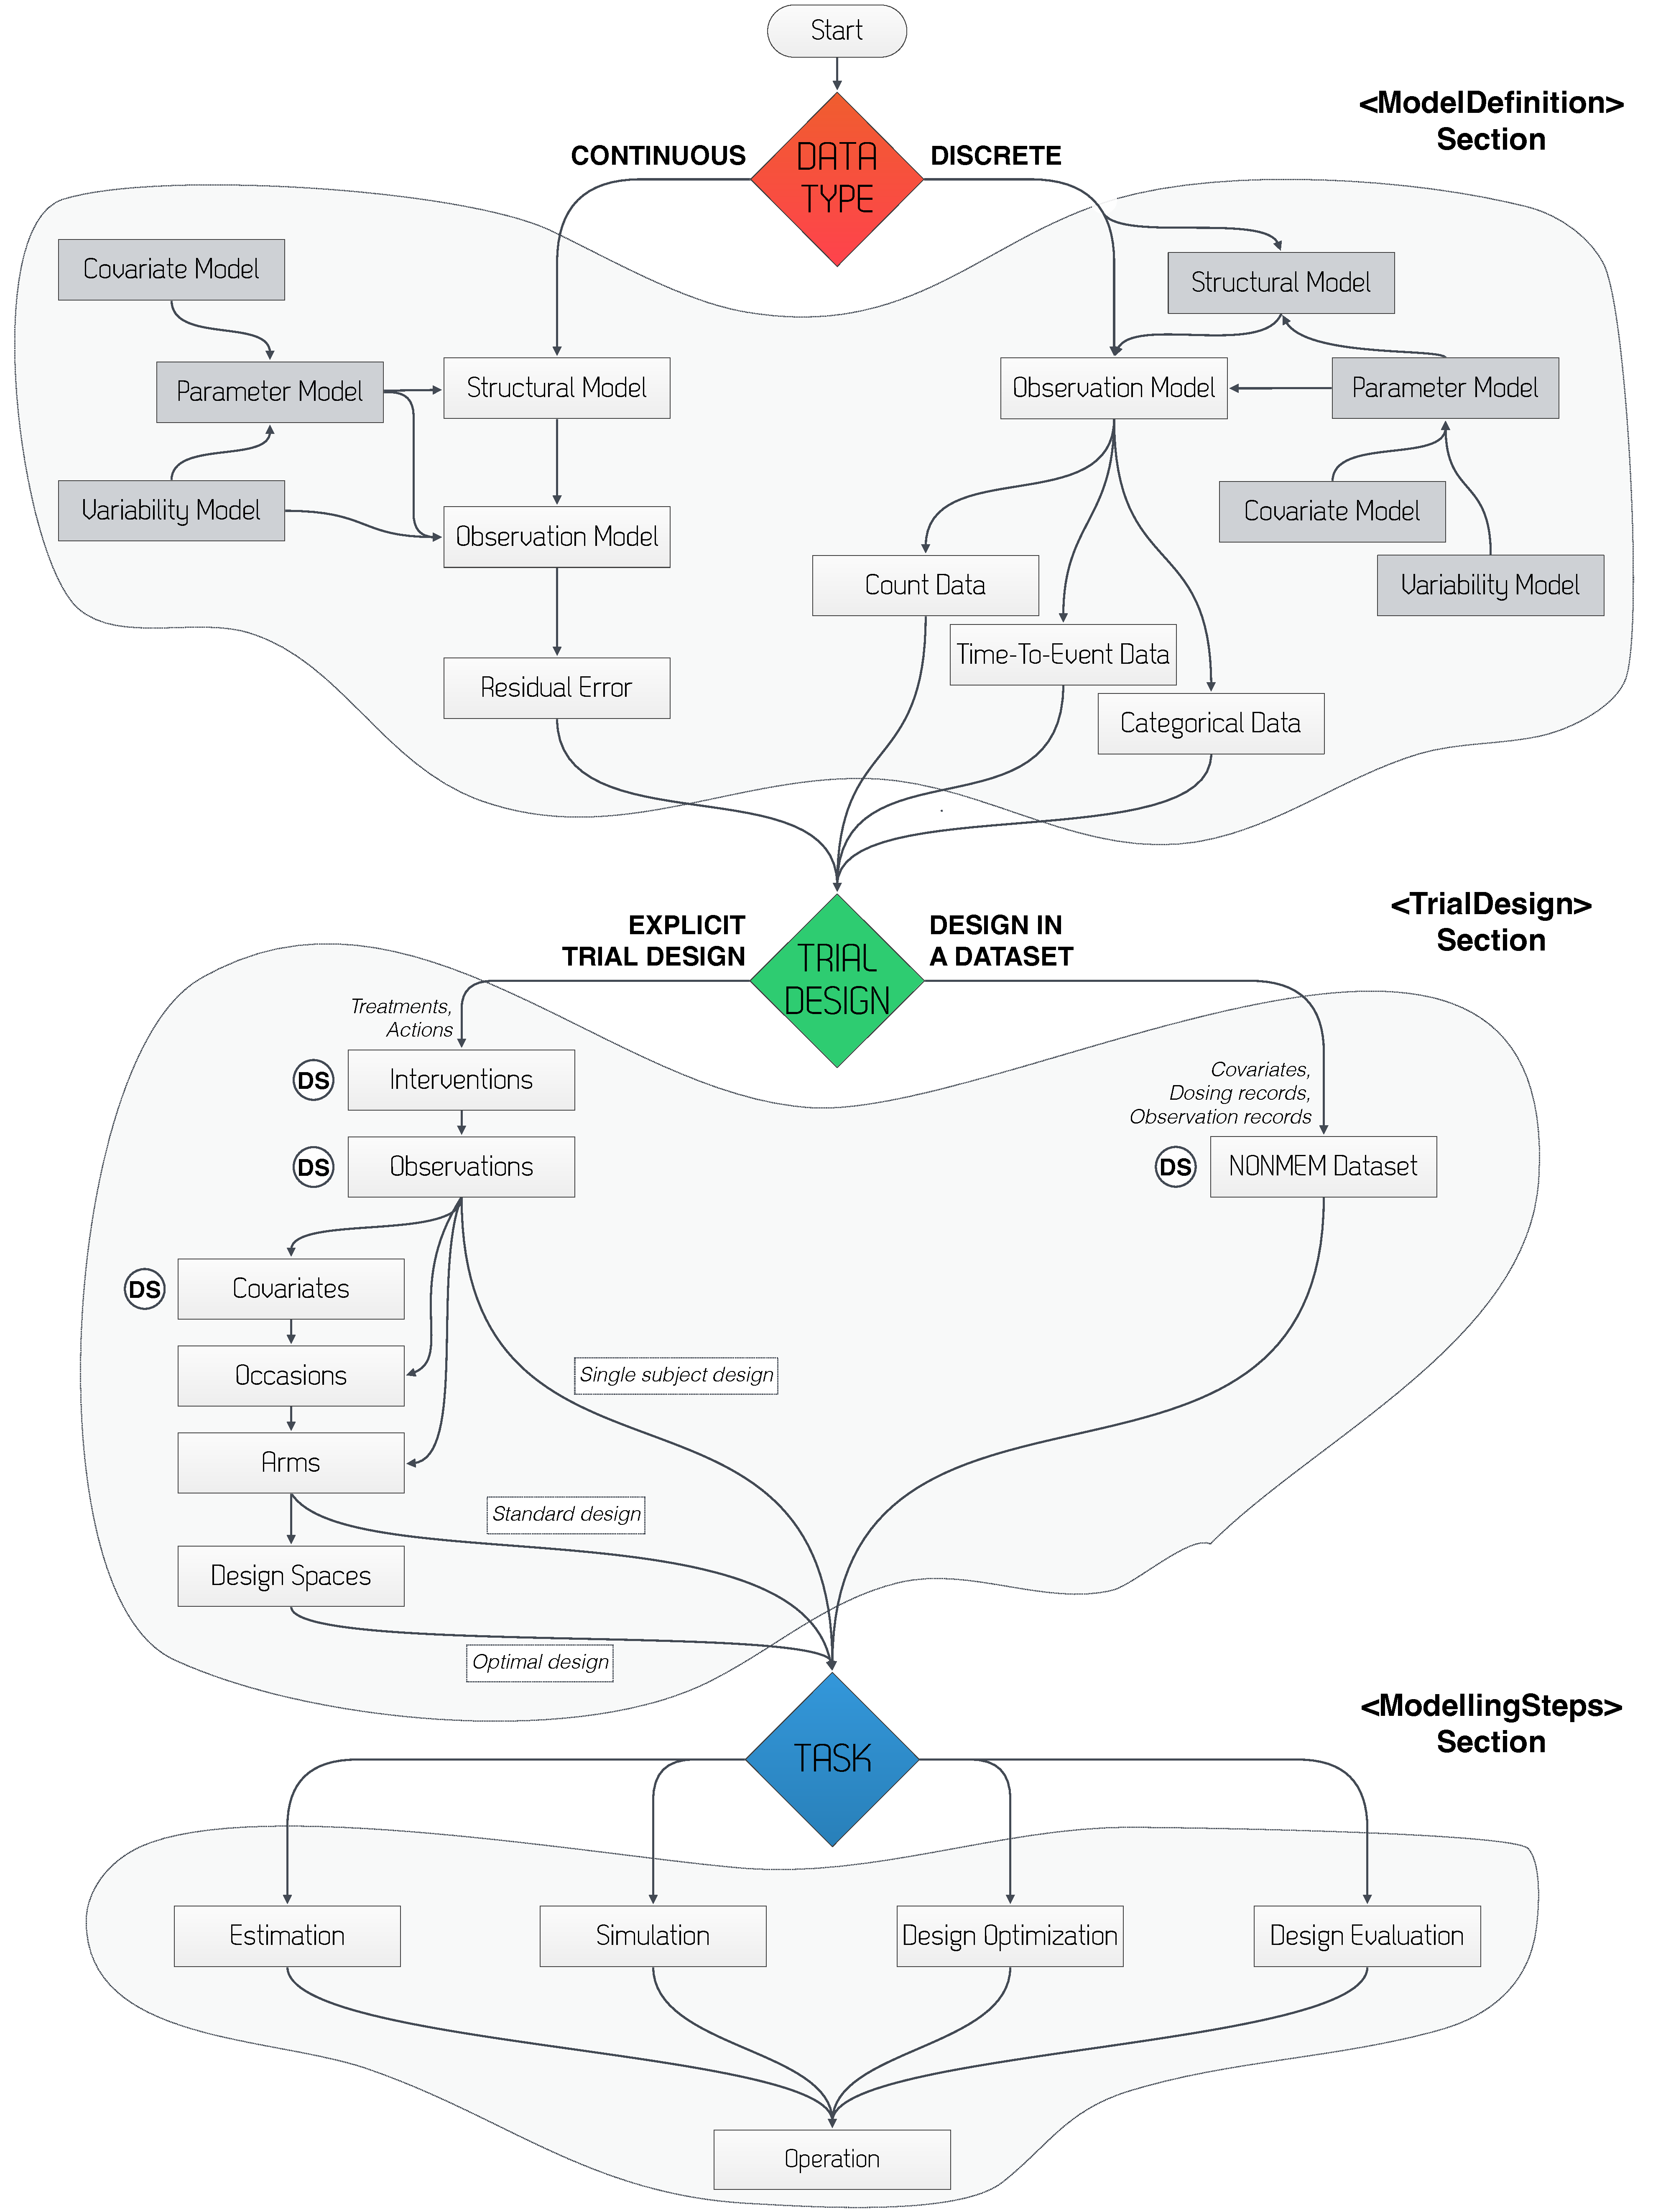
\includegraphics[width=90mm]{pics/Flowchart07}
\end{figure}



\vfill

% Bottom of the page
{\large \today \\}

\end{center}
\end{titlepage} 
%\begin{titlepage}
\begin{center}

% Upper part of the page. The '~' is needed because \\
% only works if a paragraph has started.

\includegraphics[width=0.35\textwidth]{./logo/ddmore_logo}~\\[1cm]

%\textsc{\LARGE }\\[1.5cm]
%
\textsc{\Large Internal Report}\\[0.5cm]

% Title
\HRule \\[0.4cm]
{ \huge \bfseries ProbOnto \\[0.4cm] }

\HRule \\[1.5cm]

% Author and supervisor
\begin{minipage}{0.5\textwidth}
\begin{flushleft} \large
\emph{Authors:}\\
Maciej J \textsc{Swat}, EMBL-EBI\\
Pierre \textsc{Grenon}, UCL\\
%Florent \textsc{Yvon}\\
%Sarala \textsc{Wimalaratne}\\
%Niels Rode \textsc{Kristensen}\\
\end{flushleft}
\end{minipage}


\vfill

% Bottom of the page
{\large \today \\}

\end{center}
\end{titlepage} 

\linenumbers
\tableofcontents


%%%%%%%%%%%%%%%%%%%%%%%%%%%%%%%%%%%%%%%%%%%%%%%%%%%%%%%%%%%%%%%%%%%%%%%
%%%%%%%%%%%%%%%%%%%%%%%%%%%%%%%%%%%%%%%%%%%%%%%%%%%%%%%%%%%%%%%%%%%%%%%%
%%%%%%%%%%%%%%%%%%%%%%%%%%%%%%%%%%%%%%%%%%%%%%%%%%%%%%%%%%%%%%%%%%%%%%%%
%%%%%%%%%%%%%%%%%%%%%%%%%%%%%%%%%%%%%%%%%%%%%%%%%%%%%%%%%%%%%%%%%%%%%%%%
%\chapter{Overview}
%
%This document describes extensions and changes in \pml compared to the
%previously released version 0.6.
%
%
%\section{Major changes/extensions in version 0.7 -- {\color{red} \scshape{under construction}}}
%The following table summarises the changes described in detail in following chapters.
%
%\captionsetup[longtable]{skip=1em}
%\LTcapwidth=\textwidth
%\begin{center}
%%\renewcommand{\arraystretch}{1.1}%
%\begin{longtable}{lll}
%\hline
%\hline
%\pml element 				&  version $\le$ 0.6 				& version 0.7 \\
%or modelling aspect 			& 							& \\
%\hline
%\hline
%  \multicolumn{3}{c}{\textit{ProbOnto}}		\\
%\hline
%\hline
%Probability distributions		& \uncertml used for encoding of 	& {\color{red} \scshape{new}} \xelem{Distribution} element with  \\
%						& distributions					& children \xelem{ProbOnto} and \xelem{UncertML} \\
%\hline
%Annotation and encoding of 	&  	--						& \emph{ProbOnto} - ontology and knowledge base \\
%statistical models			&							& o fprobability distribution 	\\
%						& 							& -- support for expressions as parameters \\
%						& 							& -- support for distribution functions \\
%						&							&  and quantities \\
%						&							& -- more then 50 discrete and continuous \\
%						&							& distributions and/or alternative  \\
%						&							& parameterisations \\
%\hline
%\hline
%  \multicolumn{3}{c}{\textit{Models}}		\\
%\hline
%\hline
%Covariates, parameters and 	& not available					& {\color{red} \scshape{new}} 'Distribution'-type model\\
%observations model  		&							& can be used with either \uncertml or \\
%			 			&							& ProbOnto for parameters, observations and \\
%						&							& covariates \\
%\hline
%Individual parameter model	& 3 types supported: 'Equation'	& 4 types supported now \\
%						& type, Gaussian with linear/ 		& -- \xelem{GaussianModel} renamed to   \\
%						& nonlinear covariate model		& \xelem{StructuredModel} with linear/nonlinear \\
%						&							& covariate model {\color{red} \scshape{modified}}\\
%						&							& -- 'Equation' type (no changes) \\
%						&							& -- {\color{red} \scshape{new}} 'Distribution' type model using  \\
%						&							& either UncertML or ProbOnto \\
%						&							& -- \xelem{PopulationParameter} element \\
%						&							& renamed to \xelem{PopulationValue} \\
%\hline
%Population parameter		& \xelem{SimpleParameter} used	&{\color{red} \scshape{new}}  \xelem{PopulationParameter} element \\	
%						& with no distribution support		& \xelem{SimpleParameter} element removed \\
%						&							& and replaced by \xelem{PopulationParameter}\\			
%\hline
%Covariate model			& Transformation, interpolation  	& {\color{red} \scshape{new}} Support for conditional distributions \\
%						& and distribution of covariates 	& wrt covariates or design elements  \\
%						& supported					& \\
%\hline
%Matrix/Vector operators		& not supported				& Added inverse, trace and transpose \\
%						&							& operators {\color{red} \scshape{new}} \\
%\hline
%Bayesian inference and		& not supported				& \\
%hierarchical models			& 							& \\
%\hline
%\hline
%  \multicolumn{3}{c}{\textit{TRIAL DESIGN}}  \\
%\hline
%\hline
%Lookup table 				& Available in \xelem{Administration}& Moved to \xelem{Observations} \\
%\hline
%Simulation Step			& not available					&  \xelem{InterventionsReference} element {\color{red} \scshape{new}}\\
%\hline
%\hline
%  \multicolumn{3}{c}{\textit{GENERAL}}  \\
%\hline
%\hline
%Interval					& not available					& Element \xelem{Interval} with left/right- \\
%						&							& endpoints of closed/open \xatt{type} attribute. \\
%						&							& \xatt{closed} is the default value. \\
%\hline
%\caption{Overview of major differences between versions 0.7 and 0.6}
%\label{figTable:overviewTable}
%\vspace{-2em}
%\end{longtable}
%\end{center}
%

%\paragraph{Covariate model}
%Covariate model is barely covered so far. See also \cite{Keizer:2011aa}. Missing are following features:\\
%For categorical covariates:\\
%-- categorical distribution of categorical covariates \\
%---- estimating categorical distribution from external data file -- TEST \\
%---- sampling from known categorical distribution -- TEST \\
%---- clusters of categorical covariates \\
%For continuous covariates:\\
%-- power-normal distribution for continuous covariates \\
%---- estimating parameters $\lambda$,$\mu$,$\sigma$ from external data file \\
%---- sampling from known power-normal distribution \\
%---- conditional distribution of continuous covariates - DONE \\
%---- selecting criteria for continuous covariates \\
%---- dependent distribution of continuous covariates \\
%---- correlated continuous covariates \\
%For both types: \\
%-- selection/exclusion criteria missing \\


%%%%%%%%%%%%%%%%%%%%%%%%%%%%%%%%%%%%%%%%%%%%%%%%%%%%%%%%%%%%%%%%%%%%%%
%%%%%%%%%%%%%%%%%%%%%%%%%%%%%%%%%%%%%%%%%%%%%%%%%%%%%%%%%%%%%%%%%%%%%%%
%%%%%%%%%%%%%%%%%%%%%%%%%%%%%%%%%%%%%%%%%%%%%%%%%%%%%%%%%%%%%%%%%%%%%%%
%%%%%%%%%%%%%%%%%%%%%%%%%%%%%%%%%%%%%%%%%%%%%%%%%%%%%%%%%%%%%%%%%%%%%%%
\chapter{\emph{ProbOnto} -- Ontology/Knowledge Base of Probability Distributions}
\label{ch:ProbOnto}


\paragraph{Background}
When encoding probabilistic uncertainties using a parametric distribution its name and 
parameters are sufficient to specify it in an unambiguous way as 
in most cases such parameter set is unique. But, because for a number of cases 
two or more parameterisations exist, one needs to be precise what 
parameters are used when referring to a distribution, otherwise one might 
end up with a wrong model (see for an example Figure \ref{fig:whatCanGoWrong}).
For this purpose an external standard reference is very useful as it allows to 
considerably reduce the effort of declaring the required distribution in a language 
such as MDL or PharmML.

\begin{figure}[htb!]
\centering
\begin{tabular}{cc}
 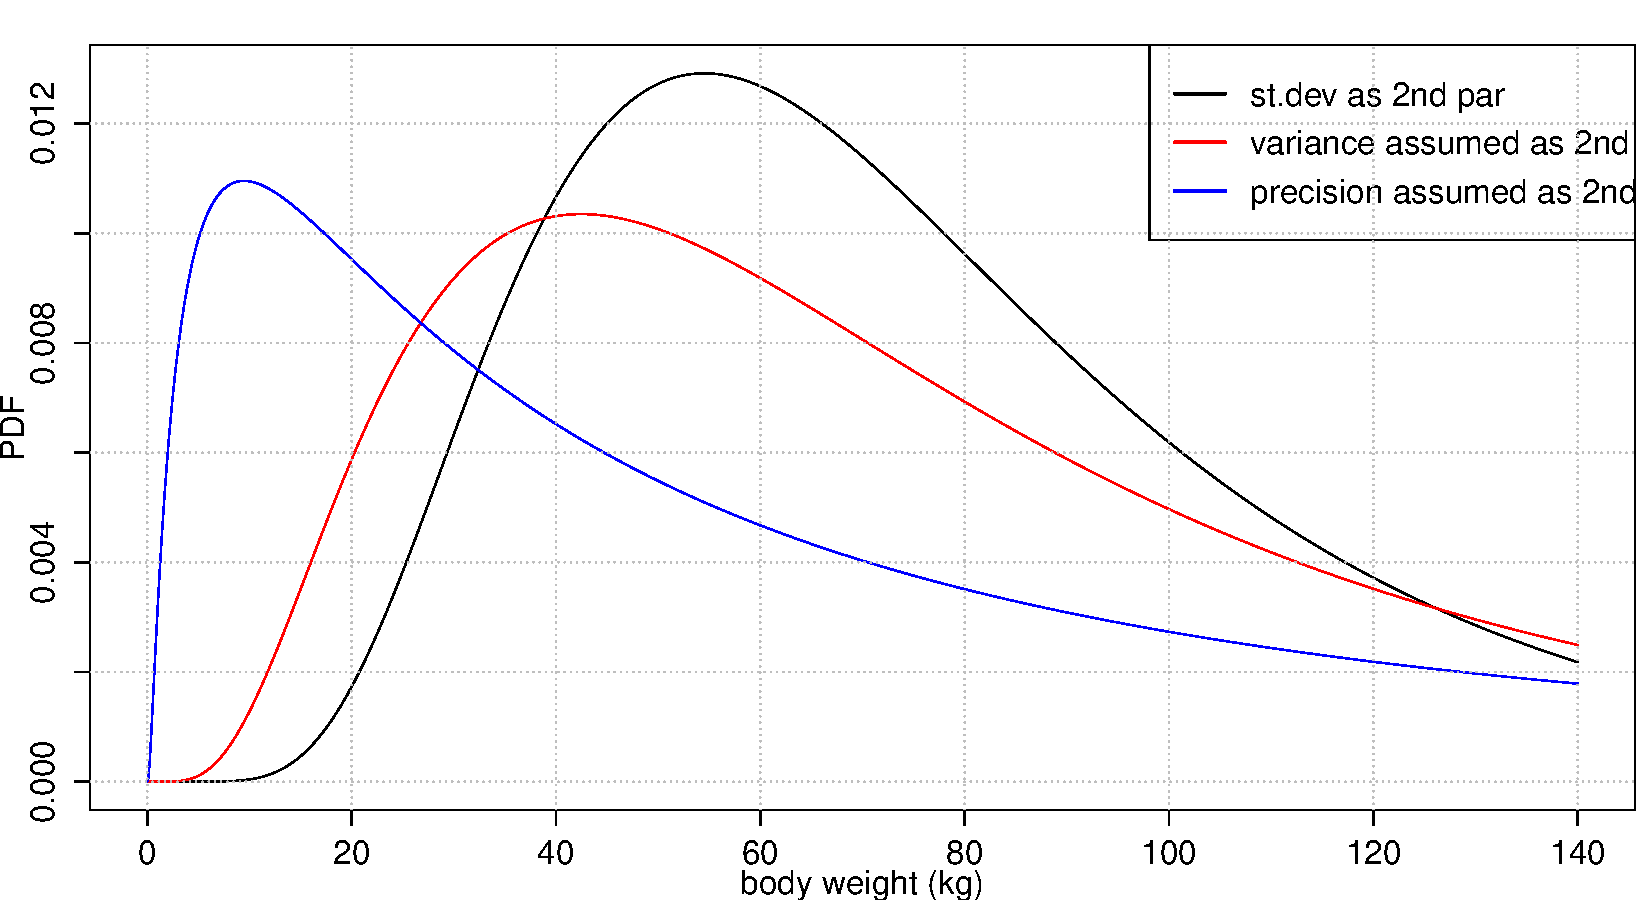
\includegraphics[width=100mm]{pics/whatCanGoWrong}
\end{tabular}
\caption{Illustration of possible model misspecification when using incorrect 
parameterisation. (1) The black curve corresponds to a log-normal 
distribution of body weight, $\mathcal {LN}(\mu\!=\!\log(70),\sigma\!=\!0.5)$, the 
intended parameterisation. (2) Here it was mistakenly assumed that 0.5 corresponds 
to the variance and calculation of standard deviation as required by the R function 
\emph{dlnorm} gives $\sigma = \sqrt{0.5}=0.707$ (red). (3) Here the modeller 
assumed that the 2nd input value corresponds to the precision and calculated the 
standard deviation as $\sigma = 1/\sqrt{0.5}=1.41$ (blue). Small numerical 
differences in $\sigma$, on the log-scale, result in significant differences on the natural scale.}
\label{fig:whatCanGoWrong}
\end{figure}

Until now, we have been relying on the UncertML, \cite{uncertml3:2014}, 
which provides means to encode in MDL/PharmML a range of continuous and 
discrete uni/multi-variate probability distributions. However, from the perspective 
of PharmML, it has several limitations as described in section \ref{sec:uncertmlLimits}. 

\paragraph{Idea} The initial motivation for \emph{ProbOnto} was to create an ontology of probability 
distributions purely for annotation purposes. Many resources are available online 
and in printed format but no proper ontology exists so far\footnote{For 
example, the Statistics Ontology, STATO, \url{http://stato-ontology.org/}, provides 
for most distributions merely a link to an external reference/definition. No parameters
or related functions and quantities are defined in the ontology making their annotation
impossible. Other ontologies, we have analysed number of them featured in the 
BioPortal, \cite{noy2009bioportal}, suffer from equivalent limitations
as they are designed in a similar way.}.  
Similarly, the databases of distributions available online come with similar issues\footnote{Distributome, 
\url{http://www.distributome.org/}, comes with an impressive and well referenced collection
of 90+ distributions but doesn't contain many of relevant for us cases and/or 
parameterisations and is limited to univariate parametric ones.}.
It turns out that \emph{ProbOnto} can be very helpful in
designing a flexible alternative for UncertML with many additional features.
It turns out that it can be used e.g. in PharmML or other target tools/languages \emph{both} 
as ontological resource for annotation purposes and as a knowledge base, 
see next section for their definitions, to provide the means to specify a wide range 
of distributions and distribution related functions and quantities.

In fact, such solution is indispensable in the face of requirements 
posed by models we would like to encode currently and in the foreseeable future. 

%%%%%%%%%%%%%%%%%%%%%%%%%%%%%%%%%%%%%%%%%%%%%%%%%%%%%%%%%%%%%%%%%%%%%%
\section{Ontology versus Knowledge Base}
\begin{description}
\item[Ontology] is a formal representation of a domain of knowledge. It is an abstract entity 
defining the vocabulary for a domain and the relations between concepts.
However, an ontology doesn't specify how that knowledge is stored 
(as physical file, in a database, or in some other form), and how the knowledge 
can be accessed.
\item[Knowledge base] is a physical artifact. It is a database, a repository of information 
that can be accessed and manipulated in some predefined fashion.
\end{description}
The knowledge in a knowledge base is modelled according to rules and relationships 
defined in an ontology.

%%%%%%%%%%%%%%%%%%%%%%%%%%%%%%%%%%%%%%%%%%%%%%%%%%%%%%%%%%%%%%%%%%%%%%
\section{Limitations of the application of UncertML in PharmML}
\label{sec:uncertmlLimits}
Although very useful to a certain extent, there are limitations in
the design and scope of UncertML making the encoding of some 
probability distributions cumbersome or even impossible, see examples below. 
Here some known limitations (in the order of severity):
\begin{itemize}
\item
it doesn't support the assignment of expressions for distribution parameters or 
the specification of block references, which is required if the parameter in question 
is defined elsewhere in the model. 
\item
it doesn't cover many distributions used in Pharmacometrics, e.g. 
\begin{itemize}
\item 
multivariate continues distributions such as Inverse-Wishart
\item
discrete distributions such as Generalized Poisson, Zero-inflated Poisson etc.
\item
or alternative parameterisations for distributions such as Negative Binomial, 
Log-Normal etc.
\end{itemize}
\item
\xelem{degreesOfFreedom} parameter element of the Wishart distribution doesn't support
referencing a variable (required for Bayesian inference) -- a known bug/limitation 
but with no solution for now.
\item
UncertML is a reference resource for distributions and does not provide 
mechanisms to retrieve programmatically related functions and
quantities.  
\end{itemize}
Other minor issues:
\begin{itemize}
%\item
%changes/updates in the unpublished version 3.0 happen without providing 
%documentation change-log.
\item
the implementation of \xelem{MultivariateNormalDistribution} requires the specification 
of the \xatt{dimension} attribute of the covariance matrix -- although this can be estimated
it requires unnecessary calculations when translating models to PharmML. 
\item
every extension requires changes in the already complex XML schema.
\item
doesn't support the precision parameter, $\tau$, used in winBUGS  
rather then standard deviation or variance and precision matrix, $T$, instead 
of covariance matrix $\Sigma$, see tables \ref{figTable:univariates} and \ref{figTable:multivariates}.
\item
version 3.0 which we currently use is not yet released publicly, the UncertML website 
is not updated and 3.0 documentation is not available.
\end{itemize}

\paragraph{UncertML extension} A seemingly easy solution would be to extend UncertML 
but to do so, it would mean to introduce major extensions and changes to its 
current XML schema. Only the support of the most important missing features would 
de facto require to rewrite the entire standard, as UncertML doesn't possess the 
structure to support encoding of even basic expressions. And because it would most 
certainly result in a different, compared to PharmML, mathematical notation we would 
be faced with inconsistent, layered and/or overlapping schemas difficult to handle and 
to process.

\paragraph{Suggested way forward} ProbOnto offers an alternative solution allowing
to avoid all the limitations listed above while providing number of additional features
and means to build in a very flexible probability distribution support in MDL and PharmML 
and other languages/tools within DDMoRe and beyond. 

%%%%%%%%%%%%%%%%%%%%%%%%%%%%%%%%%%%%%%%%%%%%%%%%%%%%%%%%%%%%%%%%%%%%%%
\section{ProbOnto Features}
\begin{itemize}
\item
General 
\begin{itemize}
\item
Covers more then 50 distributions and alternative parameterisations.
\item
Supports encoding of mixture distributions and truncation bounds (open/closed).
\item
Allows for easy encoding of distributions and related functions in target 
tools/languages thanks to its generic format.
\item
Doesn't enforce specific implementation in target tools.
\item
In PharmML only few extensions were required to provide flexible encoding support
for all distributions and their features, see section \ref{sec:workingProbOnto}.
\item
Collection of supported distributions, see appendix \ref{ch:probontoAppendix} for 
some selected distributions and their essential features, is easily extendable 
without non or limited impact on the PharmML structure.
\item
Mathematical functions and quantities are encoded in Latex, plain text 
representation is planned.
\end{itemize}
\item
ProbOnto as Ontology
\begin{itemize}
\item
It can be used to annotate statistical models based on supported probability 
distributions, e.g. their name, parameters, truncation bounds, their defining 
functions and quantities.
\end{itemize}
\item
ProbOnto as Knowledge Base
\begin{itemize}
\item
Provides for each distribution either PDF or PMF and in many cases also 
other distribution related functions such as CDF, hazard and survival functions 
-- the level of coverage depends on the particular distribution. 
%see Appendix \ref{ch:probontoAppendix}.
\item
Provides related quantities such as mean, median, mode, variance etc.
\item
Provides other info about \emph{support/range} and relationships to other distributions.
\end{itemize}
\end{itemize}
The distribution collection and their features are based, among others, on
probability distribution pages of the english Wikipedia\footnote{See the list of 
distributions on Wikipedia at \url{https://en.wikipedia.org/wiki/List_of_probability_distributions}}, 
\cite{Forbes:2010jk}, \cite{Leemis:2008tg}, \cite{song2011eighty}, and 
Wolfram MathWorld \cite{weisstein2007wolfram}.

%%%%%%%%%%%%%%%%%%%%%%%%%%%%%%%%%%%%%%%%%%%%%%%%%%%%%%%%%%%%%%%%%%%%%%
\subsection{Features under construction}
The following features are under construction and not available in the current 
release. They are available to certain extend in UncertML, which should be used
for the time being, if required.
\begin{itemize}
\item
truncation bounds -- supported already for all univariate distributions but an extension 
to multivariate distributions is needed.
%\item
%mixture models - added but more testing required -- see example 'Poisson with mixture distribution', PMIX.
\item
non-parametric distributions.
\end{itemize}

%%%%%%%%%%%%%%%%%%%%%%%%%%%%%%%%%%%%%%%%%%%%%%%%%%%%%%%%%%%%%%%%%%%%%%%
\section{Working with ProbOnto}
\label{sec:workingProbOnto}
The subsequent chapters come with a number of examples of ProbOnto use
but it is worth to point out two basic implementation rules 
\begin{itemize}
\item 
The name of a distribution, encoded in the \xelem{DistributionName} tag, 
must be one of the 'Code names' assigned to each distribution in ProbOnto
using the \xatt{name} attribute. 
\item
The same holds of the parameters of a distribution, encoded in the \xelem{Parameter} tag.
The parameter 'Code names' are specified using also a \xatt{name} attribute. 
The order of parameters doesn't matter. 
\end{itemize}
We have found instances of different names being used for the same parameters 
of many distributions, see for example discussion in section \ref{par:poissonParameterNames}. 
The majority of parameter names is identical to those used in UncertML.
This is to keep the nomenclature consistent within PharmML and MDL, where
the UncertML vocabulary is mostly used.

In tables \ref{figTable:univariates} -- \ref{figTable:multivariatesCodes} and \ref{figTable:mixtures} 
we have compiled the 'Code names'. Multiple examples in this and next sections/chapters 
how to apply the above rules in implement the distributions.

\begin{example}
The negative binomial implementation illustrates how this works. There are two 
parametrisations for this distribution but the one with Poisson intensity, $\lambda$, 
and over-dispersion, $\tau$, as parameters, with the code name, \emph{NegativeBinomial2}, 
is frequently used in discrete data models.
\lstset{language=XML}
\begin{lstlisting}
    <Distribution>
        <ProbOnto name="NegativeBinomial1">
            <!-- Poisson intensity -->
            <Parameter name="rate">
                <ct:Assign>
                    <ct:SymbRef blkIdRef="pm1" symbIdRef="rabbit"/>
                </ct:Assign>
            </Parameter>
            <!-- overdispersion -->
            <Parameter name="overdispersion">
                <ct:Assign>
                    <ct:SymbRef blkIdRef="pm2" symbIdRef="piggy"/>
                </ct:Assign>
            </Parameter>
        </ProbOnto>
    </Distribution>
\end{lstlisting}
%	
According to the rules, the names of the distributions and their parameters 
must be the code names defined by ProbOnto, see table \ref{figTable:multivariatesCodes}. 
The user can then assign any symbols to the parameters,
such as \emph{rabbit} stands for \emph{rate}, defined in 
parameter model \xatt{pm1} and \emph{piggy} for \emph{overdispersion}, 
defined in parameter model \xatt{pm2}.
%effort required in PharmML and other target 
%tools to make use of ProbOnto is reduced to minimum.
\end{example}

\subsection{New elements supporting ProbOnto}
The following elements are new in this version
\begin{itemize}
\item
\xelem{ProbOnto} with the \xatt{name} attribute for the distribution code names, see tables 
\ref{figTable:univariatesCodes} and \ref{figTable:multivariatesCodes} with children elements
\begin{itemize}
\item
\xelem{Parameter}  with the \xatt{name} attribute for the parameter code names, see tables 
\ref{figTable:univariatesCodes} and \ref{figTable:multivariatesCodes}.
\item
\xelem{LowerTruncationBound} and \xelem{LowerTruncationBound} to indicate the
truncation bounds for univariate distributions with attribute \xatt{type} which can
be either \emph{closed} or \emph{open}.
\item
\xelem{MixtureComponent} with the \xatt{name} attribute of the code name of mixture 
components.
\end{itemize}
\end{itemize}


%%%%%%%%%%%%%%%%%%%%%%%%%%%%%%%%%%%%%%%%%%%%%%%%%%%%%%%%%%%%%%%%%%%%%%%
\section{Alternative parameterisations -- examples}
Providing alternative parameterisations is required for number of reasons, such as
model type, application area, available data and target tool -- e.g. BUGS using 
precision, $\tau$, rather then standard deviation or variance for a number of 
distributions. (See also a discussion on parameters difference between BUGS
and R, \cite{lebauer2013translating}). A few typical examples are given in next section.

\subsection{Negative binomial distribution}
See the Wikipedia article\footnote{\url{en.wikipedia.org/wiki/Negative_binomial_distribution}, 
section 'Alternative formulations'}, explaining the reasons behind the various representations. 
The available parameterisations, among others, are
\begin{itemize}
\item
NegativeBinomial1\,($r$, $p$) with r -- \emph{number of failures} and p -- \emph{success probability},
\begin{align}
P(y=k;r,p) = \binom {k+r-1}k (1-p)^r p^k \nonumber
\end{align}
\item
NegativeBinomial2\,($\lambda$, $\tau$) with $\lambda$ -- \emph{Poisson intensity} and $\tau$ -- \emph{over-dispersion},
\begin{align}
P(y=k;\lambda,\tau) = \frac{\Gamma(k + \frac{1}{\tau})}{k!\; \Gamma(\frac{1}{\tau})} \Big(\frac{1}{1+\tau \lambda} \Big)^{\frac{1}{\tau}} 
\Big(\frac{\lambda}{\frac{1}{\tau} + \lambda} \Big)^{k} \nonumber
\end{align}
%\item
%NegativeBinomial3\,($\lambda$, $\theta$) with $\lambda$ -- \emph{Poisson intensity} and $\theta$,
%\begin{align}
%\frac{\Gamma(\theta + y)}{\Gamma(a)\Gamma(y+1)} \Big(\frac{\theta}{\theta + \mu} \Big)^{\theta} 
%\Big(\frac{\mu}{\theta + \mu} \Big)^{y} \nonumber
%\end{align}
\end{itemize}
with the latter being used in typical pharmacometric discrete data models, \cite{Plan:2009fk, Troconiz:2009fv}.
\subsection{Normal distribution}
Available parameterisations, see Table \ref{figTable:logNormalParameterisations}, are
\begin{itemize}
\item
Normal1\,($\mu$, $\sigma$) with $\mu$ -- \emph{mean} and $\sigma$ -- \emph{standard deviation}, 
\item
Normal2\,($\mu$, \emph{v}) with $\mu$ -- \emph{mean} and \emph{v} -- \emph{variance},
\item
Normal3\,($\mu$, $\tau$) with $\mu$ -- \emph{mean} and $\tau$ -- \emph{precision} ($\tau=1/\sigma^2$)
\end{itemize}

\subsubsection{Re-parameterisation formulas}
In this case the recalculation between the representation is very simple
but is given here for the completeness.
\begin{itemize}
\item 
\begin{description}
\item[N1($\mu$, $\sigma$) $\rightarrow$ N2($\mu$, $v$)]:
$\mu \rightarrow \mu; \quad \sigma \rightarrow v=\sigma^2$

\item[N2($\mu$, $v$) $\rightarrow$ N1($\mu$, $\sigma$)]:
$\mu \rightarrow \mu; \quad v \rightarrow \sigma = \sqrt{v}$
\end{description}

\item 
\begin{description}
\item[N1($\mu$, $\sigma$) $\rightarrow$ N3($\mu$, $\tau$)]:
$\mu \rightarrow \mu; \quad \sigma \rightarrow \tau=1/\sigma^2$

\item[N3($\mu$, $\tau$) $\rightarrow$ N1($\mu$, $\sigma$)]:
$\mu \rightarrow \mu; \quad \tau \rightarrow \sigma=1/\sqrt{\tau}$
\end{description}

\item 
\begin{description}
\item[N2($\mu$, $v$) $\rightarrow$ N3($\mu$, $\tau$)]:
$\mu \rightarrow \mu; \quad v \rightarrow \tau=1/v$

\item[N3($\mu$, $\tau$) $\rightarrow$ N2($\mu$, $v$)]:
$\mu \rightarrow \mu; \quad \tau \rightarrow v=1/\tau$
\end{description}
\end{itemize}

\begin{figure}[htb!]
\centering
\begin{tabular}{cc}
% \includegraphics[width=140mm]{pics/CDF_17Dec} \\
 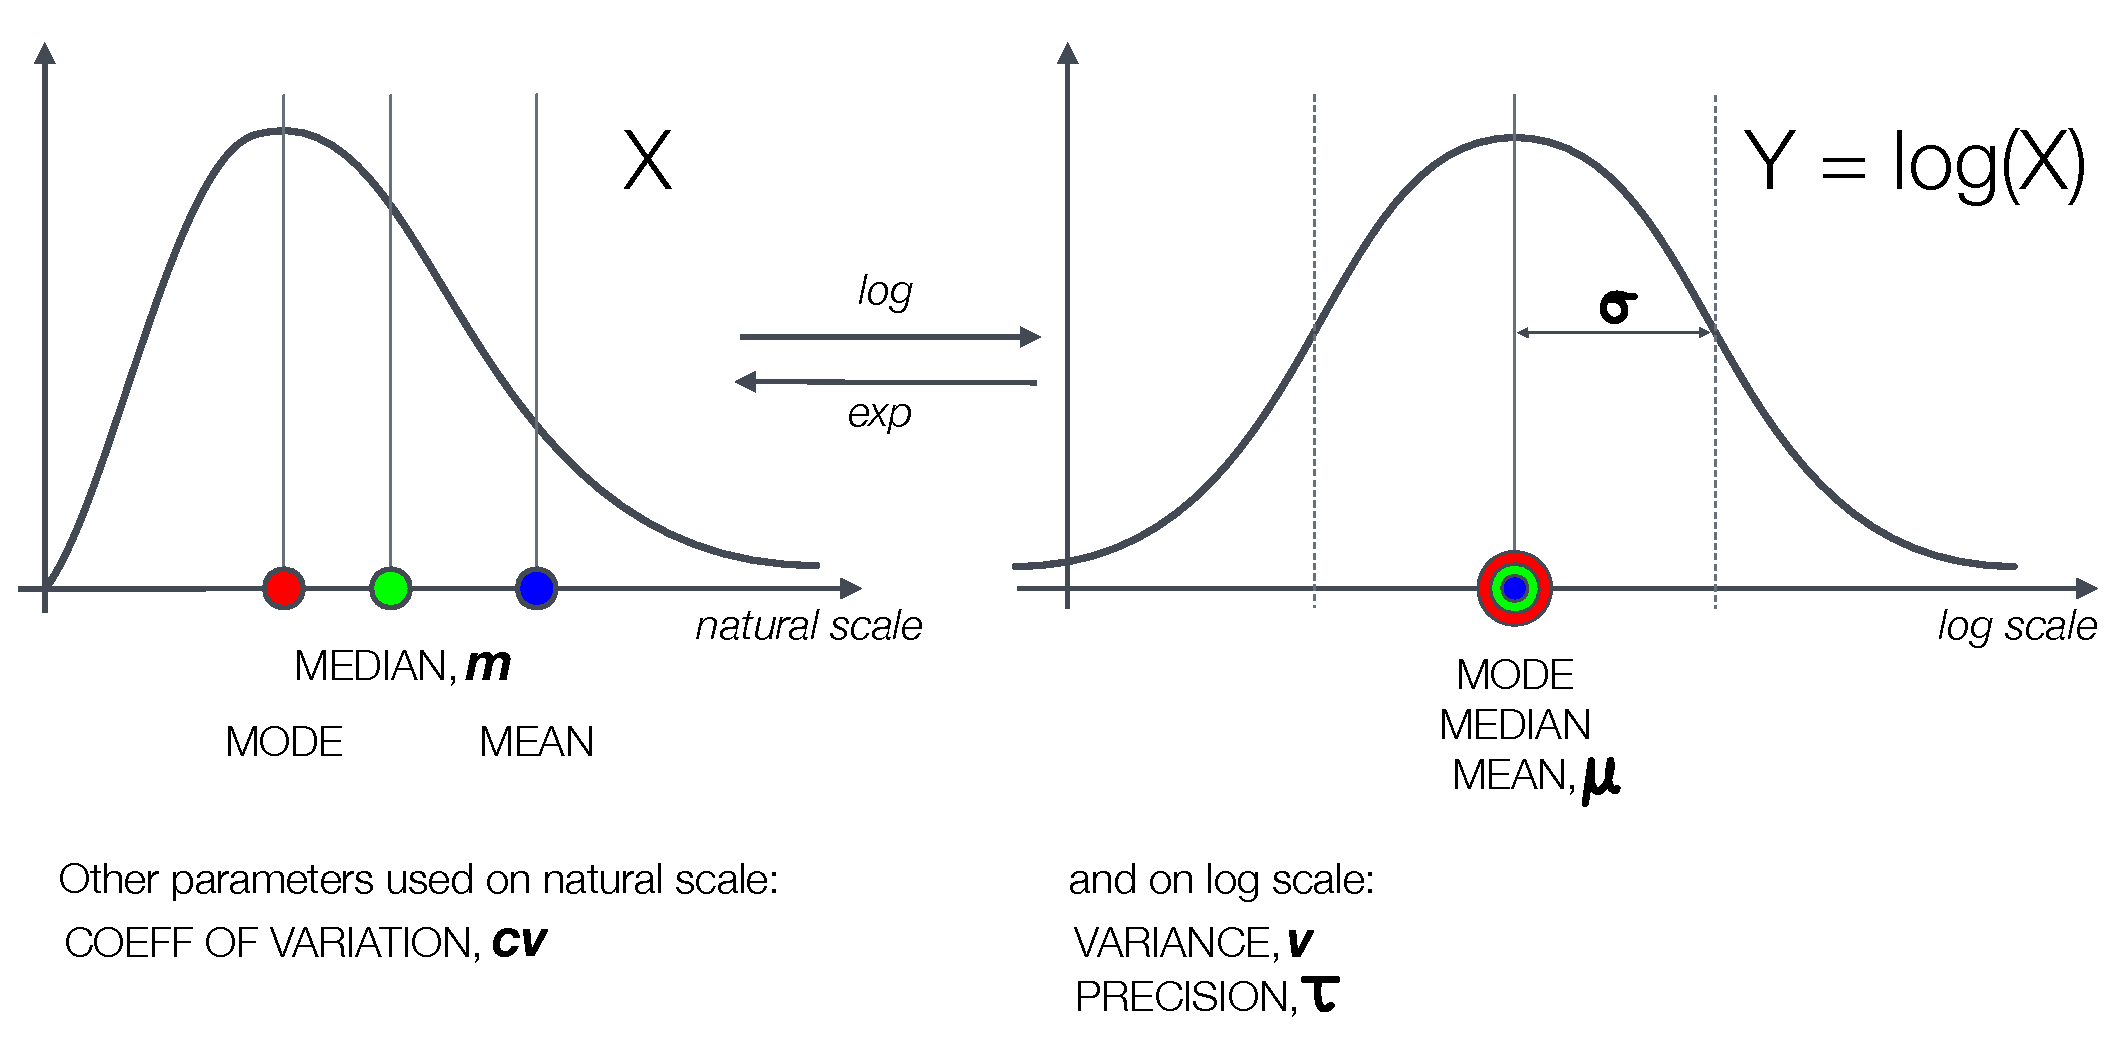
\includegraphics[width=160mm]{pics/normalAndLogDomain_schema}
\end{tabular}
\caption{Schematic representation of the lognormaly distributed data on the natural (left) 
and logarithmic scale (right), see Figure \ref{fig:insulinData} for real-life data example. 
\textbf{Bold} symbols stand for quantities commonly used to parameterise a log-normally 
distributed variable.}
\label{fig:schematicLogNormal}
\end{figure}

\subsection{Log-normal distribution}
\label{subsec:logNormalForms}
The log-normal distribution is special in that not only different parameter sets exist
but also because they are defined either on the natural or logarithmic scale. Interestingly, in one 
case the parameters are defined on two different scales, see Figure \ref{fig:schematicLogNormal},
for an overview.\\
Available parameterisations (also listed in Table \ref{figTable:univariates} 
with indication about their coverage in target tools) are 
\begin{itemize}
\item
LogNormal1\,($\mu$, $\sigma$) with \emph{mean}, $\mu$, and \emph{standard deviation}, $\sigma$, both on the log-scale, 
\item
LogNormal2\,($\mu$, \textit{v}) with \emph{mean}, $\mu$, and \emph{variance}, $v$, both on the log-scale, 
\item
LogNormal3\,(\textit{m}, $\sigma$)  with \emph{median}, $m$, on the natural scale and \emph{standard deviation}, $\sigma$, on the log-scale, 
\item
LogNormal4\,(\textit{m}, \textit{cv}) with \emph{median}, $m$, and \emph{coefficient of variation}, $cv$, both on the natural scale, 
\item
LogNormal5\,($\mu$, $\tau$) with \emph{mean}, $\mu$, and \emph{precision}, $\tau$, both on the log-scale.
\end{itemize}

\begin{figure}[htb!]
\centering
\begin{tabular}{cc}
 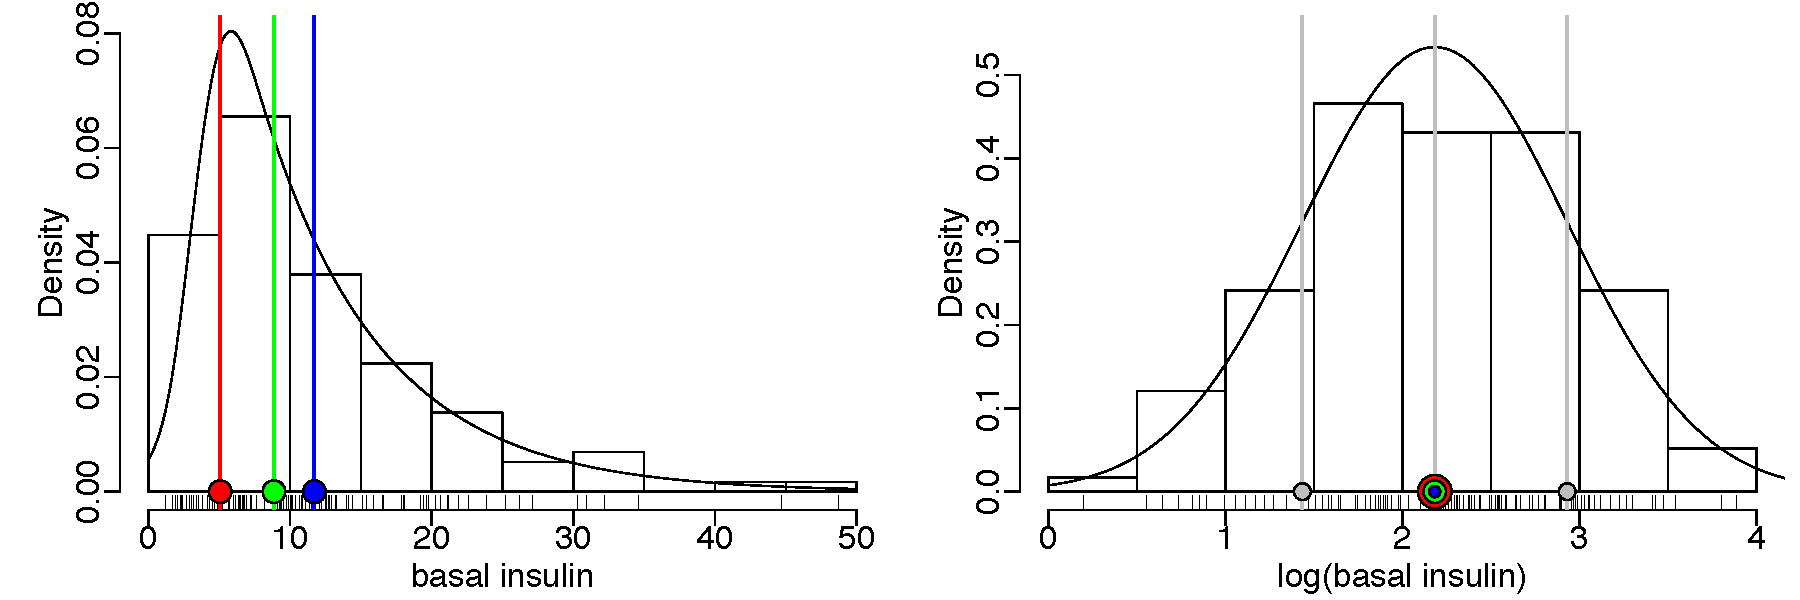
\includegraphics[width=160mm]{pics/normalAndLogDomain}
\end{tabular}
\caption{Representation of the lognormaly distributed basal insulin data in diabetic patients 
\cite{Rudenski:1991aa} on the natural scale (left) and on the logarithmic scale after 
$log$--transformation (right), colour code as in Figure \ref{fig:schematicLogNormal}. 
The density estimation for the data on the natural scale and its plotting was performed 
using the R package \textit{logspline} \cite{Kooperberg:2013}.}
\label{fig:insulinData}
\end{figure}

\subsubsection{Re-parameterisation formulas}
\label{subsubsec:formulas}
The recalculation between given parameterisations is error prone 
and should, if required, be taken over by the converters. The 
following equations might be useful when providing such translation support 
between target tools. For example when translating a model implemented 
for Monolix/NONMEM, which use either LN1 or LN2, with winBUGS as the 
target tool, which uses only LN5.\\
\begin{itemize}
\item 
\begin{description}
\item[LN1($\mu$, $\sigma$) $\rightarrow$ LN2($\mu$, $v$)]:
$\mu \rightarrow \mu; \quad \sigma \rightarrow v=\sigma^2$

\item[LN2($\mu$, $v$) $\rightarrow$ LN1($\mu$, $\sigma$)]:
$\mu \rightarrow \mu; \quad v \rightarrow \sigma = \sqrt{v}$
\end{description}

\item 
\begin{description}
\item[LN1($\mu$, $\sigma$) $\rightarrow$ LN3($m$, $\sigma$)]:
$\mu \rightarrow m=\exp(\mu); \quad \sigma \rightarrow \sigma$

\item[LN3($m$, $\sigma$) $\rightarrow$ LN1($\mu$, $\sigma$)]:
$m \rightarrow \mu=\log(m); \quad \sigma \rightarrow \sigma$
\end{description}

\item 
\begin{description}
\item[LN1($\mu$, $\sigma$) $\rightarrow$ LN4($m$, $cv$)]:
$\mu \rightarrow m=\exp(\mu); \quad \sigma \rightarrow cv=\sqrt{\exp(\sigma^2)-1}$

\item[LN4($m$, $cv$) $\rightarrow$ LN1($\mu$, $\sigma$)]:
$m \rightarrow \mu=\log(m); \quad cv \rightarrow \sigma=\sqrt{\log(cv^2 + 1)}$
\end{description}

\item 
\begin{description}
\item[LN1($\mu$, $\sigma$) $\rightarrow$ LN5($\mu$, $\tau$)]:
$\mu \rightarrow \mu; \quad \sigma \rightarrow \tau=1/\sigma^2$

\item[LN5($\mu$, $\tau$) $\rightarrow$ LN1($\mu$, $\sigma$)]:
$\mu \rightarrow \mu; \quad \tau \rightarrow \sigma=1/\sqrt{\tau}$
\end{description}

\item 
\begin{description}
\item[LN2($\mu$, $v$) $\rightarrow$ LN3($m$, $\sigma$)]:
$\mu \rightarrow m=\exp(\mu); \quad v \rightarrow \sigma=\sqrt{v}$

\item[LN3($m$, $\sigma$) $\rightarrow$ LN2($\mu$, $v$)]:
$m \rightarrow \mu=\log(m); \quad \sigma \rightarrow v=\sigma^2$
\end{description}


\item 
\begin{description}
\item[LN2($\mu$, $v$) $\rightarrow$ LN4($m$, $cv$)]:
$\mu \rightarrow m=\exp(\mu); \quad v \rightarrow cv=\sqrt{\exp(v) -1}$

\item[LN4($m$, $cv$) $\rightarrow$ LN2($\mu$, $v$)]:
$m \rightarrow \mu=\log(m); \quad cv \rightarrow v=\log(cv^2+1)$
\end{description}

\item 
\begin{description}
\item[LN2($\mu$, $v$) $\rightarrow$ LN5($\mu$, $\tau$)]:
$\mu \rightarrow \mu; \quad v \rightarrow \tau=1/v$

\item[LN5($\mu$, $\tau$) $\rightarrow$ LN2($\mu$, $v$)]:
$\mu \rightarrow \mu; \quad \tau \rightarrow v=1/\tau$
\end{description}

\item 
\begin{description}
\item[LN3($m$, $\sigma$) $\rightarrow$ LN4($m$, $cv$)]:
$m \rightarrow m; \quad \sigma \rightarrow cv=\sqrt{\exp(\sigma^2)-1}$

\item[LN4($m$, $cv$) $\rightarrow$ LN3($m$, $\sigma$)]:
$m \rightarrow m; \quad cv \rightarrow \sigma=\sqrt{\log(cv^2 + 1)}$
\end{description}

\item 
\begin{description}
\item[LN3($m$, $\sigma$) $\rightarrow$ LN5($\mu$, $\tau$)]:
$m \rightarrow \mu=\log(m); \quad \sigma \rightarrow \tau=1/\sigma^2$

\item[LN5($\mu$, $\tau$) $\rightarrow$ LN3($m$, $\sigma$)]:
$\mu \rightarrow m=\exp(\mu); \quad \tau \rightarrow \sigma=1/\sqrt{\tau}$
\end{description}

\item 
\begin{description}
\item[LN4($m$, $cv$) $\rightarrow$ LN5($\mu$, $\tau$)]:
$m \rightarrow \mu=\log(m); \quad cv \rightarrow \tau=1/\log(cv^2+1)$

\item[LN5($\mu$, $\tau$) $\rightarrow$ LN4($m$, $cv$)]:
$\mu \rightarrow m; \quad \tau \rightarrow cv=\sqrt{\exp(1/\tau)-1}$
\end{description}
\end{itemize}

The proof of the majority of the formulas is straightforward taking into account the definition
of the parameters in question. The relationship between $\sigma$ or $\tau$ (on the log scale) 
and $cv$ (on the natural scale), essential for the re-calculation formulas involving
LN4 parameterisation, is a bit more tricky to see. The 
proof starts with the known relationships for the mean, $mean$, and variance, $var$, on the natural 
scale, collected with others in table \ref{figTable:logNormalParameterisations}. 
Then the square of the coefficient of variation, $cv$, on the natural scale reads
\begin{align}
	cv^2 &= \frac{var}{mean^2} = \frac{(e^{\sigma^2}-1)\; e^{2\mu + \sigma^2}}{e^{(\mu + 1/2\sigma^2)^2}}
	= (e^{\sigma^2}-1) \Leftrightarrow cv = \sqrt{e^{\sigma^2}-1} \;\;\; \& \;\;\; \sigma=\sqrt{\log(cv^2 + 1)}. \nonumber
%	\frac{\cancel{a= b+c}}{\cancel{f} & = b-c
\end{align}

%\footnote{Based on a Stack Overflow discussion \url{tinyurl.com/qavgvln}}

%\begin{align}
%	\frac{\cancel{a= b+c}}{\cancel{f} & = b-c
%\end{align}



\cleardoublepage
\setlength{\tabcolsep}{2em}
\captionsetup[longtable]{skip=1em}
\LTcapwidth=.95\textwidth
\begin{center}
%\small
\renewcommand{\arraystretch}{1}%
\begin{longtable}{ccc}
 \hline
 \hline
\multicolumn{1}{c}{Log-normal distribution} 	& \multirow{2}{*}{Quantity} 	&\multicolumn{1}{c}{Normal distribution on the} \\ [-.5ex]
\multicolumn{1}{c}{on the natural scale (NS)} 	&						& \multicolumn{1}{c}{log-transformed scale (LS)} \\
   \hline
  \hline
  \multicolumn{3}{c}{$LN1: P(x;\boldsymbol\mu,\boldsymbol\sigma)=\Gape[.5cm][.3cm]{} \frac{1}{x \sigma \sqrt{2 \pi}} \exp\Big[ \frac{-(\log x - \mu)^2}{2\sigma^2}\Big] $ }\\
   \hline
$e^{\mu + \frac{1}{2}\sigma^2}$			& \Gape[.4cm][0cm]{}Mean  	& $\boldsymbol\mu$ \\ [.25ex]
$e^{2\mu + \sigma^2}[e^{\sigma^2}-1]$		& Variance 				& $\sigma^2$	\\ [.25ex]
$e^{\mu + \frac{1}{2}\sigma^2}\sqrt{e^{\sigma^2}-1}$ & Standard deviation	& $\boldsymbol\sigma$	\\ [.25ex]
%									& deviation  				&		 	\\ [.25ex]
 $e^{\mu - \sigma^2}$	 				& Mode 					&	 $\mu$	\\ [.25ex]
$e^\mu$								& Median					& $\mu$ \\ [.25ex]
$\sqrt{e^{\sigma^2}-1}$					& Coefficient of variation		& $\sigma/\mu$ \\ [.5EX]
%									& of variation				& \\
  \hline
  \multicolumn{3}{c}{$LN2: P(x;\boldsymbol\mu,\boldsymbol {v})=\Gape[.5cm][.3cm]{} \frac{1}{x \sqrt{v} \sqrt{2 \pi}} \exp\Big[ \frac{-(\log x - \mu)^2}{2 v}\Big] $ }\\
   \hline
$e^{\mu + \frac{1}{2}v}$					& \Gape[.4cm][0cm]{}Mean  	& $\boldsymbol\mu$ \\ [.25ex]
$e^{2\mu + v}[e^{v}-1]$					& Variance 				& $\boldsymbol v$	\\ [.25ex]
$e^{\mu + \frac{1}{2} v}\sqrt{e^{v}-1}$ 		& Standard deviation		& $ {\sqrt{v}}$	\\ [.25ex]
%									& deviation  				& 	\\ [.25ex]
$e^{\mu - v}$	 						& Mode 					& $\mu$	\\ [.25ex]
$e^\mu$								& Median					& $\mu$ \\ [.25ex]
$\sqrt{e^{v}-1}$						& Coefficient of variation		& ${\sqrt{v}} /\mu$ \\ [.5EX]
%									& of variation				& \\
  \hline
  \multicolumn{3}{c}{$LN3: P(x;\boldsymbol m,\boldsymbol \sigma) =\Gape[.5cm][.3cm]{} \frac{1}{x \sigma \sqrt{2 \pi}} \exp\Big[ \frac{-[\log(x/m)]^2}{2\sigma^2}\Big] $ }\\ %[1.5EX]
   \hline
 $m\, e^{\frac{1}{2}\sigma^2}$				& \Gape[.4cm][0cm]{}Mean  	& $\log( m)$ \\ [.25ex]
 $m^2 e^{\sigma^2} [e^{\sigma^2}-1]$		& Variance 				& $\sigma^2$	\\ [.25ex]
$m\sqrt{e^{\sigma^2} (e^{\sigma^2}-1)}$		& Standard deviation	  	& $\boldsymbol\sigma$	\\ [.25ex]
%									& deviation  				& 	\\ [.25ex]
 $m/e^{\sigma^2}$	 					& Mode 					& $\log( m)$	\\ [.25ex]
 $\boldsymbol m$						& Median 					& $\log( m)$	\\ [.25ex]
$\sqrt{e^{\sigma^2}-1}$					& Coefficient of variation		& $\sigma/\log( m)$ \\ [.5EX]
% 									&  of variation				&  \\
  \hline
   \multicolumn{3}{c}{$LN4: P(x;\boldsymbol m,\boldsymbol {cv})=\Gape[.5cm][.3cm]{} \frac{1}{x \sqrt{\log(cv^2+1)} \sqrt{2 \pi}} \exp\Big[ \frac{-[\log(x/m)]^2}{2\log(cv^2+1)}\Big] $} 	\\
   \hline
 $m \sqrt{cv^2 + 1}$						& \Gape[.4cm][0cm]{}Mean  	& $\log( m)$ \\ [.25ex]
 $m^2 \,(cv^2+1)\,cv^2$					& Variance 				& $\log(cv^2 + 1)$	\\ [.25ex]
$m\,cv \sqrt{(cv^2+1)}$					& Standard  deviation		& $\sqrt{\log(cv^2 + 1)}$	\\ [.25ex]
% 									& deviation  				& 	\\ [.25ex]
 $m / (cv^2 + 1)$	 					& Mode 					& $\log( m)$	\\ [.25ex]
 $\boldsymbol m$						& Median 					& $\log( m)$	\\ [.25ex]
 ${\boldsymbol {cv}}$					& Coefficient of variation		& $\sqrt{\log(cv^2 + 1)}/\log( m)$ \\ [.5EX]
% 									& of variation				&  \\
  \hline
  \multicolumn{3}{c}{$LN5: P(x;\boldsymbol\mu,\boldsymbol \tau)=\Gape[.5cm][.3cm]{} \sqrt{\frac{\tau}{2 \pi}} \frac{1}{x} \exp\Big[ {-\frac{\tau}{2}(\log x-\mu)^2} \Big] $ }\\
   \hline
 $e^{\mu + \frac{1}{2\tau}}$				& \Gape[.4cm][0cm]{}Mean  	& $\boldsymbol\mu$ \\ [.25ex]
 $e^{2\mu + \frac{1}{\tau}}[e^{\frac{1}{\tau}}-1]$ & Variance 			& $1/\tau$	\\ [.25ex]
$e^{\mu + \frac{1}{2} \frac{1}{\tau}}\sqrt{e^{\frac{1}{\tau}}-1}$ 	& Standard deviation & $\sqrt{1/\tau}$	\\ [.25ex]
%									& deviation  				& 	\\ [.25ex]
 $e^{\mu - \frac{1}{\tau}}$					& Mode 					& $\mu$	\\ [.25ex]
 $e^\mu$								& Median					& $\mu$ \\ [.25ex]
%									&						& \\[.25ex]
$\sqrt{e^{\frac{1}{\tau}}-1}$				& Coefficient of variation		& $\sqrt{1/\tau} / \mu$ \\ [.25EX]
%									& of variation				& \\
  $1/\big(e^{2\mu + \frac{1}{\tau}}[e^{\frac{1}{\tau}}-1]\big)$ & Precision				& $\boldsymbol\tau$ \\ [.5ex]
   \hline
\caption{The available parameterisations for the log-normal distribution and their characterising 
quantities as functions of the respective parameters. With $\boldsymbol m$ -- scale parameter (NS), 
$\boldsymbol {cv}$ -- dispersion parameter (NS), $\boldsymbol \mu$ -- mean, location parameter (LS), 
$\boldsymbol \sigma$ -- standard deviation, scale parameter (LS), $\boldsymbol v$ -- variance, scale parameter (LS), 
$\boldsymbol \tau$ -- precision (LS). See Figure \ref{fig:schematicLogNormal} and 
section \ref{subsec:logNormalForms} for the meaning of the symbols.\\ \scriptsize Small print: 
The re-parameterisation formulas, page \pageref{subsubsec:formulas}, and expressions in this table are partially from 
literature, partially calculated (by MJS), use them on your own risk.}
\label{figTable:logNormalParameterisations}
\vspace{-3.5em}
\end{longtable}
\end{center}

\setlength{\tabcolsep}{1em}

\newpage 

\captionsetup[longtable]{skip=1em}
\LTcapwidth=.95\textwidth
\begin{center}
\setlength{\tabcolsep}{7pt}
%\small
\renewcommand{\arraystretch}{1.1}%
\begin{longtable}{l | lcccc}
  \hline
  \hline
\multicolumn{1}{c}{\textbf{ProbOnto}}& Parameters 	& \textbf{UncertML} 	& \textbf{WinBUGS}	& \textbf{Monolix} & \textbf{NONMEM} \\
\multicolumn{1}{c}{0.2}			&		&  3.0			& 1.4		& 4.3	& 7.3 \\
  \hline
  \hline
  \multicolumn{6}{c}{\textit{Discrete Univariate}}  \\
  \hline
Bernoulli				& \emph{p}		&	y	&	y	& --  &  -- \\
Binomial				& \emph{n, p}		&	y	&	y	& --  &  -- \\
Categorical ordered		& $p_1, \ldots, p_k$	& y	&	y	& --  &  -- \\
Categorical unordered	& $p_1, \ldots, p_k$	&	y	&	y	& --  &  -- \\
Generalized Poisson	& $\lambda, \delta$	& --  & --  & --  &  -- \\
Geometric			& \emph{p}		&	y	& --  & --  &  -- \\
Hypergeometric		& \emph{N, K, n}	&	y	& --  & --  &  -- \\
Negative Binomial 1		& \emph{r, p}		&	y	&	y	& --  &  -- \\
Negative Binomial 2 		& $\lambda, \tau$ 	& --  & --  & --  &  -- \\
%Negative Binomial 3 		& $\lambda, \theta$ 	& --  & --  & --  &  -- \\
Poisson				& $\lambda$		&	y	&	y	& --  &  -- \\
Uniform 1 (discrete)		&  \emph{a, b}		& --	& --	& -- & --  \\
Uniform 2 (discrete)		&  0, \emph{n}		& --	& --	& -- & --  \\
Zero-inflated Poisson	& $\lambda, \pi$	& --  & --  & --  &  -- \\
%Zero-Inflated Negative Binomial & $\mu, \theta, p$	& --  & --  & --  &  -- \\
  \hline
  \multicolumn{6}{c}{\textit{Continuous Univariate}}	\\
  \hline
Beta					& $\alpha, \beta$	&	y	&	y	&	y	&  -- \\
Cauchy				& $x_0, \gamma$	&	y	& --  & --  &  -- \\
Chi-squared			& \emph{k}		&	y	&	y	&	y	&  -- \\
%Dirac Delta			&	&	y	& --  & --  &  -- \\
Exponential			& $\lambda$		&	y	&	y	&	y	&  -- \\
F (aka Fisher-Snedecor)	& $d_1, d_2$		&	y	& --  &	y	&  -- \\
Gamma				& $k, \theta$		&	y	&	y	&	y	&  -- \\
Generalized Gamma	& \emph{a, d, p}	&	y	& --  & --  & --	  \\
Gompertz				& $\eta, b$		& --  &	y	& --  & --	  \\
Gumbel (aka Extreme Value)	& $\mu, \beta$	& --  &	y 	& --  & -- \\ 
Inverse-Gamma		& $\alpha, \beta$	&	y	& --  & --  &  -- \\
Laplace 1				& \multirow{2}{*}{$\mu, b$} &	\multirow{2}{*}{y}	&	\multirow{2}{*}{--}	& \multirow{2}{*}{--}  & \multirow{2}{*}{--} \\ [-0.5ex]
(Double-exponential 1) \\
Laplace 2				& \multirow{2}{*}{$\mu, \tau$} &	\multirow{2}{*}{--}	&	\multirow{2}{*}{y}	& \multirow{2}{*}{--}  & \multirow{2}{*}{--} \\ [-0.5ex]
(Double-exponential 2) \\[0.5ex]
Log-Normal 1			& $\mu, \sigma$	&	y	&	--	&	y	&  -- \\
Log-Normal 2			& $\mu$, \textit{v}	&	y	&	--	&	y	&  -- \\
Log-Normal 3			& \emph{m}, $\sigma$	&	--	&	--	&	--	&  -- \\
Log-Normal 4			& \emph{m, cv}		& 	--	&	--	&	--	&  -- \\
Log-Normal 5			& $\mu$, $\tau$	& 	--	&	y	&	--	&  -- \\[0.5ex]
Logistic				& $\mu, s$		&	y	&	y	& --  &  -- \\[0.5ex]
Normal 1				& $\mu, \sigma$	&	y	&	--	&	y	& y  \\
Normal 2				& $\mu, v$		&	y	&	--	&	y	&  -- \\
Normal 3				& $\mu, \tau$		&	--	&	y	&	--	&  -- \\[0.5ex]
Normal-inverse-gamma	& $\mu, \lambda, \alpha, \beta$	& y	& --  & --  &  -- \\
Pareto				& $x_m, \alpha$	& y	& y	& --  &  -- \\
Rayleigh				& $\sigma$		& --  & --  & y	&  -- \\
Standard Normal 		& $\mu\!=\!0, \sigma\!=\!1$	& y & -- &	 y & y  \\
Student's T			& $\nu$			& y	& y	& y	&  -- \\
Standard Uniform		& $a\!=\!0, b\!=\!1$		& --	& --	& y & y  \\
Uniform				&  \emph{a, b}		& y	& y	& y		& --  \\
Weibull 1				& $\lambda, k$		& y	& --	& y	&  -- \\
Weibull 2				& $\lambda, v$		& --	& y	& --	&  -- \\
   \hline 
\caption{Univariate distributions supported in ProbOnto. See Appendix \ref{ch:probontoAppendix} 
for the detailed description.}
\label{figTable:univariates}
\vspace{-2.5em}
\end{longtable}
\end{center}

\newpage

\captionsetup[longtable]{skip=1em}
\LTcapwidth=.95\textwidth
\begin{center}
\setlength{\tabcolsep}{7pt}
%\small
\renewcommand{\arraystretch}{1.1}%
\begin{longtable}{l | llllll}
  \hline
  \hline
\multicolumn{1}{c}{\textbf{Distribution}}& \multicolumn{6}{c}{\textbf{Parameters}} \\ 
Code name		& Symbol & Code name & Symbol & Code name \\
  \hline
  \hline
  \multicolumn{6}{c}{\textit{Discrete Univariate}}  \\
  \hline
\xatt{Bernoulli}				& \emph{p}		& \xatt{probability} 		& --			& -- \\
\xatt{Binomial} 				& \emph{n}		& \xatt{numberOfFailures}& \emph{p}	& \xatt{probability} \\
\xatt{CategoricalOrdered}		& $p_1,\dots,p_k$ 	& \xatt{categoryProb}  	&  --			& -- \\
\xatt{CategoricalUnordered}	& $p_1,\dots ,p_k$ 	& \xatt{categoryProb}	&  --			& -- \\
\xatt{GeneralizedPoisson}	& $\lambda$		& \xatt{rate}			& $\delta$		& \xatt{dispersion} \\
\xatt{Geometric} 			& \emph{p}		& \xatt{probability}		& --			& --	\\[-0.5ex]
\xatt{Hypergeometric} 		& \emph{N}		& \xatt{populationSize}	& \emph{K}	& \xatt{numberOfTrials} \\[-0.5ex]
						&				&					&\emph{n}	& \xatt{numberOfSuccesses} \\[0.5ex]
\xatt{NegativeBinomial1} 		& \emph{r}		& \xatt{numberOfFailures	}&  \emph{p}	& \xatt{probability}	\\
\xatt{NegativeBinomial2} 		& $\lambda$ 		& \xatt{rate}			& $\tau$		& \xatt{overdispersion}	\\
\xatt{Poisson} 				& $\lambda$		& \xatt{rate}			& --			& -- 	\\
\xatt{UniformDiscrete1} 		&  \emph{a}		& \xatt{minimum}		& \emph{b}	& \xatt{maximum}	\\
\xatt{UniformDiscrete2} 		&  0				& \xatt{minimum}		& \emph{n} 	& \xatt{numberOfValues}	\\
\xatt{ZeroInflatedPoisson} 	& $\lambda$		& \xatt{rate}			& $\pi$ 		& \xatt{probabilityOfZero}	\\
  \hline
  \multicolumn{7}{c}{\textit{Continuous Univariate}}	\\
  \hline
\xatt{Beta} 				& $\alpha$		& \xatt{alpha}			& $\beta$		& \xatt{beta}	\\
\xatt{Cauchy} 				& $x_0$			& \xatt{location}		& $\gamma$	& \xatt{scale}	\\
\xatt{ChiSquared}			& \emph{k}		& \xatt{degreesOfFreedom} & --		&  --		\\
\xatt{Exponential}			& $\lambda$		& \xatt{rate}			& --			& -- 		\\
\xatt{F}					& $d_1$			& \xatt{numerator}		& $d_2$		& \xatt{denumerator} \\
\xatt{Gamma}				& $k$			& \xatt{shape}			& $\theta$	& \xatt{scale} 	\\[0.5ex]
\xatt{GeneralizedGamma}	& \emph{a}		& \xatt{scale}			& \emph{d}	& \xatt{shape1}		\\
						&				&					& \emph{p} 	& \xatt{shape2} \\
\xatt{Gompertz}			& $\eta$			& \xatt{shape}			& \emph{b}	& \xatt{scale}		\\
\xatt{Gumbel} 				& $\mu$			& \xatt{location}		& $\beta$		& \xatt{scale}		\\ 
\xatt{InverseGamma}		& $\alpha$		& \xatt{shape}			& $\beta$		& \xatt{scale}		\\
\xatt{Laplace1}				& $\mu$ 			& \xatt{location}		& \emph{b}	& \xatt{scale}		\\
\xatt{Laplace2}				& $\mu$ 			& \xatt{location}		& $\tau$		& \xatt{tau}		\\
\xatt{LogNormal1}			& $\mu$			& \xatt{meanLog}		& $\sigma$ 	& \xatt{stdevLog}	\\
\xatt{LogNormal2}			& $\mu$			& \xatt{meanLog}		& \textit{v}	& \xatt{varLog}		\\
\xatt{LogNormal3}			& \emph{m} 		& \xatt{median}		& $\sigma$	& \xatt{stdevLog}	\\
\xatt{LogNormal4}			& \emph{m}		& \xatt{median}			& \emph{cv}	& \xatt{coefVar	}	\\
\xatt{LogNormal5}			& $\mu$			& \xatt{meanLog}		& $\tau$		& \xatt{precision}	\\
\xatt{Logistic}				& $\mu$			& \xatt{location}		& \emph{s}	& \xatt{scale}		\\
\xatt{Normal1}				& $\mu$			& \xatt{mean}			& $\sigma$ 	& \xatt{stdev}		\\
\xatt{Normal2}				& $\mu$			& \xatt{mean}			& \emph{v}	& \xatt{var}		\\
\xatt{Normal3}				& $\mu$			& \xatt{mean}			& $\tau$ 		& \xatt{precision} 	\\[0.5ex]
\xatt{NormalInverseGamma}	& $\mu$			& \xatt{mean}			& $\lambda$	& \xatt{lambda}		\\[-0.5ex]
						& $\alpha$ 		& \xatt{alpha}			& $\beta$ 	& \xatt{beta} \\
\xatt{Pareto}				& $x_m$			& \xatt{scale}			& $\alpha$ 	& \xatt{shape} 		\\
\xatt{Rayleigh}				& $\sigma$		& \xatt{scale}			& --			& -- 			\\
\xatt{StandardNormal} 		& $\mu\!=\!0$		& \xatt{mean}			& $\sigma\!=\!1$ & \xatt{stdev} 	\\
\xatt{StudentT}				& $\nu$			& \xatt{degreesOfFreedom} & --		& -- 		\\
\xatt{StandardUniform}		& $a\!=\!0$		& \xatt{minimum}		& $b\!=\!1$ 	& \xatt{maximum}	\\
\xatt{Uniform}				& \emph{a}		& \xatt{minimum}		& \emph{b}	& \xatt{maximum}	\\
\xatt{Weibull1}				& $\lambda$		& \xatt{scale}			& \emph{k}	& \xatt{shape}		\\
\xatt{Weibull2}				& $\lambda$		& \xatt{lambda}			& \emph{v}	& \xatt{shape}		\\
   \hline 
\caption{Code names for distribution and parameter names of the univariate 
distributions supported in ProbOnto. See also Appendix \ref{ch:probontoAppendix}.}
\label{figTable:univariatesCodes}
\vspace{-2.5em}
\end{longtable}
\end{center}

\newpage

\captionsetup[longtable]{skip=1em}
\LTcapwidth=.95\textwidth
\begin{center}
\setlength{\tabcolsep}{7pt}
%\small
\renewcommand{\arraystretch}{1.1}%
\begin{longtable}{l | lcccc}
  \hline
  \hline
\multicolumn{1}{c}{\textbf{ProbOnto}} & Parameters 	& \textbf{UncertML} 	& \textbf{WinBUGS} & \textbf{Monolix} & \textbf{NONMEM}\\
\multicolumn{1}{c}{0.2}				& 			&  3.0				& 1.4 			  & 4.3			&
	7.3 \\
  \hline
  \hline
  \multicolumn{6}{c}{\textit{Discrete Multivariate}} \\
  \hline
Multinomial	 		& $n, p_1, \ldots, p_k$ &	y	&	y & --		& -- 		\\
  \hline
  \multicolumn{6}{c}{\textit{Continuous Multivariate}} \\
  \hline
Dirichlet				& $\alpha_1, \dots, \alpha_K$	& y	& y & --		& -- 		\\
Inverse-Wishart		& $\Psi, \nu$	& --  & --  & --		& -- 		\\[0.5ex]
Multivariate Normal	1 	& $\mu, \Sigma $	& y	& --	 & --		& -- 		\\
Multivariate Normal	2 	& $\mu, T $	& --	& y	 & --		& -- 		\\[0.5ex]
Multivariate (Student) T 1	& $\mu, \Sigma, \nu$	& y	& --	 & --		& -- 		\\
Multivariate (Student) T 2& $\mu, T, k$ & --	& y	 & --		& -- 		\\[0.5ex]
Wishart 1				& $V, n$	& y	& --	& --		& -- 		 \\
Wishart 2				& $R, k$	& --	& y	 & --		& -- 		\\
   \hline
\caption{Multivariate distributions. See the Appendix \ref{ch:probontoAppendix}
for the detailed description of the most relevant distributions -- full ProbOnto database 
will be released soon.}
\label{figTable:multivariates}
\vspace{-2.5em}
\end{longtable}
\end{center}


\captionsetup[longtable]{skip=1em}
\LTcapwidth=.95\textwidth
\begin{center}
\setlength{\tabcolsep}{7pt}
%\small
\renewcommand{\arraystretch}{1.1}%
\begin{longtable}{l | llllll}
  \hline
  \hline
\multicolumn{1}{c}{\textbf{Distribution}}& \multicolumn{4}{c}{\textbf{Parameters}} \\ 
Code name		& Symbol & Code name & Symbol & Code name \\
  \hline
  \hline
  \multicolumn{5}{c}{\textit{Discrete Multivariate}} \\
  \hline
Multinomial & $n$	& numberOfTrials & $p_1, \ldots, p_k$	& probabilityOfSuccess   \\
  \hline
  \multicolumn{5}{c}{\textit{Continuous Multivariate}} \\
  \hline
\xatt{Dirichlet}				& $\alpha_1, \dots, \alpha_K$		& \xatt{concentration} 	& --		& --  \\
\xatt{InverseWishart}		& $\Psi$		& \xatt{scaleMatrix}	& $\nu$ 			& \xatt{degreesOfFreedom} \\
\xatt{MultivariateNormal1}	& ${\mu}$		& \xatt{mean}		& $\Sigma$		& \xatt{covarianceMatrix}  \\
\xatt{MultivariateNormal2	}	& ${\mu}$		& \xatt{mean}		& $T$ 			& \xatt{precisionMatrix}	 \\ [0.5ex]
\xatt{MultivariateStudentT1}	& ${\mu}$		& \xatt{mean}		& $\Sigma$		& \xatt{covarianceMatrix} \\[-0.5ex]
						&			&				& $ \nu$			& \xatt{degreesOfFreedom} \\ [0.5ex]
\xatt{MultivariateStudentT2}	& ${\mu}$ 	& \xatt{mean} 		& $T$			& \xatt{precisionMatrix}	 \\[-0.5ex]
						&			&				& $k$ 			& \xatt{degreesOfFreedom} \\
\xatt{Wishart1} 			& $V$		& \xatt{scaleMatrix}	& $n$			& \xatt{degreesOfFreedom} \\
\xatt{Wishart2} 			& $R$		& \xatt{inverseScaleMatrix} & $k$		& \xatt{degreesOfFreedom} \\
   \hline
\caption{Code names for the multivariate distributions and their parameters.
See the Appendix \ref{ch:probontoAppendix}.}
\label{figTable:multivariatesCodes}
\vspace{-2.5em}
\end{longtable}
\end{center}


\captionsetup[longtable]{skip=1em}
\LTcapwidth=.95\textwidth
\begin{center}
\setlength{\tabcolsep}{10pt}
%\small
\renewcommand{\arraystretch}{1.1}%
\begin{longtable}{l | cccc}
  \hline
  \hline
\multicolumn{1}{c}{\textbf{ProbOnto}}	&   \multicolumn{2}{c}{Parameters} 	& \textbf{UncertML}  \\
\multicolumn{1}{c}{0.2}				&  Symbol					& Code name 	&  3.0		 \\
  \hline
  \hline
\xatt{MixtureDistribution} & $\pi_1, \ldots, \pi_k$ & \xatt{weight} &	y \\
  \hline
   \hline
\caption{Mixture distribution -  so far only for univariate distributions.}
\label{figTable:mixtures}
\vspace{-2.5em}
\end{longtable}
\end{center}

%%%%%%%%%%%%%%%%%%%%%%%%%%%%%%%%%%%%%%%%%%%%%%%%%%%%%%%%%%%%%%%%%%%%%%
\section{ProbOnto and discrete data models}
\label{sec:ProbOntoAndDiscrete}

\subsection{Categorical data models}
For categorical models we always list in PharmML all categories 
\lstset{language=XML}
\begin{lstlisting}
    <ListOfCategories> 
        <Category symbId="cat1"/>
        <Category symbId="cat2"/>
        <Category symbId="cat3"/>
    </ListOfCategories>                    
\end{lstlisting}
which informs the user/target tool about the number and identifiers of
the categories in question. As ProbOnto specify the 'k' probabilities vector 
$p_i, i=1,\dots,k$ as the only parameter and the user has two options.
She/he can declare either
\begin{itemize}
\item 
explicitly the probabilities for all $k$ categories or
\item 
the $k\!-\!1$ probabilities, with the last probability, $p_k$, known assuming $\Sigma_i p_i = 1$.
\end{itemize}
Note that the order of the categories in \xelem{ListOfCategories} and 
the \xelem{Parameter} (where the probability vector, $p_i$, is encoded) elements, 
see below for an example, must be preserved.

 
\subsubsection{Example: Nominal categorical model}

Consider the following \emph{Observation model} for nominal categorical 
data, \cite{Swat:2014bb}:

\begin{itemize}
\item
Type of observed variable -- discrete/categorical
\item
Category variable: $y$
\item
Set of categories: $\{1,2,3\}$
\item
Probabilities for category '1' and '2'
\begin{eqnarray}
&& p2 := P(y=1) = a1/(a1+a2+a3)  \nonumber \\
&& p1 := P(y=2) = a2/(a1+a2+a3)  \nonumber 
\end{eqnarray}
\end{itemize}
The following code shows how to implement the model 
starting with the general information: parameters involved and equations
for the probabilities 
\lstset{language=XML}
\begin{lstlisting}
<CategoricalData ordered="no">
    <!-- can alternatively be defined as individual parameters with IIV etc.-->
    <PopulationParameter symbId="a1"/> 
    <PopulationParameter symbId="a2"/>
    <PopulationParameter symbId="a3"/>
    
    <PopulationParameter symbId="p1">
        <ct:Assign>
            <math:Equation>
                <math:Binop op="divide">
                    <ct:SymbRef symbIdRef="a1"/>
                    <math:Binop op="plus">
                        <ct:SymbRef symbIdRef="a1"/>
                        <math:Binop op="plus">
                            <ct:SymbRef symbIdRef="a2"/>
                            <ct:SymbRef symbIdRef="a3"/>
                        </math:Binop>
                    </math:Binop>
                </math:Binop>
            </math:Equation>
        </ct:Assign>
    </PopulationParameter>
    <PopulationParameter symbId="p2">
        <ct:Assign>
            <math:Equation>
                <math:Binop op="divide">
                    <ct:SymbRef symbIdRef="a2"/>
                    <math:Binop op="plus">
                        <ct:SymbRef symbIdRef="a1"/>
                        <math:Binop op="plus">
                            <ct:SymbRef symbIdRef="a2"/>
                            <ct:SymbRef symbIdRef="a3"/>
                        </math:Binop>
                    </math:Binop>
                </math:Binop>
            </math:Equation>
        </ct:Assign>
    </PopulationParameter>
\end{lstlisting}
then listing the categories and specifying the category variable
\lstset{language=XML}
\begin{lstlisting}
    <ListOfCategories> 
        <Category symbId="cat1"/>
        <Category symbId="cat2"/>
        <Category symbId="cat3"/>
    </ListOfCategories>                    
    <CategoryVariable symbId="y"/>
\end{lstlisting}
and eventually defining the unordered categorical distribution, \emph{CategoricalNonordered} 
in ProbOnto
\begin{itemize}
\item 
parameter  -- event probabilities vector, $p_1, \ldots, p_k$
\end{itemize}
with the number of categories, here equal $k\!=\!3$, clear from the 
\xelem{ListOfCategories}.

\lstset{language=XML}
\begin{lstlisting}
    <PMF linkFunction="identity">
        <Distribution>
            <ProbOnto name="CategoricalNonordered">
		<!-- category probabilities - a vector of length 2 (=k-1) -->
                <Parameter name="categoryProb">
                    <ct:Assign>
                        <ct:Vector>
                            <ct:VectorElements>
                                <ct:SymbRef symbIdRef="p1"/>
                                <ct:SymbRef symbIdRef="p2"/>
                            </ct:VectorElements>
                        </ct:Vector>
                    </ct:Assign>
                </Parameter>
            </ProbOnto>
        </Distribution>
    </PMF>
</CategoricalData>
\end{lstlisting}
For the second parameter, given there are $k$ categories, by default the 
specification of $k-1$ probabilities is sufficient assuming $\Sigma p_i = 1$.
Note that alternatively, the expressions for $p1$ and $p2$ could be used directly 
as \xelem{VectorElements}.

\subsection{Count data models}

\subsubsection{Zero-inflated Poisson -- ZIP}
ProbOnto simplifies the encoding of many discrete models significantly. 
So far unavailable distributions such as Generalized Poisson (GP), 
Zero-inflated Poisson (ZIP) and others frequently used in pharmacometrics,
\cite{Plan:2009fk, Troconiz:2009fv}, are now much more easy to encode. The following example illustrates that.

The essential elements of the model is the following PMF
\[
\begin{cases}
  \log(P(Y=k)) = \log(1-p0) - \lambda + k\log(\lambda) - \text{factln}(k) 	& \text{if } k > 0 \\
  \log(P(Y=k)) = \log(p0 + (1-p0)\exp(-\lambda)) 					& \text{otherwise}
\end{cases}
\]
and the definition of model parameters, the Poisson intensity, $\lambda$,
and the probability of extra zeros, $p0$. In the case of explicitly encoded PMF
the model becomes lengthly. This comes always with a risk of encoding bugs/typos.  

\paragraph{Explicitly encoded ZIP model}
The following explicit encoding of the Zero-inflated Poisson model was the only 
possibility in PharmML $\leq$ 0.6. Although the \xelem{IntensityParameter}
and \xelem{ZeroProbabilityParameter} are not mandatory, the complex conditional
definition of this model within the \xelem{PMF} element, was indispensable. 
\lstset{language=XML}
\begin{lstlisting}
<ObservationModel blkId="om1">
    <Discrete>
        <CountData>
            <CountVariable symbId="y"/>
            <NumberCounts symbId="k"/>
            
            <IntensityParameter symbId="Lambda">
                <ct:Assign>
                    <ct:SymbRef blkIdRef="pm1" symbIdRef="lambda"/>
                </ct:Assign>
            </IntensityParameter>
            
            <ZeroProbabilityParameter symbId="P0">
                <ct:Assign>
                    <ct:SymbRef blkIdRef="pm1" symbIdRef="p0"/>
                </ct:Assign>
            </ZeroProbabilityParameter>
            
            <PMF linkFunction="log">
                <math:LogicBinop op="eq">
                    <ct:SymbRef symbIdRef="y"/>
                    <ct:SymbRef symbIdRef="k"/>
                </math:LogicBinop>
                <ct:Assign>
                    <math:Equation>
                        <math:Piecewise>
                        <!-- 50 lines of code skipped here -->
                        <!-- for encoding of the conditional PMF: -->
                        <!-- if (k > 0): log(1-p0)-lambda+k*log(lambda)-factln(k) -->
                        <!-- else: log(p0+(1-p0)*exp(-lambda)) -->
                        </math:Piecewise>
                    </math:Equation>
                </ct:Assign>
            </PMF>
        </CountData>
    </Discrete>
</ObservationModel>
\end{lstlisting}
Note that \marginpar{\HandCuffLeft} the explicit encoding of PMF's remains
as an option in PharmML for user-defined or other distributions not covered by ProbOnto.
        
\paragraph{ZIP model encode using ProbOnto}
In contrast to the first option, encoding of models supported by ProbOnto
becomes very easy as only the code names for the distribution and its parameters 
need to be specified.

\lstset{language=XML}
\begin{lstlisting}
<ObservationModel blkId="om1A">
    <Discrete>
        <CountData>
            <CountVariable symbId="y"/>
            <NumberCounts symbId="k"/>
            
            <PMF linkFunction="log">
                <math:LogicBinop op="eq">
                    <ct:SymbRef symbIdRef="y"/>
                    <ct:SymbRef symbIdRef="k"/>
                </math:LogicBinop>
                <Distribution>
                    <ProbOnto name="ZeroInflatedPoisson">
                        <Parameter name="rate">
                            <ct:Assign>
                                <ct:SymbRef blkIdRef="pm1" symbIdRef="Lambda"/>
                            </ct:Assign>
                        </Parameter>
                        <Parameter name="probabilityOfZero">
                            <ct:Assign>
                                <ct:SymbRef blkIdRef="pm1" symbIdRef="P0"/>
                            </ct:Assign>
                        </Parameter>
                    </ProbOnto>
                </Distribution>
            </PMF>
        </CountData>
    </Discrete>
</ObservationModel>\end{lstlisting}

\subsubsection{Poisson with mixtures -- PMIX}
Rather then creating specific types for Poisson, or other models, with mixture distributions for 
individual observations (PMIX), described in the PharmML 0.6 spec, \cite{Pharmml_06},
\begin{eqnarray}
P(y_{ij} = k;\pi,\lambda_1,\lambda_2) &=& \pi \frac{e^{-\lambda_1} \lambda_1^k}{k!} + (1-\pi) \frac{e^{-\lambda_2} \lambda_2^k}{k!} \nonumber
\end{eqnarray}
with $\lambda_1, \lambda_2 > 0$ and $\pi \in [0,1]$, the generic \emph{MixtureDistribution}, 
can be used as the following code shows
\lstset{language=XML}
\begin{lstlisting}
        <PMF linkFunction="log">
            <Distribution>
                <ProbOnto name="MixtureDistribution">
                    <!-- mixing weight -->
                    <Parameter name="weight">
                        <ct:Assign>
                            <ct:SymbRef symbIdRef="pi1"/>
                        </ct:Assign>
                    </Parameter>
                    <!-- lambda1 - Poisson intensity -->
                    <MixtureComponent name="Poisson">
                        <Parameter name="rate">
                            <ct:Assign>
                                <ct:SymbRef symbIdRef="lambda1"/>
                            </ct:Assign>
                        </Parameter>
                    </MixtureComponent>
                    <!-- lambda2 - Poisson intensity -->
                    <MixtureComponent name="Poisson">
                        <Parameter name="rate">
                            <ct:Assign>
                                <ct:SymbRef symbIdRef="lambda2"/>
                            </ct:Assign>
                        </Parameter>
                    </MixtureComponent>
                </ProbOnto>
            </Distribution>
        </PMF>
\end{lstlisting}
The \xelem{MixtureComponent} elements hold the mixtures in question and 
\xelem{Parameter}, $\pi$, the mixture probability or \emph{weight}. The solution has the advantage 
to be extendable to any number of mixing components, $m$, \cite{Forbes:2010jk}. 
The parameter $\pi$ becomes a vector, $\pi_i \text{ with } \pi_i \in [0,1], i=1,\dots,m$, 
and can be encoded as such using the \xelem{Vector} element.
\paragraph{Discussion}
The use of a generic \emph{MixtureDistribution} seems well justified in this case. 
However, because reference literature exists for general Mixed Poisson regression models, 
\cite{Wang:1996fj}, the introduction of such specialised mixture distribution 
could be considered for ProbOnto in future as well.


%%%%%%%%%%%%%%%%%%%%%%%%%%%%%%%%%%%%%%%%%%%%%%%%%%%%%%%%%%%%%%%%%%%%%%
%%%%%%%%%%%%%%%%%%%%%%%%%%%%%%%%%%%%%%%%%%%%%%%%%%%%%%%%%%%%%%%%%%%%%%%
%%%%%%%%%%%%%%%%%%%%%%%%%%%%%%%%%%%%%%%%%%%%%%%%%%%%%%%%%%%%%%%%%%%%%%%
%%%%%%%%%%%%%%%%%%%%%%%%%%%%%%%%%%%%%%%%%%%%%%%%%%%%%%%%%%%%%%%%%%%%%%%
\chapter{Parameter, Covariate and Observation Models}
\label{ch:Models}


%%%%%%%%%%%%%%%%%%%%%%%%%%%%%%%%%%%%%%%%%%%%%%%%%%%%%%%%%%%%%%%%%%%%%%
\section{Distribution type -- new model type}
\label{sec:newModelType}
The new model follows the textbook notation for definition of the distribution 
of a random variable and can be applied for covariates, parameters, observations etc.
It is required when defining e.g. a parameter model without the detour
of using a random effect (sometimes called the \emph{eta-free} notation). 
\begin{itemize}
\item
Distribution type
\begin{align*}
	h(X) & \sim DistributionName(parameter1, parameter2, \dots) 
\end{align*}
e.g. 
\begin{align*}
\log(X) & \sim \mathcal N\big(\log(X_{typical}), \omega_X\big)
\end{align*}
with X standing for a covariate, parameter, observation etc. Examples 
will be given below.
\end{itemize}
This type can be encoded using both ProbOnto or 
UncertML although the latter option has limitations compared to ProbOnto, 
described in detail in section \ref{sec:uncertmlLimits}, in that it doesn't allow 
to encode arbitrary expressions as parameters, as required in the above example.

%%%%%%%%%%%%%%%%%%%%%%%%%%%%%%%%%%%%%%%%%%%%%%%%%%%%%%%%%%%%%%%%%%%%%%
\section{Individual parameter representations -- extended}
\label{sec:individualParameter}

Following changes have been introduced 
for broader class of parameter models
\begin{itemize}
\item
\xelem{GaussianModel} element has been renamed to \xelem{StructuredModel} to account
for its general purpose, beyond the normal distribution, an example follows below. 
\item
\xelem{PopulationParameter} element has been renamed to \xelem{PopulationValue} 
for consistency with its meaning and use.
\item
\xelem{Transformation} element has been redesigned in order to account for
Box-Cox transformation (see Section \ref{sec:BoxCoxTrafo} for a description).
Instead of 
\lstset{language=XML}
\begin{lstlisting}
                <StructuredModel>
                    <Transformation>log</Transformation>
\end{lstlisting}
now it reads
\lstset{language=XML}
\begin{lstlisting}
                <StructuredModel>
                    <Transformation type="log"/>
                    ...
\end{lstlisting}
with \xatt{type} to be assigned one of the values: \{idenitity, log, logit, probit, BoxCox\footnote{introduced in Section \ref{sec:BoxCoxTrafo}}\}
\item
\xelem{PopulationValue} can be used without the parent element 
\xelem{LinearCovariate} if no covariate is taken into account.
E.g. for the simplest case of a log-normally distributed parameter $\log(V) = \log(V_{pop}) + \eta_V$
the following completely describes the model and is shown in two equivalent versions,
table \ref{tab:missingCovariateModel}.
\begin{table}[ht!]
\setlength{\tabcolsep}{5pt}
\begin{center}
\begin{tabular}{cc}
  \hline
  \hline
without \xelem{LinearCovariate} element  & with \xelem{LinearCovariate} element \\
  \hline
\lstset{language=XML}
\begin{lstlisting}
<IndividualParameter symbId="V">
   <StructuredModel>
       <Transformation type="log"/>
       <PopulationValue>
          <ct:Assign>
             <ct:SymbRef symbIdRef="Vpop"/>
          </ct:Assign>
       </PopulationValue>
       <RandomEffects>
          <ct:SymbRef symbIdRef="eta_V"/>
       </RandomEffects>
   </StructuredModel>
</IndividualParameter>
 \end{lstlisting}
&
\lstset{language=XML}
\begin{lstlisting}
<IndividualParameter symbId="V">
  <StructuredModel>
      <Transformation type="log"/>
      <LinearCovariate>
         <PopulationValue>
             <ct:Assign>
                 <ct:SymbRef symbIdRef="Vpop"/>
             </ct:Assign>
         </PopulationValue>
      </LinearCovariate>
      <RandomEffects>
         <ct:SymbRef symbIdRef="eta_V"/>
      </RandomEffects>
  </StructuredModel>
</IndividualParameter>
\end{lstlisting}  \\
  \hline
  \end{tabular}
\vspace{-1.5em}
\caption{Comparison of equivalent implementation of the simple parameter model,
$\log(V) = \log(V_{pop}) + \eta_V$, without a covariate. The element \xelem{PopulationValue}
doesn't have to be nested within \xelem{LinearCovariate} as was the case in $\leq$ 0.6.}
\label{tab:missingCovariateModel}
\end{center}
\end{table}

%\lstset{language=XML}
%\begin{lstlisting}
%            <IndividualParameter symbId="V">
%                <StructuredModel>
%                    <Transformation type="BoxCox">
%                        <Lambda>
%                            <ct:Assign>
%                                <ct:SymbRef symbIdRef="lambda"/>
%                            </ct:Assign>
%                        </Lambda>
%                    </Transformation>
%\end{lstlisting}
\end{itemize}
The following representations types are available 
\begin{description} 
\item[Type I1]  Structured (e.g. Gaussian) model 
\begin{itemize}
\item
	A.  Linear covariate model
\begin{align*}
         	h(\psi_i) = h(\psi_{pop}) + \beta c_i + \eta_i \quad [\text{Gaussian if } \eta_i \sim N(.,.)]
 \end{align*}
               
\item
	B. General covariate model
\begin{align*}
        	h(\psi_i) = H(\beta, c_i) + \eta_i  \quad [\text{Gaussian if } \eta_i \sim N(.,.)]
\end{align*}
\end{itemize}
\item[Type I2] Equation type
\begin{align*}
       		\psi_i = H(\beta, c_i, \eta_i)
\end{align*}    
\item[Type I3] (NEW) Distribution type (i.e. eta-free notation)
\begin{align*}
		& h(\psi_i) \sim DistributionName(parameter1, parameter2, \dots)
\end{align*}
\end{description}

\begin{example}
Individual model as used in the formulation of a hierarchical model example
proposed in \cite{LavielleFourModels:2014}
\begin{align*}
		&\log(\psi_i) \sim \mathcal {LN}\big(V_{pred}, \omega_V\big) 
\end{align*}

\lstset{language=XML}
\begin{lstlisting}
            <IndividualParameter symbId="V">
                <LHSTransformation type="log"/>
                <ct:VariabilityReference>
                    <ct:SymbRef blkIdRef="vm1" symbIdRef="indiv"/>
                </ct:VariabilityReference>
                <Distribution>
                    <ProbOnto name="LogNormal1">
                        <Parameter name="meanLog">
                            <ct:Assign>
                                <ct:SymbRef symbIdRef="V_pred"/>
                            </ct:Assign>
                        </Parameter>
                        <Parameter name="stdevLog">
                            <ct:Assign>
                                <ct:SymbRef symbIdRef="omega_V"/>
                            </ct:Assign>
                        </Parameter>
                    </ProbOnto>
                </Distribution>
            </IndividualParameter>
\end{lstlisting}
\end{example}

\begin{note} \xelem{StructuredModel} extends \xelem{GaussianModel} to be more general
without loosing the ability to express the later -- this updated element allows e.g. Student-T 
distributed parameters to be formulated in the additive form
\begin{align*}
                \log(V_i) = \log(V_{pop}) + \beta c_i + \eta_i, \quad \text{with} \quad \eta_i \sim StudentT(0,\omega_V)
\end{align*}
\end{note}

\begin{note}  New Distribution-type (Type 2B) allows using UncertML/ProbOnto 
to define a model without the random effect detour, e.g.
\begin{align*}
		\log(V_i) \sim \mathcal N\big(\log(V_{pop}), \omega_V\big) 		
\end{align*}
which is equivalent to 
\begin{align*}
                \log(V_i) = \log(V_{pop}) + \eta_i \quad \text{with} \quad \eta_i \sim \mathcal N(0,\omega_V)
\end{align*}
\end{note}

\begin{note}   ProbOnto, compared to UncertML, provides additional support for 
expressions in parameters, e.g. $mean = \log(V_{pop})$ in the above equation.
\end{note}

\begin{note} Type 2B comes with support for multiple levels of variability, Figure \ref{fig:IOVtree},
\begin{align*}
\log(V_{ik}) \sim \mathcal N\big(\log(V_{pop}), \underbrace{\omega_V}_{\text{\parbox{.8cm}{\centering IIV\\[-4pt] level 0}}} +  \underbrace{\kappa_V}_{\text{\parbox{.8cm}{\centering IOV\\[-4pt] level 1}}}\big)
\end{align*}
\end{note}


\begin{figure}[htb!]
\centering
 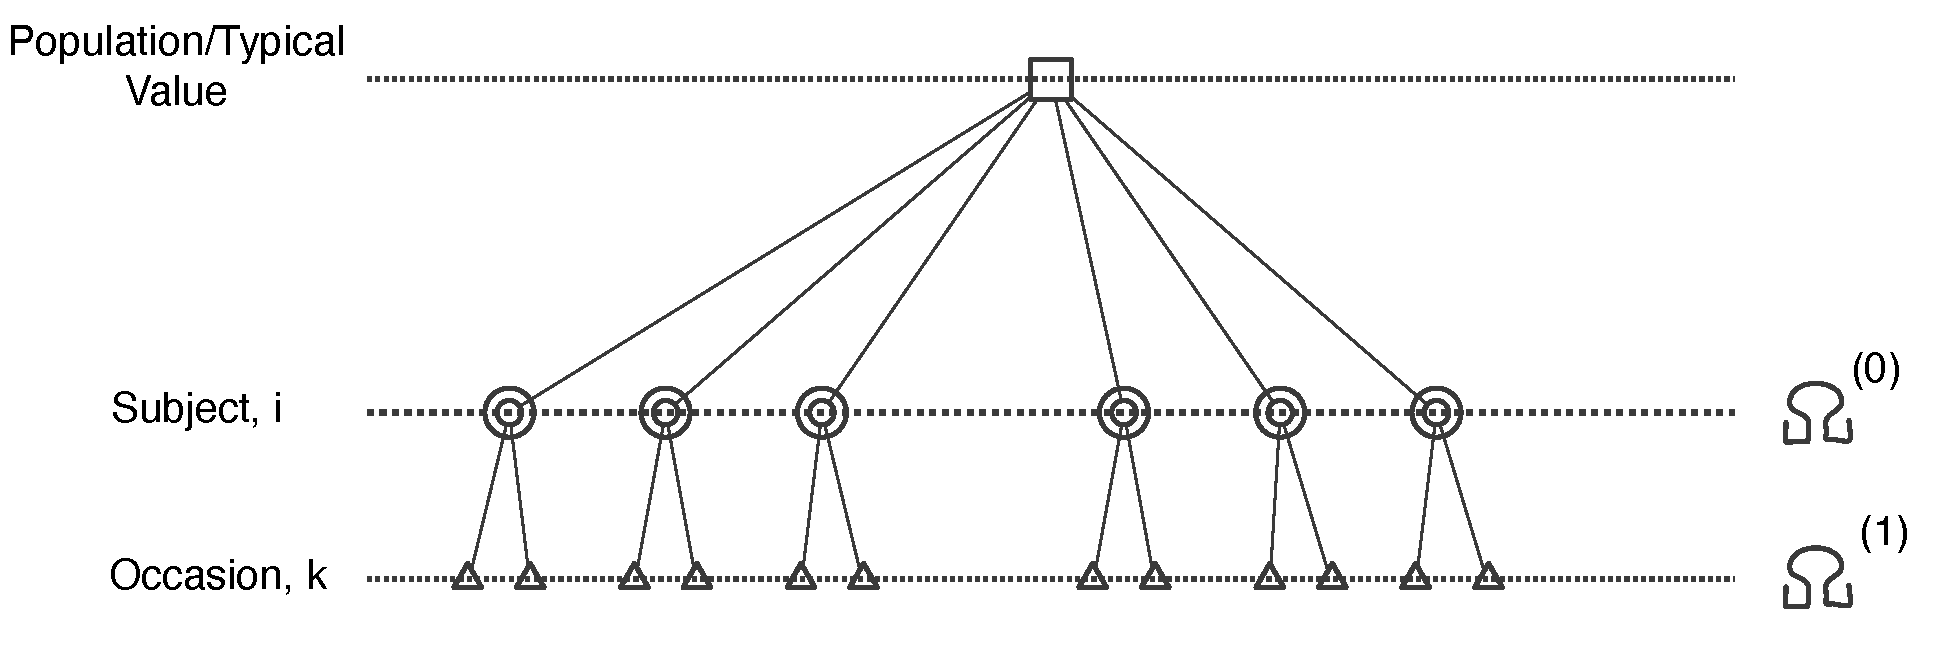
\includegraphics[width=120mm]{pics/IOV_2levels}
\caption{Model with IOV variability level.}
\vspace{-1em}
\label{fig:IOVtree}
\end{figure}


as the following PharmML snippet shows
\lstset{language=XML}
\begin{lstlisting}
            <IndividualParameter symbId="V">
                <ct:VariabilityReference>
                    <ct:SymbRef symbIdRef="iov"/>
                    <ct:RandomEffectMapping>
                        <ct:SymbRef symbIdRef="kappa_V"/>
                    </ct:RandomEffectMapping>
                </ct:VariabilityReference>
                <ct:VariabilityReference>
                    <ct:SymbRef symbIdRef="subject"/>
                    <ct:RandomEffectMapping>
                        <ct:SymbRef symbIdRef="omega_V"/>
                    </ct:RandomEffectMapping>
                </ct:VariabilityReference>
                <Distribution>
                    <ProbOnto name="Normal1">
                        <Parameter name="mean">
                            <ct:Assign>
                                <math:Equation>
                                    <math:Uniop op="log">
                                        <ct:SymbRef symbIdRef="Vpop"/>
                                    </math:Uniop>
                                </math:Equation>
                            </ct:Assign>
                        </Parameter>
                        <Parameter name="stdev">
                            <ct:Assign>
                                <math:Equation>
                                    <math:Binop op="plus">
                                        <ct:SymbRef symbIdRef="omega_V"/>
                                        <ct:SymbRef symbIdRef="kappa_V"/>
                                    </math:Binop>
                                </math:Equation>
                            </ct:Assign>
                        </Parameter>
                    </ProbOnto>
                </Distribution>
            </IndividualParameter>
\end{lstlisting}
The code above illustrates how 
\begin{itemize}
\item 
expressions can be encoded using ProbOnto,
here the $\log(Vpop)$ as the \emph{mean} parameter of the normal distribution.
\item
higher variability levels -- here the IOV -- by mapping of the according variances
to a particular level using the new \xelem{RandomEffectMapping} element. $\omega_V$
is mapped to IIV, $\kappa_V$ is mapped to IOV. Note, that the same information could 
have been implemented using the \xelem{StructuredModel}, but additionally two random 
effects would have to be declared.
\end{itemize}

%%%%%%%%%%%%%%%%%%%%%%%%%%%%%%%%%%%%%%%%%%%%%%%%%%%%%%%%%%%%%%%%%%%%%%
\section{Population parameter -- new}
\label{sec:populationParameter}
Population parameter comes with a flexible structure and can have an 
associated distribution, see Chapter \ref{ch:Bayesian} on Bayesian inference 
and hierarchical models.Two representations are available 
\begin{description} 
\item[Type P1] Equation type
\begin{align*}
\psi_{pop} = H(\beta_i, \eta_i, ...)
\end{align*}
\item[Type P2] Distribution type, i.e. eta-free notation 
\begin{align*}
	& h(\psi_{pop}) \sim Distribution(parameter1, parameter2, ...)
\end{align*}
%	 e.g.
%\begin{align*}
%	& \log(V_{pop}) \sim \mathcal N(\mu_{V_{pop}}, var_{V_{pop}})
%\end{align*}
\end{description}

\begin{note} 
\xelem{PopulationParameter} replaces the \xelem{SimpleParameter} which 
became redundant as the \marginpar{\HandCuffLeft} latter was used so far 
as a population parameter.
\end{note} 

\begin{example}
Using UncertML - from \emph{example3311.xml} model:
\begin{align*}
	lPOP_K \sim \mathcal N\big(lMU_{POP_K}, VAR_{POP_K}\big)
\end{align*}
is encoded in PharmML as
\lstset{language=XML}
\begin{lstlisting}
    <PopulationParameter symbId="lPOP_K">
        <ct:VariabilityReference>
            <ct:SymbRef symbIdRef="pop" blkIdRef="model"/>
        </ct:VariabilityReference>
        <Distribution>
            <UncertML>
                <NormalDistribution xmlns="http://www.uncertml.org/3.0" definition="">
                    <mean>
                        <var varId="lMU_POP_K"/>
                    </mean>
                    <variance>
                        <var varId="VAR_POP_K"/>
                    </variance>
                </NormalDistribution>
            </UncertML>
        </Distribution>
    </PopulationParameter>
\end{lstlisting}
\end{example}

\begin{example}
Using ProbOnto and Type P2 - from fourModels\_hierarchical.xml, \cite{LavielleFourModels:2014},
\begin{align*}
	V_{pop} \sim \mathcal {LN}\big(log(V\!s), gV\big)
\end{align*}
is encoded in PharmML as
\lstset{language=XML}
\begin{lstlisting}
            <PopulationParameter symbId="V_pop">
                <ct:VariabilityReference>
                    <ct:SymbRef blkIdRef="vm1" symbIdRef="pop"/>
                </ct:VariabilityReference>
                <Distribution>
                    <ProbOnto name="LogNormal1">
                        <Parameter name="meanLog">
                            <ct:Assign>
                                <math:Equation>
                                    <math:Uniop op="log">
                                        <ct:SymbRef symbIdRef="Vs"/>
                                    </math:Uniop>
                                </math:Equation>
                            </ct:Assign>
                        </Parameter>
                        <Parameter name="stdevLog">
                            <ct:Assign>
                                <ct:SymbRef symbIdRef="gV"/>
                            </ct:Assign>
                        </Parameter>
                    </ProbOnto>
                </Distribution>
            </PopulationParameter>
\end{lstlisting}
\end{example}

%%%%%%%%%%%%%%%%%%%%%%%%%%%%%%%%%%%%%%%%%%%%%%%%%%%%%%%%%%%%%%%%%%%%%%
\section{Observation model -- {\color{black} \scshape{extended}}}
\label{sec:observationModel}


\subsection{Discrete data models}
The new features are 
\begin{itemize}
\item
Seriously simplified encoding of discrete data models. In \pml versions $\leq$ 0.6 
the implementation of explicit PMF was required for many models due to the lack of 
their coverage in UncertML
\item
All common/relevant parametric distributions and/or their alternative parameterisations 
are supported by ProbOnto, as described in Chapter \ref{ch:ProbOnto}.
\item
Addition of new distributions is straightforward and will be done upon request
\item
An example of ProbOnto use has been shown in section \ref{sec:workingProbOnto}, 
and is shown here with the complete observation model for count data
\begin{itemize}
\item
Type of observed variable -- discrete/count
\item
Model name: NegativeBinomial2
\item
Count variable: $y$
\item
Number of counts: $k$
\item
Probability mass function
\begin{eqnarray}
P(y_{ij} = k; \lambda, \tau) &=& \Bigg[ \frac{\Gamma \big( k + \frac{1}{\tau} \big)}{k! \times \Gamma \big(\frac{1}{\tau} \big)} \Bigg] \times \Bigg( \frac{1}{1 + \tau \times \lambda} \Bigg)^{\frac{1}{\tau}} \times \Bigg(\frac{\lambda}{\frac{1}{\tau} + \lambda} \Bigg)^k \nonumber
\end{eqnarray}
\item
Link function: $\log$
\item
Dispersion parameter, $\tau$
\item
Constant rate parameter $\lambda$, the Poisson 'intensity': $\lambda(t_{ij}, \psi_{ij}) = \lambda_{i}$
\end{itemize}
and reads in PharmML as
\lstset{language=XML}
\begin{lstlisting}
        <ObservationModel blkId="om2">
            <Discrete>
                <CountData>
                    <CountVariable symbId="y"/>
                    <NumberCounts symbId="k"/>
                    
                    <PMF linkFunction="log">
                        <math:LogicBinop op="eq">
                            <ct:SymbRef symbIdRef="y"/>
                            <ct:SymbRef symbIdRef="k"/>
                        </math:LogicBinop>
                        <ProbOnto name="NegativeBinomial2">
                            <Parameter name="rate">
                                <ct:Assign>
                                    <ct:SymbRef blkIdRef="pm1" symbIdRef="lambda"/>
                                </ct:Assign>
                            </Parameter>
                            <Parameter name="overdispersion">
                                <ct:Assign>
                                    <ct:SymbRef blkIdRef="pm1" symbIdRef="tau"/>
                                </ct:Assign>
                            </Parameter>
                        </ProbOnto>
                    </PMF>
                </CountData>
            </Discrete>
        </ObservationModel>
\end{lstlisting}
with \emph{lambda} and \emph{tau} defined in the parameter model, \xatt{pm1}
\end{itemize}


\subsection{Continuous data models}
\label{subsec:contModels}
Available observation model representation has been extended and the available types are
\begin{description} 
\item[Type O1] Structured model 
%(VariabilityReference not mandatory , RLHS required)
\begin{align*}
	u(y) = u(f) + g \times \epsilon \quad [\text{Gaussian if } \epsilon \sim \mathcal N(.,.)]
\end{align*}
is still used with the \xelem{Standard} tag (but comes with extended interpretation 
and allows non-Gaussian residual errors (see the related discussion in section 
\ref{sec:individualParameter}).
\item[Type O2] General model (equation type), unchanged compared to 0.6
%(VariabilityReference not required, LHS transformation optional)
\begin{align*}
	h(y) = H(f, \xi, \epsilon)
\end{align*}

\item[Type O3] ({\color{red} \scshape{NEW}}) Distribution type ($\epsilon$-free notation) 
%(VariabilityReference required, LHS transformation optional)
\begin{align*}
	& u(y)  \sim DistributionName(parameter1, parameter2, ...)
\end{align*}

\end{description}

\begin{table}[ht!]
\setlength{\tabcolsep}{1pt}
\begin{center}
\begin{tabular}{cc}
  \hline
  \hline
\textbf{Type O1} representation  &  \textbf{Type O3} representation \\
  \hline
$Y = C + SD\_ADD \times \epsilon \quad \text{with} \quad \epsilon \sim \mathcal N(0,1)$ \Gape[.4cm][.2cm]{} 
& 
$Y  \sim \mathcal N(C,SD\_ADD)$
\\
  \hline
% \multicolumn{2}{c}{encoding [0,2,0,0,5,0,0,0,0,0]}  \\
%  \hline
  \lstset{language=XML}
\begin{lstlisting}
<Standard symbId="Y">
   <Output>
     <!-- blkIdRef="sm1" -->
     <ct:SymbRef symbIdRef="C"/>
   </Output>
   <ErrorModel>
     <!-- blkIdRef="pm1" -->
     <ct:Assign>
        <ct:SymbRef symbIdRef="SD_ADD"/>
     </ct:Assign>
   </ErrorModel>
   <ResidualError>
      <ct:SymbRef symbIdRef="eps"/>
   </ResidualError>
</Standard>
<!-- declaration of 'eps' omitted -->
\end{lstlisting}
&
\lstset{language=XML}
\begin{lstlisting}
<General symbId="Y">
   <ct:VariabilityReference>
      <ct:SymbRef symbIdRef="residual"/>
   </ct:VariabilityReference>
   <Distribution>
      <ProbOnto name="Normal1">
         <Parameter name="mean">
            <ct:Assign>
               <ct:SymbRef symbIdRef="C"/>
            </ct:Assign>
         </Parameter>
        <Parameter name="stdev">
            <ct:Assign>
               <ct:SymbRef symbIdRef="SD_ADD"/>
            </ct:Assign>
         </Parameter>
      </ProbOnto>
   </Distribution>
</General>
\end{lstlisting}  \\
  \hline
  \end{tabular}
\vspace{-1.5em}
\caption{Comparison of \textit{Type O1} and \textit{Type O3} ($\epsilon$-free) 
representations. For better code readability the \xatt{blkIdRef} attributes have 
been removed.}
\label{tab:typeComparison}
\end{center}
\end{table}


%\subsection{Model overview}
%
%\begin{table}[ht!]
%\setlength{\tabcolsep}{1pt}
%\begin{center}
%\begin{tabular}{cc}
%  \hline
%  \hline
%Individual parameter  & Population parameter \\
%  \hline
%\\
%  \hline
%  \lstset{language=XML}
%\begin{lstlisting}
%
%\end{lstlisting}
%&
%\lstset{language=XML}
%\begin{lstlisting}
%
%\end{lstlisting}  \\
%  \hline
%  \end{tabular}
%\vspace{-1.5em}
%\caption{Compilation of parameter models ...}
%\label{tab:modelCompilation}
%\end{center}
%\end{table}

%%%%%%%%%%%%%%%%%%%%%%%%%%%%%%%%%%%%%%%%%%%%%%%%%%%%%%%%%%%%%%%%%%%%%%
%%%%%%%%%%%%%%%%%%%%%%%%%%%%%%%%%%%%%%%%%%%%%%%%%%%%%%%%%%%%%%%%%%%%%%%
%%%%%%%%%%%%%%%%%%%%%%%%%%%%%%%%%%%%%%%%%%%%%%%%%%%%%%%%%%%%%%%%%%%%%%%
%%%%%%%%%%%%%%%%%%%%%%%%%%%%%%%%%%%%%%%%%%%%%%%%%%%%%%%%%%%%%%%%%%%%%%%
\chapter{Hierarchical model and Bayesian Inference}
\label{ch:Bayesian}

While the detailed Bayesian support is described in the according MDL 
specification proposal, \cite{Chiudinelli2015}, we describe here a few PharmML 
elements, either entirely new, redefined or used in the context of 
hierarchical models and Bayesian inference.

\begin{itemize}
\item 
The \xelem{PopulationParameter} element provides, as indicated in section 
\ref{sec:populationParameter}, the support required for such models.
\item 
ProbOnto provides missing distributions, such as \emph{Inverse-Wishart} 
and other features required. 
\item 
Prior related variability level of any parameter extends its variability 
structure used so far, see Figure \ref{fig:priorVM1}, and 
consequently the extended parameter related variability model for this 
case reads
\lstset{language=XML}
\begin{lstlisting}
        <VariabilityModel blkId="model" type="parameterVariability">
            <Level symbId="pop"/>
            <Level symbId="indiv">
                <ParentLevel>
                    <ct:SymbRef symbIdRef="pop"/>
                </ParentLevel>
            </Level>
        </VariabilityModel>
\end{lstlisting}
\item 
Few basic matrix operators -- such as \emph{inverse},  \emph{transpose}, 
\emph{trace} has been introduced to allow for encoding of certain models, 
see examples in the next section.
\end{itemize}


\begin{figure}[htb!]
\centering
\begin{tabular}{cc}
 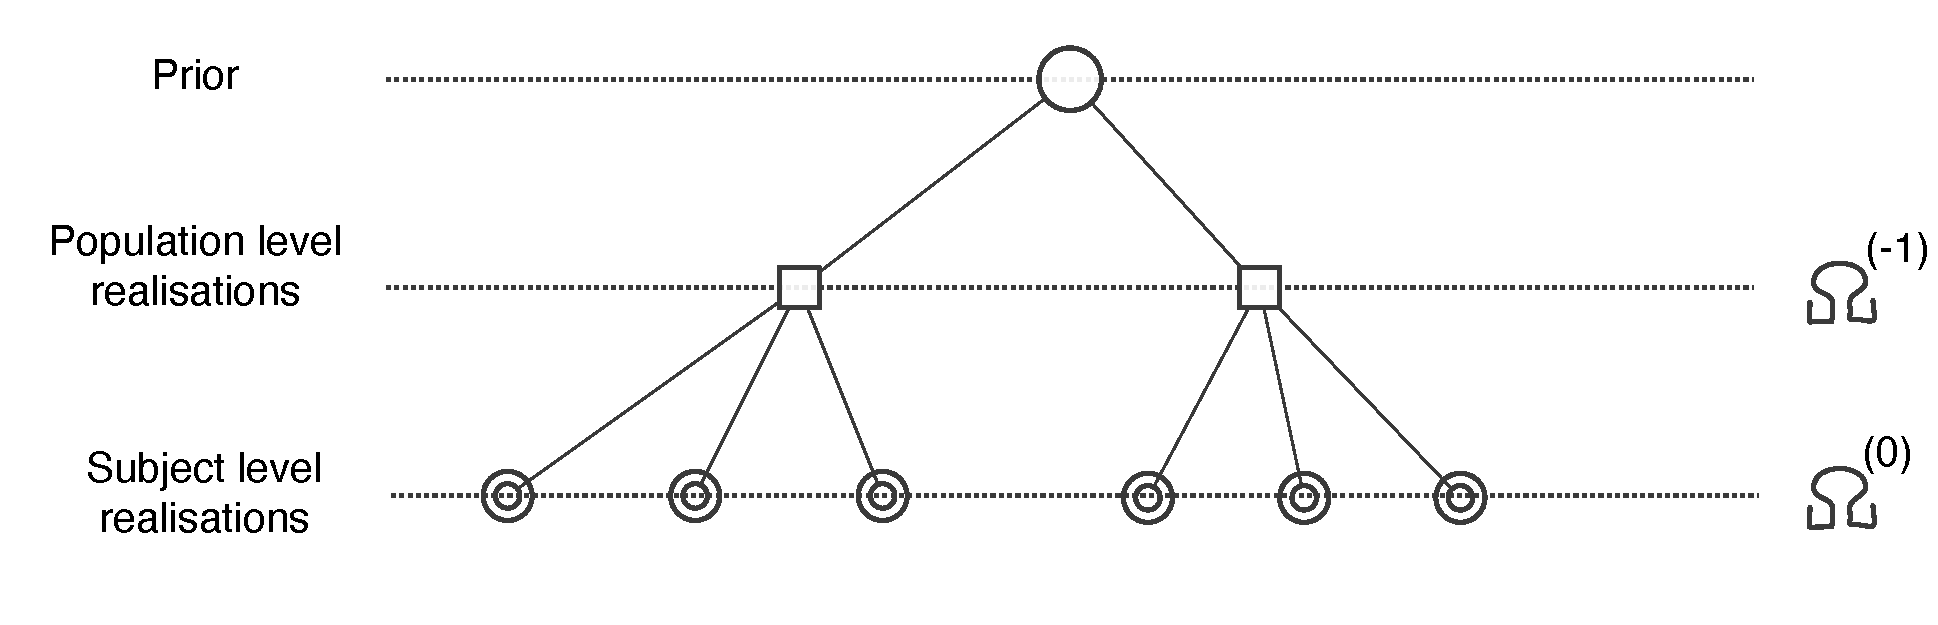
\includegraphics[width=140mm]{pics/IOV0-prior}
\end{tabular}
\caption{Basic variability structure with prior, population and subject levels.}
\label{fig:priorVM1}
\end{figure}

%\begin{figure}[htb!]
%\centering
%\begin{tabular}{cc}
% 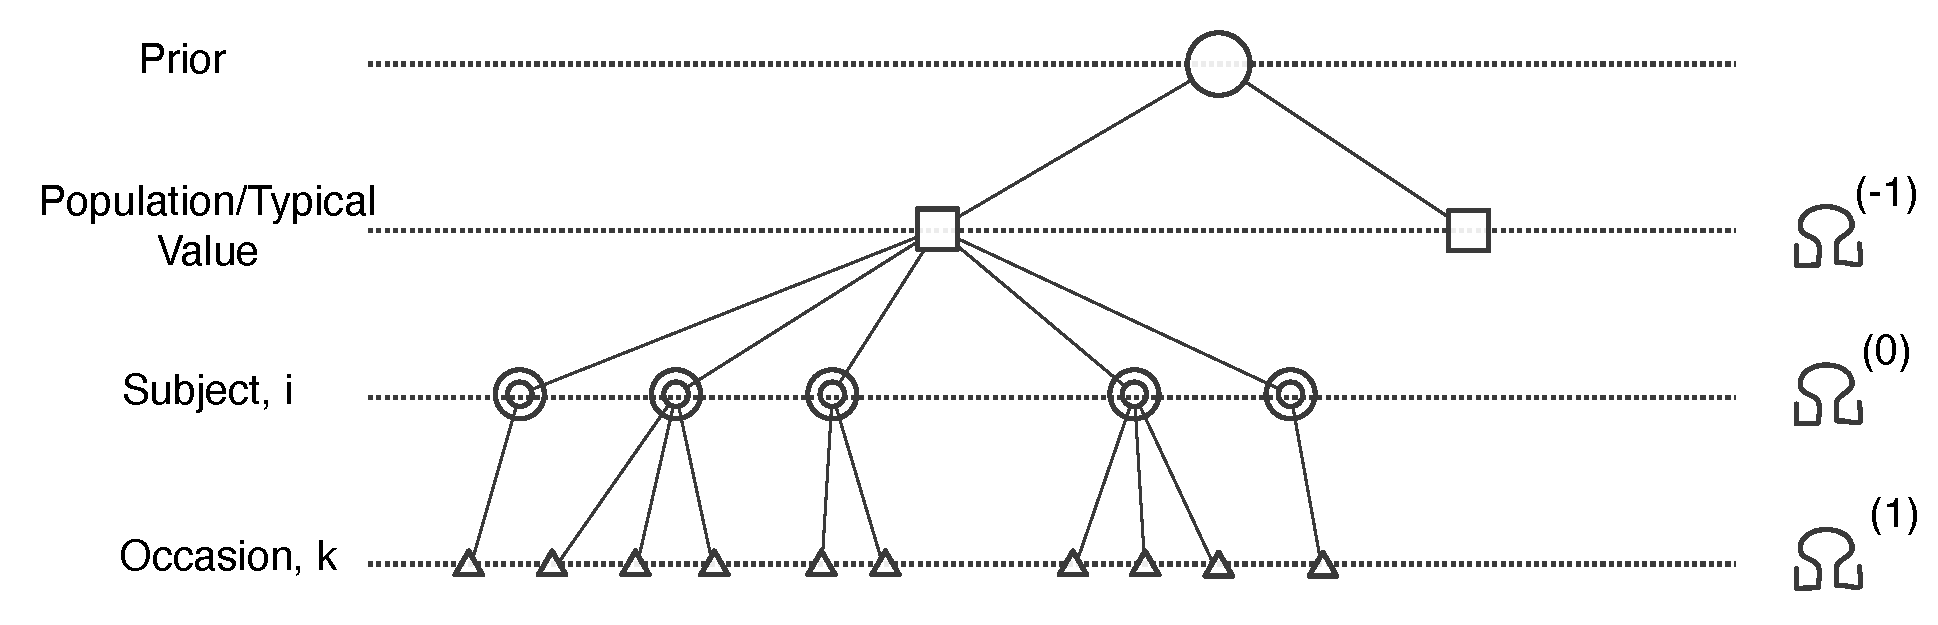
\includegraphics[width=140mm]{pics/IOV_2levels-prior}
%\end{tabular}
%\caption{Variability structure with IOV and priors on population parameters.}
%\label{fig:priorVM2}
%\end{figure}

In section \ref{sec:populationParameter} we have introduced the notation
for population parameters with associated prior distribution. In the following 
we discuss two complete examples, one estimation example as formulated 
typically in winBUGS and a generic hierarchical model, which can be used
for simulation or estimation tasks.

\section{winBUGS \emph{Rats} example}
As an independent example, i.e. not directly related with pharmacometrics,  
we test the schema with a use case from the winBUGS example collection, 
\cite{winBUGSvol1}.
\begin{align*}
Y_{ij} &\sim \mathcal{N}(\alpha_i + \beta_i (x_j - x_{bar}), \tau_c) \\ 
\alpha_i &\sim \mathcal{N}(\alpha_c,\tau_{\alpha}) \\
\beta_i &\sim \mathcal{N}(\beta_c,\tau_{\beta}) 
\end{align*}
in winBUGS code it reads
\lstset{language=MLX}
\begin{lstlisting}
		for( i in 1 : N ) {
			for( j in 1 : T ) {
				Y[i , j] ~ dnorm(mu[i , j],tau.c)
				mu[i , j] <- alpha[i] + beta[i] * (x[j] - xbar)
			}
			alpha[i] ~ dnorm(alpha.c,alpha.tau)
			beta[i] ~ dnorm(beta.c,beta.tau)
		} 
		tau.c~dgamma(0.001,0.001)
		alpha.c ~ dnorm(0.0,1.0E-6)
		alpha.tau ~ dgamma(0.001,0.001)
		beta.c ~ dnorm(0.0,1.0E-6)
		beta.tau ~ dgamma(0.001,0.001)
\end{lstlisting} 
\subparagraph{Observation model} is encoded using the previously introduced 
distribution type, \emph{O3}, section \ref{subsec:contModels}
\lstset{language=XML}
\begin{lstlisting}
        <ObservationModel blkId="om1">
            <ContinuousData>
                <General symbId="Y">
                    <ct:VariabilityReference>
                        <ct:SymbRef blkIdRef="vm2" symbIdRef="residual"/>
                    </ct:VariabilityReference>
                    <Distribution>
                        <ProbOnto name="Normal3">
                            <Parameter name="mean">
                                <ct:Assign>
                                    <ct:SymbRef blkIdRef="pm1" symbIdRef="mu"/>
                                </ct:Assign>
                            </Parameter>
                            <Parameter name="precision">
                                <ct:Assign>
                                    <ct:SymbRef blkIdRef="pm1" symbIdRef="tau.c"/>
                                </ct:Assign>
                            </Parameter>
                        </ProbOnto>
                    </Distribution>
                </General>
            </ContinuousData>
        </ObservationModel>
\end{lstlisting}
with the mean, $\mu$, and another two individual parameters, $\alpha$ and 
$\beta$ encoded next.
\subparagraph{Parameter model} We show only implementation for $\mu$ and $\alpha$ 
($\beta$ is encoded similarily). $\mu$ is an expression but it could have been
implemented directly in the observation model declaration making use of ProbOnto's capability
to assign any expressions to parameters.
\lstset{language=XML}
\begin{lstlisting}
        <IndividualParameter symbId="mu">
            <ct:Assign>
                <Equation xmlns="http://www.pharmml.org/pharmml/0.6/Maths">
                    <Binop op="plus">
                        <ct:SymbRef symbIdRef="alpha"/>
                        <Binop op="times">
                            <ct:SymbRef symbIdRef="beta"/>
                            <Binop op="minus">
                                <ct:SymbRef symbIdRef="x"/>
                                <ct:SymbRef symbIdRef="xbar"/>
                            </Binop>
                        </Binop>
                    </Binop>
                </Equation>
            </ct:Assign>
        </IndividualParameter>
\end{lstlisting}.

\lstset{language=XML}
\begin{lstlisting}
        <IndividualParameter symbId="alpha">
            <ct:VariabilityReference>
                <ct:SymbRef blkIdRef="vm1" symbIdRef="subject"/>
            </ct:VariabilityReference>
            <Distribution>
                <ProbOnto name="Normal3">
                    <Parameter name="mean">
                        <ct:Assign>
                            <ct:SymbRef symbIdRef="alpha.c"/>
                        </ct:Assign>
                    </Parameter>
                    <Parameter name="precision">
                        <ct:Assign>
                            <ct:SymbRef symbIdRef="alpha.tau"/>
                        </ct:Assign>
                    </Parameter>
                </ProbOnto>
            </Distribution>
        </IndividualParameter>
\end{lstlisting}
\subparagraph{Priors} All remaining population parameters $\tau_c$, $\alpha_c$, 
$\alpha_{\tau}$, $\beta_c$, $\beta_{\tau}$ are given \emph{non-informative} 
priors (using Normal or Gamma distribution) and for simplicity we show only the first two.
\lstset{language=XML}
\begin{lstlisting}
        <PopulationParameter symbId="tau.c">
            <ct:VariabilityReference>
                <ct:SymbRef blkIdRef="vm1" symbIdRef="pop"/>
            </ct:VariabilityReference>
            <Distribution>
                <ProbOnto name="Gamma">
                    <Parameter name="shape">
                        <ct:Assign>
                            <ct:Real>0.001</ct:Real>
                        </ct:Assign>
                    </Parameter>
                    <Parameter name="scale">
                        <ct:Assign>
                            <ct:Real>0.001</ct:Real>
                        </ct:Assign>
                    </Parameter>
                </ProbOnto>
            </Distribution>
        </PopulationParameter>
        
        <PopulationParameter symbId="alpha.c">
            <ct:VariabilityReference>
                <ct:SymbRef blkIdRef="vm1" symbIdRef="pop"/>
            </ct:VariabilityReference>
            <Distribution>
                <ProbOnto name="Normal3">
                    <Parameter name="mean">
                        <ct:Assign>
                            <ct:Real>0.0</ct:Real>
                        </ct:Assign>
                    </Parameter>
                    <Parameter name="precision">
                        <ct:Assign>
                            <ct:Real>1.0E-6</ct:Real>
                        </ct:Assign>
                    </Parameter>
                </ProbOnto>
            </Distribution>
        </PopulationParameter>
\end{lstlisting}

\section{PK example}

This example, based on the section 3.3.2 in \cite{Chiudinelli2015}, with correlated
parameters V, k and Vpop, kpop. Here the original model description is used: 
\emph{In this case, the model parameters are not independent random variables 
at both the individual and population level.} It will be useful to present few new 
features such as
\begin{itemize}
\item 
multivariate distributions with parameters, e.g. $\mathcal {MVN}$
\begin{itemize}
\item 
mean as vector
\item 
covariance matrix 
\end{itemize}
\item 
matrix operators, e.g. inverse of a matrix
\item 
new distribution type, $\Gamma (,)$
\end{itemize}

\subsection{Model definition}

\subparagraph{Parameter model}
\begin{align*}
\left(\begin{array}{c} \log(V_j) \\
\log(k_j) \end{array}\right) & \sim
\mathcal {MVN} \left( \Big(\begin{array}{c} \log(V_{pop}) \\ \log(k_{pop}) \end{array}\Big),\Omega_P \right)\\
\log(\tau_{e_j}) &\sim \mathcal N \big(\log(\tau_{pop}),\omega_{\tau}^2\big)
\end{align*}

\subparagraph{Prior distributions}
\begin{align*}
\left(\begin{array}{c} \log(V_{pop}) \\
\log(k_{pop}) \end{array}\right) & \sim
\mathcal {MVN} \left( \Big(\begin{array}{c} \log(\mu_{V_{pop}}) \\ \log(\mu_{k_{pop}}) \end{array}\Big),\Sigma_{P_{pop}} \right)\\
\Omega_P^{-1} &\sim \mathcal {W} (R^{-1},\rho)\\
\omega_{\tau}^{-2} &\sim \Gamma (a_{\omega_{\tau}^2},b_{\omega_{\tau}^2})\\
\tau_{pop} &\sim \Gamma (a_{\tau_{pop}},b_{\tau_{pop}})
\end{align*}

\subparagraph{Structural and observation models}
\begin{align*}
	z_{ij} &\sim \mathcal N(c_{ij},\sigma_{e_j}^2) \\
	c_{ij} &= D/V_j e^{-k_j t_i}
\end{align*}

\subsection{Model implementation}
We will skip the structural and observation models as they don't contribute
any new insights in the discussion relevant to this chapter. Otherwise, we follow 
the winBUGS code as provided, with few following changes 
\begin{itemize}
\item 
removed \xelem{RandomVariable} declaration for \xatt{eps} because of the 
usage of distribution type observation model as defined in the model. 
Accordingly \xelem{Standard} has been replaced by \xelem{General} with 
\xelem{Distribution} tags (see \textit{Type O1}, \textit{Type O3} discussion 
in table \ref{tab:typeComparison}).
\end{itemize}


\paragraph{Parameter model} 
The individual parameters V and k have to be jointly extracted from a 
multivariate distribution. In particular, log(V) and log(k) are the elements 
of a vector, which is distributed as a multivariate Normal with specific 
population mean and covariance matrix describing the inter-individual variability.

In the WinBUGS code, the multivariate Normal requires the vector mean 
and the inverse of covariance matrix as arguments, while in PharmML it has 
been defined with vector mean and covariance matrix.
On the other hand, the individual parameter tau\_e is defined via a univariate 
Normal distribution.

\lstset{language=MLX}
\begin{lstlisting}
	#correlated distribution of V and k of the j-subject
	lP[j,1:2]~dmnorm(lPpop[], TP[ , ])
\end{lstlisting}
in PharmML reads
\lstset{language=XML}
\begin{lstlisting}
            <PopulationParameter symbId="lP">
                <ct:VariabilityReference>
                    <ct:SymbRef symbIdRef="indiv" blkIdRef="model"/>
                </ct:VariabilityReference>
                <Distribution>
                    <ProbOnto name="MultivariateNormal1">
                        <Parameter name="mean">
                            <ct:Assign>
                                <ct:SymbRef symbIdRef="lPOP_P"/>
                            </ct:Assign>
                        </Parameter>
                        <Parameter name="covarianceMatrix">
                            <ct:Assign>
                                <ct:SymbRef symbIdRef="OMEGA_P"/>
                            </ct:Assign>
                        </Parameter>
                    </ProbOnto> 
                </Distribution>
            </PopulationParameter>
\end{lstlisting}
and
\lstset{language=MLX}
\begin{lstlisting}
	#distribution of taue of the j-subject
	ltaue[j]~dnorm(lTpop, Ttau)
	taue[j] <- exp(ltaue[j])
\end{lstlisting}
in PharmML reads
\lstset{language=XML}
\begin{lstlisting}
        <IndividualParameter symbId="TAU">
            <StructuredModel>
                <Transformation type="log"/>
                <LinearCovariate>
                    <PopulationValue>
                        <ct:Assign>
                            <ct:SymbRef symbIdRef="POP_T"/>
                        </ct:Assign>
                    </PopulationValue>
                </LinearCovariate>
                <RandomEffects>
                    <ct:SymbRef symbIdRef="eta_T"/>
                </RandomEffects>
            </StructuredModel>
        </IndividualParameter>
\end{lstlisting}
with implementation of \emph{eta\_T} not shown here as it uses the 
well known \xelem{RandomVariable} element for its encoding.\\
The V and k individual parameters have to be retrieved. The lP vector elements are log(V) and log(k), so the exponential of the lP elements must be computed to obtain V and k.

\lstset{language=MLX}
\begin{lstlisting}
	lV[j] <- lP[j,1]
	V[j] <- exp(lV[j]) 
	lk[j] <- lP[j,2]
	k[j] <- exp(lk[j]) 
\end{lstlisting}
in PharmML reads
\lstset{language=XML}
\begin{lstlisting}
        <IndividualParameter symbId="V">
            <ct:Assign>
                <Equation xmlns="http://www.pharmml.org/pharmml/0.6/Maths">
                    <Uniop op="exp">
                        <ct:VectorSelector>
                            <ct:SymbRef symbIdRef="lP"/>
                            <ct:Cell>
                                <ct:Int>2</ct:Int>
                            </ct:Cell>
                        </ct:VectorSelector>
                    </Uniop>
                </Equation>
            </ct:Assign>
        </IndividualParameter>
        
        <!-- k omitted here -->
\end{lstlisting}

\paragraph{Priors} specification  \\
The prior model on the fixed effect 'tau\_Ppop'
\lstset{language=MLX}
\begin{lstlisting}
	# prior on "THETA"
	tau_Ppop[1:2, 1:2] <- inverse(sigma_Ppop[ , ])
\end{lstlisting}
and requires the definition of the matrix and it reads in PharmML as
\lstset{language=XML}
\begin{lstlisting}
            <PopulationParameter symbId="SIGMA_POP_P">
                <ct:Assign>
                    <ct:Matrix matrixType="Any">
                        <ct:MatrixRow>
                            <ct:RowIndex><ct:Int>1</ct:Int></ct:RowIndex>
                            <ct:Real>1</ct:Real>
                            <ct:Real>0.1</ct:Real>
                            </ct:MatrixRow>
                        <ct:MatrixRow>
                            <ct:RowIndex><ct:Int>2</ct:Int></ct:RowIndex>
                            <ct:Real>0.1</ct:Real>
                            <ct:Real>1</ct:Real>
                        </ct:MatrixRow>
                    </ct:Matrix>
                </ct:Assign>
            </PopulationParameter>
\end{lstlisting}
The vector of the population values
\lstset{language=MLX}
\begin{lstlisting}
	lmu_Ppop[1] <- log(mu_Vpop)
	lmu_Ppop[2] <- log(mu_kpop)
\end{lstlisting}
in PharmML reads
\lstset{language=XML}
\begin{lstlisting}
        <PopulationParameter symbId="lMU_POP_P">
            <ct:Assign>
                <ct:Vector>
                    <ct:VectorElements>
                        <ct:SymbRef symbIdRef="lMU_POP_K"/>
                        <ct:SymbRef symbIdRef="lMU_POP_V"/>
                    </ct:VectorElements>
                </ct:Vector>
            </ct:Assign>
        </PopulationParameter>
        
        <PopulationParameter symbId="lMU_POP_V">
            <ct:Assign>
                <Equation xmlns="http://www.pharmml.org/pharmml/0.6/Maths">
                    <Uniop op="log">
                        <ct:SymbRef symbIdRef="MU_POP_V"/>
                    </Uniop>
                </Equation>
            </ct:Assign>
        </PopulationParameter>
        <!-- with -->        
        <PopulationParameter symbId="MU_POP_V"/>
        <!-- k omitted here -->
\end{lstlisting}
The vector of log of the population parameters Vpop and kpop is a-priori distributed as a multivariate Normal with user-defined vector mean and covariance matrix, reported above.
\lstset{language=MLX}
\begin{lstlisting}
	lPpop[1:2]~dmnorm(lmu_Ppop[], tau_Ppop[ , ])
\end{lstlisting}
in PharmML reads

\lstset{language=XML}
\begin{lstlisting}
        <PopulationParameter symbId="lPOP_P">
            <ct:VariabilityReference>
                <ct:SymbRef symbIdRef="pop" blkIdRef="model"/>
            </ct:VariabilityReference>
            <Distribution>
                <ProbOnto name="MultivariateNormal1">
                    <Parameter name="mean">
                        <ct:Assign>
                            <ct:SymbRef symbIdRef="lMU_POP_P"/>
                        </ct:Assign>
                    </Parameter>
                    <Parameter name="covarianceMatrix">
                        <ct:Assign>
                            <ct:SymbRef symbIdRef="SIGMA_POP_P"/>
                        </ct:Assign>
                    </Parameter>
                </ProbOnto>
            </Distribution>
        </PopulationParameter>
\end{lstlisting}
with the according covariance matrix \emph{SIGMA\_POP\_P} defined above.

The inverse of the covariance matrix \emph{OMEGA\_P} is distributed as a Wishart with given parameters R and rho (not reported). A different parametrization has been used in WinBUGS (in which the inverse of R is required) and PharmML (in which the Wishart1 distribution enables the use of the R matrix)
\lstset{language=MLX}
\begin{lstlisting}
	# prior on inverse of "OMEGA"
	Rinv[1:2,1:2] <- inverse(R[,])
	TP[1:2,1:2]~dwish(Rinv[ , ], rho)
\end{lstlisting}
in PharmML reads
\lstset{language=XML}
\begin{lstlisting}
        <PopulationParameter symbId="OMEGA_P">
            <ct:Assign>
                <Equation xmlns="http://www.pharmml.org/pharmml/0.6/Maths">
                    <MatrixUniop op="inverse">
                        <ct:SymbRef symbIdRef="invOMEGA_P"/>
                    </MatrixUniop>
                </Equation>
            </ct:Assign>
        </PopulationParameter>
        
        <PopulationParameter symbId="invOMEGA_P">
            <ct:VariabilityReference>
                <ct:SymbRef symbIdRef="pri" blkIdRef="model"/>
            </ct:VariabilityReference>
            <Distribution>
                <ProbOnto name="Wishart1">
                    <Parameter name="scaleMatrix">
                        <ct:Assign>
                            <ct:SymbRef symbIdRef="rho"/>
                        </ct:Assign>
                    </Parameter>
                    <Parameter name="degreesOfFreedom">
                        <ct:Assign>
                            <ct:SymbRef symbIdRef="R"/>
                        </ct:Assign>
                    </Parameter>
                </ProbOnto>
            </Distribution>
        </PopulationParameter>
\end{lstlisting}
The inverse of the variance of \emph{eta\_T} (\emph{OMEGA\_T}) is a-priori distributed as a Gamma with user-defined parameters.
\lstset{language=MLX}
\begin{lstlisting}
	Ttau~dgamma(a_omega_tau, b_omega_tau)
\end{lstlisting}
in PharmML reads
\lstset{language=XML}
\begin{lstlisting}
        <PopulationParameter symbId="TAU_T">
            <ct:VariabilityReference>
                <ct:SymbRef symbIdRef="pri" blkIdRef="model"/>
            </ct:VariabilityReference>
            <Distribution>
                <ProbOnto name="Gamma">
                    <Parameter name="shape">
                        <ct:Assign>
                            <ct:SymbRef symbIdRef="a_OMEGA_T"/>
                        </ct:Assign>
                    </Parameter>
                    <Parameter name="scale">
                        <ct:Assign>
                            <ct:SymbRef symbIdRef="b_OMEGA_T"/>
                        </ct:Assign>
                    </Parameter>
                </ProbOnto>
            </Distribution>
        </PopulationParameter>
        
        <PopulationParameter symbId="OMEGA_T">
            <ct:Assign>
                <Equation xmlns="http://www.pharmml.org/pharmml/0.6/Maths">
                    <Binop op="divide">
                        <ct:Real>1</ct:Real>
                        <ct:SymbRef symbIdRef="TAU_T"/>
                    </Binop>
                </Equation>
            </ct:Assign>
        </PopulationParameter>
\end{lstlisting}
\emph{POP\_T} is a-priori distributed as a Gamma with user-defined parameters.
\lstset{language=MLX}
\begin{lstlisting}
	# prior on "SIGMA"
	Tpop~dgamma(a_taupop, b_taupop)
	lTpop <- log(Tpop)
\end{lstlisting}
in PharmML reads
\lstset{language=XML}
\begin{lstlisting}
        <PopulationParameter symbId="POP_T">
            <ct:VariabilityReference>
                <ct:SymbRef symbIdRef="pri" blkIdRef="model"/>
            </ct:VariabilityReference>
            <Distribution>
                <ProbOnto name="Gamma">
                    <Parameter name="shape">
                        <ct:Assign>
                            <ct:SymbRef symbIdRef="a_POP_T"/>
                        </ct:Assign>
                    </Parameter>
                    <Parameter name="scale">
                        <ct:Assign>
                            <ct:SymbRef symbIdRef="b_POP_T"/>
                        </ct:Assign>
                    </Parameter>
                </ProbOnto>
            </Distribution>
        </PopulationParameter>
\end{lstlisting}



The structural model is a standard algebraic equations and its implementation
will not be shown here. The Observation model on the other hand is implemented
using the distribution model and read in PharmML:
\lstset{language=XML}
\begin{lstlisting}
        <General symbId="C">
            <ct:VariabilityReference>
                <ct:SymbRef blkIdRef="resErrorModel" symbIdRef="residual"/>
            </ct:VariabilityReference>
            <Distribution>
                <ProbOnto name="Normal2">
                    <Parameter name="mean">
                        <ct:Assign>
                            <ct:SymbRef blkIdRef="sm1" symbIdRef="C"/>
                        </ct:Assign>
                    </Parameter>
                    <Parameter name="var">
                        <ct:Assign>
                            <ct:SymbRef symbIdRef="sigmaSquare"/>
                        </ct:Assign>
                    </Parameter>
                </ProbOnto>
            </Distribution>
        </General>
\end{lstlisting}
with
\lstset{language=XML}
\begin{lstlisting}
        <IndividualParameter symbId="sigmaSquare">
            <ct:Assign>
                <Equation xmlns="http://www.pharmml.org/pharmml/0.6/Maths">
                    <Uniop op="sqrt">
                        <Binop op="divide">
                            <ct:Real>1</ct:Real>
                            <ct:SymbRef symbIdRef="TAU"/>
                        </Binop>
                    </Uniop>
                </Equation>
            </ct:Assign>
        </IndividualParameter>
\end{lstlisting}
declared in parameter model, \xatt{pm1}.

\section{Hierarchical model example}
The following model has been proposed, \cite{LavielleFourModels:2014},
to test the capabilities of the DDMoRe platform with respect to the encoding of
hierarchical models, encoded here in MLXTRAN
\lstset{language=MLX}
\begin{lstlisting}
    [LONGITUDINAL]
    input = {V, k, b}
    EQUATION:
    D=100
    f = D/V*exp(-k*t)
    DEFINITION:
    y = {distribution=normal, prediction=f, sd=b*f}

    [INDIVIDUAL]
    input = {V_pop, omega_V, w, w_pop}
    EQUATION:
    V_pred = V_pop*(w/w_pop)
    DEFINITION:
    V = {distribution=logNormal, prediction=V_pred, sd=omega_V}

    [COVARIATE]
    input = {w_pop, omega_w}
    DEFINITION:
    w = {distribution=normal, mean=w_pop, sd=omega_w}

    [POPULATION]
    input = {ws, gw, Vs, gV}
    DEFINITION:
    w_pop = {distribution=normal, mean=ws, sd=gw}
    V_pop = {distribution=logNormal, mean=log(Vs), sd=gV}
\end{lstlisting}
In the following we will show only the relevant for this chapter model elements.
\paragraph{Observation model}
\begin{align*}
 y \sim \mathcal N(f,b f)
\end{align*}
reads in PharmML
\lstset{language=XML}
\begin{lstlisting}
    <General symbId="y">
        <ct:VariabilityReference>
            <ct:SymbRef blkIdRef="vm2" symbIdRef="resErr"/>
        </ct:VariabilityReference>
        <Distribution>
            <ProbOnto name="Normal1">
                <Parameter name="mean">
                    <ct:Assign>
                        <ct:SymbRef blkIdRef="sm1" symbIdRef="f"/>
                    </ct:Assign>
                </Parameter>
                <Parameter name="stdev">
                    <ct:Assign>
                        <math:Equation>
                            <math:Binop op="times">
                                <ct:SymbRef blkIdRef="pm1" symbIdRef="b"/>
                                <ct:SymbRef blkIdRef="sm1" symbIdRef="f"/>
                            </math:Binop>
                        </math:Equation>
                    </ct:Assign>
                </Parameter>
            </ProbOnto>
        </Distribution>
    </General>
\end{lstlisting}
Note the encoding of expressions in the second parameter of the normal distribution
easily done when using ProbOnto, was not possible with UncertML.
\paragraph{Individual parameter model} 
\begin{align*}
 V \sim \mathcal {LN}(V_{pred}, \omega_V) \quad \text{with} \quad V_{pred}=V_{pop} (w/w_{pop})
\end{align*}
reads in PharmML:
\lstset{language=XML}
\begin{lstlisting}
    <IndividualParameter symbId="V">
        <ct:VariabilityReference>
            <ct:SymbRef blkIdRef="vm1" symbIdRef="indiv"/>
        </ct:VariabilityReference>
        <Distribution>
            <ProbOnto name="LogNormal1">
                <Parameter name="meanLog">
                    <ct:Assign>
                        <ct:SymbRef symbIdRef="V_pred"/>
                    </ct:Assign>
                </Parameter>
                <Parameter name="stdevLog">
                    <ct:Assign>
                        <ct:SymbRef symbIdRef="omega_V"/>
                    </ct:Assign>
                </Parameter>
            </ProbOnto>
        </Distribution>
    </IndividualParameter>

    <!-- V_pred = V_pop*(w/w_pop) -->
    <PopulationParameter symbId="V_pred">
        <ct:Assign>
            <math:Equation>
                <math:Binop op="times">
                    <ct:SymbRef symbIdRef="V_pop"/>
                    <math:Binop op="divide">
                        <ct:SymbRef blkIdRef="cm1" symbIdRef="w"/>
                        <ct:SymbRef symbIdRef="w_pop"/>
                    </math:Binop>
                </math:Binop>
            </math:Equation>
        </ct:Assign>
    </PopulationParameter>
\end{lstlisting}
\paragraph{Covariate model} describes the distribution of body weight
\begin{align*}
 w \sim \mathcal {N}(w_{pop}, \omega_w)
\end{align*}
can be encoded as
\lstset{language=XML}
\begin{lstlisting}
    <CovariateModel blkId="cm1">
        <Covariate symbId="w">
            <Continuous>
                <Distribution>
                    <ProbOnto name="Normal1">
                        <Parameter name="mean">
                            <ct:Assign>
                                <ct:SymbRef blkIdRef="pm1" symbIdRef="w_pop"/>
                            </ct:Assign>
                        </Parameter>
                        <Parameter name="stdev">
                            <ct:Assign>
                                <ct:SymbRef blkIdRef="pm1" symbIdRef="omega_w"/>
                            </ct:Assign>
                        </Parameter>
                    </ProbOnto>
                </Distribution>
            </Continuous>
        </Covariate>
    </CovariateModel>
\end{lstlisting}
Note, that the population parameters used in the covariate model are 
defined in the parameter model, \xatt{pm1}, as the next code snippet will show.
\paragraph{Population parameters} of the model covariate model 
\begin{align*}
 w_{pop} \sim \mathcal {N}(ws, gw)
\end{align*}
and
\begin{align*}
 V_{pop} \sim \mathcal {LN}\big(\log(V\!s), gV\big)
\end{align*}
are encode as
\lstset{language=XML}
\begin{lstlisting}
    <!-- w_pop = {distribution=normal, mean=ws, sd=gw} -->
    <PopulationParameter symbId="w_pop">
        <ct:VariabilityReference>
            <ct:SymbRef blkIdRef="vm1" symbIdRef="pop"/>
        </ct:VariabilityReference>
        <Distribution>
            <ProbOnto name="Normal1">
                <Parameter name="mean">
                    <ct:Assign>
                        <ct:SymbRef symbIdRef="ws"/>
                    </ct:Assign>
                </Parameter>
                <Parameter name="stdev">
                    <ct:Assign>
                        <ct:SymbRef symbIdRef="gw"/>
                    </ct:Assign>
                </Parameter>
            </ProbOnto>
        </Distribution>
    </PopulationParameter>

    <!-- V_pop = {distribution=logNormal, mean=log(Vs), sd=gV} -->
    <PopulationParameter symbId="V_pop">
        <ct:VariabilityReference>
            <ct:SymbRef blkIdRef="vm1" symbIdRef="pop"/>
        </ct:VariabilityReference>
        <Distribution>
            <ProbOnto name="LogNormal1">
                <Parameter name="meanLog">
                    <ct:Assign>
                        <math:Equation>
                            <math:Uniop op="log">
                                <ct:SymbRef symbIdRef="Vs"/>
                            </math:Uniop>
                        </math:Equation>
                    </ct:Assign>
                </Parameter>
                <Parameter name="stdevLog">
                    <ct:Assign>
                        <ct:SymbRef symbIdRef="gV"/>
                    </ct:Assign>
                </Parameter>
            </ProbOnto>
        </Distribution>
    </PopulationParameter>
\end{lstlisting}


%\section{To-do}
%So far, regarding Bayesian inference and hierarchical models, the intention 
%was directed towards model definition but the mapping to the underlying dataset 
%is not fully defined. While the typical dosing, observation, covariate datasets as 
%use by Monolix or NONMEM can be satisfactory mapped to the model definition 
%in PharmML, winBUGS uses different data format and its mapping requires more
%testing.

%%%%%%%%%%%%%%%%%%%%%%%%%%%%%%%%%%%%%%%%%%%%%%%%%%%%%%%%%%%%%%%%%%%%%%
%%%%%%%%%%%%%%%%%%%%%%%%%%%%%%%%%%%%%%%%%%%%%%%%%%%%%%%%%%%%%%%%%%%%%%%
%%%%%%%%%%%%%%%%%%%%%%%%%%%%%%%%%%%%%%%%%%%%%%%%%%%%%%%%%%%%%%%%%%%%%%%
%%%%%%%%%%%%%%%%%%%%%%%%%%%%%%%%%%%%%%%%%%%%%%%%%%%%%%%%%%%%%%%%%%%%%%%
\chapter{Design -- redesigned}
\label{ch:Design}

%%%%%%%%%%%%%%%%%%%%%%%%%%%%%%%%%%%%%%%%%%%%%%%%%%%%%%%%%%%%%%%%%%%%%%
\section{Design in PharmML $\leq$ 0.6}
Since version 0.2 PharmML was using SDM-XML, a CDISC standard \cite{CDISC:2011a}, 
based trial design. With the beginning of the activities of a group working on trial design
for MDL it became clear that this structure is insufficient and had to be reorganised and 
redesigned, see figure \ref{fig:Flowchart07}. The main reasons are 
\begin{itemize}
\item
CDISC based design is missing many elements, the most important ones being 
the observations and design spaces. Although the former were supported in 
PharmML, their implementation not only had to be done in \xelem{ModellingSteps} 
section but it also lacked the connectivity to study arms.
\item
A number of typical design features, such as arm size, number of arms, total size,
number of samples, number of times, cost function, total cost, was not accounted for.
\item
The rigid structure with epochs/cells/segment was unfamiliar to modellers 
who need a more flexible arm based structure.
\item
Required specifically for optimal design, the re-definition of covariate 
model, required for covariates to be optimised, was not supported in the CDISC 
based structure.
\item
Design elements were spread over two sections, \xelem{TrialDesign} and \xelem{ModellingSteps}
which created an inconsistent structure.
\item
The specification of external datasets, located in \xelem{ModellingSteps}, as the source 
for design belongs to trial design section.
\item
\xelem{ModellingSteps} section should contain only task description.
%- Separation between model-design-tasks required - in Steps only task description - with 2 new elements
\item
The lack of compatibility with the new MDL design proposal -- translation would be 
very hard to achieve given such two different structures.
\end{itemize}
The new design/trial design structure addresses the above issues and 
because it was developed with both MDL and PharmML in mind, it promises 
a very high \marginpar{\HandCuffLeft} degree of compatibility between 
these two languages -- to be verified during the coming months. 


%%%%%%%%%%%%%%%%%%%%%%%%%%%%%%%%%%%%%%%%%%%%%%%%%%%%%%%%%%%%%%%%%%%%%%
\section{Modifications and extensions}
The new trial design structure consists of
\begin{itemize}
\item
Core structure based on the design elements developed for MDL, \cite{Commets2015, CommetsExamples2015}.
\item
Additional features available in PharmML since 0.2.1 such as individual 
observations, dosing, covariates.
\end{itemize}
While the detailed design is described in the according MDL specification proposal, 
\cite{Commets2015}, the comparison on the following pages visualises the changes
and differences. In the left column on page \pageref{miniPage:comparison}, the PharmML 
$\leq$ 0.6 design elements are shown, distributed
over two sections, \xelem{TrialDesign} and \xelem{ModellingSteps}. 
On the right, a detailed list of current elements available for the trial design is given.

All examples provided in the 'Modelling Description Language. Design 
elements - Examples', \cite{CommetsExamples2015}, and all explicit design 
based examples from the PharmML specification, \cite{Pharmml_06}, have 
been successfully implemented.

\newpage
\begin{figure}[htb!]
\centering
  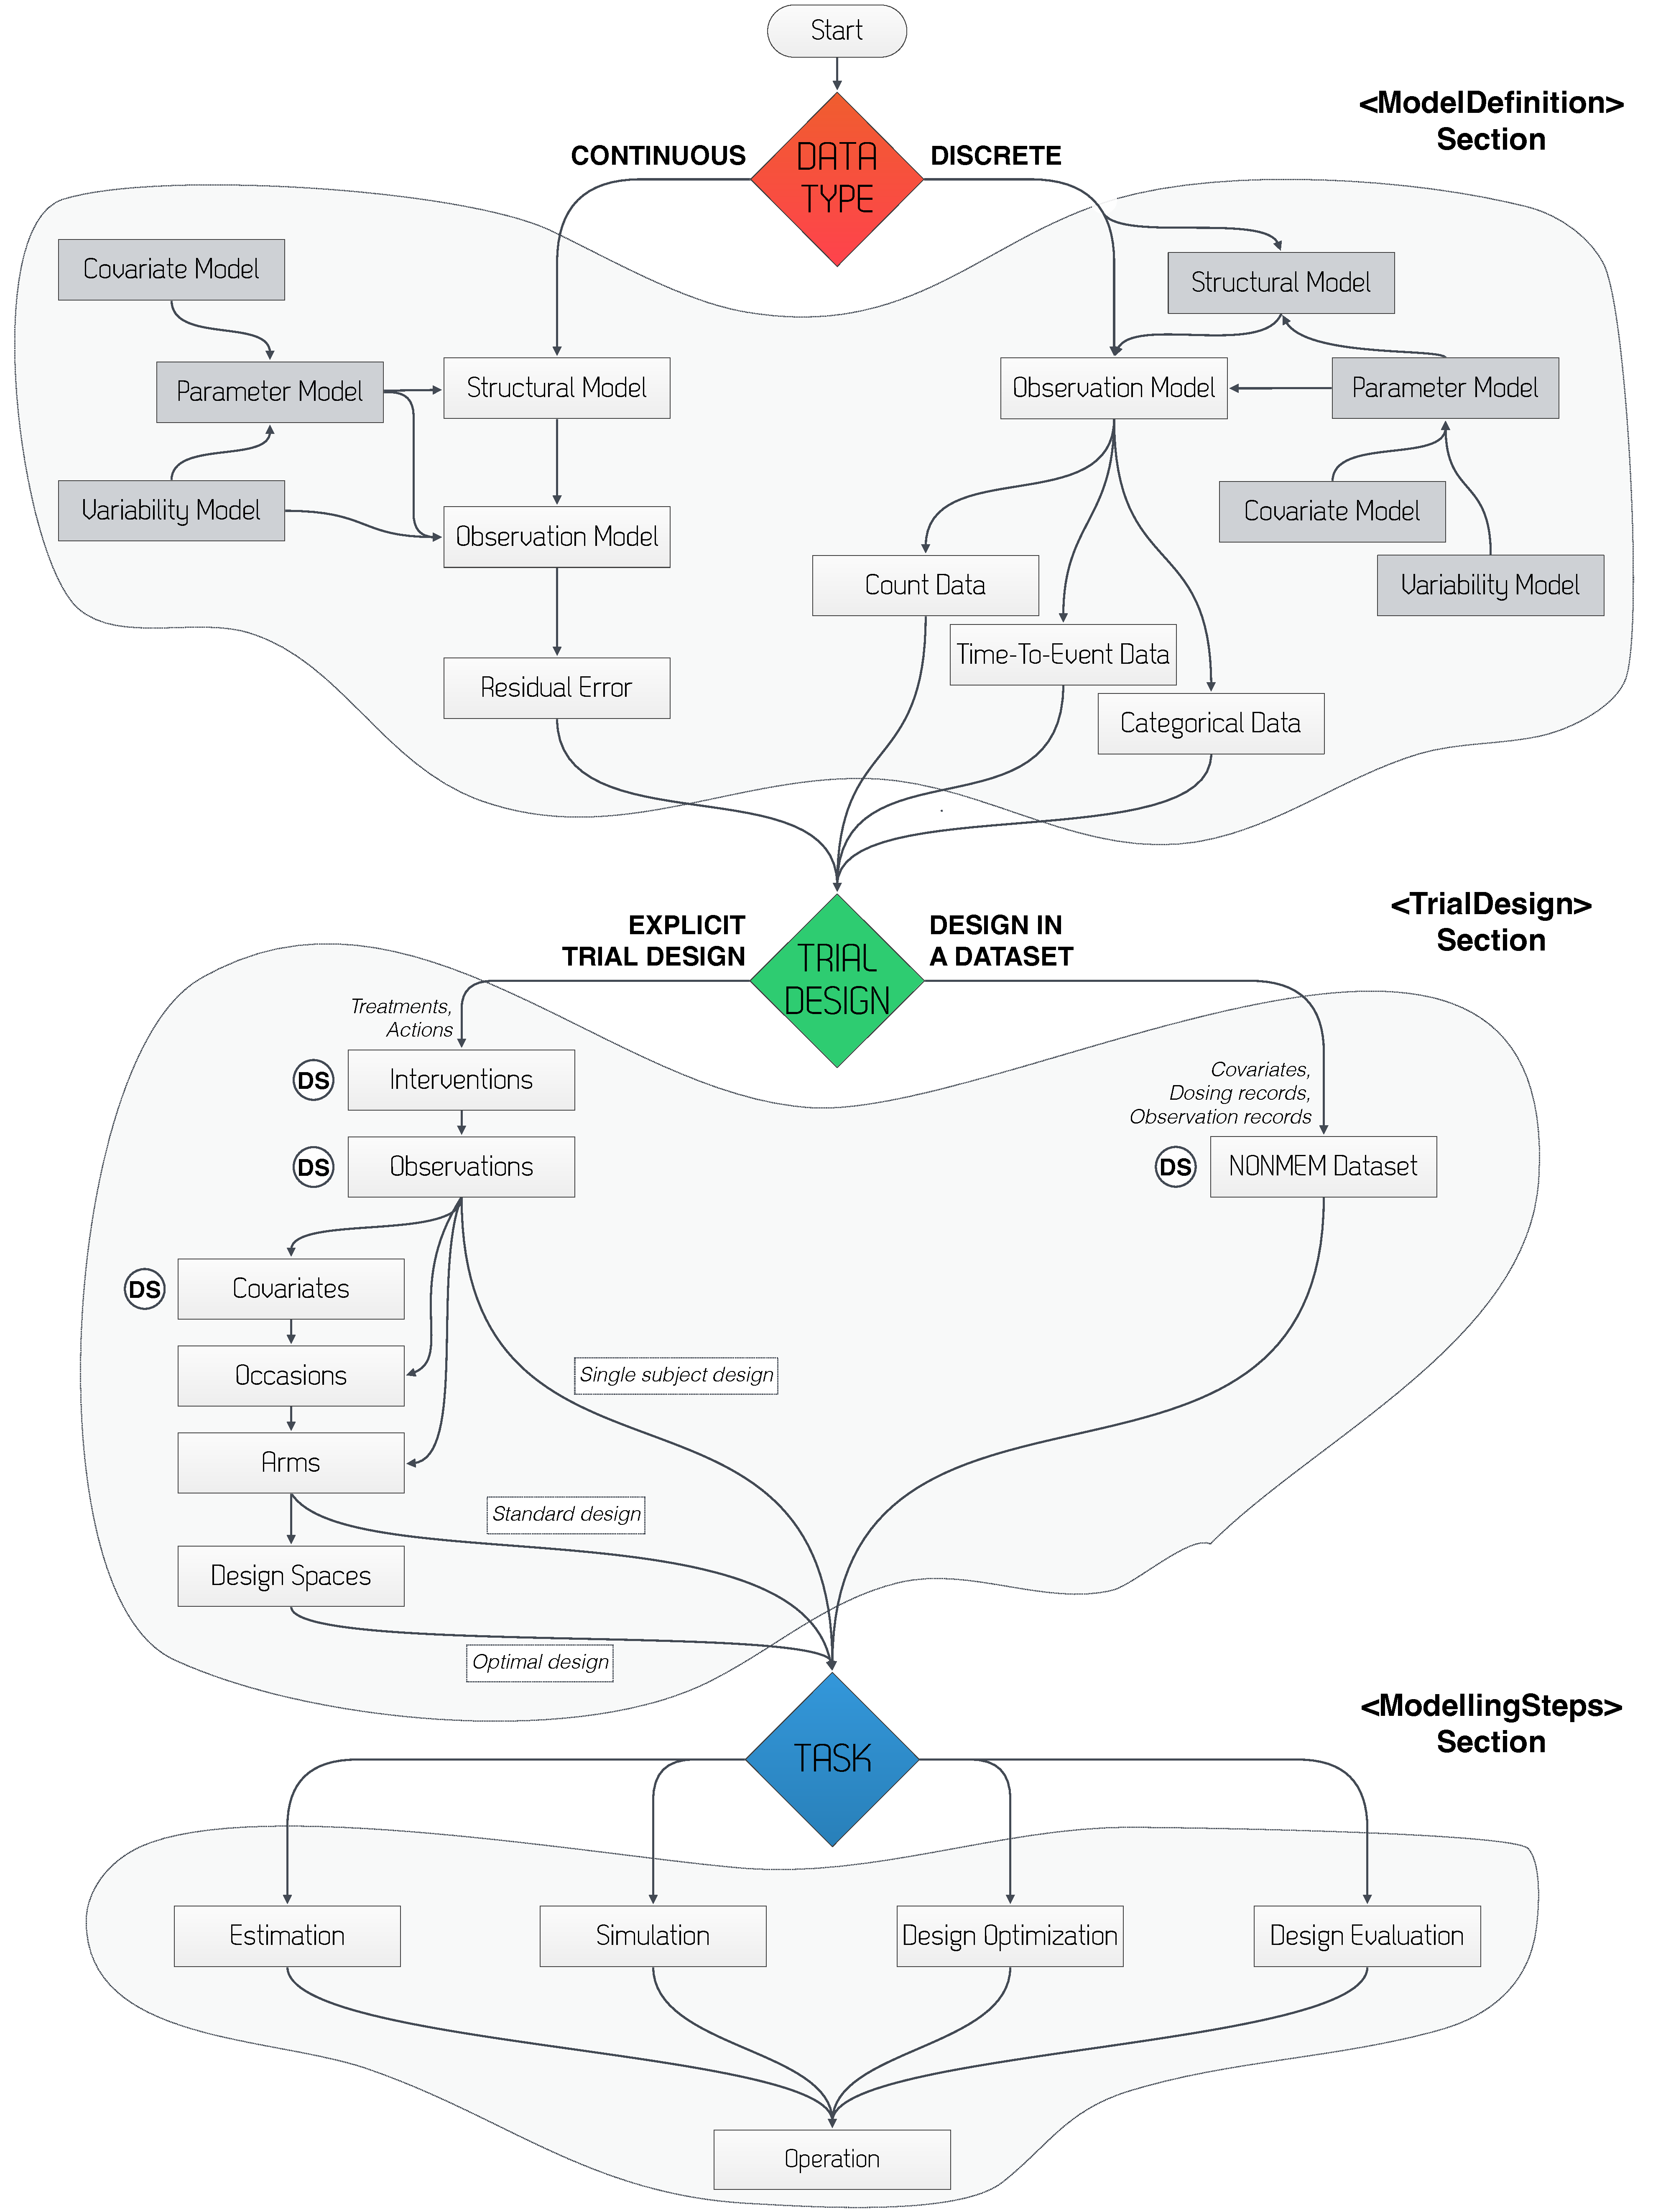
\includegraphics[width=165mm]{pics/Flowchart07}
 \caption{Working with PharmML -- a schema showing three essential decision points: 
 (A) the type of data (continuous and discrete), (B) the source of the study design and 
 data (Monolix/NONMEM dataset or \xelem{TrialDesign}) and finally (C) the task type 
 (for now only simulation and estimation tasks are fully supported, the design related 
 tasks are under construction). \textbf{Note} that in comparison to 0.6 version, \cite{Pharmml_06}, 
 all data and design elements are located in the \xelem{TrialDesign} section while the last 
 section, \xelem{ModellingSteps}, carries only tasks related information.}
 \label{fig:Flowchart07}
\end{figure}

\newpage

%\LTcapwidth=\textwidth
%\begin{center}
%\renewcommand{\arraystretch}{1.1}%
%\begin{longtable}{llcccc}
%  \hline
%  \hline
%0.6 & 0.7\\
%%\multicolumn{1}{c}{0.2}			& risation		&  3.0			& 1.4		& 4.3	& 7.3 \\
%  \hline
%
%  \hline \\
%\caption{Structure comparison of the trial design related features.}
%\label{Tab:NewOldDesign}
%%\vspace{-3.5em}
%\end{longtable}
%\end{center}


%%%%% LEFT PAGE %%%%%
\begin{minipage}{0.35\textwidth}
\small
\centering 
\pml $\le$ 0.6\\
{\color{red} \scshape{\xelem{TrialDesign}}}
\begin{flushleft} 
\begin{itemize}
\item 
Structure
\begin{itemize}
\item
Arm
\item
Cell
\item
Epoch
\item
Segment
\item
Activity
\begin{itemize}
\item
Bolus
\item
Infusion
\item
Washout
\item
Lookup table
\item
Epoch Ref/Period
\end{itemize}
\end{itemize}
\item
Population
\begin{itemize}
\item
Arm memberships \& covariates
\item
Demographics
\end{itemize}
\item 
Individual Dosing
\end{itemize}
\vspace{2em}
\end{flushleft}
\centering 
{\color{red} \scshape{\xelem{ModellingSteps}}}
\begin{flushleft} 
\begin{itemize}
\item 
\textbf{ExternalDataSet}
\item 
Simulation Step
\begin{itemize}
\item 
\textbf{Observations}
\item 
Operation
\end{itemize}
\item 
Estimation Step
\begin{itemize}
\item 
\textbf{ObjectiveData}
\item 
Parameter Estimation
\item 
Operation
\end{itemize}
\item 
Step dependencies
\end{itemize}
\end{flushleft}
\end{minipage}
%%%%% RIGHT PAGE %%%%%
\begin{minipage}{0.6\textwidth}
\small
\centering 
\pml 0.7\\
{\color{red} \scshape{\xelem{TrialDesign}}}
\begin{flushright}
\begin{itemize}
\item 
ExternalDataSet
\item 
Interventions
\begin{itemize}
\item 
Administration
\begin{itemize}
\item 
InterventionRef
\item
Bolus
\item
Infusion
\end{itemize}
\item 
IndividualAdministration
\item 
Action -- Washout
\begin{itemize}
\item 
full reset
\item 
variable-wise
\end{itemize}
\item
InterventionsCombination
\end{itemize}
\item 
Observations
\begin{itemize}
\item 
LookupTable 
\item 
IndividualObservations
\item 
Observation
\item 
ObservationsCombination
\end{itemize}
\item 
Covariates
\begin{itemize}
\item 
CovariateModel
\begin{itemize}
\item
Categorical/Category: Probability, OccasionRef, InterventionRef, InterventionSequence
\end{itemize}
\item 
IndividualCovariates
\end{itemize}
\item 
Occasions/OccasionList
\begin{itemize}
\item 
VariabilityReference
\item 
Occasion
\end{itemize}
\item 
Arms
\begin{itemize}
\item 
Simple elements: ArmSize, CostFunction, NumberArms, NumberSamples, NumberTimes, SameTimes, TotalCost, TotalSize
\item 
Arm
\begin{itemize}
\item 
Simple elements: ArmSize, NumberSamples, NumberTimes, SameTimes
\item 
InterventionSequence/List
\item 
ObservationSequence/List
\item 
OccasionSequence/List
\end{itemize}
\end{itemize}
\item 
DesignSpaces
\begin{itemize}
\item 
References: InterventionRef, ObservationRef, ArmRef, SymbRef, CovariateModelRef \& CovariateRef
\item 
Simple elements: ArmSize, DoseAmount, DosingTimes, Duration, NumberArms, NumberSamples, NumberTimes, SampleTimes
\end{itemize}
\end{itemize}
\end{flushright}
{\color{red} \scshape{\xelem{ModellingSteps}}}
\begin{flushleft} 
\begin{itemize}
\item 
Simulation Step w. Operation
\item 
Estimation Step w. Parameter Estimation \& Operation
\item 
Design Optimization Step -- {\color{darkgreen} \scshape{under construction}} 
\item 
Design Evaluation Step -- {\color{darkgreen} \scshape{under construction}}
\item 
Step dependencies
\end{itemize}
\end{flushleft}
\label{miniPage:comparison}
\end{minipage}



%%%%%%%%%%%%%%%%%%%%%%%%%%%%%%%%%%%%%%%%%%%%%%%%%%%%%%%%%%%%%%%%%%%%%%
\section{Selected features}
The trial design structure, although intuitive and relatively easy to learn,
is quite complex. The reader is referred to the original specification 
and example documents, \cite{CommetsExamples2015,Commets2015}.
Here we show only few examples of new features supported in the 
release and indicate differences between PharmML and MDL.

%%%%%%%%%%%%%%%%%%%%%%%%%%%%%%%%%%%%%%%%%%%%%%%%%%%%%%%%%%%%%%%%%%%%%%
\subsection{Conditional covariate distributions}
\label{subsec:condDistrib}
Covariates can in certain situation vary from arm to arm and/or be dependent 
on other covariates, such as sex etc.
Instead of defining them separately in according arms. Using a conditional 
distribution defined in the \xelem{Covariates} block outside the \xelem{Arms},
is a very effective way to express it. For example consider the following model
\begin{align}
P(WT|ARM) = 
\left\{ \begin{array}{rcl}     
\mathcal N \big(WT_{mean1}, WT_{variance1}\big) & \mbox{if} & ARM = arm1\\  
\mathcal N \big(WT_{mean2}, WT_{variance2}\big) & \mbox{if} & ARM = arm2 
\end{array}\right. \nonumber
\end{align}
The code is similar to that of conditional covariate distributions, 
shown in Section \ref{sec:condDistros}, and will not be repeated here with the 
exception of the \xelem{Condition} element using in this case the literal \xelem{True}
of the Boolean data type
\lstset{language=XML}
\begin{lstlisting}
                <Condition>
                    <!-- "arm1" -->
                    <LogicBinop op="eq">
                        <ArmRef oidRef="arm1"/>
                        <ct:True/>
                    </LogicBinop>
                </Condition>
\end{lstlisting}


%%%%%%%%%%%%%%%%%%%%%%%%%%%%%%%%%%%%%%%%%%%%%%%%%%%%%%%%%%%%%%%%%%%%%%
\subsection{Actions -- washout/reset options}
Washout can now be customised while in previous versions only
full reset was possible. One can define it for specific/selected variables 
in the model, e.g. for A1 -- which is set to 10 at t=0.5, using 
\xelem{VariableToReset} with optional \xelem{ResetValue} and 
\xelem{ResetTime}
\lstset{language=XML}
\begin{lstlisting}
            <Action oid="W1">
                <Washout>
                    <VariableToReset>
                        <ct:SymbRef symbIdRef="A1"/>
                        <ResetValue>10</ResetValue>
                        <ResetTime>0.5</ResetTime>
                    </VariableToReset>
                </Washout>
            </Action>
\end{lstlisting}
or alternatively for the entire model using the \xelem{FullReset}
\lstset{language=XML}
\begin{lstlisting}
            <Action oid="w2">
                <Washout>
                    <VariableToReset>
                        <FullReset/>
                    </VariableToReset>
                </Washout>
            </Action>
\end{lstlisting}

%%%%%%%%%%%%%%%%%%%%%%%%%%%%%%%%%%%%%%%%%%%%%%%%%%%%%%%%%%%%%%%%%%%%%%
\subsection{\xelem{Interval} element}
The \xelem{Interval} with children elements \xelem{LeftEndpoint} and \xelem{RightEndpoint}
has been designed for the use e.g. in defining the design spaces as the 
following example for optimising the observation times shows. 
\lstset{language=XML}
\begin{lstlisting}
    <DesignSpaces>
        <DesignSpace>
            <ObservationRef oidRef="window1"/>
            <ObservationTimes>
                <ct:Assign>
                    <ct:Interval>
                        <ct:LeftEndpoint>
                            <ct:Assign>
                                <ct:Real>0</ct:Real>
                            </ct:Assign>
                        </ct:LeftEndpoint>
                        <ct:RightEndpoint>
                            <ct:Assign>
                                <ct:Real>72</ct:Real>
                            </ct:Assign>
                        </ct:RightEndpoint>
                    </ct:Interval>
                </ct:Assign>
            </ObservationTimes>
        </DesignSpace>
\end{lstlisting}
First the observation in question is specified with \xelem{ObservationRef}, 
here \xatt{window1}, and subsequently the allowed interval, $[0,72]$, is defined.

By default it is assumed that an endpoint is closed but the attribute \xatt{type}
is available with two values \{closed, open\} to specified it accordingly to the 
optimisation model. E.g. for $[0,72)$\footnote{Note that in French notation this interval
would be denoted as $[0,72[$.} design space the following snippet shows the 
correct implementation
\lstset{language=XML}
\begin{lstlisting}
        <ct:LeftEndpoint>
            <!-- omitted details -->
        </ct:LeftEndpoint>
        <ct:RightEndpoint type="open">
            <!-- omitted details -->
        </ct:RightEndpoint>
\end{lstlisting}


%\subsection{Multiple references for design spaces are possible}
%In certain situation 
%\lstset{language=XML}
%\begin{lstlisting}
%            <DesignSpaces>
%                <DesignSpace>
%                    <InterventionRef oidRef="d1"/>
%                    <InterventionRef oidRef="d2"/>
%                    <DoseAmount>
%\end{lstlisting}

%%%%%%%%%%%%%%%%%%%%%%%%%%%%%%%%%%%%%%%%%%%%%%%%%%%%%%%%%%%%%%%%%%%%%%
\subsection{Using parameters in optimal design tasks} 
\label{subsec:paramsInDesign}
Consider a case of design optimisation, e.g. example 4, task 3 in 
\cite{CommetsExamples2015}. Original description of a task where 
a parameter, \emph{tdoseB}, is required, reads: \\
\emph{We assume now a sequential trial, where treatment B is given 
at time tdoseB after treatment A without washout, and we want to 
optimise the time between the two treatments.} 

\paragraph{step 1} First, the design parameter is declared and initialised: 
\lstset{language=XML}
\begin{lstlisting}
          <Interventions>
                <mdef:DesignParameter symbId="tdoseB">
                    <ct:Assign>
                        <ct:Real>0</ct:Real>
                    </ct:Assign>
                </mdef:DesignParameter>
\end{lstlisting}
\paragraph{step 2} and used to define an administration, \xatt{trtB}, with dose amount equal 100 and
dosing time defined as a sequence, starting at \emph{tdoseB}, ending with \emph{tdoseB}+72
with steps every 24, which is implemented as
\lstset{language=XML}
\begin{lstlisting}
                <Administration oid="trtB">
                    <Bolus>
                        <DoseAmount inputTarget="admType">
                            <TargetMapping blkIdRef="sm1">
                                <ds:Map admNumber="2"/>
                            </TargetMapping>
                            <ct:Assign>
                                <ct:Real>100</ct:Real>
                            </ct:Assign>
                        </DoseAmount>
                        <DosingTimes>
                            <ct:Assign>
                                <ct:Sequence>
                                    <ct:Begin>
                                        <ct:SymbRef symbIdRef="tdoseB"/>
                                    </ct:Begin>
                                    <ct:StepSize>
                                        <ct:Real>24</ct:Real>
                                    </ct:StepSize>
                                    <ct:End>
                                        <Equation>
                                            <Binop op="plus">
                                                <ct:SymbRef symbIdRef="tdoseB"/>
                                                <ct:Real>72</ct:Real>
                                            </Binop>
                                        </Equation>
                                    </ct:End>
                                </ct:Sequence>
                            </ct:Assign>
                        </DosingTimes>
                    </Bolus>
                </Administration>
\end{lstlisting}

\paragraph{step 3} Finally, the design space for \emph{tdoseB} is defined as 
an interval [0,72]:
\lstset{language=XML}
\begin{lstlisting}
                <DesignSpace>
                    <ct:SymbRef symbIdRef="tdoseB"/>
                    <ct:Assign>
                        <ct:Interval>
                            <ct:LeftEndpoint type="closed">
                                <ct:Assign>
                                    <ct:Real>0</ct:Real>
                                </ct:Assign>
                            </ct:LeftEndpoint>
                            <ct:RightEndpoint type="closed">
                                <ct:Assign>
                                    <ct:Real>72</ct:Real>
                                </ct:Assign>
                            </ct:RightEndpoint>
                        </ct:Interval>
                    </ct:Assign>
                </DesignSpace>
            </DesignSpaces>            
\end{lstlisting}
Note that design spaces are supposed to \marginpar{\HandCuffLeft} deal with 
any element of the design. The example document, \cite{CommetsExamples2015} and
their PharmML implementation, feature multiple application cases.

%%%%%%%%%%%%%%%%%%%%%%%%%%%%%%%%%%%%%%%%%%%%%%%%%%%%%%%%%%%%%%%%%%%%%%
\subsection{Optimising covariates distribution}
One of the objectives in optimal design is to optimise the distribution of 
relevant covariates, see \emph{example3\_taks2.xml} or the original MDL file, with 
design elements to optimise on (given a design space)
\begin{itemize}
\item
proportion of each genotype \& 
\item
proportion of each gender
\end{itemize}
In such case the initial covariate model is encoded in \xelem{ModelDefinition} as the following
code snippet shows
\lstset{language=XML}
\begin{lstlisting}
        <CovariateModel blkId="cm1">
            <Covariate symbId="SEX">
                <Categorical>
                    <Category catId="F"/>
                    <Category catId="M"/>
                </Categorical>
            </Covariate>
            <Covariate symbId="Genetics">
                <Categorical>
                    <Category catId="common_Hz"/>
                    <Category catId="hz"/>
                    <Category catId="rare_hz"/>
                </Categorical>
            </Covariate>
\end{lstlisting}
which will/can be overwritten in \xelem{TrialDesign} is required such as is the case 
in the optimal design. The covariate model if it applies to all arms will be defined 
just after the \xelem{Interventions} and \xelem{Observations}, if they hold for all arms
(another option is to define covariate within arms) 
\lstset{language=XML}
\begin{lstlisting}
    <TrialDesign xmlns="http://www.pharmml.org/pharmml/0.6/TrialDesign">
        
        <mdef:DesignParameter symbId="Genp1">
            <!-- omitted details -->
        </mdef:DesignParameter>
        <!-- omitted Genp2 declaration -->
        <mdef:DesignParameter symbId="Genp3">
            <!-- omitted details -->
        </mdef:DesignParameter>
        
        <Interventions>
            <!-- omitted details -->
        </Interventions>            
        
        <Observations>
            <!-- omitted details -->
        </Observations>
        
        <Covariates>
            <!-- COVARIATE MODEL - overwritting covariate model defined in ModelDefinition -->
            <CovariateModel blkId="td_cm1">
                <mdef:CovariateModelRef blkIdRef="cm1"/>
                <mdef:Covariate symbId="SEX">
                    <mdef:Categorical>
                        <mdef:Category catId="M">
                            <mdef:Probability>
                                <ct:Real>0.5</ct:Real>
                            </mdef:Probability>
                        </mdef:Category>
                        <mdef:Category catId="F">
                            <mdef:Probability>
                                <ct:Real>0.5</ct:Real>
                            </mdef:Probability>
                        </mdef:Category>
                    </mdef:Categorical>
                </mdef:Covariate>
                <mdef:Covariate symbId="Genetics">
                    <mdef:Categorical>
                        <mdef:Category catId="common_Hz">
                            <mdef:Probability>
                                <ct:SymbRef symbIdRef="Genp1"/>
                            </mdef:Probability>
                        </mdef:Category>
                        <mdef:Category catId="hz">
                            <mdef:Probability>
                                <ct:SymbRef symbIdRef="Genp2"/>
                            </mdef:Probability>
                        </mdef:Category>
                        <mdef:Category catId="rare_hz">
                            <mdef:Probability>
                                <ct:SymbRef symbIdRef="Genp3"/>
                            </mdef:Probability>
                        </mdef:Category>
                    </mdef:Categorical>
                </mdef:Covariate>
            </CovariateModel>            
        </Covariates>
\end{lstlisting}
The covariate model overwrites any settings encoded in the \xelem{ModelDefinition}
section, which is referenced with \xelem{CovariateModelRef blkIdRef="cm1"} 
to indicate the base model.
Also in this case we use \xelem{DesignParameter} element introduced in Section 
\ref{subsec:paramsInDesign}, here \emph{Genp1}, \dots, \emph{Genp3} denoting 
the proportions of each genotype, to be used later in the design spaces. Note that
\xelem{DesignParameter} can be defined anywhere in the \xelem{TrialDesign} and 
is valid in the entire section.

Finally the design spaces can be defined, here an interval [0.25, 1] for \emph{Genp1}
\lstset{language=XML}
\begin{lstlisting}
        <DesignSpaces>
            <DesignSpace>
                <ct:SymbRef symbIdRef="Genp1"/>
                <ct:Assign>
                    <ct:Interval>
                        <ct:LeftEndpoint>
                            <ct:Assign>
                                <ct:Real>0.25</ct:Real>
                            </ct:Assign>
                        </ct:LeftEndpoint>
                        <ct:RightEndpoint>
                            <ct:Assign>
                                <ct:Real>1</ct:Real>
                            </ct:Assign>
                        </ct:RightEndpoint>
                    </ct:Interval>
                </ct:Assign>
            </DesignSpace>
            <!-- omitted design spaces for remaining design parameters-->
        </DesignSpaces>
\end{lstlisting}


%%%%%%%%%%%%%%%%%%%%%%%%%%%%%%%%%%%%%%%%%%%%%%%%%%%%%%%%%%%%%%%%%%%%%%
\section{Single subject design without arms} 
\label{sec:noArms}
This option is not currently supported in MDL proposal but was requested by 
the modellers. It can be used 
\begin{itemize}
\item 
in single subject scenarios to shorten the implementation burden 
as such cases don't require explicit design structure. 
\item 
to support existing simulation tools, such as Simulx.
\end{itemize}
It comes with the possibility to define dosing, observations, lookup tables 
etc. without the need to define the study arms. For consistency, the dosing,
observations times etc. information will still be encoded in \xelem{TrialDesign} but 
without placing them within the \xelem{Arms}. 
\begin{example}
As a simple illustration consider a Simulx example\footnote{\url{http://webpopix.org:8080/dashboard/administration/}} 
with explicit defined administration 
\lstset{language=MLX}
\begin{lstlisting}
	adm1 <- list(type=1, amount=100, time=seq(0, 84, by=6))
	adm2 <- list(type=2, amount=50, time=seq(3, 87, by=12), tinf=1)
\end{lstlisting}
\lstset{language=MLX}
and observations\footnote{The original code uses 'length' argument which is currently not 
supported in the \xelem{Sequence} element.}
\begin{lstlisting}
	Cc <- list(name='Cc', time=seq(-5, 100, by=.1))
\end{lstlisting}
for a model defined as a combination of PK macros and ODEs (here in MLXTRAN speak):
\lstset{language=MLX}
\begin{lstlisting}
	PK:
	depot(type=1, target=Ad, p=F)
	depot(type=2, target=Ac)

	EQUATION:
	k = Cl/V
	ddt_Ad = -ka*Ad
	ddt_Ac =  ka*Ad - k*Ac
	Cc = Ac/V
\end{lstlisting}
The administration related part of the show case, can be easily implemented using the 
\xelem{Administration} element within \xelem{Interventions} tag
\lstset{language=XML}
\begin{lstlisting}
    <TrialDesign>
        <Interventions>
            <Administration oid="adm1">
                <Bolus>
                    <DoseAmount inputTarget="derivativeVariable">
                        <ct:SymbRef symbIdRef="Ad"/>
                        <ct:Assign>
                            <ct:Real>100</ct:Real>
                        </ct:Assign>
                    </DoseAmount>
                    <DosingTimes>
                        <ct:Assign>
                            <ct:Sequence>
                                <ct:Begin><ct:Real>0</ct:Real></ct:Begin>
                                <ct:StepSize><ct:Real>6</ct:Real></ct:StepSize>
                                <ct:End><ct:Real>84</ct:Real></ct:End>
                            </ct:Sequence>
                        </ct:Assign>
                    </DosingTimes>
                </Bolus>
            </Administration>
            <Administration oid="adm2">
                <Infusion>
                    <DoseAmount inputTarget="derivativeVariable">
                        <ct:SymbRef symbIdRef="Ac"/>
                        <ct:Assign>
                            <ct:Real>50</ct:Real>
                        </ct:Assign>
                    </DoseAmount>
                    <DosingTimes>
                        <!-- skipped, as similar to adm1 -->
                    </DosingTimes>
                    <Duration>
                        <ct:Assign>
                            <ct:Real>1</ct:Real>
                        </ct:Assign>
                    </Duration>
                </Infusion>
            </Administration>
        </Interventions>
\end{lstlisting}
Finally the observations are implemented as 
\lstset{language=XML}
\begin{lstlisting}
        <Observations>
            <Observation oid="OBSoid_Cc">
                <ObservationTimes>
                    <ct:Assign>
                        <ct:Sequence>
                            <ct:Begin><ct:Real>-5</ct:Real></ct:Begin>
                            <ct:StepSize><ct:Real>.1</ct:Real></ct:StepSize>
                            <ct:End><ct:Real>100</ct:Real></ct:End>
                        </ct:Sequence>
                    </ct:Assign>
                </ObservationTimes>
                <Continuous>
                    <ct:SymbRef symbIdRef="Cc"/>
                </Continuous>
            </Observation>
        </Observations>
    </TrialDesign>
\end{lstlisting}
The \xelem{SimulationStep} will contain the references to the interventions 
and observations in question as shown in the code snippet  
\lstset{language=XML}
\begin{lstlisting}
    <ModellingSteps xmlns="http://www.pharmml.org/pharmml/0.6/ModellingSteps">
        
        <SimulationStep oid="simTask1">
            <InterventionsReference>
                <ct:OidRef oidRef="adm1"/>
                <ct:OidRef oidRef="adm2"/>
            </InterventionsReference>
            
            <ObservationsReference>
                <ct:OidRef oidRef="OBSoid_Cc"/>
            </ObservationsReference>
        </SimulationStep>
    </ModellingSteps>
\end{lstlisting}
Note that the \xelem{InterventionsReference} element is new in this version.
\end{example}


%%%%%%%%%%%%%%%%%%%%%%%%%%%%%%%%%%%%%%%%%%%%%%%%%%%%%%%%%%%%%%%%%%%%%%
\section{Differences compared to MDL}
Here a short list of features related to the trial design not yet covered in MDL
\begin{itemize}
\item 
Conditional distributions, see section \ref{subsec:condDistrib}
\item 
Defining dosing/observations without arm structure, see section \ref{sec:noArms},
is not yet available in MDL (or just not described in the MDL design spec,
\cite{Commets2015} ) but is straight forward to achieve.
\item 
Encoding of individual observations/administrations/covariates (available in \pml since 
version 0.2.1).\
\end{itemize}

%-- reference to observation data not required
%\lstset{language=XML}
%\begin{lstlisting}
%            <ObservationsReference>
%                <ct:OidRef oidRef="OBSoid"/>
%            </ObservationsReference>
%\end{lstlisting}
%-- old design supported Individual Dosing but now 
%arm-wise scaling is possible as well \\

%%%%%%%%%%%%%%%%%%%%%%%%%%%%%%%%%%%%%%%%%%%%%%%%%%%%%%%%%%%%%%%%%%%%%%%
%\section{OTHERS}
%
%\begin{itemize}
%\item
%NEW StandardAssignType - DISCUSS!!!!
%\end{itemize}
%

%%%%%%%%%%%%%%%%%%%%%%%%%%%%%%%%%%%%%%%%%%%%%%%%%%%%%%%%%%%%%%%%%%%%%%
%%%%%%%%%%%%%%%%%%%%%%%%%%%%%%%%%%%%%%%%%%%%%%%%%%%%%%%%%%%%%%%%%%%%%%%
%%%%%%%%%%%%%%%%%%%%%%%%%%%%%%%%%%%%%%%%%%%%%%%%%%%%%%%%%%%%%%%%%%%%%%%
%%%%%%%%%%%%%%%%%%%%%%%%%%%%%%%%%%%%%%%%%%%%%%%%%%%%%%%%%%%%%%%%%%%%%%%
\chapter{Other changes}
\label{ch:otherChanges}

%%%%%%%%%%%%%%%%%%%%%%%%%%%%%%%%%%%%%%%%%%%%%%%%%%%%%%%%%%%%%%%%%%%%%%
\section{Box-Cox transformation}
\label{sec:BoxCoxTrafo}
The Box-Cox Transformation \cite{BoxCox:1964} is used to transform data to an approximate normal distribution
and reads
\begin{align}
h(x) = \left\{ \begin{array}{rcl}  \frac{x^{\lambda} -1}{\lambda} & \mbox{for} & \lambda \neq 0 \\  \log(x) & \mbox{for} & \lambda = 0 \end{array}\right. \nonumber
\end{align}
and can be applied to parameters, observations and covariates. 
A random variable, $X$, is called power-normally distributed if its 
Box-Cox transformation is normally distributed, $h(x) \sim \mathcal {N} (\mu,\omega^2)$, 
and truncated so that $h(x) > 0$, \cite{LavielleBook:2014}.

\subsection{Box-Cox in parameter model}
A parameter to which the Box-Cox transformation is applied 
can be implemented in PharmML as
\lstset{language=XML}
\begin{lstlisting}
            <IndividualParameter symbId="V">
                <StructuredModel>
                    <Transformation type="BoxCox">
                        <Parameter>
                            <ct:Assign>
                                <ct:SymbRef symbIdRef="lambda"/>
                            </ct:Assign>
                        </Parameter>
                    </Transformation>
                    <LinearCovariate>
                        <PopulationValue>
                            <ct:Assign>
                                <ct:SymbRef symbIdRef="pop_V"/>
                            </ct:Assign>
                        </PopulationValue>
                        <Covariate>
                            <ct:SymbRef blkIdRef="cm1" symbIdRef="logW70"/>
                            <FixedEffect>
                                <ct:SymbRef symbIdRef="beta_V"/>
                            </FixedEffect>
                        </Covariate>
                    </LinearCovariate>
                    <RandomEffects>
                        <ct:SymbRef symbIdRef="eta_V"/>
                    </RandomEffects>
                </StructuredModel>
            </IndividualParameter>
\end{lstlisting}
Note the new \xatt{type} attribute value, \emph{BoxCox}, in the \xelem{Transformation} 
tag and the associated additional element \xelem{Parameter} where the Box-Cox 
parameter is defined. The rest follows the pattern for the \xelem{StructuredModel}.

\subsection{Box-Cox in observation model}
\begin{align*}
        Cc_{obs}^{(\lambda)} = Cc^{(\lambda)} + a \epsilon, \quad \text{with} \quad \epsilon \sim N(0,1)
\end{align*}

\lstset{language=XML}
\begin{lstlisting}
                <Standard symbId="Cc_obs">
                    <Transformation type="BoxCox">
                        <Lambda>
                            <ct:Assign>
                                <ct:SymbRef symbIdRef="lambda"/>
                            </ct:Assign>
                        </Lambda>
                    </Transformation>
                    <Output>
                        <ct:SymbRef blkIdRef="sm1" symbIdRef="Cc"/>
                    </Output>
                    <ErrorModel>
                        <ct:Assign>
                            <ct:SymbRef symbIdRef="a"/>
                        </ct:Assign>
                    </ErrorModel>
                    <ResidualError>
                        <ct:SymbRef symbIdRef="epsilon_Cc"/>
                    </ResidualError>
                </Standard>
\end{lstlisting}


\subsection{Box-Cox in covariate model}
The encoding of the Box-Cox transformation is already possible using the
standard \xelem{FunctionDefinition} element and for now no new structure has been introduced.


%%%%%%%%%%%%%%%%%%%%%%%%%%%%%%%%%%%%%%%%%%%%%%%%%%%%%%%%%%%%%%%%%%%%%%
\section{Conditional distributions}
\label{sec:condDistros}
This structure can be used e.g. in covariate or other models. In this 
particular example the body weight, WT, is distributed differently for female and male subjects: 
\begin{align}
P(WT|SEX) = 
\left\{ \begin{array}{rcl}     
\mathcal N \big(WT^F_{mean}, WT^F_{variance}\big) & \mbox{for} & SEX == F \\  
\mathcal N \big(WT^M_{mean}, WT^M_{variance}\big) & \mbox{for} & SEX == M
\end{array}\right. \nonumber
\end{align}
To encode that first the SEX covariate needs to be defined 
\lstset{language=XML}
\begin{lstlisting}
    <CovariateModel blkId="cm1">
        <Covariate symbId="SEX">
            <Categorical>
                <Category catId="M"/>
                <Category catId="F"/>
            </Categorical>
        </Covariate>
\end{lstlisting}
and then the BW covariate and its \xelem{Distribution} with the piece-wise
structure and \xelem{ProbOnto}/\xelem{UncertML} support
\lstset{language=XML}
\begin{lstlisting}
        <Covariate symbId="WT">  
            <Continuous>
                <Distribution>
                    <Piecewise>
                        <Piece xmlns="http://www.pharmml.org/pharmml/0.6/Maths">
                            <ProbOnto name="Normal2">
                                <mdef:Parameter name="mean">
                                    <ct:Assign>
                                        <ct:SymbRef symbIdRef="WT_F_mean"/>
                                    </ct:Assign>
                                </mdef:Parameter>
                                <mdef:Parameter name="var">
                                    <ct:Assign>
                                        <ct:SymbRef symbIdRef="WT_F_variance"/>
                                    </ct:Assign>
                                </mdef:Parameter>
                            </ProbOnto>
                            <Condition>
                                <!-- SEX=="F" -->
                                <LogicBinop op="eq">
                                    <ct:SymbRef blkIdRef="cm1" symbIdRef="SEX"/>
                                    <ct:CatRef catIdRef="F"/>
                                </LogicBinop>
                            </Condition>
                        </Piece>
                        <Piece xmlns="http://www.pharmml.org/pharmml/0.6/Maths">
                            <ProbOnto name="Normal2">
                                <mdef:Parameter name="mean">
                                    <ct:Assign>
                                        <ct:SymbRef symbIdRef="WT_M_mean"/>
                                    </ct:Assign>
                                </mdef:Parameter>
                                <mdef:Parameter name="var">
                                    <ct:Assign>
                                        <ct:SymbRef symbIdRef="WT_M_variance"/>
                                    </ct:Assign>
                                </mdef:Parameter>
                            </ProbOnto>
                            <Condition>
                                <!-- SEX=="M" -->
                                <LogicBinop op="eq">
                                    <ct:SymbRef blkIdRef="cm1" symbIdRef="SEX"/>
                                    <ct:CatRef catIdRef="M"/>
                                </LogicBinop>
                            </Condition>
                        </Piece>
                    </Piecewise>
                </Distribution>
            </Continuous>
        </Covariate>
\end{lstlisting}
Note that we use ProbOnto's normal distribution, \xatt{Normal2}, which is parameterised with mean and variance.


%%%%%%%%%%%%%%%%%%%%%%%%%%%%%%%%%%%%%%%%%%%%%%%%%%%%%%%%%%%%%%%%
\section{Encoding of missing data}
Following discussion at Pavia meeting November 2013, described in the meeting 
report \cite{Swat:2013pavia}, and later comments, it is proposed to extend 
PharmML both for inline or external storage of data records and to provide means 
to encode missing data using among other standard R (see 
\href{https://stat.ethz.ch/R-manual/R-devel/library/base/html/is.finite.html}{is.finite\{base\}}) 
and SAS (see \href{http://support.sas.com/documentation/cdl/en/imlug/63541/HTML/default/viewer.htm#imlug_r_sect019.htm}{SAS/IML(R) 9.22}) symbols for special numerical 
values\footnote{Other possible codes are \textbf{DEE} or \textbf{-99} (SAS) -- data entry 
error or \textbf{SRA} or \textbf{-999} (SAS) -- subject refused answer, see \url{http://www.ats.ucla.edu/stat/sas/faq/how_to_code_missing_differently.htm}, but will not be 
introduced unless required}.

\subsection{Inline stored datasets}
When data is stored inline , XML elements are required. Here the list of possible 
missing data types and corresponding elements introduced in this version:
\begin{itemize}
\item
\textbf{NA} -- not available/missing data, \xelem{NA}
\item
\textbf{NaN} -- not a number -- impossible values (e.g., dividing by zero), \xelem{NaN}
\item
\textbf{+Inf}/\textbf{-Inf}  -- positive/negative infinity, \xelem{plusInf} and \xelem{minusInf}
\item
\textbf{BLQ}/\textbf{ALQ} -- below/above level of quantification\footnote{\textbf{L/H} -- symbols used in dataset in ADAPT5, \cite{DArgenio:2009aa}}, \xelem{BLQ} and \xelem{ALQ}
\end{itemize}
The following hypothetical dataset with several missing DV values
\begin{table}[htdp]
\begin{center}
\small
\renewcommand{\arraystretch}{1.1}% 
\begin{tabular}{rrr}
\hline
ID 	& TIME	& DV	 \\ 
\hline
1 	& 3.43 		& -99 	\\ 
1 	& 5.2 		& 48.03 	 \\ 
1 	& 42.13 		& L	 \\ 
1 	& 52.63 		& +INF 	 \\ 
1 	& 57.53 		& 72.3  \\ 
...	& ...		& ...	\\ 
\hline
\end{tabular}
\end{center}
\vspace{-1em}\caption{A dataset with examples of missing data.}
\label{tab:uslessDataSet}
\end{table}%

could be encoded in PharmML as the following snippet shows
\lstset{language=XML}
\begin{lstlisting}
    <Definition>
        <Column columnId="ID" columnType="id" valueType="id" columnNum="1"/>
        <Column columnId="TIME" columnType="idv" valueType="real" columnNum="2"/>
        <Column columnId="DV" columnType="dv" valueType="real" columnNum="3"/>
    </Definition>
    <Table>
        <!-- SUBJECT 1 -->
        <Row><ct:Id>i1</ct:Id><ct:Real>3.43</ct:Real><ct:NA/></Row>
        <Row><ct:Id>i1</ct:Id><ct:Real>5.3</ct:Real><ct:Real>48.03</ct:Real></Row> 
        <Row><ct:Id>i1</ct:Id><ct:Real>42.13</ct:Real><ct:BLQ/></Row>
        <Row><ct:Id>i1</ct:Id><ct:Real>52.63</ct:Real><ct:plusInf/></Row>
        <Row><ct:Id>i1</ct:Id><ct:Real>57.53</ct:Real><ct:Real>72.3</ct:Real></Row>
\end{lstlisting}
using the above defined elements.

\paragraph{Note 1} Two of the elements described above, NA and $\infty$ (but not the $-\infty$), 
were available before as child elements of \xelem{Constant} -- now merged with 
other \emph{missing values} for consistency. The current version is also simpler 
as it does allow to specify the missing values directly, without a parent element.  
\paragraph{Note 2} The missing data encoding capabilities might be also very useful 
in the SO, which inherits the dataset definition from PharmML. For this to work the SO 
has to upgraded so that it can make advantage of these features. 

\subsection{External datasets}
FINISH FINISH FINISH FINISH FINISH FINISH FINISH FINISH 
FINISH FINISH FINISH FINISH FINISH FINISH FINISH FINISH 
FINISH FINISH FINISH FINISH FINISH FINISH FINISH FINISH

\begin{itemize}
\item 
\xelem{MissingData} element with two attributes 
\begin{itemize}
\item 
\xatt{dataCode} -- any symbol used in the referenced dataset
\item 
\xatt{missingDataType} -- one of \{\emph{NA}, \emph{NaN}, \emph{plusInf}, \emph{minusInf}, 
\emph{BLQ}, \emph{ALQ} \}, as introduced in previous section.
\end{itemize}
\end{itemize}                
The dataset example used previously, table \ref{tab:uslessDataSet}, is stored now
externally as \emph{myFile.csv}, see \xelem{path} element below, can be
defined with its missing data as shown in the following code
\lstset{language=XML}
\begin{lstlisting}
        <ExternalDataSet toolName="NONMEM" oid="NMoid">
            <ds:DataSet>
                <ds:Definition>
                    <ds:Column columnId="ID" columnType="id" valueType="id" columnNum="1"/>
                    <ds:Column columnId="TIME" columnType="idv" valueType="real" columnNum="2"/>
                    <ds:Column columnId="DV" columnType="dv" valueType="real" columnNum="3"/>
                </ds:Definition>
                <ds:ExternalFile oid="extFile">
                    <ds:path>myFile.csv</ds:path>
                    <MissingData dataCode="-99" missingDataType="NA"/>
                    <MissingData dataCode="+INF" missingDataType="plusInf"/>
                    <MissingData dataCode="L" missingDataType="BLQ"/>
                </ds:ExternalFile>
            </ds:DataSet>
        </ExternalDataSet>
\end{lstlisting}

 Mapping -- user defined -- must supplied by the user along with datasets.

FINISH FINISH FINISH FINISH FINISH FINISH FINISH FINISH 
FINISH FINISH FINISH FINISH FINISH FINISH FINISH FINISH 
FINISH FINISH FINISH FINISH FINISH FINISH FINISH FINISH


%%%%%%%%%%%%%%%%%%%%%%%%%%%%%%%%%%%%%%%%%%%%%%%%%%%%%%%%%%%%%%%%
\section{Dataset headers}
Even though headers are currently not used by the main estimation target 
tools, Monolix or NONMEM, to carry any information which can directly be interpreted 
and used, others, such as Simcyp Simulator, makes frequent use of headers. 

Therefore, new \xelem{Header} and \xelem{HeaderRow} elements, placed in the 
\xelem{Definition} and \xelem{Table} parts of the dataset, respectively, 
are introduced and their use is entirely optional. The header definition comes with 
following attributes
\begin{description}
\item[name] which can be any string, see example below. 
\item[headerType] with possible values \{\emph{mainHeader}, \emph{subHeader},
\emph{userDefined}\} 
\item[rowNumber] specifying the sequence of headers  
\end{description}

The \xelem{HeaderRow} elements, containing there actual header information, are places
at the top of the \xelem{Table}. Their number must be equal the number of
\xelem{Header} elements as the defined in the \xelem{Definition}. Their sequence is 
indicated with the \xatt{order} attribute and must be in sync with the \xatt{rowNumber}
values.
\lstset{language=XML}
\begin{lstlisting}
<IndividualCovariates>
    <ColumnMapping>
        <ds:ColumnRef columnIdRef="wt"/>
        <ct:SymbRef blkIdRef="cm1" symbIdRef="W"/>
    </ColumnMapping>
    <ds:DataSet>
        <ds:Definition>
            <ds:Header name="1stheader" headerType="mainHeader" rowNumber="1"/>
            <ds:Header name="header" headerType="subHeader" rowNumber="2"/>
            <ds:Header name="AddHeader" headerType="userDefined" rowNumber="3"/>
            <ds:Column columnId="ID" columnType="id" valueType="string" columnNum="1"/>
            <ds:Column columnId="ARM" columnType="arm" valueType="id" columnNum="2"/>
            <ds:Column columnId="BSA" columnType="covariate" valueType="real" columnNum="3"/>
        </ds:Definition>
        <ds:Table>
            <ds:HeaderRow order="1">
                <ct:String>ID_main</ct:String>
                <ct:String>ARM_main_header</ct:String>
                <ct:String>BSA_main_header</ct:String>
            </ds:HeaderRow>
            <ds:HeaderRow order="2">
                <ct:String>ID_sub_header</ct:String>
                <ct:String>ARM_sub_header</ct:String>
                <ct:String>BSA_sub_header</ct:String>
            </ds:HeaderRow>
            <ds:HeaderRow order="3">
                <ct:String>other_info</ct:String>
                <ct:String>other_info</ct:String>
                <ct:String>other_info</ct:String>
            </ds:HeaderRow>
            <ds:Row><ct:String>1</ct:String><ct:Id>arm1</ct:Id><ct:NA/></ds:Row>
            <ds:Row><ct:String>2</ct:String><ct:Id>arm1</ct:Id><ct:Real>60.0</ct:Real></ds:Row>
            <ds:Row><ct:String>3</ct:String><ct:Id>arm1</ct:Id><ct:Real>93.2</ct:Real></ds:Row>
            <ds:Row><ct:String>4</ct:String><ct:Id>arm1</ct:Id><ct:Real>85.7</ct:Real></ds:Row>
            <ds:Row><ct:String>5</ct:String><ct:Id>arm1</ct:Id><ct:Real>78.3</ct:Real></ds:Row>
            <!-- SNIP -->
            <ds:Row><ct:String>33</ct:String><ct:Id>arm1</ct:Id><ct:Real>94.1</ct:Real></ds:Row>
        </ds:Table>
    </ds:DataSet>
</IndividualCovariates>
\end{lstlisting}


%%%%%%%%%%%%%%%%%%%%%%%%%%%%%%%%%%%%%%%%%%%%%%%%%%%%%%%%%%%%%%%%
\section{Minor changes/bug fixing}

\begin{itemize}
\item 
Covariate model comes with an explicit assignment option -- any expression 
can be encoded here providing a missing so far option to define new covariates
out of existing ones. For example, the definition a new covariate based on exiting ones, 
such as $C=A+B$ reads in PharmML as follows 
\lstset{language=XML}
\begin{lstlisting}
    <CovariateModel blkId="cm1">
        <Covariate symbId="A">
            <!-- detailes skipped here -->
        </Covariate>
        <Covariate symbId="B">
            <!-- detailes skipped here -->
        </Covariate>
        <Covariate symbId="C">
            <Continuous>
                <ct:Assign>
                    <math:Equation>
                        <math:Binop op="plus">
                            <ct:SymbRef symbIdRef="A"/>
                            <ct:SymbRef symbIdRef="B"/>
                        </math:Binop>
                    </math:Equation>
                </ct:Assign>
            </Continuous>
        </Covariate>
    </CovariateModel>
\end{lstlisting}

\item 
\xelem{NumberCounts} element allows to identify the dependent variable 
in discrete count data models, usually denoted as \emph{k}. This was implemented
mistakingly with as a parameter in 0.6 examples, which were all corrected.
\item 
Added several \xatt{columnType} attribute values to be used in SO
\begin{itemize}
\item
\emph{indivParameter} to identify the individual parameters, such as \emph{CL}.
\item
\emph{popParameter} to identify the population parameters, such as \emph{POP\_CL}
\item
\emph{randEffect} to identify the random effects, such as \emph{ETA\_CL}.
\item
\emph{residual} to identify the residuals, such as \emph{CWRES}.
\item
\emph{strataVariable} to identify the stratification variables, such as \emph{STRATA\_DOSE}.
\item
\emph{statPrecision} to identify the measures and quantities expressing
statistical precision, such as \emph{SE}, \emph{RSE} or \emph{ETA\_SHRINKAGE\_CL}.
\end{itemize}
\end{itemize}

\begin{itemize}
\item 
The majority of the PK macro examples, released with the 0.6 spec and schema 
contained wrong references to structural model in the \xelem{TargetMapping}, e.g.
\lstset{language=XML}
\begin{lstlisting}
            <ColumnMapping>
                <ds:ColumnRef columnIdRef="ADM"/>
                <ds:TargetMapping blkIdRef="sm1">
                    <ds:Map dataSymbol="1" admNumber="1"/>
                </ds:TargetMapping>
            </ColumnMapping>
\end{lstlisting}
Instead of \xatt{sm1}, it should be the value assigned to \emph{blkIdRef} of the 
according structural model, e.g. \xatt{sm12} in the \emph{PKmacros\_advan12.xml} 
example. Thanks to Henrik for spotting that.
\item
Florent helped to find a large number of typos, missing block references and 
unassigned parameters using the updated libPharmML in the examples released
with 0.6 version. All 
FINISH FINISH FINISH FINISH FINISH FINISH FINISH FINISH 
FINISH FINISH FINISH FINISH FINISH FINISH FINISH FINISH 
FINISH FINISH FINISH FINISH FINISH FINISH FINISH FINISH
\end{itemize}



%%%%%%%%%%%%%%%%%%%%%%%%%%%%%%%%%%%%%%%%%%%%%%%%%%%%%%%%%%%%%%%%%%%%%%
%%%%%%%%%%%%%%%%%%%%%%%%%%%%%%%%%%%%%%%%%%%%%%%%%%%%%%%%%%%%%%%%%%%%%
%%%%%%%%%%%%%%%%%%%%%%%%%%%%%%%%%%%%%%%%%%%%%%%%%%%%%%%%%%%%%%%%%%%%%
%%%%%%%%%%%%%%%%%%%%%%%%%%%%%%%%%%%%%%%%%%%%%%%%%%%%%%%%%%%%%%%%%%%%%

\appendix
\chapter{Selected distributions in ProbOnto knowledge base}
\label{ch:probontoAppendix}

The full first version of ProbOnto will be released soon. Here we provide 
a brief overview of a part of its content for the most frequently used distributions 
and/or alternative parameterisations (33 out of about 55). 


%%%%%%%%%%%%%%%%%%%%%%%%%%%%%%%%%%%%%%%%%%%%%%%%%%%%%%%%%%%%%%%%%%%%%
\paragraph{Symbols used}
Some of the symbols used in definitions of the functions and quantities 
listed in the subsequent sections are collected here with references
\begin{itemize}
\item Beta function, $B$\\
\url{http://mathworld.wolfram.com/BetaFunction.html}\\
\url{http://en.wikipedia.org/wiki/Beta_function}
\item Regularized incomplete Beta function,  $I_p$, $I_{1-p}$\\
\url{http://mathworld.wolfram.com/RegularizedBetaFunction.html}\\
\url{http://en.wikipedia.org/wiki/Beta_function#Incomplete_beta_function}
\item Error function, $erf$\\
\url{http://mathworld.wolfram.com/Erf.html}\\
\url{https://en.wikipedia.org/wiki/Error_function}
\item Floor function, $\lfloor k \rfloor$\\
\url{http://mathworld.wolfram.com/FloorFunction.html}\\
\url{https://en.wikipedia.org/wiki/Floor_and_ceiling_functions}
\item Gamma function, $\Gamma$ \\
\url{http://mathworld.wolfram.com/GammaFunction.html}\\
\url{http://en.wikipedia.org/wiki/Gamma_function}
\item Lower incomplete gamma function, $\gamma$\\
\url{http://mathworld.wolfram.com/IncompleteGammaFunction.html}\\
\url{https://en.wikipedia.org/wiki/Incomplete_gamma_function}
\item Multivariate Gamma function,	$\Gamma_p$\\
\url{https://en.wikipedia.org/wiki/Multivariate_gamma_function}
\item Iverson bracket, $[x=i]$\\ 
\url{http://mathworld.wolfram.com/IversonBracket.html}\\
\url{http://en.wikipedia.org/wiki/Iverson_bracket}
\item Linear span, $span$\\
\url{http://mathworld.wolfram.com/VectorSpaceSpan.html}\\
\url{https://en.wikipedia.org/wiki/Linear_span}
\item (Generalized) Hypergeometric function, ($_pF_q$), $_2F_1$\\
\url{http://mathworld.wolfram.com/HypergeometricFunction.html}\\
\url{http://en.wikipedia.org/wiki/Hypergeometric_function}
\end{itemize}


%%%%%%%%%%%%%%%%%%%%%%%%%%%%%%%%%%%%%%%%%%%%%%%%%%%%%%%%%%%%%%%%%%%%%%
%\section{Discrete univariate distributions}
%
%\section*{Bernoulli} 
%
%  \bigskip 
%
%\begin{tabular}{p{2cm}cl}
%\textbf{name} & & Bernoulli (ID: 0000000)\\ 
% 
%\textbf{type} & & discrete \\\textbf{support} & & $k \in \{0,1\}$
%\end{tabular}
%\subsubsection*{Parameter1}
%
%\noindent\begin{tabular}{p{2cm}cl}
%\textbf{name} & & probability \\\textbf{symbol} & & $p$  \\
%\textbf{definition} & & $0<p<1, p \in  R$
%\end{tabular}
%\subsubsection*{Functions}
%
%\smallskip \noindent \hspace{.2cm} \textbf{PMF} 
%\begin{equation*}\begin{cases}
%    q=(1-p) & \text{for }k=0 \\ p & \text{for }k=1
%    \end{cases}\end{equation*}
%
%\smallskip \noindent \hspace{.2cm} \textbf{CDF} 
%\begin{equation*}\begin{cases}
%    0 & \text{for }k<0 \\ q & \text{for }0\leq k<1 \\ 1 & \text{for }k\geq 1
%    \end{cases}\end{equation*}
%    
%
%  \section*{Binomial} 
%
%\begin{figure}[htb!]
%\centering
%  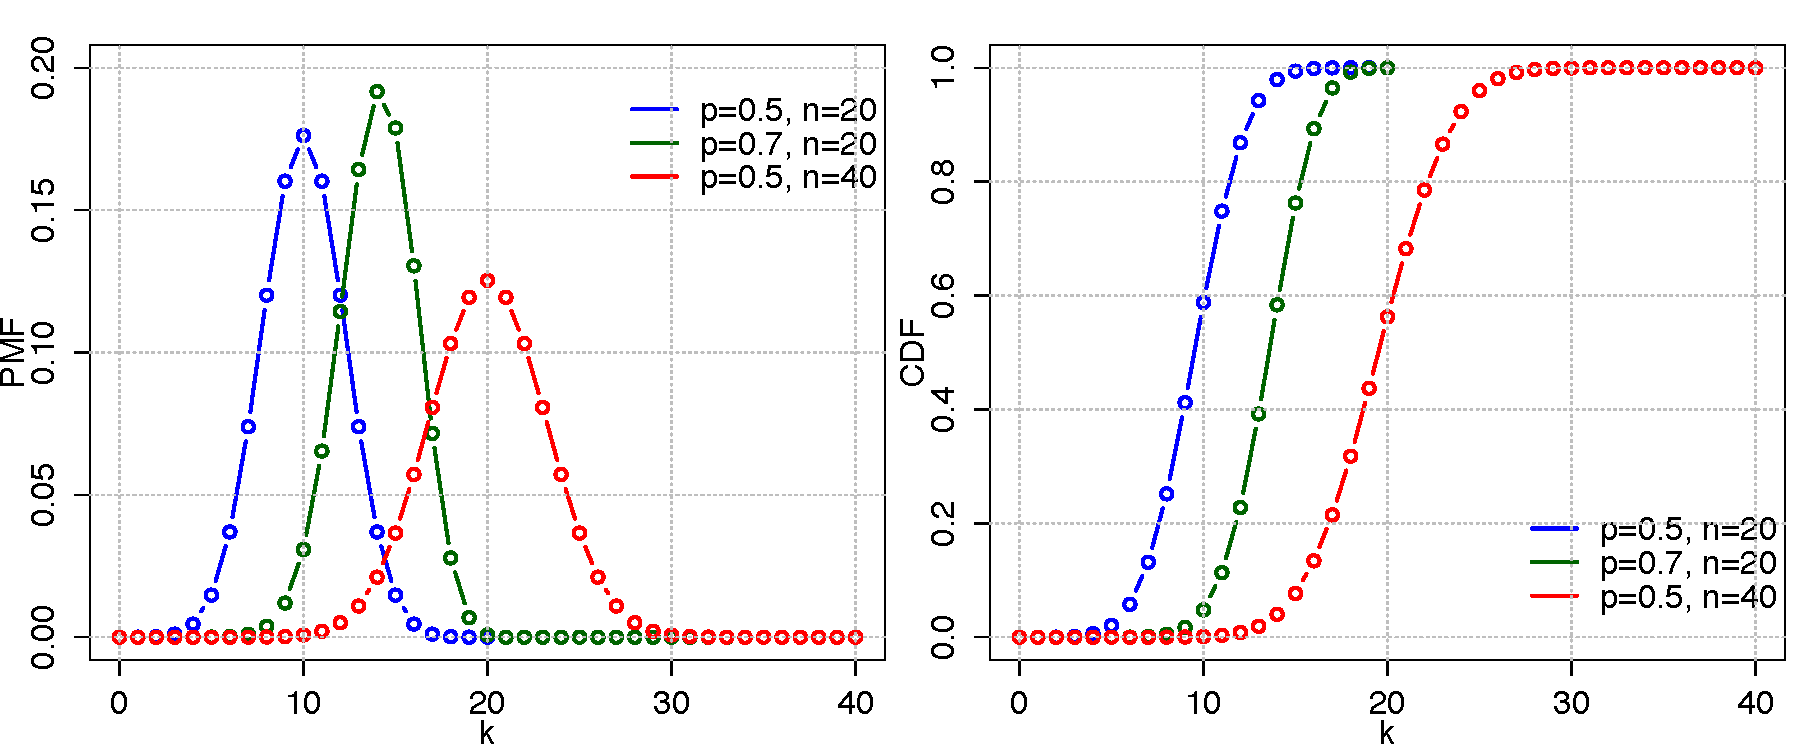
\includegraphics[width=140mm]{pics/Binomial_pmf_cdf.pdf}
% \caption{PMF and CDF of the Binomial distribution plotted using the provided R-code.}
% \label{fig:Bionomial_pmf_cdf}
%\end{figure}
%
%  \bigskip 
%
%\begin{tabular}{p{2cm}cl}
%\textbf{name} & & Binomial (ID: 0000018)\\ 
% 
%\textbf{type} & & discrete \\\textbf{support} & & $k \in \{0,\dots,n\}$
%\end{tabular}
%\subsubsection*{Parameter1}
%
%\noindent\begin{tabular}{p{2cm}cl}
%\textbf{name} & & number of trials \\\textbf{symbol} & & $n$  \\
%\textbf{definition} & & $n \in N, n \ge 0$
%\end{tabular}
%\subsubsection*{Parameter2}
%
%\noindent\begin{tabular}{p{2cm}cl}
%\textbf{name} & & success probability in each trial \\\textbf{symbol} & & $p$  \\
%\textbf{definition} & & $p \in [0,1]$
%\end{tabular}
%\subsubsection*{Functions}
%
%\smallskip \noindent \hspace{.2cm} \textbf{PMF} 
%\begin{equation*}{n \choose k}\, p^k (1-p)^{n-k}\end{equation*}
%
%\smallskip \noindent \hspace{.2cm} \textbf{CDF} 
%\begin{equation*}I_{1-p}(n - k, 1 + k)\end{equation*}
%
%
% \section*{CategoricalNonordered} 
%
%  \bigskip 
%
%\begin{tabular}{p{2cm}cl}
%\textbf{name} & & Categorical Nonordered (ID: 0000038)\\ 
% 
%\textbf{type} & & discrete \\\textbf{support} & & $x \in \{1,\dots,k\}$
%\end{tabular}
%\subsubsection*{Parameter1}
%
%\noindent\begin{tabular}{p{2cm}cl}
%\textbf{name} & & number of categories \\\textbf{symbol} & & $k$  \\
%\textbf{definition} & & $k > 0, k \in Z$
%\end{tabular}
%\subsubsection*{Parameter1}
%
%\noindent\begin{tabular}{p{2cm}cl}
%\textbf{name} & & event probabilities \\\textbf{symbol} & & $p_1, \ldots, p_k$  \\
%\textbf{definition} & & $p_1, \ldots, p_k, \Sigma p_i = 1$
%\end{tabular}
%\subsubsection*{Functions}
%
%\smallskip \noindent \hspace{.2cm} \textbf{PMF} 
%\begin{equation*}p(x=i)=p_i\end{equation*}
%
%\smallskip \noindent \hspace{.2cm} \textbf{CDF} 
%\begin{equation*}undefined\end{equation*}
%\section*{CategoricalOrdered} 
%
%  \bigskip 
%
%\begin{tabular}{p{2cm}cl}
%\textbf{name} & & Categorical Ordered (ID: 0000028)\\ 
% 
%\textbf{type} & & discrete \\\textbf{support} & & $x \in \{1,\dots,k\}$
%\end{tabular}
%\subsubsection*{Parameter1}
%
%\noindent\begin{tabular}{p{2cm}cl}
%\textbf{name} & & number of categories \\\textbf{symbol} & & $k$  \\
%\textbf{definition} & & $k > 0, k \in Z$
%\end{tabular}
%\subsubsection*{Parameter1}
%
%\noindent\begin{tabular}{p{2cm}cl}
%\textbf{name} & & event probabilities \\\textbf{symbol} & & $p_1, \ldots, p_k$  \\
%\textbf{definition} & & $p_1, \ldots, p_k, \Sigma p_i = 1$
%\end{tabular}
%\subsubsection*{Functions}
%
%\smallskip \noindent \hspace{.2cm} \textbf{PMF} 
%\begin{equation*}p(x=i)=p_i\end{equation*}
%
%\smallskip \noindent \hspace{.2cm} \textbf{CDF} 
%\begin{equation*}\begin{cases}
%    0 & \text{for }x<1 \\
%    \sum_{j=1}^i p_j & \text{for }x \in [i,i+1) \\
%    1 & \text{for }x \geq k
%    \end{cases}\end{equation*}
%
%
%\section*{GeneralizedPoisson} 
%
%  \bigskip 
%
%\begin{tabular}{p{2cm}cl}
%\textbf{name} & & Generalized Poisson (ID: 0000177)\\ 
% 
%\textbf{type} & & discrete \\\textbf{support} & & $k \in \{0,1,2,3,\dots\}$
%\end{tabular}
%\subsubsection*{Parameter1}

\noindent\begin{tabular}{p{2cm}cl}
\textbf{name} & & Poisson intensity \\\textbf{symbol} & & $\lambda$  \\
\textbf{definition} & & $\lambda \in R, \lambda > 0$
\end{tabular}
\subsubsection*{Parameter2}

\noindent\begin{tabular}{p{2cm}cl}
\textbf{name} & & dispersion \\\textbf{symbol} & & $\delta$  \\
\textbf{definition} & & $\max(-1,-\lambda/4) < \delta < 1$
\end{tabular}
\subsubsection*{Functions}

\smallskip \noindent \hspace{.2cm} \textbf{PMF} 
\begin{equation*}\frac{\lambda (\lambda+k\delta)^{k-1}\times e^{-\lambda - k \delta}}{k!}\end{equation*}

\smallskip \noindent \hspace{.2cm} \textbf{CDF} 
\begin{equation*}-\end{equation*}

  
  \section*{NegativeBinomial1} 

  \bigskip 

\begin{tabular}{p{2cm}cl}
\textbf{name} & & Negative Binomial 1 (ID: 0000055)\\ 
 
\textbf{type} & & discrete \\\textbf{support} & & $k \in \{0,1,2,3,\dots\}$
\end{tabular}

\begin{figure}[htb!]
\centering
  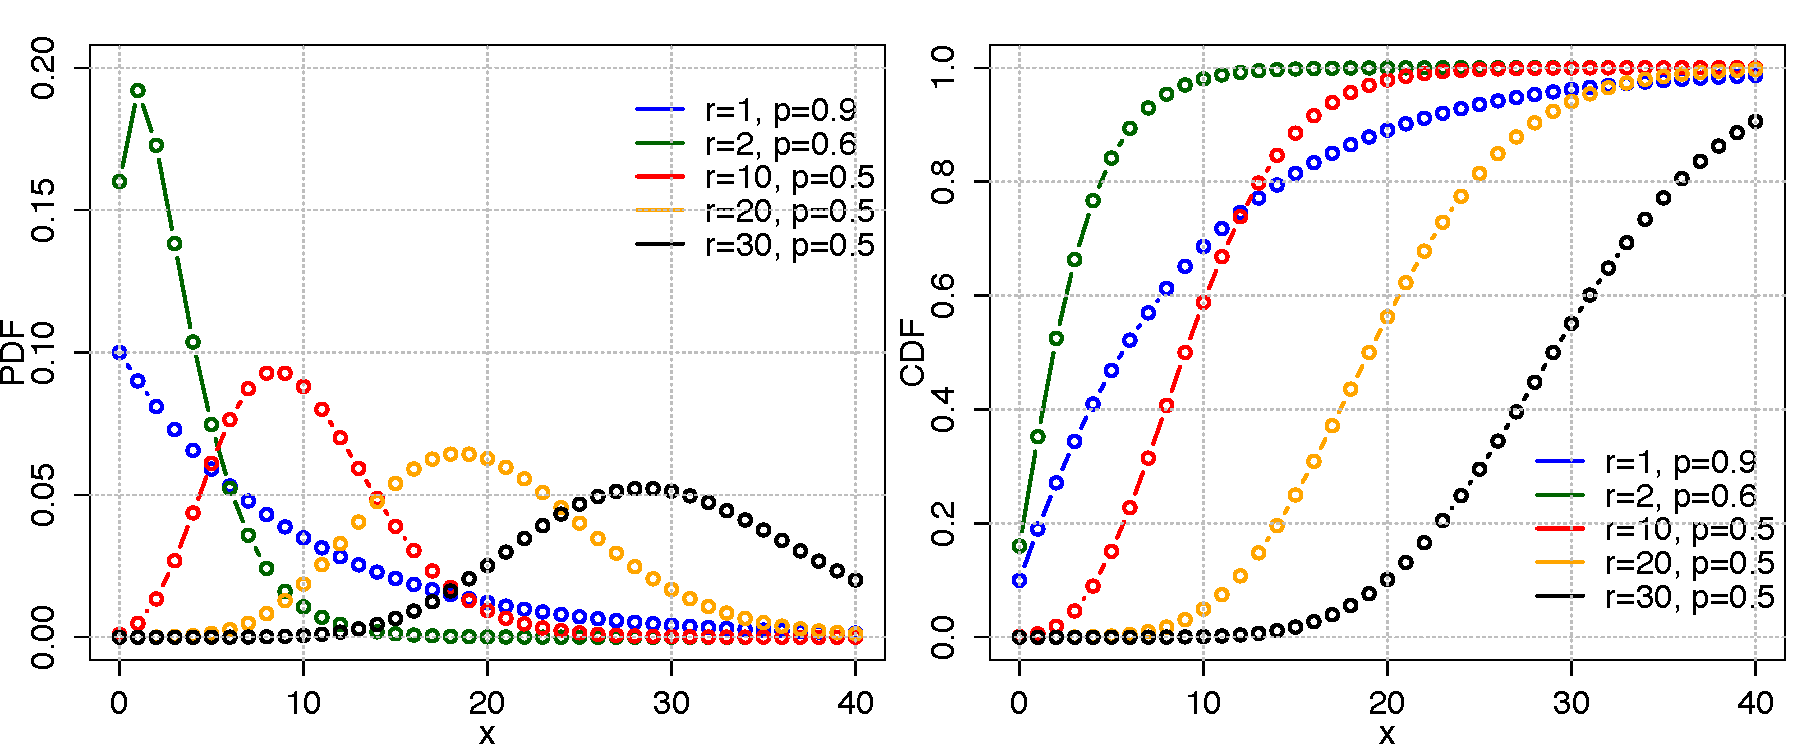
\includegraphics[width=140mm]{pics/NB1_pmf_cdf.pdf}
 \caption{PMF and CDF of the Negative Binomial distribution, NB1,
plotted using the provided R-code.}
 \label{fig:NB1pmfcdf}
\end{figure}

\subsubsection*{Parameter1}

\noindent\begin{tabular}{p{2cm}cl}
\textbf{name} & & number of failures \\\textbf{symbol} & & $r$  \\
\textbf{definition} & & $r > 0, r \in N$
\end{tabular}
\subsubsection*{Parameter2}

\noindent\begin{tabular}{p{2cm}cl}
\textbf{name} & & success probability \\\textbf{symbol} & & $p$  \\
\textbf{definition} & & $p \in [0,1]$
\end{tabular}
\subsubsection*{Functions}

\smallskip \noindent \hspace{.2cm} \textbf{PMF} 
\begin{equation*}\binom {k+r-1}k (1-p)^r p^k\end{equation*}

\smallskip \noindent \hspace{.2cm} \textbf{CDF} 
\begin{equation*}1 - I_{p}(k+1, r)\end{equation*}
\section*{NegativeBinomial2} 

  \bigskip 

\begin{tabular}{p{2cm}cl}
\textbf{name} & & Negative Binomial 2 (ID: 0000064)\\ 
 
\textbf{type} & & discrete \\\textbf{support} & & $k \in \{0,1,2,3,\dots\}$
\end{tabular}

\begin{figure}[htb!]
\centering
  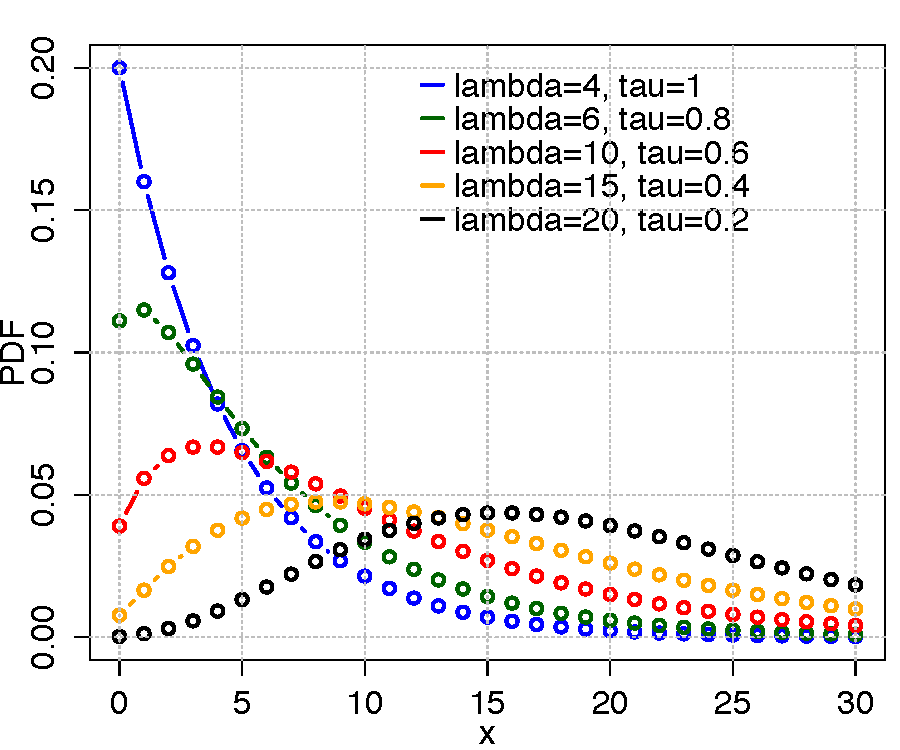
\includegraphics[width=70mm]{pics/NB2_pmf.pdf}
 \caption{PMF of the Negative Binomial distribution, NB2,
 plotted using the provided R-code.}
 \label{fig:NB2pmfcdf}
\end{figure}

\subsubsection*{Parameter1}

\noindent\begin{tabular}{p{2cm}cl}
\textbf{name} & & Poisson intensity \\\textbf{symbol} & & $\lambda$  \\
\textbf{definition} & & $\lambda \in R, \lambda > 0$
\end{tabular}
\subsubsection*{Parameter2}

\noindent\begin{tabular}{p{2cm}cl}
\textbf{name} & & overdispersion \\\textbf{symbol} & & $\tau$  \\
\textbf{definition} & & $\tau \in R$
\end{tabular}
\subsubsection*{Functions}

\smallskip \noindent \hspace{.2cm} \textbf{PMF} 
\begin{equation*}\frac{\Gamma(k + \frac{1}{\tau})}{k!\; \Gamma(\frac{1}{\tau})} \Big(\frac{1}{1+\tau \lambda} \Big)^{\frac{1}{\tau}} 
\Big(\frac{\lambda}{\frac{1}{\tau} + \lambda} \Big)^{k}\end{equation*}

\smallskip \noindent \hspace{.2cm} \textbf{CDF} 
\begin{equation*}-\end{equation*}


\section*{Poisson} 

\begin{figure}[htb!]
\centering
  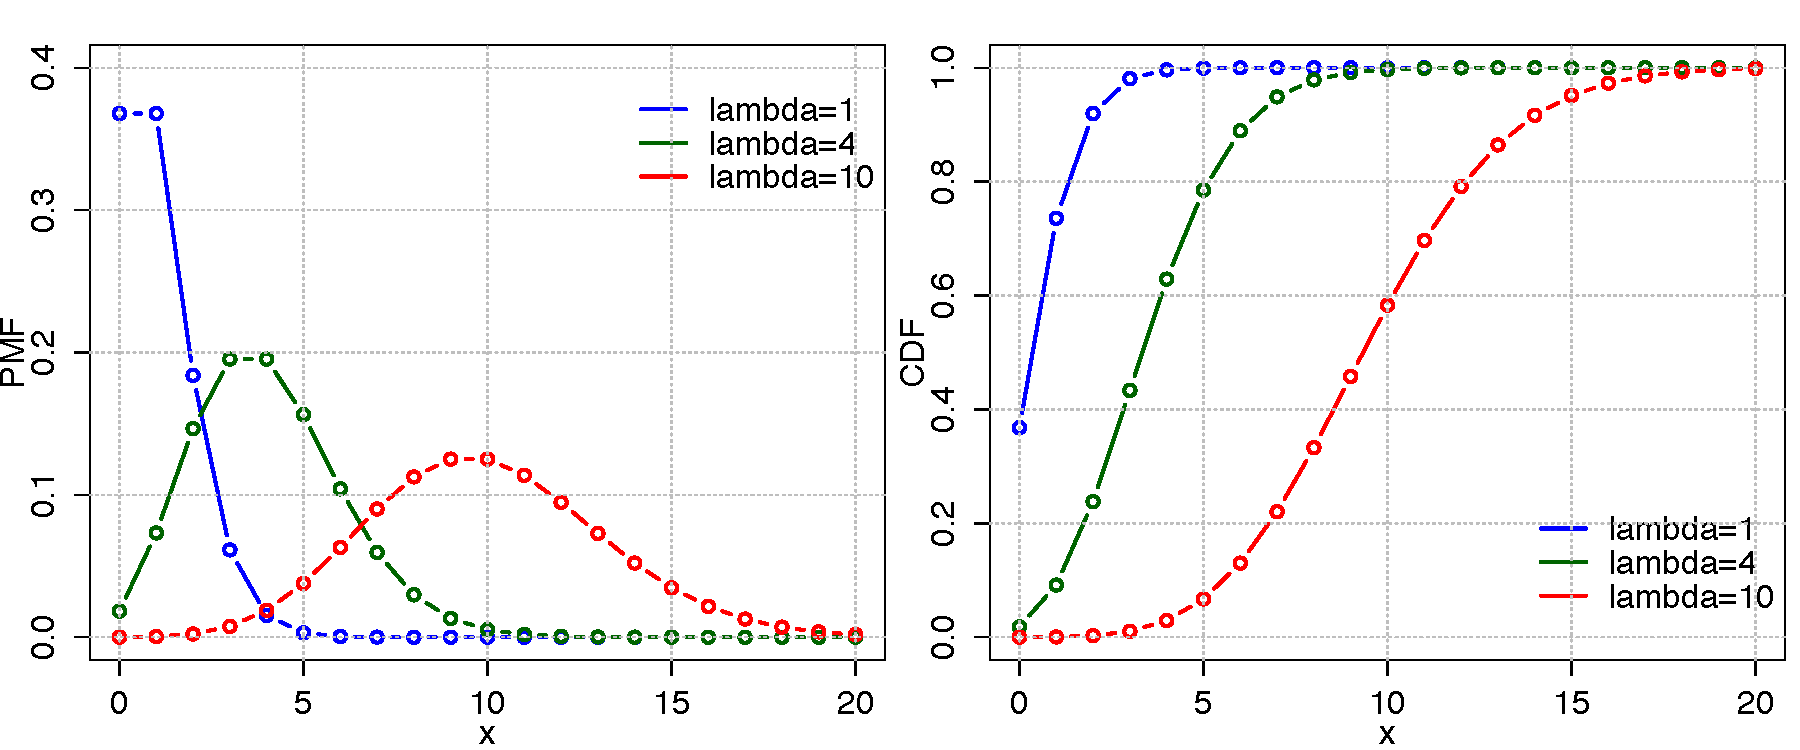
\includegraphics[width=140mm]{pics/Poisson_pmf_cdf.pdf}
 \caption{PMF and CDF of the Poisson distribution plotted using the provided R-code.}
 \label{fig:Poisson_pmf_cdf}
\end{figure}

  \bigskip 

\begin{tabular}{p{2cm}cl}
\textbf{name} & & Poisson (ID: 0000111)\\ 
 
\textbf{type} & & discrete \\\textbf{support} & & $k \in \{0,1,2,3,\dots\}$
\end{tabular}
\subsubsection*{Parameter1}

\noindent\begin{tabular}{p{2cm}cl}
\textbf{name} & & Poisson intensity\\ \textbf{symbol} & & $\lambda$  \\
\textbf{definition} & & $\lambda \in R, \lambda > 0$
\end{tabular}
\subsubsection*{Functions}

\smallskip \noindent \hspace{.2cm} \textbf{PMF} 
\begin{equation*}\frac{\lambda^k}{k!}e^{-\lambda}\end{equation*}

\smallskip \noindent \hspace{.2cm} \textbf{CDF} 
\begin{equation*}\frac{\Gamma(\lfloor k+1 \rfloor,\lambda)}{\lfloor k \rfloor!}\end{equation*}

\paragraph{Note} There are surprising many different names for the Poisson parameter, such as
\label{par:poissonParameterNames}
\begin{itemize}
\item 
\emph{shape} in Distributome, \url{http://www.distributome.org/V3/Distributome.xml.html}
\item 
\emph{mean} or \emph{variance} in Forbes et al. 2010, \cite{Forbes:2010jk}
\item 
\emph{rate} in UncertML, \url{http://www.uncertml.org/distributions/poisson}
\item 
\emph{scale} in Leemis et al. 2008, \url{http://www.math.wm.edu/~leemis/chart/UDR/PDFs/Poisson.pdf}
\end{itemize}
As we have followed the UncertML naming convention, \emph{rate} is the 
code name to be used with ProbOnto.

  
  \section*{ZeroInflatedPoisson} 

  \bigskip 

\begin{tabular}{p{2cm}cl}
\textbf{name} & & Zero-inflated Poisson (ID: 0000210)\\ 
 
\textbf{type} & & discrete \\\textbf{support} & & $k \in \{0,1,2,3,\dots\}$
\end{tabular}

\begin{figure}[htb!]
\centering
  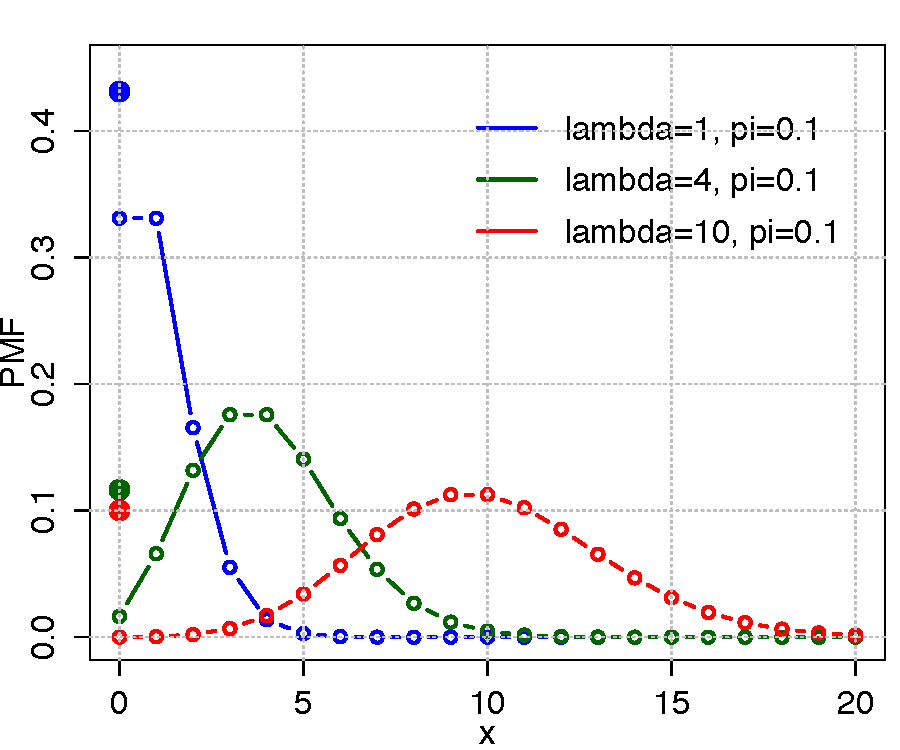
\includegraphics[width=70mm]{pics/ZIP_pmf.pdf}
 \caption{PMF of the ZIP distribution plotted using the provided R-code.}
 \label{fig:Poisson_pmf_cdf}
\end{figure}

\subsubsection*{Parameter1}

\noindent\begin{tabular}{p{2cm}cl}
\textbf{name} & & Poisson intensity \\\textbf{symbol} & & $\lambda$  \\
\textbf{definition} & & $\lambda \in R, \lambda > 0$
\end{tabular}
\subsubsection*{Parameter2}

\noindent\begin{tabular}{p{2cm}cl}
\textbf{name} & & probability of extra zeros \\\textbf{symbol} & & $\pi$  \\
\textbf{definition} & & $0<\pi<1, \pi \in  R$ 
\end{tabular}
\subsubsection*{Functions}

\smallskip \noindent \hspace{.2cm} \textbf{PMF} 
\begin{equation*}\begin{cases}
\pi + (1-\pi) e^{-\lambda}& \text{for } k = 0 \\ 
(1-\pi) e^{-\lambda} \frac{\lambda^k}{k!} & \text{for } k > 0
\end{cases}\end{equation*}

\smallskip \noindent \hspace{.2cm} \textbf{CDF} 
\begin{equation*}-\end{equation*}


%%%%%%%%%%%%%%%%%%%%%%%%%%%%%%%%%%%%%%%%%%%%%%%%%%%%%%%%%%%%%%%%%%%%%
\section{Discrete multivariate distributions}

\section*{Multinomial} 

  \bigskip 

\begin{tabular}{p{2cm}cl}
\textbf{name} & & Multinomial (ID: 0000023)\\ 
 
\textbf{type} & & discrete \\\textbf{support} & & $X_i \in \{0,\dots,n\}, \Sigma X_i = n$
\end{tabular}
\subsubsection*{Parameter1}

\noindent\begin{tabular}{p{2cm}cl}
\textbf{name} & & number of trials \\\textbf{symbol} & & $n$  \\
\textbf{definition} & & $n > 0, n \in N$
\end{tabular}
\subsubsection*{Parameter2}

\noindent\begin{tabular}{p{2cm}cl}
\textbf{name} & & event probabilities \\\textbf{symbol} & & $p_1, \ldots, p_k$  \\
\textbf{definition} & & $p_1, \ldots, p_k, \Sigma p_i = 1$
\end{tabular}
\subsubsection*{Functions}

\smallskip \noindent \hspace{.2cm} \textbf{PMF} 
\begin{equation*}\frac{n!}{x_1!\cdots x_k!} p_1^{x_1} \cdots p_k^{x_k}\end{equation*}

\smallskip \noindent \hspace{.2cm} \textbf{CDF} 
\begin{equation*}-\end{equation*}


%%%%%%%%%%%%%%%%%%%%%%%%%%%%%%%%%%%%%%%%%%%%%%%%%%%%%%%%%%%%%%%%%%%%%
\section{Continuous univariate distributions}

\section*{Beta} 

  \bigskip 

\begin{tabular}{p{2cm}cl}
\textbf{name} & & Beta (ID: 0000009)\\ 
 
\textbf{type} & & continuous \\\textbf{support} & & $x \in (0,1)$
\end{tabular}

\begin{figure}[ht!]
\centering
  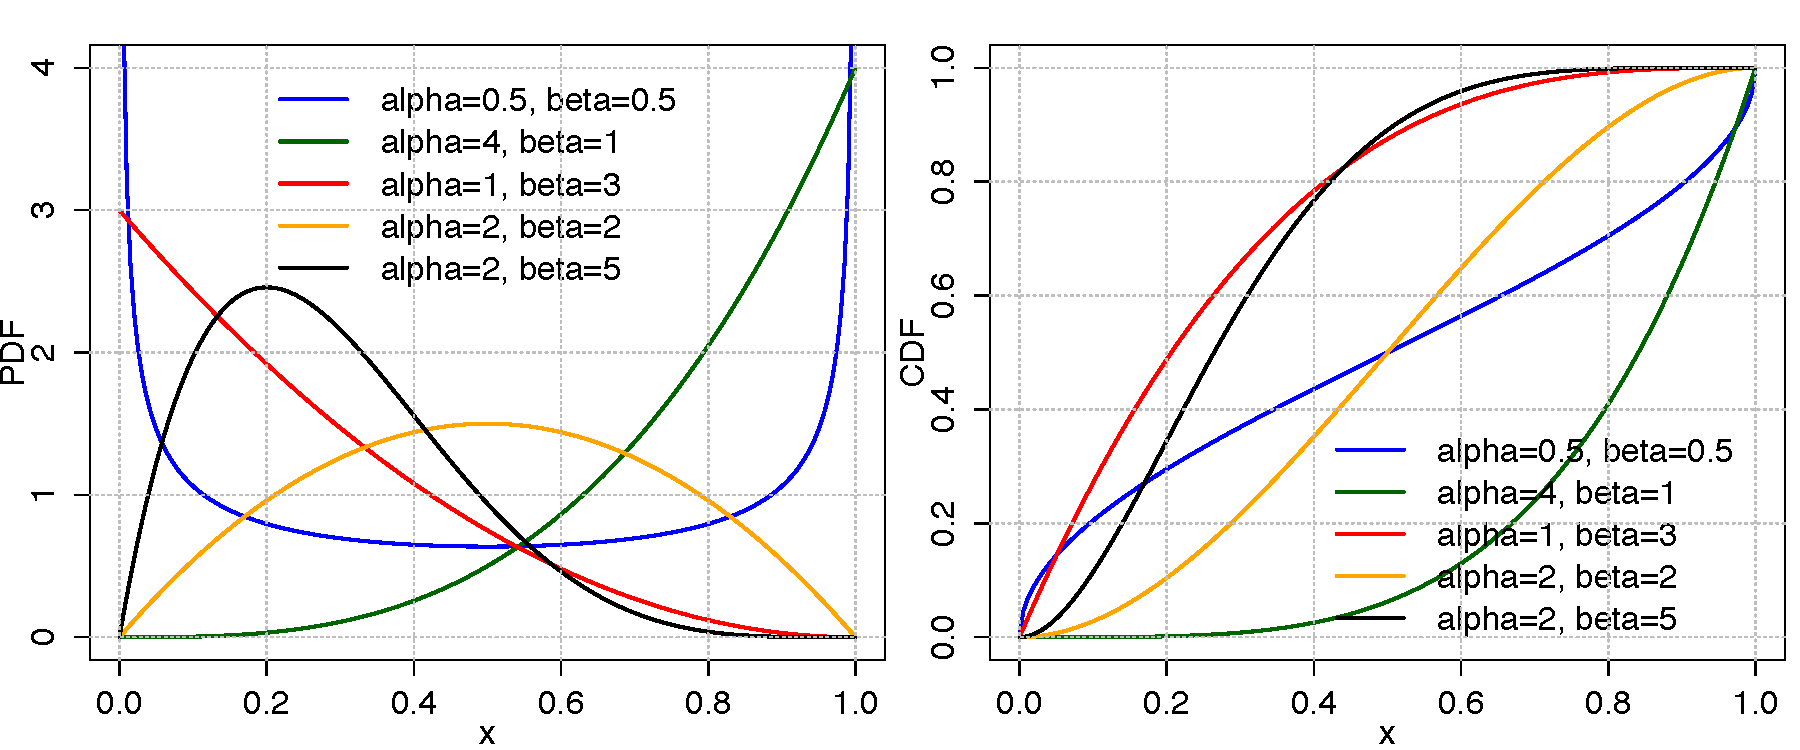
\includegraphics[width=140mm]{pics/Beta_pdf_cdf.pdf}
 \caption{PDF and CDF of the Beta distribution plotted using the provided R-code.}
 \label{fig:Beta_pdf_cdf}
\end{figure}

\subsubsection*{Parameter1}

\noindent\begin{tabular}{p{2cm}cl}
\textbf{name} & & shape \\\textbf{symbol} & & $\alpha$  \\
\textbf{definition} & & $\alpha > 0$
\end{tabular}
\subsubsection*{Parameter2}

\noindent\begin{tabular}{p{2cm}cl}
\textbf{name} & & shape \\\textbf{symbol} & & $\beta$  \\
\textbf{definition} & & $\beta > 0$
\end{tabular}
\subsubsection*{Functions}

\smallskip \noindent \hspace{.2cm} \textbf{PDF} 
\begin{equation*}\frac{x^{\alpha-1}(1-x)^{\beta-1}} {B(\alpha,\beta)} \end{equation*}

\smallskip \noindent \hspace{.2cm} \textbf{CDF} 
\begin{equation*}I_x(\alpha,\beta)\end{equation*}


  \section*{ChiSquared} 

  \bigskip 

\begin{tabular}{p{2cm}cl}
\textbf{name} & & Chi-squared (ID: 0000060)\\ 
 
\textbf{type} & & continuous \\\textbf{support} & & $x \in [0,+\infty)$
\end{tabular}
\subsubsection*{Parameter1}

\noindent\begin{tabular}{p{2cm}cl}
\textbf{name} & & degrees of freedom \\\textbf{symbol} & & $k$  \\
\textbf{definition} & & $k \in N$
\end{tabular}
\subsubsection*{Functions}

\smallskip \noindent \hspace{.2cm} \textbf{PDF} 
\begin{equation*}\frac{1}{2^{\frac{k}{2}}\Gamma\left(\frac{k}{2}\right)}\; x^{\frac{k}{2}-1} e^{-\frac{x}{2}}\end{equation*}

\smallskip \noindent \hspace{.2cm} \textbf{CDF} 
\begin{equation*}\frac{1}{\Gamma\left(\frac{k}{2}\right)}\; \gamma\left(\frac{k}{2},\,\frac{x}{2}\right)\end{equation*}


  \section*{Exponential} 

  \bigskip 

\begin{tabular}{p{2cm}cl}
\textbf{name} & & Exponential (ID: 0000128)\\ 
 
\textbf{type} & & continuous \\\textbf{support} & & $x \in [0,+\infty)$
\end{tabular}
\subsubsection*{Parameter1}

\noindent\begin{tabular}{p{2cm}cl}
\textbf{name} & & rate or inverse scale \\\textbf{symbol} & & $\lambda$  \\
\textbf{definition} & & $\lambda > 0$
\end{tabular}
\subsubsection*{Functions}

\smallskip \noindent \hspace{.2cm} \textbf{PDF} 
\begin{equation*}\lambda e^{-\lambda x}\end{equation*}

\smallskip \noindent \hspace{.2cm} \textbf{CDF} 
\begin{equation*}1 - e^{-\lambda x}\end{equation*}


  \section*{F} 

  \bigskip 

\begin{tabular}{p{2cm}cl}
\textbf{name} & & F (ID: 0000136)\\ 
 
\textbf{type} & & continuous \\\textbf{support} & & $x \in [0,+\infty)$
\end{tabular}

\begin{figure}[ht!]
\centering
  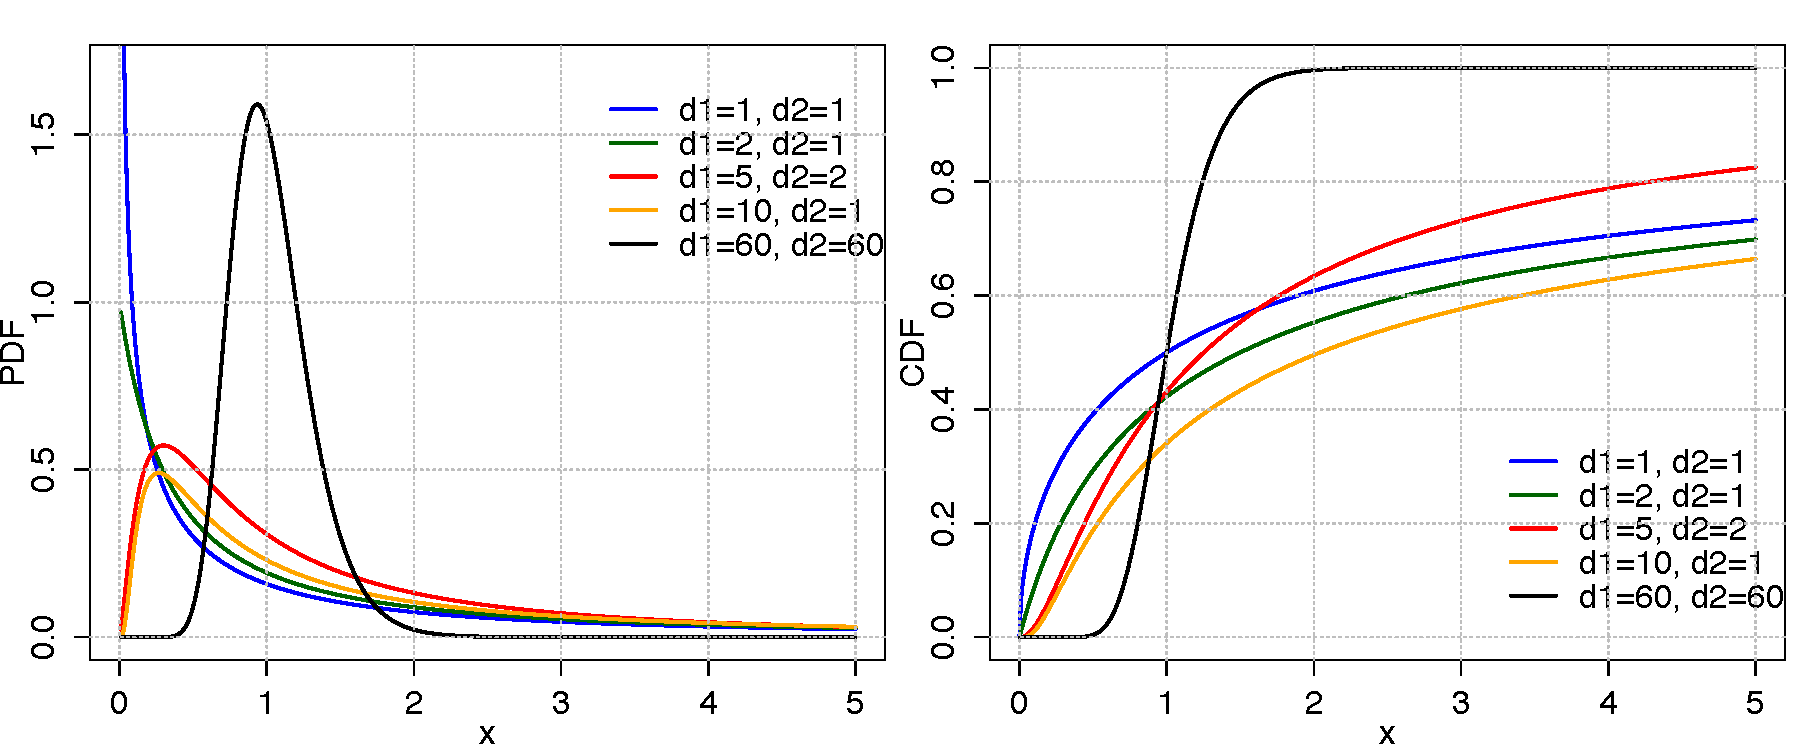
\includegraphics[width=140mm]{pics/F_pdf_cdf.pdf}
 \caption{PDF and CDF of the F distribution plotted using the provided R-code.}
 \label{fig:F_pdf_cdf}
\end{figure}

\subsubsection*{Parameter1}

\noindent\begin{tabular}{p{2cm}cl}
\textbf{name} & & degree of freedom \\\textbf{symbol} & & $d_1$  \\
\textbf{definition} & & $d_1 > 0$
\end{tabular}

\subsubsection*{Parameter2}

\noindent\begin{tabular}{p{2cm}cl}
\textbf{name} & & degree of freedom \\\textbf{symbol} & & $d_2$  \\
\textbf{definition} & & $d_2 > 0$
\end{tabular}
\subsubsection*{Functions}

\smallskip \noindent \hspace{.2cm} \textbf{PDF} 
\begin{equation*}\frac{\sqrt{\frac{(d_1 x)^{d_1}d_2^{d_2}}
{(d_1 x+d_2)^{d_1+d_2}}}}
{x \;B\!\left(\frac{d_1}{2},\frac{d_2}{2}\right)}\end{equation*}

\smallskip \noindent \hspace{.2cm} \textbf{CDF} 
\begin{equation*}I_{\frac{d_1 x}{d_1 x + d_2}} \left(\tfrac{d_1}{2}, \tfrac{d_2}{2} \right)\end{equation*}


  \section*{Gamma} 

  \bigskip 

\begin{tabular}{p{2cm}cl}
\textbf{name} & & Gamma (ID: 0000146)\\ 
 
\textbf{type} & & continuous \\\textbf{support} & & $x \in (0,+\infty)$
\end{tabular}
\subsubsection*{Parameter1}

\noindent\begin{tabular}{p{2cm}cl}
\textbf{name} & & shape \\\textbf{symbol} & & $k$  \\
\textbf{definition} & & $k > 0$
\end{tabular}
\subsubsection*{Parameter2}

\noindent\begin{tabular}{p{2cm}cl}
\textbf{name} & & scale \\\textbf{symbol} & & $\theta$  \\
\textbf{definition} & & $\theta > 0$
\end{tabular}
\subsubsection*{Functions}

\smallskip \noindent \hspace{.2cm} \textbf{PDF} 
\begin{equation*}\frac{1}{\Gamma(k) \theta^k} x^{k \,-\, 1} e^{-\frac{x}{\theta}}\end{equation*}

\smallskip \noindent \hspace{.2cm} \textbf{CDF} 
\begin{equation*}\frac{1}{\Gamma(k)} \gamma\left(k,\, \frac{x}{\theta}\right)\end{equation*}


  \section*{Generalized Gamma \cite{stacy1962generalization}} 
\begin{description} 
\item[Code name] GeneralizedGamma
\item[ID] 0000167
\item[Type] continuous
\item[Support] $x \in (0,+\infty)$
\item[Parameter1]
 \begin{description}
\item[Name] -
\item[symbol] $a$
\item[definition] $a > 0$
\end{description}
\item[Parameter2]
 \begin{description}
\item[Name] -
\item[symbol] $d$
\item[definition] $d > 0$
\end{description}
\item[Parameter3]
 \begin{description}
\item[Name] -
\item[symbol] $p$
\item[definition] $p > 0$
\end{description}
\item[PDF] $\frac{p/a^d}{\Gamma(d/p)} x^{d-1}e^{-(x/a)^p}$
\item[CDF] $\frac{\gamma(d/p, (x/a)^p)}{\Gamma(d/p)}$
  \end{description}


\section*{LogNormal1} 

  \bigskip 

\begin{tabular}{p{2cm}cl}
\textbf{name} & & Log-Normal 1 (ID: 0000230)\\ 
 
\textbf{type} & & continuous \\\textbf{support} & & $x \in (0,+\infty)$
\end{tabular}

\begin{figure}[htb!]
\centering
  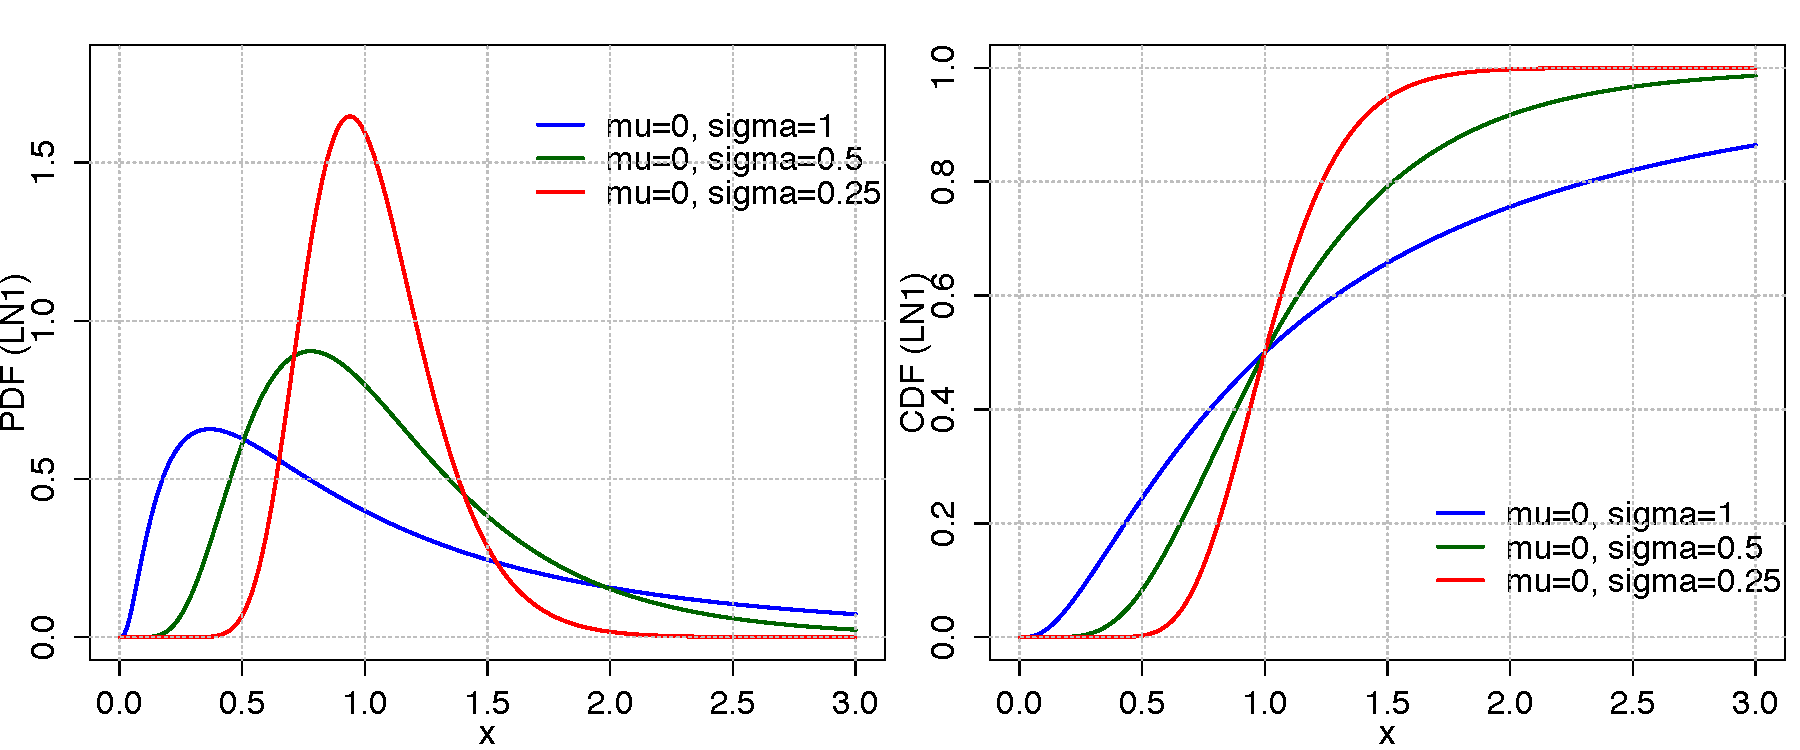
\includegraphics[width=140mm]{pics/LN1_pdf_cdf.pdf}
 \caption{PDF and CDF of the Log-Normal distribution, LN1,
 plotted using the provided R-code.}
 \label{fig:LN1pdfcdf}
\end{figure}

\subsubsection*{Parameter1}

\noindent\begin{tabular}{p{2cm}cl}
\textbf{name} & & mean of log(x) \\\textbf{symbol} & & $\mu$  \\
\textbf{definition} & & $\mu \in R$
\end{tabular}
\subsubsection*{Parameter2}

\noindent\begin{tabular}{p{2cm}cl}
\textbf{name} & & shape \\\textbf{symbol} & & $\sigma$  \\
\textbf{definition} & & $\sigma > 0$
\end{tabular}
\subsubsection*{Functions}

\smallskip \noindent \hspace{.2cm} \textbf{PDF} 
\begin{equation*}\frac{1}{x\sigma\sqrt{2\pi}}\ e^{-\frac{\left(\ln x-\mu\right)^2}{2\sigma^2}}\end{equation*}

\smallskip \noindent \hspace{.2cm} \textbf{CDF} 
\begin{equation*}\frac12 + \frac12\,\text{erf}\Big[\frac{\ln x-\mu}{\sqrt{2}\sigma}\Big]\end{equation*}
\section*{LogNormal2} 

  \bigskip 

\begin{tabular}{p{2cm}cl}
\textbf{name} & & Log-Normal 2 (ID: 0000235)\\ 
 
\textbf{type} & & continuous \\\textbf{support} & & $x \in (0,+\infty)$
\end{tabular}
\subsubsection*{Parameter1}

\noindent\begin{tabular}{p{2cm}cl}
\textbf{name} & & mean of log(x) \\\textbf{symbol} & & $\mu$  \\
\textbf{definition} & & $\mu \in R$
\end{tabular}
\subsubsection*{Parameter2}

\noindent\begin{tabular}{p{2cm}cl}
\textbf{name} & & shape \\\textbf{symbol} & & $v$  \\
\textbf{definition} & & $v > 0$
\end{tabular}
\subsubsection*{Functions}

\smallskip \noindent \hspace{.2cm} \textbf{PDF} 
\begin{equation*}\frac{1}{x\sqrt{v}\sqrt{2\pi}}\ e^{-\frac{\left(\ln x-\mu\right)^2}{2 v}}\end{equation*}

\smallskip \noindent \hspace{.2cm} \textbf{CDF} 
\begin{equation*}-\end{equation*}
\section*{LogNormal3} 

  \bigskip 

\begin{tabular}{p{2cm}cl}
\textbf{name} & & Log-Normal 3 (ID: 0000240)\\ 
 
\textbf{type} & & continuous \\\textbf{support} & & $x \in (0,+\infty)$
\end{tabular}
\subsubsection*{Parameter1}

\noindent\begin{tabular}{p{2cm}cl}
\textbf{name} & & median / geometric mean \\\textbf{symbol} & & $m$  \\
\textbf{definition} & & $m>0$
\end{tabular}
\subsubsection*{Parameter2}

\noindent\begin{tabular}{p{2cm}cl}
\textbf{name} & & shape \\\textbf{symbol} & & $\sigma$  \\
\textbf{definition} & & $\sigma > 0$
\end{tabular}
\subsubsection*{Functions}

\smallskip \noindent \hspace{.2cm} \textbf{PDF} 
\begin{equation*}\frac{1}{x\sigma\sqrt{2\pi}}\ e^{-\frac{\left[\ln (x/m)\right]^2}{2\sigma^2}}\end{equation*}

\smallskip \noindent \hspace{.2cm} \textbf{CDF} 
\begin{equation*}-\end{equation*}
\section*{LogNormal4} 

  \bigskip 

\begin{tabular}{p{2cm}cl}
\textbf{name} & & Log-Normal 4 (ID: 0000245)\\ 
 
\textbf{type} & & continuous \\\textbf{support} & & $x \in (0,+\infty)$
\end{tabular}
\subsubsection*{Parameter1}

\noindent\begin{tabular}{p{2cm}cl}
\textbf{name} & & median / geometric mean \\\textbf{symbol} & & $m$  \\
\textbf{definition} & & $m>0$
\end{tabular}
\subsubsection*{Parameter2}

\noindent\begin{tabular}{p{2cm}cl}
\textbf{name} & & coefficient of variation \\\textbf{symbol} & & $cv$  \\
\textbf{definition} & & $cv>0$
\end{tabular}
\subsubsection*{Functions}

\smallskip \noindent \hspace{.2cm} \textbf{PDF} 
\begin{equation*}\frac{1}{x\sqrt{\ln(cv^2+1)}\sqrt{2\pi}}\ e^{-\frac{\left[\ln (x/m)\right]^2}{2\ln(cv^2+1)}}\end{equation*}

\smallskip \noindent \hspace{.2cm} \textbf{CDF} 
\begin{equation*}-\end{equation*}
\section*{LogNormal5} 

  \bigskip 

\begin{tabular}{p{2cm}cl}
\textbf{name} & & Log-Normal 5 (ID: 0000250)\\ 
 
\textbf{type} & & continuous \\\textbf{support} & & $x \in (0,+\infty)$
\end{tabular}
\subsubsection*{Parameter1}

\noindent\begin{tabular}{p{2cm}cl}
\textbf{name} & & mean of log(x)  \\\textbf{symbol} & & $\mu$  \\
\textbf{definition} & & $\mu \in R$
\end{tabular}
\subsubsection*{Parameter2}

\noindent\begin{tabular}{p{2cm}cl}
\textbf{name} & & precision \\\textbf{symbol} & & $\tau$  \\
\textbf{definition} & & $\tau > 0$
\end{tabular}
\subsubsection*{Functions}

\smallskip \noindent \hspace{.2cm} \textbf{PDF} 
\begin{equation*}\sqrt{\frac{\tau}{2 \pi}} \frac{1}{x}e^{-\frac{\tau}{2}(\log x-\mu)^2}\end{equation*}

\smallskip \noindent \hspace{.2cm} \textbf{CDF} 
\begin{equation*}-\end{equation*}


\section*{Normal1} 

\begin{figure}[htb!]
\centering
  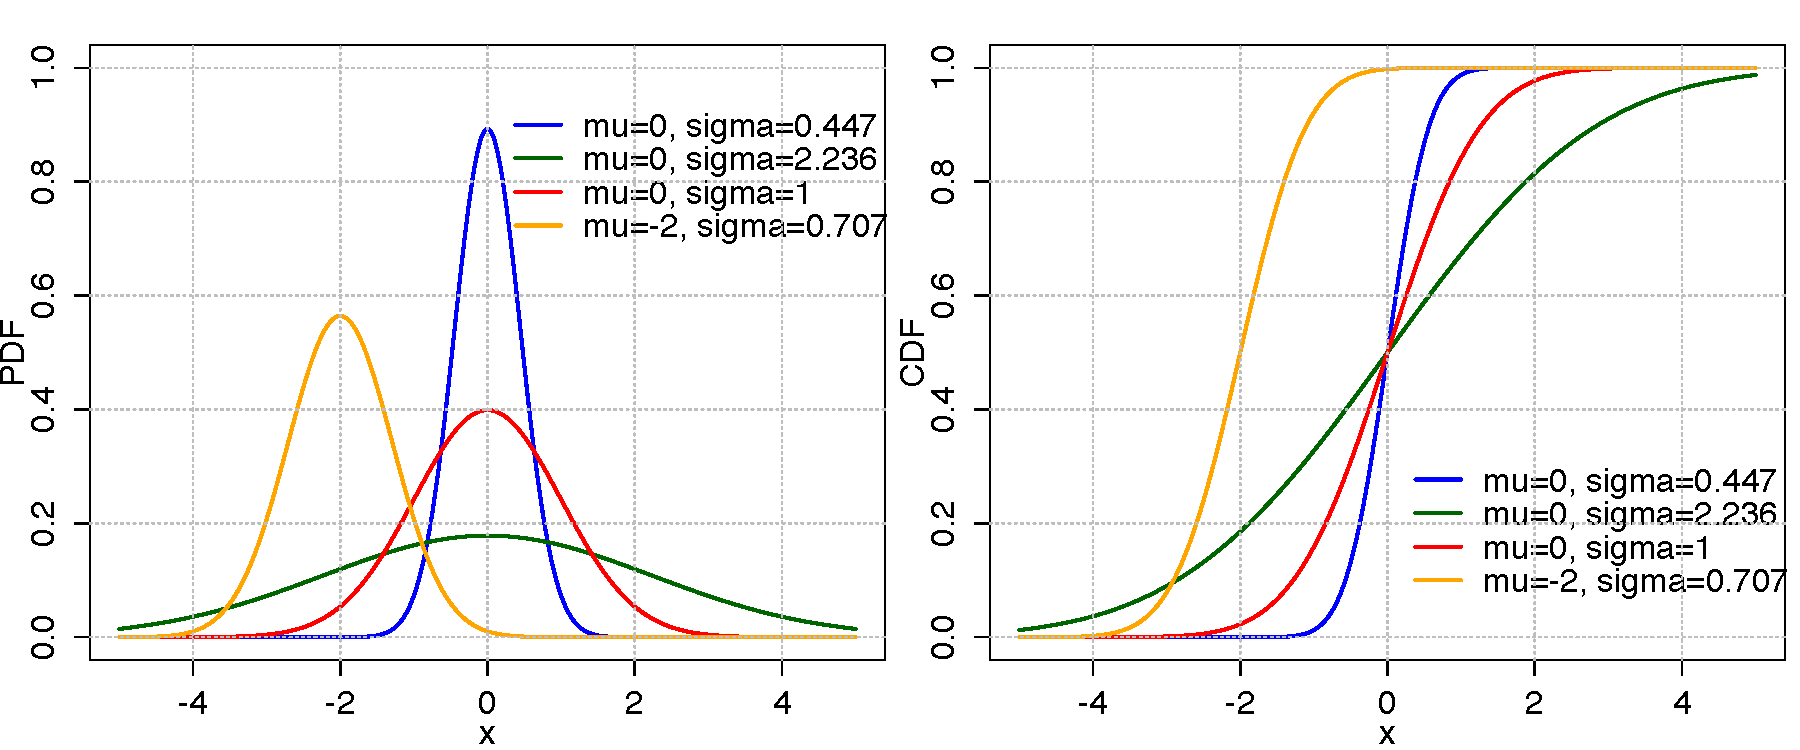
\includegraphics[width=140mm]{pics/Normal1_pdf_cdf.pdf}
 \caption{PDF and CDF of the Normal distribution, N1,
 plotted using the provided R-code.}
 \label{fig:N1pdfcdf}
\end{figure}
  \bigskip 

\begin{tabular}{p{2cm}cl}
\textbf{name} & & Normal 1 (ID: 0000071)\\ 
 
\textbf{type} & & continuous \\\textbf{support} & & $x \in R$
\end{tabular}
\subsubsection*{Parameter1}

\noindent\begin{tabular}{p{2cm}cl}
\textbf{name} & & mean \\\textbf{symbol} & & $\mu$  \\
\textbf{definition} & & $\mu \in  R$
\end{tabular}
\subsubsection*{Parameter2}

\noindent\begin{tabular}{p{2cm}cl}
\textbf{name} & & standard deviation \\\textbf{symbol} & & $\sigma$  \\
\textbf{definition} & & $\sigma> 0$
\end{tabular}
\subsubsection*{Functions}

\smallskip \noindent \hspace{.2cm} \textbf{PDF} 
\begin{equation*}\frac{1}{\sigma \sqrt{2 \pi}}e^{-\frac{(x-\mu)^2}{2\sigma^2}}\end{equation*}

\smallskip \noindent \hspace{.2cm} \textbf{CDF} 
\begin{equation*}\frac12\left[1 + \text{erf}\left( \frac{x-\mu}{\sigma\sqrt{2}}\right)\right]\end{equation*}
\section*{Normal2} 

  \bigskip 

\begin{tabular}{p{2cm}cl}
\textbf{name} & & Normal 2 (ID: 0000081)\\ 
 
\textbf{type} & & continuous \\\textbf{support} & & $x \in R$
\end{tabular}

\begin{figure}[htb!]
\centering
  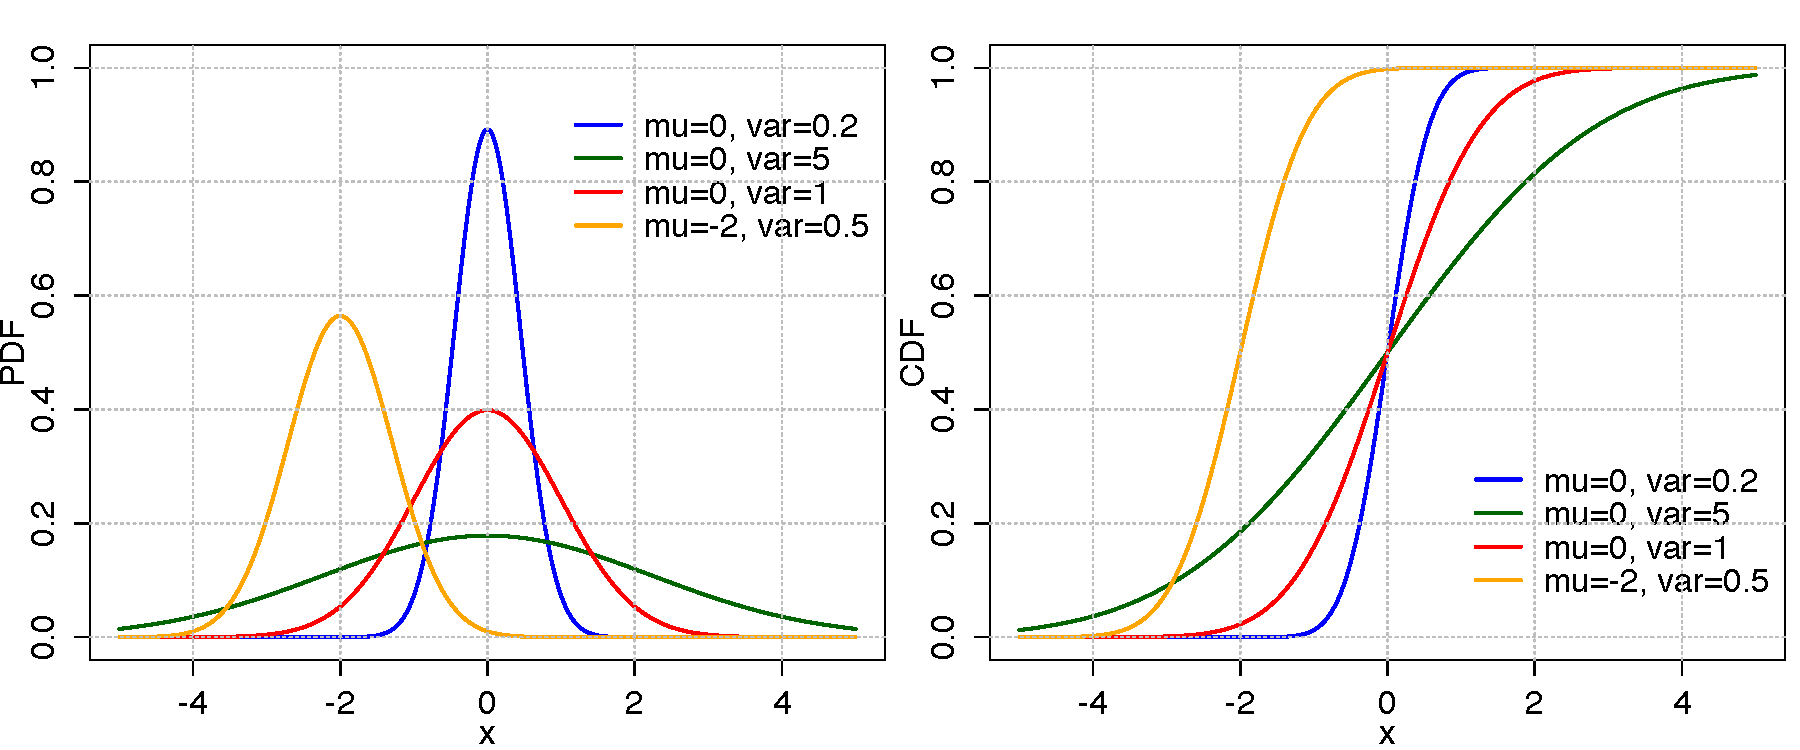
\includegraphics[width=140mm]{pics/Normal2_pdf_cdf.pdf}
 \caption{PDF and CDF of the Normal distribution, N2,
 plotted using the provided R-code.}
 \label{fig:N2pdfcdf}
\end{figure}

\subsubsection*{Parameter1}

\noindent\begin{tabular}{p{2cm}cl}
\textbf{name} & & mean \\\textbf{symbol} & & $\mu$  \\
\textbf{definition} & & $\mu \in  R$
\end{tabular}
\subsubsection*{Parameter2}

\noindent\begin{tabular}{p{2cm}cl}
\textbf{name} & & variance \\\textbf{symbol} & & $v$  \\
\textbf{definition} & & $v>0$
\end{tabular}
\subsubsection*{Functions}

\smallskip \noindent \hspace{.2cm} \textbf{PDF} 
\begin{equation*}\frac{1}{\sqrt{v} \sqrt{2 \pi}}e^{-\frac{(x-\mu)^2}{2*v}}\end{equation*}

\smallskip \noindent \hspace{.2cm} \textbf{CDF} 
\begin{equation*}\frac12\left[1 + \text{erf}\left( \frac{x-\mu}{\sqrt{v}\sqrt{2}}\right)\right]\end{equation*}
\section*{Normal3} 

  \bigskip 

\begin{tabular}{p{2cm}cl}
\textbf{name} & & Normal 3 (ID: 0000088)\\ 
 
\textbf{type} & & continuous \\\textbf{support} & & $x \in R$
\end{tabular}
\subsubsection*{Parameter1}

\noindent\begin{tabular}{p{2cm}cl}
\textbf{name} & & mean \\\textbf{symbol} & & $\mu$  \\
\textbf{definition} & & $\mu \in  R$
\end{tabular}
\subsubsection*{Parameter2}

\noindent\begin{tabular}{p{2cm}cl}
\textbf{name} & & precision \\\textbf{symbol} & & $\tau$  \\
\textbf{definition} & & $\tau>0$
\end{tabular}
\subsubsection*{Functions}

\smallskip \noindent \hspace{.2cm} \textbf{PDF} 
\begin{equation*}\sqrt{\frac{\tau}{2 \pi}} e^{-\frac{\tau}{2}(x-\mu)^2}\end{equation*}
\smallskip \noindent \hspace{.2cm} \textbf{PDF} 
\begin{equation*}\sqrt{\frac{\tau}{2 \pi}} exp\Big(-\frac{\tau}{2}(x-\mu)^2\Big)\end{equation*}

\smallskip \noindent \hspace{.2cm} \textbf{CDF} 
\begin{equation*}-\end{equation*}


\section*{StudentT} 

  \bigskip 

\begin{tabular}{p{2cm}cl}
\textbf{name} & & Student's t-distribution (ID: 0000132)\\ 
 
\textbf{type} & & continuous \\\textbf{support} & & $x \in (-\infty,+\infty)$
\end{tabular}

\begin{figure}[htb!]
\centering
  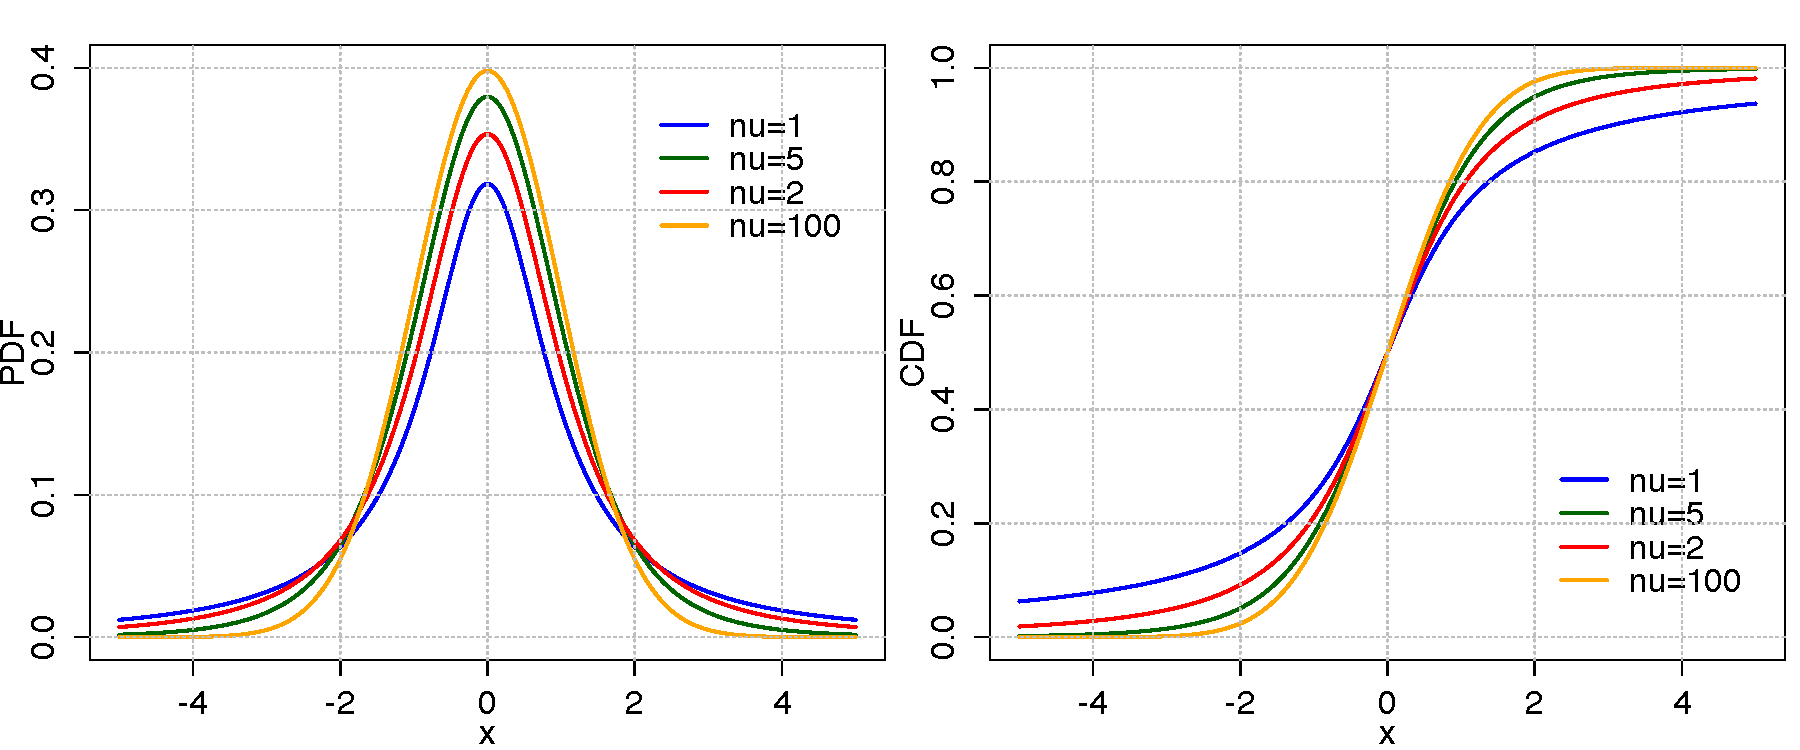
\includegraphics[width=140mm]{pics/StudentT_pdf_cdf.pdf}
 \caption{PDF and CDF of the StudentT distribution plotted using the provided R-code.}
 \label{fig:StudentTpdfcdf}
\end{figure}

\subsubsection*{Parameter1}

\noindent\begin{tabular}{p{2cm}cl}
\textbf{name} & & degrees of freedom \\\textbf{symbol} & & $\nu$  \\
\textbf{definition} & & $\nu > 0, \nu \in  R$
\end{tabular}
\subsubsection*{Functions}

\smallskip \noindent \hspace{.2cm} \textbf{PDF} 
\begin{equation*}\frac{\Gamma \left(\frac{\nu+1}{2} \right)} {\sqrt{\nu\pi}\,\Gamma \left(\frac{\nu}{2} \right)} \left(1+\frac{x^2}{\nu} \right)^{-\frac{\nu+1}{2}}\end{equation*}

\smallskip \noindent \hspace{.2cm} \textbf{CDF} 
\begin{equation*}\begin{matrix}
     \frac{1}{2} + x \Gamma \left( \frac{\nu+1}{2} \right)  \times
     \frac{\,_2F_1 \left ( \frac{1}{2},\frac{\nu+1}{2};\frac{3}{2};
           -\frac{x^2}{\nu} \right)}
     {\sqrt{\pi\nu}\,\Gamma \left(\frac{\nu}{2}\right)}
     \end{matrix}\end{equation*}


\section*{StandardNormal} 

  \bigskip 

\begin{tabular}{p{2cm}cl}
\textbf{name} & & Standard Normal (ID: 0000123)\\ 
 
\textbf{type} & & continuous \\\textbf{support} & & $x \in R$
\end{tabular}

\begin{figure}[htb!]
\centering
  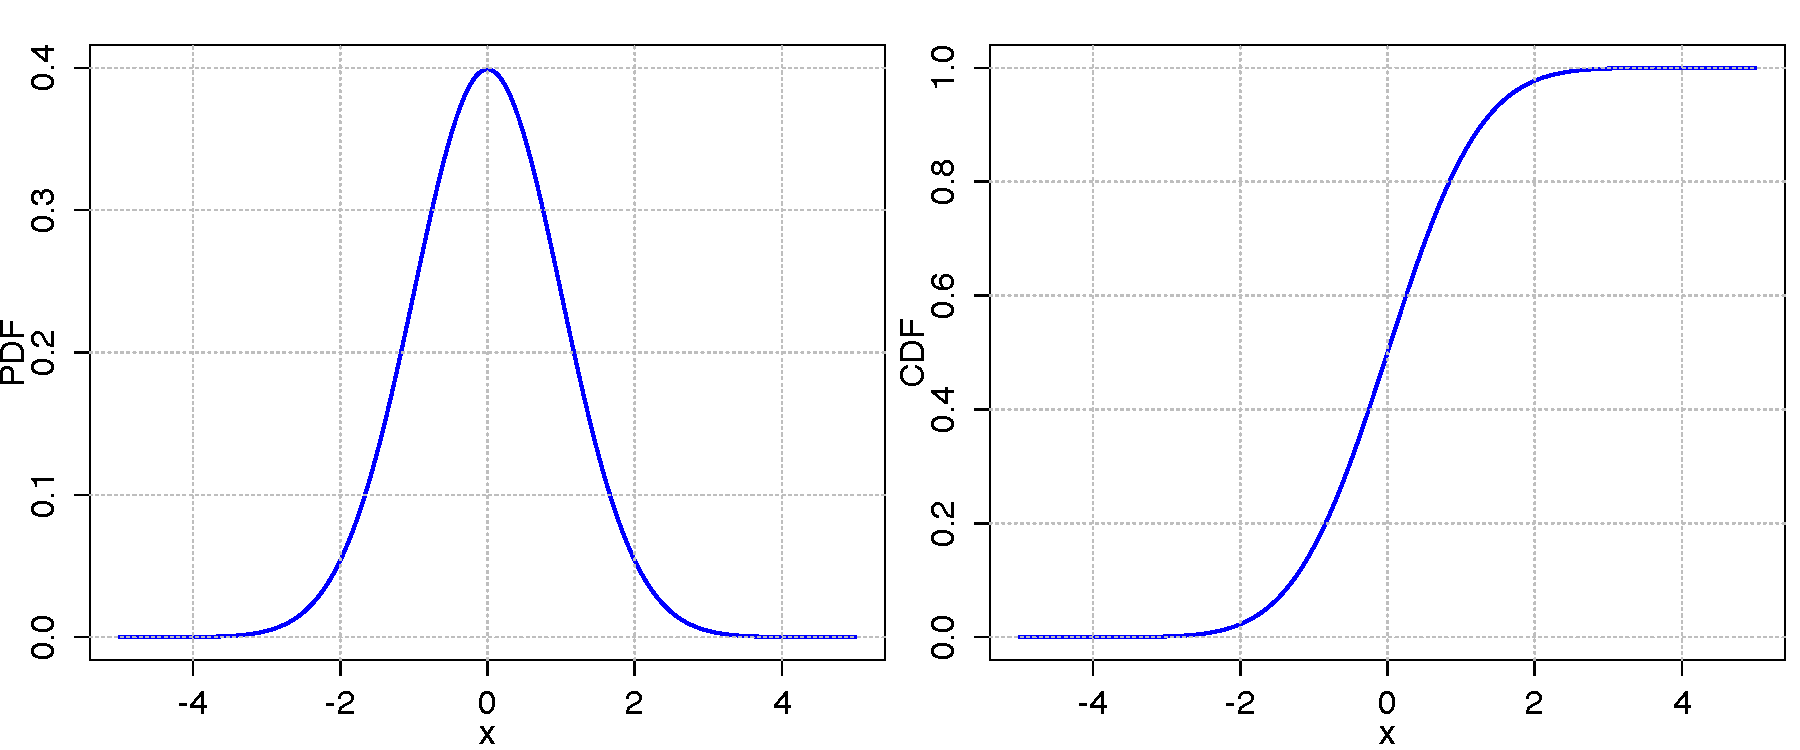
\includegraphics[width=140mm]{pics/StandardNormal_pdf_cdf.pdf}
 \caption{PDF and CDF of the Standard Normal distribution plotted using the provided R-code.}
 \label{fig:StandardNormalpdfcdf}
\end{figure}

\subsubsection*{Parameter1}

\noindent\begin{tabular}{p{2cm}cl}
\textbf{name} & & mean \\\textbf{symbol} & & $\mu$  \\
\textbf{definition} & & $\mu=0$
\end{tabular}
\subsubsection*{Parameter2}

\noindent\begin{tabular}{p{2cm}cl}
\textbf{name} & & standard deviation \\\textbf{symbol} & & $\sigma$  \\
\textbf{definition} & & $\sigma=1$
\end{tabular}
\subsubsection*{Functions}

\smallskip \noindent \hspace{.2cm} \textbf{PDF} 
\begin{equation*}\frac{e^{-\frac{1}{2} x^2}}{\sqrt{2\pi}}\end{equation*}

\smallskip \noindent \hspace{.2cm} \textbf{CDF} 
\begin{equation*}\frac12\left[1 + \text{erf}\left( \frac{x}{\sqrt{2}}\right)\right]\end{equation*}
\section*{StandardUniform} 

  \bigskip 

\begin{tabular}{p{2cm}cl}
\textbf{name} & & Standard Uniform (ID: 0000141)\\ 
 
\textbf{type} & & continuous \\\textbf{support} & & $x \in [0,1]$
\end{tabular}
\subsubsection*{Parameter1}

\noindent\begin{tabular}{p{2cm}cl}
\textbf{name} & & minimum \\
\textbf{symbol} & & $a$  \\
\textbf{definition} & & $a=0$
\end{tabular}
\subsubsection*{Parameter2}

\noindent\begin{tabular}{p{2cm}cl}
\textbf{name} & & maximum \\\textbf{symbol} & & $b$  \\
\textbf{definition} & & $b=1$
\end{tabular}
\subsubsection*{Functions}

\smallskip \noindent \hspace{.2cm} \textbf{PDF} 
\begin{equation*}1\end{equation*}

\smallskip \noindent \hspace{.2cm} \textbf{CDF} 
\begin{equation*}x\end{equation*}


\section*{Uniform} 

  \bigskip 

\begin{tabular}{p{2cm}cl}
\textbf{name} & & Uniform (ID: 0000151)\\ 
 
\textbf{type} & & continuous \\\textbf{support} & & $x \in [a,b]$
\end{tabular}
\subsubsection*{Parameter1}

\noindent\begin{tabular}{p{2cm}cl}
\textbf{name} & & minimum \\\textbf{symbol} & & $a$  \\
\textbf{definition} & & $a \in  R$
\end{tabular}
\subsubsection*{Parameter2}

\noindent\begin{tabular}{p{2cm}cl}
\textbf{name} & & maximum \\\textbf{symbol} & & $b$  \\
\textbf{definition} & & $b \in R, a < b$
\end{tabular}
\subsubsection*{Functions}

\smallskip \noindent \hspace{.2cm} \textbf{PDF} 
\begin{equation*}\begin{cases}
                  \frac{1}{b - a} & \text{for } x \in [a,b]  \\
                  0               & \text{otherwise}
                \end{cases}\end{equation*}

\smallskip \noindent \hspace{.2cm} \textbf{CDF} 
\begin{equation*}\begin{cases}
                  0               & \text{for } x < a \\
                  \frac{x-a}{b-a} & \text{for } x \in [a,b) \\
                  1               & \text{for } x \ge b
                \end{cases}\end{equation*}


  \section*{Weibull1} 

  \bigskip 

\begin{tabular}{p{2cm}cl}
\textbf{name} & & Weibull (ID: 0000182)\\ 
 
\textbf{type} & & continuous \\\textbf{support} & & $x \in [0,+\infty)$
\end{tabular}

\begin{figure}[htb!]
\centering
  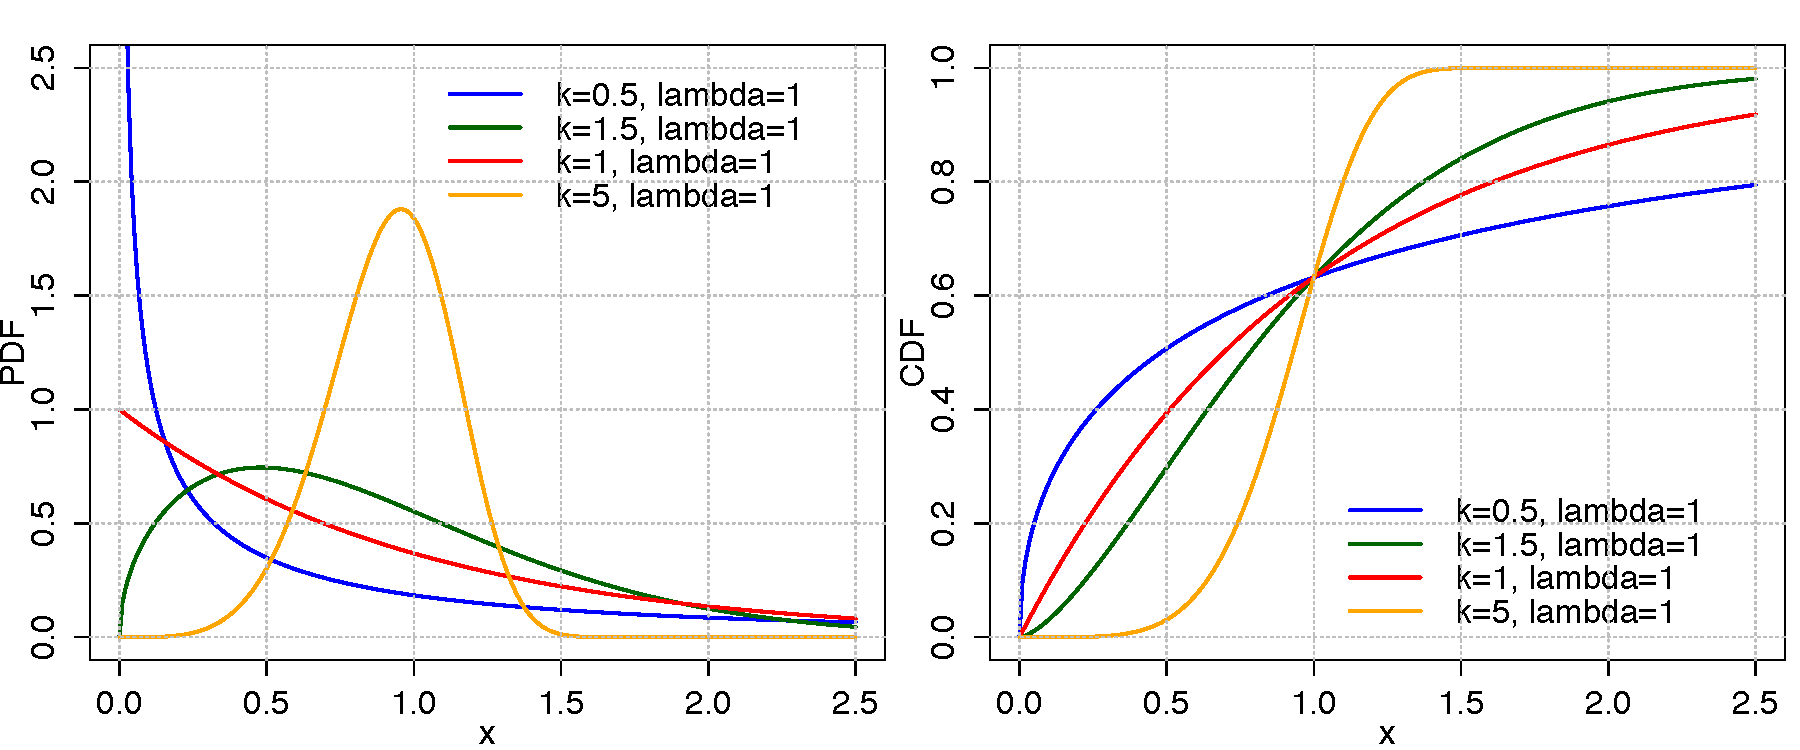
\includegraphics[width=140mm]{pics/Weibull1_pdf_cdf.pdf}
 \caption{PDF and CDF of the Weibull1 distribution plotted using the provided R-code.}
 \label{fig:Weibull1pdfcdf}
\end{figure}


\subsubsection*{Parameter1}

\noindent\begin{tabular}{p{2cm}cl}
\textbf{name} & & scale \\\textbf{symbol} & & $\lambda$  \\
\textbf{definition} & & $\lambda\in (0, +\infty)$
\end{tabular}
\subsubsection*{Parameter2}

\noindent\begin{tabular}{p{2cm}cl}
\textbf{name} & & shape \\\textbf{symbol} & & $k$  \\
\textbf{definition} & & $k\in (0, +\infty)$
\end{tabular}
\subsubsection*{Functions}

\smallskip \noindent \hspace{.2cm} \textbf{PDF} 
\begin{equation*}f(x)=\begin{cases}
\frac{k}{\lambda}\left(\frac{x}{\lambda}\right)^{k-1}e^{-(x/\lambda)^{k}} & x\geq0\\
0 & x<0\end{cases}\end{equation*}

\smallskip \noindent \hspace{.2cm} \textbf{CDF} 
\begin{equation*}\begin{cases}1- e^{-(x/\lambda)^k} & x\geq0\\ 0 & x<0\end{cases}\end{equation*}

   
%%%%%%%%%%%%%%%%%%%%%%%%%%%%%%%%%%%%%%%%%%%%%%%%%%%%%%%%%%%%%%%%%%%%%
\section{Continuous multivariate distributions}


\section*{InverseWishart} 

  \bigskip 

\begin{tabular}{p{2cm}cl}
\textbf{name} & & Inverse-Wishart (ID: 0000215)\\ 
 
\textbf{type} & & continuous \\\textbf{support} & & $X(p \times p) - \text{positive-definite matrix}$
\end{tabular}
\subsubsection*{Parameter1}

\noindent\begin{tabular}{p{2cm}cl}
\textbf{name} & & scale matrix \\\textbf{symbol} & & $\Psi$  \\
\textbf{definition} & & $\Psi > 0, \text{positive-definite matrix}$
\end{tabular}
\subsubsection*{Parameter2}

\noindent\begin{tabular}{p{2cm}cl}
\textbf{name} & & degrees of freedom \\\textbf{symbol} & & $\nu$  \\
\textbf{definition} & & $\nu > p-1, \nu \in  R$
\end{tabular}
\subsubsection*{Functions}

\smallskip \noindent \hspace{.2cm} \textbf{PDF} 
\begin{equation*}\frac{\left|\Psi\right|^{\frac{\nu}{2}}}{2^{\frac{\nu p}{2}}\Gamma_p(\frac{\nu}{2})} \left|X\right|^{-\frac{\nu+p+1}{2}}e^{-\frac{1}{2}\text{tr}(\Psi X^{-1})}\end{equation*}

\smallskip \noindent \hspace{.2cm} \textbf{CDF} 
\begin{equation*}-\end{equation*}


\section*{MultivariateNormal} 

  \bigskip 

\begin{tabular}{p{2cm}cl}
\textbf{name} & & Multivariate Normal (ID: 0000033)\\ 
 
\textbf{type} & & continuous \\\textbf{support} & & $x \in \mu + \text{span}(\Sigma) \subseteq  R^k$
\end{tabular}
\subsubsection*{Parameter1}

\noindent\begin{tabular}{p{2cm}cl}
\textbf{name} & & location \\\textbf{symbol} & & $\mu$  \\
\textbf{definition} & & $\mu \in R^k$
\end{tabular}
\subsubsection*{Parameter2}

\noindent\begin{tabular}{p{2cm}cl}
\textbf{name} & & covariance \\\textbf{symbol} & & $\Sigma$  \\
\textbf{definition} & & $\Sigma \in R^{k\times k}$
\end{tabular}
\subsubsection*{Functions}

\smallskip \noindent \hspace{.2cm} \textbf{PDF} 
\begin{equation*}(2\pi)^{-\frac{k}{2}}|\Sigma|^{-\frac{1}{2}}\, e^{ -\frac{1}{2}(x-\mu)'\Sigma^{-1}(x-\mu) }\end{equation*}

\smallskip \noindent \hspace{.2cm} \textbf{CDF} 
\begin{equation*}\text{no analytic expression}\end{equation*}

  
  \section*{Wishart1} 

  \bigskip 

\begin{tabular}{p{2cm}cl}
\textbf{name} & & Wishart 1 (ID: 0000192)\\ 
 
\textbf{type} & & continuous \\\textbf{support} & & $X(p \times p) - \text{positive definite matrix}$
\end{tabular}
\subsubsection*{Parameter1}

\noindent\begin{tabular}{p{2cm}cl}
\textbf{name} & & scale matrix \\\textbf{symbol} & & $V$  \\
\textbf{definition} & & $V > 0, p\times p - \text{positive definite matrix}$
\end{tabular}
\subsubsection*{Parameter2}

\noindent\begin{tabular}{p{2cm}cl}
\textbf{name} & & degrees of freedom \\\textbf{symbol} & & $n$  \\
\textbf{definition} & & $n > p-1$
\end{tabular}
\subsubsection*{Functions}

\smallskip \noindent \hspace{.2cm} \textbf{PDF} 
\begin{equation*}\frac{|X|^{\frac{n-p-1}{2}} e^{-\frac{\text{tr}(V^{-1}X)}{2}}}{2^\frac{np}{2}|V|^\frac{n}{2}\Gamma_p(\frac{n}{2})}\end{equation*}

\smallskip \noindent \hspace{.2cm} \textbf{CDF} 
\begin{equation*}-\end{equation*}
  
  \section*{Wishart2} 

  \bigskip 

\begin{tabular}{p{2cm}cl}
\textbf{name} & & Wishart 2 (ID: NN)\\ 
 
\textbf{type} & & continuous \\\textbf{support} & & $X(p \times p) - \text{symmetric, positive definite matrix}$
\end{tabular}
\subsubsection*{Parameter1}

\noindent\begin{tabular}{p{2cm}cl}
\textbf{name} & & scale matrix \\\textbf{symbol} & & $R$  \\
\textbf{definition} & & $R(p \times p) - \text{positive definite matrix}$
\end{tabular}
\subsubsection*{Parameter2}

\noindent\begin{tabular}{p{2cm}cl}
\textbf{name} & & $-$ \\
\textbf{symbol} & & $k$  \\
\textbf{definition} & & $-$
\end{tabular}
\subsubsection*{Functions}

\smallskip \noindent \hspace{.2cm} \textbf{PDF} 
\begin{equation*}
|R|^{k/2}|x|^{(k-p-1)/2}e^{-\frac{1}2\,tr(Rx)}\end{equation*}

\smallskip \noindent \hspace{.2cm} \textbf{CDF} 
\begin{equation*}-\end{equation*}

     
%%%%%%%%%%%%%%%%%%%%%%%%%%%%%%%%%%%%%%%%%%%%%%%%%%%%%%%%%%%%%%%%%%%%%
\section{Univariate Mixture Distributions}


\section*{MixtureDistribution} 

  \bigskip 

\begin{tabular}{p{2cm}cl}
\textbf{name} & & Mixture Distribution (ID: 0000014)\\ 
 
\textbf{type} & & continuous/discrete \\
\textbf{support} & & $-$
\end{tabular}

\begin{figure}[htb!]
\centering
  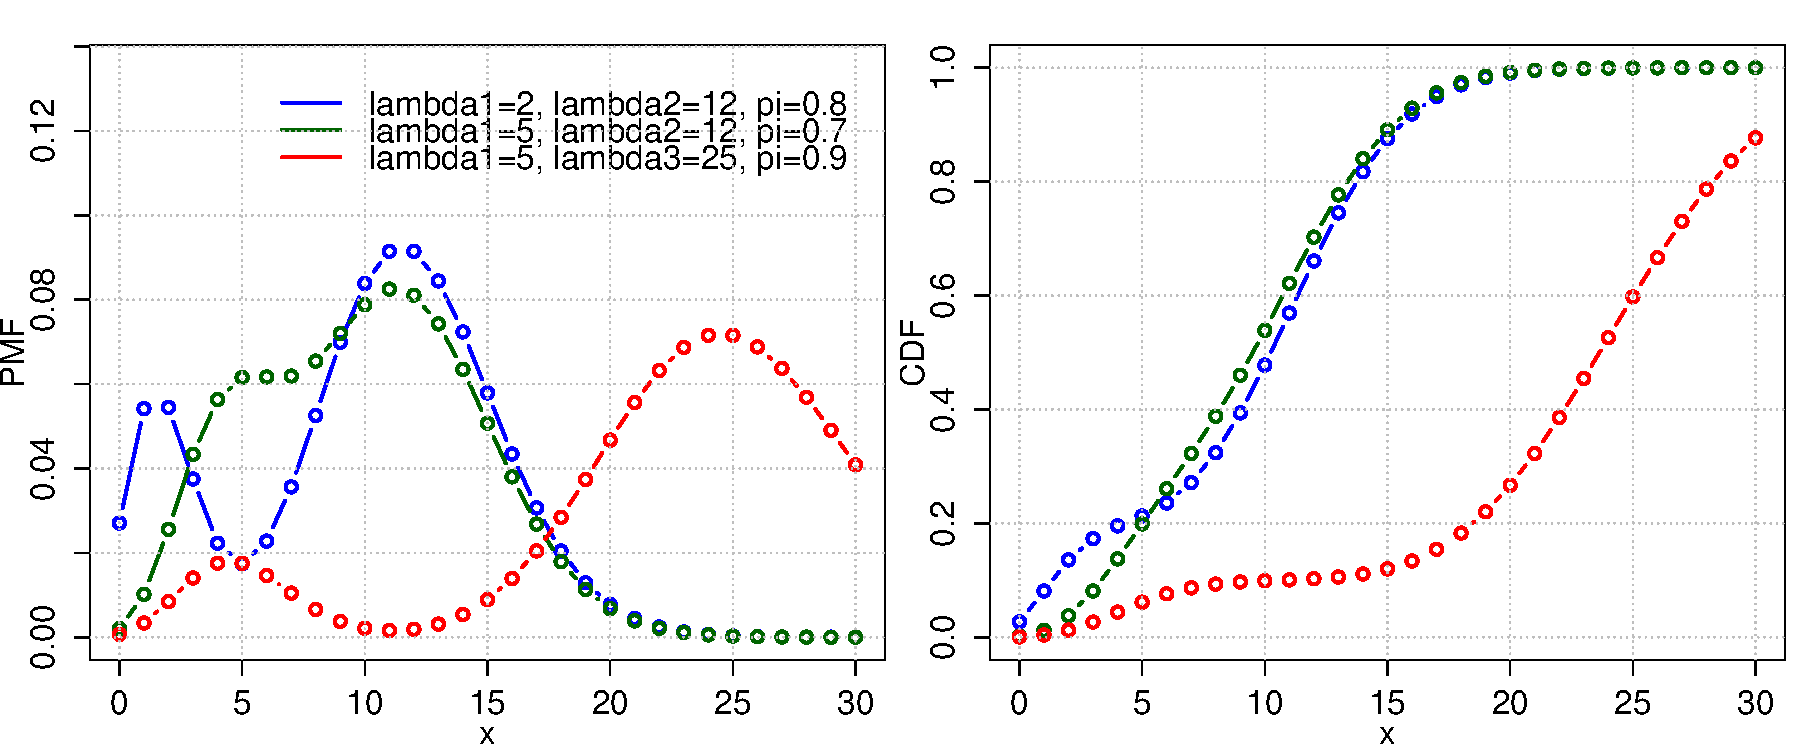
\includegraphics[width=140mm]{pics/MixturePoisson_pmf_cdf}
 \caption{PMF and CDF of the Mixture Poisson distribution plotted using the formula for 
 for various values as shown in the legend of the left plot. The PMF reads: $(1\!-\!\pi) \,\lambda_1^k/k! \,\exp(-\lambda_1) + \pi\,\lambda_2^k / k! \, \exp(-\lambda_2)$. The CDF reads: $(1-\pi)\,\Gamma(\lfloor k+1 , \lambda_1 \rfloor) / \lfloor k \rfloor!+\pi \,\Gamma(\lfloor k+1 , \lambda_2 \rfloor) / \lfloor k \rfloor!$.}
 \label{fig:MixturePoisson_pmf_cdf}
\end{figure}

\subsubsection*{Parameter1}

\noindent\begin{tabular}{p{2cm}cl}
\textbf{name} & & mixing coefficients \\\textbf{symbol} & & $\pi_1, \ldots, \pi_k$  \\
\textbf{definition} & & $\Sigma_{i=1}^K \pi_i=1; 0\le \pi_i \le 1$
\end{tabular}
\subsubsection*{Functions}

\smallskip \noindent \hspace{.2cm} \textbf{PDF} 
\begin{equation*}f(x; \pi, \theta) = \sum_{i=1}^{K} \pi_{i}\; p_i(x; \theta_i)  \end{equation*}
where $p_i(x; \theta_i)$ the PDF of the $i^{th}$ component with parameters $\theta_i$.

\smallskip \noindent \hspace{.2cm} \textbf{PMF} 
\begin{equation*}f(x; \pi, \theta) = \sum_{i=1}^{K} \pi_{i}; p_i(x; \theta_i)  \end{equation*}
where $p_i(x; \theta_i)$ the PMF of the $i^{th}$ component with parameters $\theta_i$.

\smallskip \noindent \hspace{.2cm} \textbf{CDF} 
\begin{equation*}-\end{equation*}




%%%%%%%%%%%%%%%%%%%%%%%%%%%%%%%%%%%%%%%%%%%%%%%%%%%%%%%%%%%%%%%%%%%%%%%%%%%%%%%%%%%%%%%%%%%%%%%%%%%%%%%%%%%%%%%%%%%%%%%%%%%%%%%%%%%%%%%%%%%%%%%%%%%%%%%%%%%%%%%%%%%%%%%%%%%%%%%%%%%%%%%%%%%%%%%%%%%%%%%%%%%%%%%%%%%%%%%%%%%%%%%%%%%%%%%%%%%%%%%%%%%%%%%%%%%%%%%%%%%%%%%%%%%%%%%%%%%%%%%%%%%%%%%%%%%%%%%%%%%%%%%%%%%%%%%%%%%%%%%%%%%
\chapter{New version}

\section*{Bernoulli} 

  \bigskip 

\begin{tabular}{p{2cm}cl}
\textbf{name} & & Bernoulli (ID: 0000000)\\ 
 
\textbf{type} & & discrete \\ 

\textbf{variate} & & $k$, scalar \\ 

\textbf{support} & & $k \in \{0,1\}$
\end{tabular}
\subsubsection*{Parameter: probability}

\noindent\begin{tabular}{p{2cm}cl}
\textbf{name} & & probability \\
\textbf{type} & & scalar \\
\textbf{symbol} & & $p$  \\
\textbf{definition} & & $0<p<1, p \in  R$
\end{tabular}
\subsubsection*{Functions}

\smallskip \noindent \hspace{.2cm} \textbf{PMF} 
\begin{equation*}\begin{cases}
    q=(1-p) & \text{for }k=0 \\ p & \text{for }k=1
    \end{cases}\end{equation*}

\smallskip \noindent \hspace{.2cm} \textbf{PMF in R}  
\begin{equation*}-\end{equation*}

\smallskip \noindent \hspace{.2cm} \textbf{CDF} 
\begin{equation*}\begin{cases}
    0 & \text{for }k<0 \\ q & \text{for }0\leq k<1 \\ 1 & \text{for }k\geq 1
    \end{cases}\end{equation*}

\smallskip \noindent \hspace{.2cm} \textbf{CDF in R} 
\begin{equation*}-\end{equation*}

\smallskip\section*{Beta} 

  \bigskip 

\begin{tabular}{p{2cm}cl}
\textbf{name} & & Beta (ID: 0000009)\\ 
 
\textbf{type} & & continuous \\ 

\textbf{variate} & & $x$, scalar \\ 

\textbf{support} & & $x \in (0,1)$
\end{tabular}
\subsubsection*{Parameter: alpha}

\noindent\begin{tabular}{p{2cm}cl}
\textbf{name} & & shape \\
\textbf{type} & & scalar \\
\textbf{symbol} & & $\alpha$  \\
\textbf{definition} & & $\alpha > 0$
\end{tabular}
\subsubsection*{Parameter: beta}

\noindent\begin{tabular}{p{2cm}cl}
\textbf{name} & & shape \\
\textbf{type} & & scalar \\
\textbf{symbol} & & $\beta$  \\
\textbf{definition} & & $\beta > 0$
\end{tabular}
\subsubsection*{Functions}

\smallskip \noindent \hspace{.2cm} \textbf{PDF} 
\begin{equation*}\frac{x^{\alpha-1}(1-x)^{\beta-1}} {B(\alpha,\beta)} \end{equation*}

\smallskip \noindent \hspace{.2cm} \textbf{PDF in R}  
\begin{equation*}(x^(alpha-1)*(1-x)^(beta-1))/B(alpha,beta)\end{equation*}

\smallskip \noindent \hspace{.2cm} \textbf{CDF} 
\begin{equation*}I_x(\alpha,\beta)\end{equation*}

\smallskip \noindent \hspace{.2cm} \textbf{CDF in R} 
\begin{equation*}Rbeta(x, a, b)\end{equation*}

\smallskip\section*{Binomial} 

  \bigskip 

\begin{tabular}{p{2cm}cl}
\textbf{name} & & Binomial (ID: 0000020)\\ 
 
\textbf{type} & & discrete \\ 

\textbf{variate} & & $k$, scalar \\ 

\textbf{support} & & $k \in \{0,\dots,n\}$
\end{tabular}

\begin{figure}[htb!]
\centering
  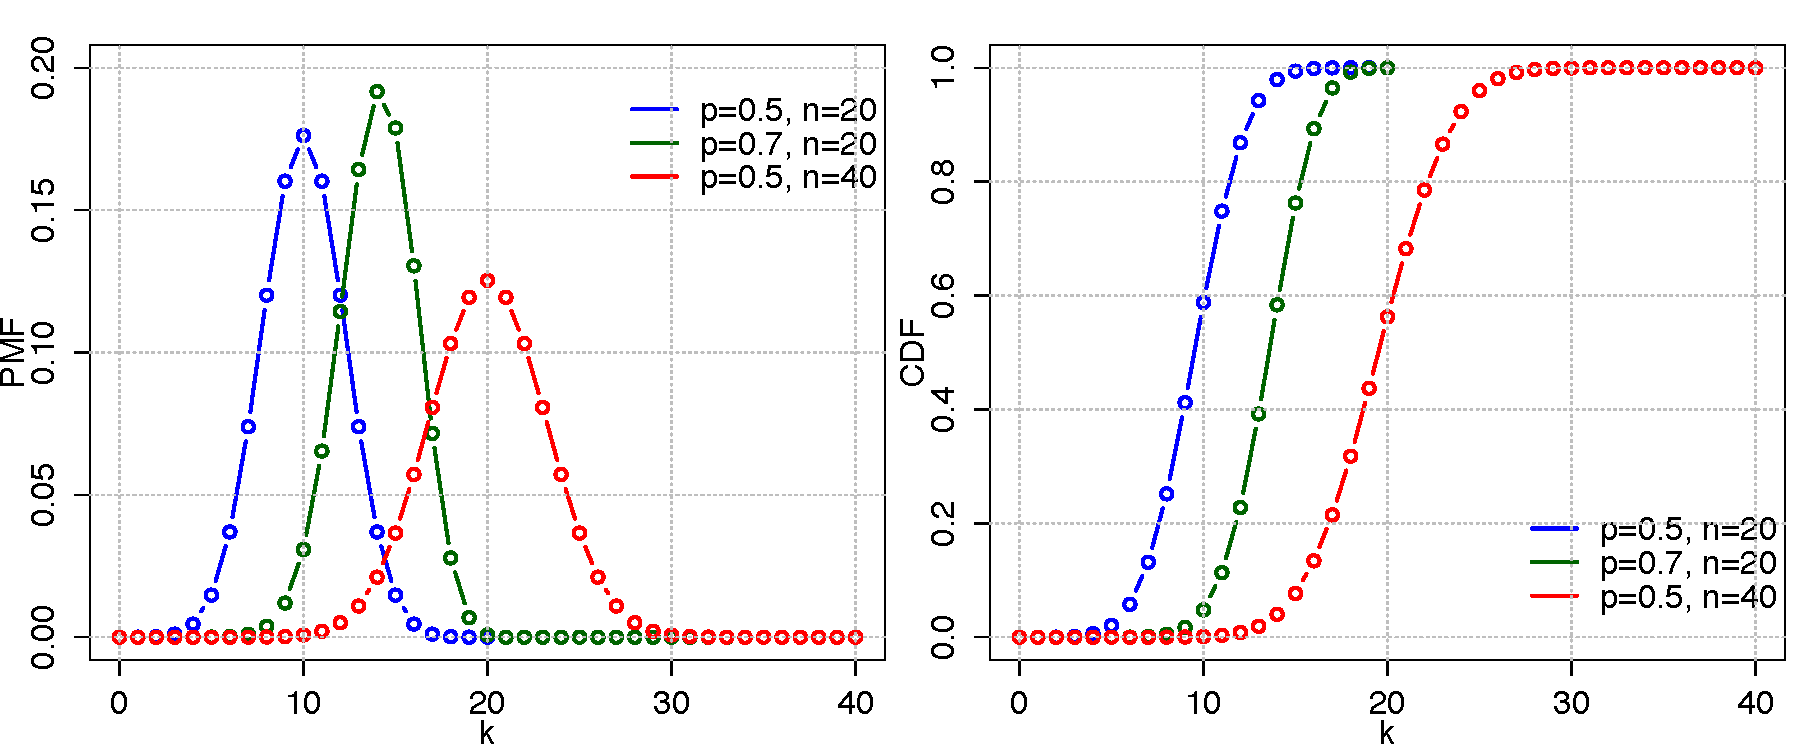
\includegraphics[width=140mm]{pics/Binomial_pmf_cdf.pdf}
 \caption{PMF and CDF of the Binomial distribution plotted using the provided R-code.}
 \label{fig:Bionomial_pmf_cdf}
\end{figure}

\subsubsection*{Parameter: numberOfFailures}

\noindent\begin{tabular}{p{2cm}cl}
\textbf{name} & & number of trials \\
\textbf{type} & & scalar \\
\textbf{symbol} & & $n$  \\
\textbf{definition} & & $n \in N, n \ge 0$
\end{tabular}
\subsubsection*{Parameter: probability}

\noindent\begin{tabular}{p{2cm}cl}
\textbf{name} & & success probability in each trial \\
\textbf{type} & & scalar \\
\textbf{symbol} & & $p$  \\
\textbf{definition} & & $p \in [0,1]$
\end{tabular}
\subsubsection*{Functions}

\smallskip \noindent \hspace{.2cm} \textbf{PMF} 
\begin{equation*}{n \choose k}\, p^k (1-p)^{n-k}\end{equation*}

\smallskip \noindent \hspace{.2cm} \textbf{PMF in R}  
\begin{equation*}choose(n,k) * p^k*(1-p)^(n-k)\end{equation*}

\smallskip \noindent \hspace{.2cm} \textbf{CDF} 
\begin{equation*}I_{1-p}(n - k, 1 + k)\end{equation*}

\smallskip \noindent \hspace{.2cm} \textbf{CDF in R} 
\begin{equation*}Rbeta(1-p, n-k, 1+k)\end{equation*}

\smallskip\section*{CategoricalNonordered} 

  \bigskip 

\begin{tabular}{p{2cm}cl}
\textbf{name} & & Categorical Nonordered (ID: 0000040)\\ 
 
\textbf{type} & & discrete \\ 

\textbf{variate} & & $x$, scalar \\ 

\textbf{support} & & $x \in \{1,\dots,k\}$
\end{tabular}
\subsubsection*{Parameter: categoryProb}

\noindent\begin{tabular}{p{2cm}cl}
\textbf{name} & & category probabilities \\
\textbf{type} & & vector \\
\textbf{symbol} & & $p_1, \ldots, p_k$  \\
\textbf{definition} & & $p_1, \ldots, p_k, \Sigma p_i = 1$
\end{tabular}
\subsubsection*{Functions}

\smallskip \noindent \hspace{.2cm} \textbf{PMF} 
\begin{equation*}p(x=i)=p_i\end{equation*}

\smallskip \noindent \hspace{.2cm} \textbf{PMF in R}  
\begin{equation*}\end{equation*}

\smallskip \noindent \hspace{.2cm} \textbf{CDF} 
\begin{equation*}undefined\end{equation*}

\smallskip \noindent \hspace{.2cm} \textbf{CDF in R} 
\begin{equation*}\end{equation*}

\smallskip\section*{CategoricalOrdered} 

  \bigskip 

\begin{tabular}{p{2cm}cl}
\textbf{name} & & Categorical Ordered (ID: 0000031)\\ 
 
\textbf{type} & & discrete \\ 

\textbf{variate} & & $x$, scalar \\ 

\textbf{support} & & $x \in \{1,\dots,k\}$
\end{tabular}
\subsubsection*{Parameter: categoryProb}

\noindent\begin{tabular}{p{2cm}cl}
\textbf{name} & & category probabilities \\
\textbf{type} & & vector \\
\textbf{symbol} & & $p_1, \ldots, p_k$  \\
\textbf{definition} & & $p_1, \ldots, p_k, \Sigma p_i = 1$
\end{tabular}
\subsubsection*{Functions}

\smallskip \noindent \hspace{.2cm} \textbf{PMF} 
\begin{equation*}p(x=i)=p_i\end{equation*}

\smallskip \noindent \hspace{.2cm} \textbf{PMF in R}  
\begin{equation*}\end{equation*}

\smallskip \noindent \hspace{.2cm} \textbf{CDF} 
\begin{equation*}\begin{cases}
    0 & \text{for }x<1 \\
    \sum_{j=1}^i p_j & \text{for }x \in [i,i+1) \\
    1 & \text{for }x \geq k
    \end{cases}\end{equation*}

\smallskip \noindent \hspace{.2cm} \textbf{CDF in R} 
\begin{equation*}\end{equation*}

\smallskip\section*{Cauchy} 

  \bigskip 

\begin{tabular}{p{2cm}cl}
\textbf{name} & & Cauchy (ID: 0000049)\\ 
 
\textbf{type} & & continuous \\ 

\textbf{variate} & & $x$, scalar \\ 

\textbf{support} & & $x \in (-\infty,+\infty)$
\end{tabular}
\subsubsection*{Parameter: location}

\noindent\begin{tabular}{p{2cm}cl}
\textbf{name} & & location \\
\textbf{type} & & scalar \\
\textbf{symbol} & & $x_0$  \\
\textbf{definition} & & $x_0 \in  R$
\end{tabular}
\subsubsection*{Parameter: scale}

\noindent\begin{tabular}{p{2cm}cl}
\textbf{name} & & scale \\
\textbf{type} & & scalar \\
\textbf{symbol} & & $\gamma$  \\
\textbf{definition} & & $\gamma \in  R$
\end{tabular}
\subsubsection*{Functions}

\smallskip \noindent \hspace{.2cm} \textbf{PDF} 
\begin{equation*}\frac{1}{\pi\gamma\,\left[1 + \left(\frac{x-x_0}{\gamma}\right)^2\right]}\end{equation*}

\smallskip \noindent \hspace{.2cm} \textbf{PDF in R}  
\begin{equation*}\end{equation*}

\smallskip \noindent \hspace{.2cm} \textbf{CDF} 
\begin{equation*}-\end{equation*}

\smallskip \noindent \hspace{.2cm} \textbf{CDF in R} 
\begin{equation*}\end{equation*}

\smallskip\section*{ChiSquared} 

  \bigskip 

\begin{tabular}{p{2cm}cl}
\textbf{name} & & Chi-squared (ID: 0000060)\\ 
 
\textbf{type} & & continuous \\ 

\textbf{variate} & & $x$, scalar \\ 

\textbf{support} & & $x \in [0,+\infty)$
\end{tabular}
\subsubsection*{Parameter: degreesOfFreedom}

\noindent\begin{tabular}{p{2cm}cl}
\textbf{name} & & degrees of freedom \\
\textbf{type} & & scalar \\
\textbf{symbol} & & $k$  \\
\textbf{definition} & & $k \in N$
\end{tabular}
\subsubsection*{Functions}

\smallskip \noindent \hspace{.2cm} \textbf{PDF} 
\begin{equation*}\frac{1}{2^{\frac{k}{2}}\Gamma\left(\frac{k}{2}\right)}\; x^{\frac{k}{2}-1} e^{-\frac{x}{2}}\end{equation*}

\smallskip \noindent \hspace{.2cm} \textbf{PDF in R}  
\begin{equation*}\end{equation*}

\smallskip \noindent \hspace{.2cm} \textbf{CDF} 
\begin{equation*}\frac{1}{\Gamma\left(\frac{k}{2}\right)}\; \gamma\left(\frac{k}{2},\,\frac{x}{2}\right)\end{equation*}

\smallskip \noindent \hspace{.2cm} \textbf{CDF in R} 
\begin{equation*}\end{equation*}

\smallskip\section*{DiracDelta} 

  \bigskip 

\begin{tabular}{p{2cm}cl}
\textbf{name} & & Dirac Delta (ID: 0000069)\\ 
 
\textbf{type} & &  \\ 

\textbf{variate} & & $-$, - \\ 

\textbf{support} & & $-$
\end{tabular}
\subsubsection*{Functions}

\smallskip \noindent \hspace{.2cm} \textbf{} 
\begin{equation*}\end{equation*}

\smallskip \noindent \hspace{.2cm} \textbf{ in R}  
\begin{equation*}\end{equation*}

\smallskip \noindent \hspace{.2cm} \textbf{CDF} 
\begin{equation*}-\end{equation*}

\smallskip \noindent \hspace{.2cm} \textbf{CDF in R} 
\begin{equation*}\end{equation*}

\smallskip\section*{Dirichlet} 

  \bigskip 

\begin{tabular}{p{2cm}cl}
\textbf{name} & & Dirichlet (ID: 0000076)\\ 
 
\textbf{type} & & continuous \\ 

\textbf{variate} & & $x$, vector \\ 

\textbf{support} & & $x_1, \cdots, x_K \quad\text{where}\quad x_i \in [0,1]\quad and \quad\sum_{i=1}^K x_i = 1$
\end{tabular}
\subsubsection*{Parameter: concentration}

\noindent\begin{tabular}{p{2cm}cl}
\textbf{name} & & concentration \\
\textbf{type} & & vector \\
\textbf{symbol} & & $\alpha_1, \cdots, \alpha_K$  \\
\textbf{definition} & & $\alpha_1, \cdots, \alpha_K, \alpha_i > 0$
\end{tabular}
\subsubsection*{Functions}

\smallskip \noindent \hspace{.2cm} \textbf{PDF} 
\begin{equation*}\frac{1}{B(\alpha)} \prod_{i=1}^K x_i^{\alpha_i - 1} \\ \text{where} \quad B(\alpha) = \frac{\prod_{i=1}^K \Gamma(\alpha_i)}{\Gamma\bigl(\sum_{i=1}^K \alpha_i\bigr)} \\ \text{where} \quad \alpha=(\alpha_1,\ldots,\alpha_K)\end{equation*}

\smallskip \noindent \hspace{.2cm} \textbf{PDF in R}  
\begin{equation*}\end{equation*}

\smallskip \noindent \hspace{.2cm} \textbf{CDF} 
\begin{equation*}-\end{equation*}

\smallskip \noindent \hspace{.2cm} \textbf{CDF in R} 
\begin{equation*}\end{equation*}

\smallskip\section*{Exponential} 

  \bigskip 

\begin{tabular}{p{2cm}cl}
\textbf{name} & & Exponential (ID: 0000085)\\ 
 
\textbf{type} & & continuous \\ 

\textbf{variate} & & $x$, scalar \\ 

\textbf{support} & & $x \in [0,+\infty)$
\end{tabular}
\subsubsection*{Parameter: rate}

\noindent\begin{tabular}{p{2cm}cl}
\textbf{name} & & rate or inverse scale \\
\textbf{type} & & scalar \\
\textbf{symbol} & & $\lambda$  \\
\textbf{definition} & & $\lambda > 0$
\end{tabular}
\subsubsection*{Functions}

\smallskip \noindent \hspace{.2cm} \textbf{PDF} 
\begin{equation*}\lambda e^{-\lambda x}\end{equation*}

\smallskip \noindent \hspace{.2cm} \textbf{PDF in R}  
\begin{equation*}\end{equation*}

\smallskip \noindent \hspace{.2cm} \textbf{CDF} 
\begin{equation*}1 - e^{-\lambda x}\end{equation*}

\smallskip \noindent \hspace{.2cm} \textbf{CDF in R} 
\begin{equation*}\end{equation*}

\smallskip\section*{F} 

  \bigskip 

\begin{tabular}{p{2cm}cl}
\textbf{name} & & F (ID: 0000096)\\ 
 
\textbf{type} & & continuous \\ 

\textbf{variate} & & $x$, scalar \\ 

\textbf{support} & & $x \in [0,+\infty)$
\end{tabular}
\subsubsection*{Parameter: numerator}

\noindent\begin{tabular}{p{2cm}cl}
\textbf{name} & & degree of freedom \\
\textbf{type} & & scalar \\
\textbf{symbol} & & $d_1$  \\
\textbf{definition} & & $d_1 > 0$
\end{tabular}
\subsubsection*{Parameter: denominator}

\noindent\begin{tabular}{p{2cm}cl}
\textbf{name} & & degree of freedom \\
\textbf{type} & & scalar \\
\textbf{symbol} & & $d_2$  \\
\textbf{definition} & & $d_2 > 0$
\end{tabular}
\subsubsection*{Functions}

\smallskip \noindent \hspace{.2cm} \textbf{PDF} 
\begin{equation*}\frac{\sqrt{\frac{(d_1 x)^{d_1}d_2^{d_2}}
{(d_1 x+d_2)^{d_1+d_2}}}}
{x B\left(\frac{d_1}{2},\frac{d_2}{2}\right)}\end{equation*}

\smallskip \noindent \hspace{.2cm} \textbf{PDF in R}  
\begin{equation*}\end{equation*}

\smallskip \noindent \hspace{.2cm} \textbf{CDF} 
\begin{equation*}I_{\frac{d_1 x}{d_1 x + d_2}} \left(\tfrac{d_1}{2}, \tfrac{d_2}{2} \right)\end{equation*}

\smallskip \noindent \hspace{.2cm} \textbf{CDF in R} 
\begin{equation*}\end{equation*}

\smallskip\section*{Gamma} 

  \bigskip 

\begin{tabular}{p{2cm}cl}
\textbf{name} & & Gamma (ID: 0000106)\\ 
 
\textbf{type} & & continuous \\ 

\textbf{variate} & & $x$, scalar \\ 

\textbf{support} & & $x \in (0,+\infty)$
\end{tabular}
\subsubsection*{Parameter: shape}

\noindent\begin{tabular}{p{2cm}cl}
\textbf{name} & & shape \\
\textbf{type} & & scalar \\
\textbf{symbol} & & $k$  \\
\textbf{definition} & & $k > 0$
\end{tabular}
\subsubsection*{Parameter: scale}

\noindent\begin{tabular}{p{2cm}cl}
\textbf{name} & & scale \\
\textbf{type} & & scalar \\
\textbf{symbol} & & $\theta$  \\
\textbf{definition} & & $\theta > 0$
\end{tabular}
\subsubsection*{Functions}

\smallskip \noindent \hspace{.2cm} \textbf{PDF} 
\begin{equation*}\frac{1}{\Gamma(k) \theta^k} x^{k \,-\, 1} e^{-\frac{x}{\theta}}\end{equation*}

\smallskip \noindent \hspace{.2cm} \textbf{PDF in R}  
\begin{equation*}\end{equation*}

\smallskip \noindent \hspace{.2cm} \textbf{CDF} 
\begin{equation*}\frac{1}{\Gamma(k)} \gamma\left(k,\, \frac{x}{\theta}\right)\end{equation*}

\smallskip \noindent \hspace{.2cm} \textbf{CDF in R} 
\begin{equation*}\end{equation*}

\smallskip\section*{GeneralizedGamma1} 

  \bigskip 

\begin{tabular}{p{2cm}cl}
\textbf{name} & & Generalized Gamma 1 (ID: 0000123)\\ 
 
\textbf{type} & & continuous \\ 

\textbf{variate} & & $x$, scalar \\ 

\textbf{support} & & $x \in (0,+\infty)$
\end{tabular}
\subsubsection*{Parameter: scale}

\noindent\begin{tabular}{p{2cm}cl}
\textbf{name} & & scale \\
\textbf{type} & & scalar \\
\textbf{symbol} & & $a$  \\
\textbf{definition} & & $a > 0$
\end{tabular}
\subsubsection*{Parameter: shape1}

\noindent\begin{tabular}{p{2cm}cl}
\textbf{name} & & shape \\
\textbf{type} & & scalar \\
\textbf{symbol} & & $d$  \\
\textbf{definition} & & $d > 0$
\end{tabular}
\subsubsection*{Parameter: shape2}

\noindent\begin{tabular}{p{2cm}cl}
\textbf{name} & & shape \\
\textbf{type} & & - \\
\textbf{symbol} & & $p$  \\
\textbf{definition} & & $p > 0$
\end{tabular}
\subsubsection*{Functions}

\smallskip \noindent \hspace{.2cm} \textbf{PDF} 
\begin{equation*}\frac{p/a^d}{\Gamma(d/p)} x^{d-1}e^{-(x/a)^p}\end{equation*}

\smallskip \noindent \hspace{.2cm} \textbf{PDF in R}  
\begin{equation*}\end{equation*}

\smallskip \noindent \hspace{.2cm} \textbf{CDF} 
\begin{equation*}\frac{\gamma(d/p, (x/a)^p)}{\Gamma(d/p)}\end{equation*}

\smallskip \noindent \hspace{.2cm} \textbf{CDF in R} 
\begin{equation*}\end{equation*}

\smallskip\section*{GeneralizedGamma2} 

  \bigskip 

\begin{tabular}{p{2cm}cl}
\textbf{name} & & Generalized Gamma 2 (ID: 0000134)\\ 
 
\textbf{type} & & continuous \\ 

\textbf{variate} & & $x$, scalar \\ 

\textbf{support} & & $0 < a < x$
\end{tabular}
\subsubsection*{Parameter: location}

\noindent\begin{tabular}{p{2cm}cl}
\textbf{name} & & location \\
\textbf{type} & & scalar \\
\textbf{symbol} & & $a$  \\
\textbf{definition} & & $a > 0$
\end{tabular}
\subsubsection*{Parameter: scale}

\noindent\begin{tabular}{p{2cm}cl}
\textbf{name} & & b > 0 \\
\textbf{type} & & scalar \\
\textbf{symbol} & & $b$  \\
\textbf{definition} & & $scale$
\end{tabular}
\subsubsection*{Parameter: shape1}

\noindent\begin{tabular}{p{2cm}cl}
\textbf{name} & & shape \\
\textbf{type} & & scalar \\
\textbf{symbol} & & $c$  \\
\textbf{definition} & & $c > 0$
\end{tabular}
\subsubsection*{Parameter: shape2}

\noindent\begin{tabular}{p{2cm}cl}
\textbf{name} & & shape2 \\
\textbf{type} & & scalar \\
\textbf{symbol} & & $k$  \\
\textbf{definition} & & $k > 0$
\end{tabular}
\subsubsection*{Functions}

\smallskip \noindent \hspace{.2cm} \textbf{PDF} 
\begin{equation*}\frac{k (x-a)^{kc-1}}{b^{kc}\Gamma(c)}\exp\Big[-\Big(\frac{x-a}{b}\Big)^k\Big]\end{equation*}

\smallskip \noindent \hspace{.2cm} \textbf{PDF in R}  
\begin{equation*}\end{equation*}

\smallskip \noindent \hspace{.2cm} \textbf{CDF} 
\begin{equation*}-\end{equation*}

\smallskip \noindent \hspace{.2cm} \textbf{CDF in R} 
\begin{equation*}\end{equation*}

\smallskip\section*{GeneralizedPoisson} 

  \bigskip 

\begin{tabular}{p{2cm}cl}
\textbf{name} & & Generalized Poisson (ID: 0000145)\\ 
 
\textbf{type} & & discrete \\ 

\textbf{variate} & & $k
$, scalar \\ 

\textbf{support} & & $k \in \{0,1,2,3,\dots\}$
\end{tabular}

\begin{figure}[htb!]
\centering
  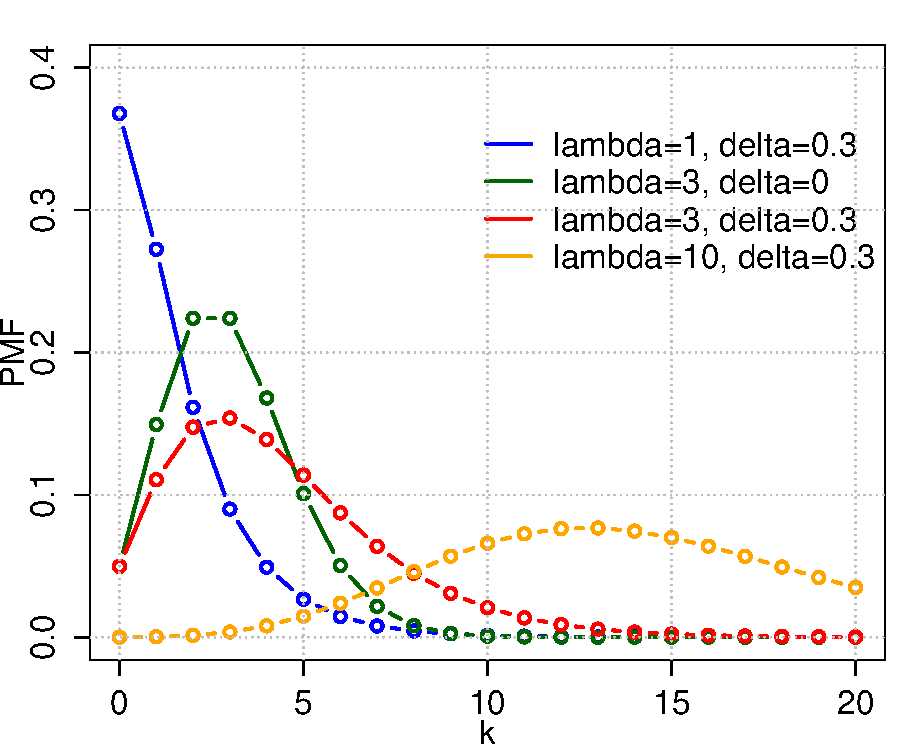
\includegraphics[width=70mm]{pics/GeneralisedPoisson_pmf_cdf}
 \caption{PMF of the Generalised Poisson distribution,
plotted using the provided R-code.}
 \label{fig:NB1pmfcdf}
\end{figure}

\subsubsection*{Parameter: rate}

\noindent\begin{tabular}{p{2cm}cl}
\textbf{name} & & Poisson intensity \\
\textbf{type} & & scalar \\
\textbf{symbol} & & $\lambda$  \\
\textbf{definition} & & $\lambda \in R, \lambda > 0$
\end{tabular}
\subsubsection*{Parameter: dispersion}

\noindent\begin{tabular}{p{2cm}cl}
\textbf{name} & & dispersion \\
\textbf{type} & & scalar \\
\textbf{symbol} & & $\delta$  \\
\textbf{definition} & & $\max(-1,-\lambda/4) < \delta < 1$
\end{tabular}
\subsubsection*{Functions}

\smallskip \noindent \hspace{.2cm} \textbf{PMF} 
\begin{equation*}\frac{\lambda (\lambda+k\delta)^{k-1}\times e^{-\lambda - k \delta}}{k!}\end{equation*}

\smallskip \noindent \hspace{.2cm} \textbf{PMF in R}  
\begin{equation*}\end{equation*}

\smallskip \noindent \hspace{.2cm} \textbf{CDF} 
\begin{equation*}-\end{equation*}

\smallskip \noindent \hspace{.2cm} \textbf{CDF in R} 
\begin{equation*}\end{equation*}

\smallskip\section*{Geometric} 

  \bigskip 

\begin{tabular}{p{2cm}cl}
\textbf{name} & & Geometric (ID: 0000115)\\ 
 
\textbf{type} & & discrete \\ 

\textbf{variate} & & $k
$, scalar \\ 

\textbf{support} & & $k \in \{1,2,3,\dots\}$
\end{tabular}
\subsubsection*{Parameter: probability}

\noindent\begin{tabular}{p{2cm}cl}
\textbf{name} & & success probability \\
\textbf{type} & & scalar \\
\textbf{symbol} & & $p$  \\
\textbf{definition} & & $0< p \leq 1$
\end{tabular}
\subsubsection*{Functions}

\smallskip \noindent \hspace{.2cm} \textbf{PMF} 
\begin{equation*}(1 - p)^{k-1}\,p\end{equation*}

\smallskip \noindent \hspace{.2cm} \textbf{PMF in R}  
\begin{equation*}\end{equation*}

\smallskip \noindent \hspace{.2cm} \textbf{CDF} 
\begin{equation*}1-(1 - p)^k\end{equation*}

\smallskip \noindent \hspace{.2cm} \textbf{CDF in R} 
\begin{equation*}\end{equation*}

\smallskip\section*{Gompertz} 

  \bigskip 

\begin{tabular}{p{2cm}cl}
\textbf{name} & & Gompertz (ID: 0000155)\\ 
 
\textbf{type} & & continuous \\ 

\textbf{variate} & & $x$, scalar \\ 

\textbf{support} & & $x \in (-\infty,+\infty)$
\end{tabular}
\subsubsection*{Parameter: shape}

\noindent\begin{tabular}{p{2cm}cl}
\textbf{name} & & shape \\
\textbf{type} & & scalar \\
\textbf{symbol} & & $\eta$  \\
\textbf{definition} & & $\eta > 0$
\end{tabular}
\subsubsection*{Parameter: scale}

\noindent\begin{tabular}{p{2cm}cl}
\textbf{name} & & scale \\
\textbf{type} & & scalar \\
\textbf{symbol} & & $b$  \\
\textbf{definition} & & $b > 0$
\end{tabular}
\subsubsection*{Functions}

\smallskip \noindent \hspace{.2cm} \textbf{PDF} 
\begin{equation*}b\eta e^{bx}e^{\eta}\exp\left(-\eta e^{bx} \right)\end{equation*}

\smallskip \noindent \hspace{.2cm} \textbf{PDF in R}  
\begin{equation*}\end{equation*}

\smallskip \noindent \hspace{.2cm} \textbf{CDF} 
\begin{equation*}1-\exp\left(-\eta\left(e^{bx}-1 \right)\right)\end{equation*}

\smallskip \noindent \hspace{.2cm} \textbf{CDF in R} 
\begin{equation*}\end{equation*}

\smallskip\section*{Gumbel} 

  \bigskip 

\begin{tabular}{p{2cm}cl}
\textbf{name} & & Gumbel (ID: 0000165)\\ 
 
\textbf{type} & & continuous \\ 

\textbf{variate} & & $x$, scalar \\ 

\textbf{support} & & $x \in (-\infty,+\infty)$
\end{tabular}
\subsubsection*{Parameter: location}

\noindent\begin{tabular}{p{2cm}cl}
\textbf{name} & & location \\
\textbf{type} & & scalar \\
\textbf{symbol} & & $\mu$  \\
\textbf{definition} & & $\mu \in  R$
\end{tabular}
\subsubsection*{Parameter: scale}

\noindent\begin{tabular}{p{2cm}cl}
\textbf{name} & & scale \\
\textbf{type} & & scalar \\
\textbf{symbol} & & $\beta$  \\
\textbf{definition} & & $\beta>0, \beta \in  R$
\end{tabular}
\subsubsection*{Functions}

\smallskip \noindent \hspace{.2cm} \textbf{PDF} 
\begin{equation*}\frac{e^{-e^{-\frac{x-\mu}{\beta}}} e^{-\frac{x-\mu}{\beta}}}{\beta}\end{equation*}

\smallskip \noindent \hspace{.2cm} \textbf{PDF in R}  
\begin{equation*}\end{equation*}

\smallskip \noindent \hspace{.2cm} \textbf{CDF} 
\begin{equation*}e^{-e^{-(x-\mu)/\beta}}\end{equation*}

\smallskip \noindent \hspace{.2cm} \textbf{CDF in R} 
\begin{equation*}\end{equation*}

\smallskip\section*{Hypergeometric} 

  \bigskip 

\begin{tabular}{p{2cm}cl}
\textbf{name} & & Hypergeometric (ID: 0000176)\\ 
 
\textbf{type} & & discrete \\ 

\textbf{variate} & & $k
$, scalar \\ 

\textbf{support} & & $k\, \in\, \left\{\max{(0,\, n+K-N)},\, \dots,\, \min{(n,\, K )}\right\}$
\end{tabular}
\subsubsection*{Parameter: populationSize}

\noindent\begin{tabular}{p{2cm}cl}
\textbf{name} & & population size \\
\textbf{type} & & scalar \\
\textbf{symbol} & & $N$  \\
\textbf{definition} & & $N \in \left\{0,1,2,\dots\right\}$
\end{tabular}
\subsubsection*{Parameter: numberOfTrials}

\noindent\begin{tabular}{p{2cm}cl}
\textbf{name} & & number of trials \\
\textbf{type} & & scalar \\
\textbf{symbol} & & $K$  \\
\textbf{definition} & & $K \in \left\{0,1,2,\dots,N\right\} $
\end{tabular}
\subsubsection*{Parameter: numberOfSuccesses}

\noindent\begin{tabular}{p{2cm}cl}
\textbf{name} & & number of successes \\
\textbf{type} & & scalar \\
\textbf{symbol} & & $n$  \\
\textbf{definition} & & $n \in \left\{0,1,2,\dots,N\right\}$
\end{tabular}
\subsubsection*{Functions}

\smallskip \noindent \hspace{.2cm} \textbf{PMF} 
\begin{equation*}{{{K \choose k} {{N-K} \choose {n-k}}}\over {N \choose n}}\end{equation*}

\smallskip \noindent \hspace{.2cm} \textbf{PMF in R}  
\begin{equation*}\end{equation*}

\smallskip \noindent \hspace{.2cm} \textbf{CDF} 
\begin{equation*}1-{{{n \choose {k+1}}{{N-n} \choose {K-k-1}}}\over {N \choose K}} \,_3F_2\!\!\left[\begin{array}{c}1,\ k+1-K,\ k+1-n \\ k+2,\ N+k+2-K-n\end{array};1\right]\end{equation*}

\smallskip \noindent \hspace{.2cm} \textbf{CDF in R} 
\begin{equation*}\end{equation*}

\smallskip\section*{InverseGamma} 

  \bigskip 

\begin{tabular}{p{2cm}cl}
\textbf{name} & & Inverse-Gamma (ID: 0000187)\\ 
 
\textbf{type} & & continuous \\ 

\textbf{variate} & & $x$, scalar \\ 

\textbf{support} & & $x \in (0,+\infty)$
\end{tabular}
\subsubsection*{Parameter: shape}

\noindent\begin{tabular}{p{2cm}cl}
\textbf{name} & & shape \\
\textbf{type} & & scalar \\
\textbf{symbol} & & $\alpha$  \\
\textbf{definition} & & $\alpha>0, \alpha \in  R$
\end{tabular}
\subsubsection*{Parameter: scale}

\noindent\begin{tabular}{p{2cm}cl}
\textbf{name} & & scale \\
\textbf{type} & & scalar \\
\textbf{symbol} & & $\beta$  \\
\textbf{definition} & & $\beta>0, \beta \in  R$
\end{tabular}
\subsubsection*{Functions}

\smallskip \noindent \hspace{.2cm} \textbf{PDF} 
\begin{equation*}\frac{\beta^\alpha}{\Gamma(\alpha)} x^{-\alpha - 1} \exp \left(\frac{-\beta}{x}\right)\end{equation*}

\smallskip \noindent \hspace{.2cm} \textbf{PDF in R}  
\begin{equation*}\end{equation*}

\smallskip \noindent \hspace{.2cm} \textbf{CDF} 
\begin{equation*}\frac{\Gamma(\alpha, \beta/x)}{\Gamma(\alpha)}\end{equation*}

\smallskip \noindent \hspace{.2cm} \textbf{CDF in R} 
\begin{equation*}\end{equation*}

\smallskip\section*{InverseWishart} 

  \bigskip 

\begin{tabular}{p{2cm}cl}
\textbf{name} & & Inverse-Wishart (ID: 0000197)\\ 
 
\textbf{type} & & continuous \\ 

\textbf{variate} & & $X$, matrix \\ 

\textbf{support} & & $X(p \times p) - \text{positive-definite matrix}$
\end{tabular}
\subsubsection*{Parameter: scaleMatrix}

\noindent\begin{tabular}{p{2cm}cl}
\textbf{name} & & scale matrix \\
\textbf{type} & & matrix \\
\textbf{symbol} & & $\Psi$  \\
\textbf{definition} & & $\Psi > 0, \text{positive-definite matrix}$
\end{tabular}
\subsubsection*{Parameter: degreesOfFreedom}

\noindent\begin{tabular}{p{2cm}cl}
\textbf{name} & & degrees of freedom \\
\textbf{type} & & scalar \\
\textbf{symbol} & & $\nu$  \\
\textbf{definition} & & $\nu > p-1, \nu \in  R$
\end{tabular}
\subsubsection*{Functions}

\smallskip \noindent \hspace{.2cm} \textbf{PDF} 
\begin{equation*}\frac{\left|\Psi\right|^{\frac{\nu}{2}}}{2^{\frac{\nu p}{2}}\Gamma_p(\frac{\nu}{2})} \left|X\right|^{-\frac{\nu+p+1}{2}}e^{-\frac{1}{2}\text{tr}(\Psi X^{-1})}\end{equation*}

\smallskip \noindent \hspace{.2cm} \textbf{PDF in R}  
\begin{equation*}\end{equation*}

\smallskip \noindent \hspace{.2cm} \textbf{CDF} 
\begin{equation*}-\end{equation*}

\smallskip \noindent \hspace{.2cm} \textbf{CDF in R} 
\begin{equation*}\end{equation*}

\smallskip\section*{Laplace1} 

  \bigskip 

\begin{tabular}{p{2cm}cl}
\textbf{name} & & Laplace 1 (ID: 0000207)\\ 
 
\textbf{type} & & continuous \\ 

\textbf{variate} & & $x$, scalar \\ 

\textbf{support} & & $x \in (-\infty,+\infty)$
\end{tabular}
\subsubsection*{Parameter: location}

\noindent\begin{tabular}{p{2cm}cl}
\textbf{name} & & location \\
\textbf{type} & & scalar \\
\textbf{symbol} & & $\mu$  \\
\textbf{definition} & & $\mu \in R$
\end{tabular}
\subsubsection*{Parameter: scale}

\noindent\begin{tabular}{p{2cm}cl}
\textbf{name} & & scale \\
\textbf{type} & & scalar \\
\textbf{symbol} & & $b$  \\
\textbf{definition} & & $b > 0, b \in R$
\end{tabular}
\subsubsection*{Functions}

\smallskip \noindent \hspace{.2cm} \textbf{PDF} 
\begin{equation*}\frac{1}{2\,b} \exp \left(-\frac{|x-\mu|}b \right)\end{equation*}

\smallskip \noindent \hspace{.2cm} \textbf{PDF in R}  
\begin{equation*}\end{equation*}

\smallskip \noindent \hspace{.2cm} \textbf{CDF} 
\begin{equation*}\begin{cases}
      \frac12 \exp \left( \frac{x-\mu}{b} \right) & \mbox{if }x < \mu
             \\[8pt]
          1-\frac12 \exp \left( -\frac{x-\mu}{b} \right) & \mbox{if }x \geq \mu
       \end{cases}\end{equation*}

\smallskip \noindent \hspace{.2cm} \textbf{CDF in R} 
\begin{equation*}\end{equation*}

\smallskip\section*{Laplace2} 

  \bigskip 

\begin{tabular}{p{2cm}cl}
\textbf{name} & & Laplace 2 (ID: 0000217)\\ 
 
\textbf{type} & & continuous \\ 

\textbf{variate} & & $x$, scalar \\ 

\textbf{support} & & $x \in (-\infty,+\infty)$
\end{tabular}
\subsubsection*{Parameter: location}

\noindent\begin{tabular}{p{2cm}cl}
\textbf{name} & & - \\
\textbf{type} & & scalar \\
\textbf{symbol} & & $\mu$  \\
\textbf{definition} & & $-$
\end{tabular}
\subsubsection*{Parameter: tau}

\noindent\begin{tabular}{p{2cm}cl}
\textbf{name} & & - \\
\textbf{type} & & scalar \\
\textbf{symbol} & & $\tau$  \\
\textbf{definition} & & $-$
\end{tabular}
\subsubsection*{Functions}

\smallskip \noindent \hspace{.2cm} \textbf{PDF} 
\begin{equation*}\frac{\tau}{2} \exp \left(-\tau|x-\mu| \right)\end{equation*}

\smallskip \noindent \hspace{.2cm} \textbf{PDF in R}  
\begin{equation*}\end{equation*}

\smallskip \noindent \hspace{.2cm} \textbf{CDF} 
\begin{equation*}-\end{equation*}

\smallskip \noindent \hspace{.2cm} \textbf{CDF in R} 
\begin{equation*}\end{equation*}

\smallskip\section*{LogNormal1} 

  \bigskip 

\begin{tabular}{p{2cm}cl}
\textbf{name} & & Log-Normal 1 (ID: 0000227)\\ 
 
\textbf{type} & & continuous \\ 

\textbf{variate} & & $x$, scalar \\ 

\textbf{support} & & $x \in (0,+\infty)$
\end{tabular}
\subsubsection*{Parameter: meanLog}

\noindent\begin{tabular}{p{2cm}cl}
\textbf{name} & & mean of log(x) \\
\textbf{type} & & scalar \\
\textbf{symbol} & & $\mu$  \\
\textbf{definition} & & $\mu \in R$
\end{tabular}
\subsubsection*{Parameter: stdevLog}

\noindent\begin{tabular}{p{2cm}cl}
\textbf{name} & & shape \\
\textbf{type} & & scalar \\
\textbf{symbol} & & $\sigma$  \\
\textbf{definition} & & $\sigma > 0$
\end{tabular}
\subsubsection*{Functions}

\smallskip \noindent \hspace{.2cm} \textbf{PDF} 
\begin{equation*}\frac{1}{x\sigma\sqrt{2\pi}}\ e^{-\frac{\left(\ln x-\mu\right)^2}{2\sigma^2}}\end{equation*}

\smallskip \noindent \hspace{.2cm} \textbf{PDF in R}  
\begin{equation*}1/(x*sigma*sqrt(2*pi)) * exp((-(log(x)-mu)^2)/(2*sigma^2))\end{equation*}

\smallskip \noindent \hspace{.2cm} \textbf{CDF} 
\begin{equation*}\frac12 + \frac12\,\text{erf}\Big[\frac{\ln x-\mu}{\sqrt{2}\sigma}\Big]\end{equation*}

\smallskip \noindent \hspace{.2cm} \textbf{CDF in R} 
\begin{equation*}1/2 + 1/2 *erf( (log(x)-mu)/(sqrt(2)*sigma) )\end{equation*}

\smallskip\section*{LogNormal2} 

  \bigskip 

\begin{tabular}{p{2cm}cl}
\textbf{name} & & Log-Normal 2 (ID: 0000238)\\ 
 
\textbf{type} & & continuous \\ 

\textbf{variate} & & $x$, scalar \\ 

\textbf{support} & & $x \in (0,+\infty)$
\end{tabular}
\subsubsection*{Parameter: meanLog}

\noindent\begin{tabular}{p{2cm}cl}
\textbf{name} & & mean of log(x) \\
\textbf{type} & & scalar \\
\textbf{symbol} & & $\mu$  \\
\textbf{definition} & & $\mu \in R$
\end{tabular}
\subsubsection*{Parameter: varLog}

\noindent\begin{tabular}{p{2cm}cl}
\textbf{name} & & shape \\
\textbf{type} & & scalar \\
\textbf{symbol} & & $v$  \\
\textbf{definition} & & $v > 0$
\end{tabular}
\subsubsection*{Functions}

\smallskip \noindent \hspace{.2cm} \textbf{PDF} 
\begin{equation*}\frac{1}{x\sqrt{v}\sqrt{2\pi}}\ e^{-\frac{\left(\ln x-\mu\right)^2}{2 v}}\end{equation*}

\smallskip \noindent \hspace{.2cm} \textbf{PDF in R}  
\begin{equation*}1/(x*sqrt(v)*sqrt(2*pi)) * exp(-(ln(x)-mu)^2/(2*v))\end{equation*}

\smallskip \noindent \hspace{.2cm} \textbf{CDF} 
\begin{equation*}-\end{equation*}

\smallskip \noindent \hspace{.2cm} \textbf{CDF in R} 
\begin{equation*}\end{equation*}

\smallskip\section*{LogNormal3} 

  \bigskip 

\begin{tabular}{p{2cm}cl}
\textbf{name} & & Log-Normal 3 (ID: 0000248)\\ 
 
\textbf{type} & & continuous \\ 

\textbf{variate} & & $x$, scalar \\ 

\textbf{support} & & $x \in (0,+\infty)$
\end{tabular}
\subsubsection*{Parameter: median}

\noindent\begin{tabular}{p{2cm}cl}
\textbf{name} & & median / geometric mean \\
\textbf{type} & & scalar \\
\textbf{symbol} & & $m$  \\
\textbf{definition} & & $m>0$
\end{tabular}
\subsubsection*{Parameter: stdevLog}

\noindent\begin{tabular}{p{2cm}cl}
\textbf{name} & & shape \\
\textbf{type} & & scalar \\
\textbf{symbol} & & $\sigma$  \\
\textbf{definition} & & $\sigma > 0$
\end{tabular}
\subsubsection*{Functions}

\smallskip \noindent \hspace{.2cm} \textbf{PDF} 
\begin{equation*}\frac{1}{x\sigma\sqrt{2\pi}}\ e^{-\frac{\left[\ln (x/m)\right]^2}{2\sigma^2}}\end{equation*}

\smallskip \noindent \hspace{.2cm} \textbf{PDF in R}  
\begin{equation*}1/(x*sigma*sqrt(2*pi)) * exp(-(log(x/m))^2 / (2*sigma^2))\end{equation*}

\smallskip \noindent \hspace{.2cm} \textbf{CDF} 
\begin{equation*}-\end{equation*}

\smallskip \noindent \hspace{.2cm} \textbf{CDF in R} 
\begin{equation*}\end{equation*}

\smallskip\section*{LogNormal4} 

  \bigskip 

\begin{tabular}{p{2cm}cl}
\textbf{name} & & Log-Normal 4 (ID: 0000253)\\ 
 
\textbf{type} & & continuous \\ 

\textbf{variate} & & $x$, scalar \\ 

\textbf{support} & & $x \in (0,+\infty)$
\end{tabular}
\subsubsection*{Parameter: median}

\noindent\begin{tabular}{p{2cm}cl}
\textbf{name} & & median / geometric mean \\
\textbf{type} & & scalar \\
\textbf{symbol} & & $m$  \\
\textbf{definition} & & $m>0$
\end{tabular}
\subsubsection*{Parameter: coefVar}

\noindent\begin{tabular}{p{2cm}cl}
\textbf{name} & & coefficient of variation \\
\textbf{type} & & scalar \\
\textbf{symbol} & & $cv$  \\
\textbf{definition} & & $cv>0$
\end{tabular}
\subsubsection*{Functions}

\smallskip \noindent \hspace{.2cm} \textbf{PDF} 
\begin{equation*}\frac{1}{x\sqrt{\ln(cv^2+1)}\sqrt{2\pi}}\ e^{-\frac{\left[\ln (x/m)\right]^2}{2\ln(cv^2+1)}}\end{equation*}

\smallskip \noindent \hspace{.2cm} \textbf{PDF in R}  
\begin{equation*}1/(x*sqrt(log(cv^2+1))*sqrt(2*pi)) * exp( -(log(x/m))^2 / (2*log(cv^2+1)) )\end{equation*}

\smallskip \noindent \hspace{.2cm} \textbf{CDF} 
\begin{equation*}-\end{equation*}

\smallskip \noindent \hspace{.2cm} \textbf{CDF in R} 
\begin{equation*}\end{equation*}

\smallskip\section*{LogNormal5} 

  \bigskip 

\begin{tabular}{p{2cm}cl}
\textbf{name} & & Log-Normal 5 (ID: 0000258)\\ 
 
\textbf{type} & & continuous \\ 

\textbf{variate} & & $x$, scalar \\ 

\textbf{support} & & $x \in (0,+\infty)$
\end{tabular}
\subsubsection*{Parameter: meanLog}

\noindent\begin{tabular}{p{2cm}cl}
\textbf{name} & & mean of log(x) \\
\textbf{type} & & scalar \\
\textbf{symbol} & & $\mu$  \\
\textbf{definition} & & $\mu \in R$
\end{tabular}
\subsubsection*{Parameter: precision}

\noindent\begin{tabular}{p{2cm}cl}
\textbf{name} & & precision \\
\textbf{type} & & scalar \\
\textbf{symbol} & & $\tau$  \\
\textbf{definition} & & $\tau > 0$
\end{tabular}
\subsubsection*{Functions}

\smallskip \noindent \hspace{.2cm} \textbf{PDF} 
\begin{equation*}\sqrt{\frac{\tau}{2 \pi}} \frac{1}{x}e^{-\frac{\tau}{2}(\log x-\mu)^2}\end{equation*}

\smallskip \noindent \hspace{.2cm} \textbf{PDF in R}  
\begin{equation*}sqrt(tau / (2*pi)) * (1/x) * exp(- (tau/2)*(log(x)-mu)^2 )\end{equation*}

\smallskip \noindent \hspace{.2cm} \textbf{CDF} 
\begin{equation*}-\end{equation*}

\smallskip \noindent \hspace{.2cm} \textbf{CDF in R} 
\begin{equation*}\end{equation*}

\smallskip\section*{Logistic} 

  \bigskip 

\begin{tabular}{p{2cm}cl}
\textbf{name} & & Logistic (ID: 0000263)\\ 
 
\textbf{type} & & continuous \\ 

\textbf{variate} & & $x$, scalar \\ 

\textbf{support} & & $x \in (-\infty,+\infty)$
\end{tabular}
\subsubsection*{Parameter: location}

\noindent\begin{tabular}{p{2cm}cl}
\textbf{name} & & location \\
\textbf{type} & & scalar \\
\textbf{symbol} & & $\mu$  \\
\textbf{definition} & & $\mu \in R$
\end{tabular}
\subsubsection*{Parameter: scale}

\noindent\begin{tabular}{p{2cm}cl}
\textbf{name} & & scale \\
\textbf{type} & & scalar \\
\textbf{symbol} & & $s$  \\
\textbf{definition} & & $s > 0, s \in R$
\end{tabular}
\subsubsection*{Functions}

\smallskip \noindent \hspace{.2cm} \textbf{PDF} 
\begin{equation*}\frac{e^{-\frac{x-\mu}{s}}} {s\left(1+e^{-\frac{x-\mu}{s}}\right)^2}\end{equation*}

\smallskip \noindent \hspace{.2cm} \textbf{PDF in R}  
\begin{equation*}\end{equation*}

\smallskip \noindent \hspace{.2cm} \textbf{CDF} 
\begin{equation*}\frac{1}{1+e^{-\frac{x-\mu}{s}}}\end{equation*}

\smallskip \noindent \hspace{.2cm} \textbf{CDF in R} 
\begin{equation*}\end{equation*}

\smallskip\section*{MixtureDistribution} 

  \bigskip 

\begin{tabular}{p{2cm}cl}
\textbf{name} & & Mixture Distribution (ID: 0000268)\\ 
 
\textbf{type} & & continuous \\ 

\textbf{variate} & & $-$, - \\ 

\textbf{support} & & $-$
\end{tabular}
\subsubsection*{Parameter: weight}

\noindent\begin{tabular}{p{2cm}cl}
\textbf{name} & & mixing coefficients \\
\textbf{type} & & vector \\
\textbf{symbol} & & $\pi_1, \ldots, \pi_k$  \\
\textbf{definition} & & $\Sigma_{i=1}^K \pi_i=1; 0\le \pi_i \le 1$
\end{tabular}
\subsubsection*{Functions}

\smallskip \noindent \hspace{.2cm} \textbf{PDF} 
\begin{equation*}f(x; \pi, \theta) = \sum_{i=1}^{K} \pi_{i}\; p_i(x; \theta_i) \text{ where } p_i(x; \theta_i) \text{the PDF of the } i^{th} \text{ component with parameters } \theta_i\end{equation*}

\smallskip \noindent \hspace{.2cm} \textbf{PDF in R}  
\begin{equation*}\end{equation*}

\smallskip \noindent \hspace{.2cm} \textbf{CDF} 
\begin{equation*}-\end{equation*}

\smallskip \noindent \hspace{.2cm} \textbf{CDF in R} 
\begin{equation*}\end{equation*}

\smallskip\section*{Multinomial} 

  \bigskip 

\begin{tabular}{p{2cm}cl}
\textbf{name} & & Multinomial (ID: 0000273)\\ 
 
\textbf{type} & & discrete \\ 

\textbf{variate} & & $X$, vector \\ 

\textbf{support} & & $X_i \in \{0,\dots,n\}, \Sigma X_i = n$
\end{tabular}
\subsubsection*{Parameter: numberOfTrials}

\noindent\begin{tabular}{p{2cm}cl}
\textbf{name} & & number of trials \\
\textbf{type} & & scalar \\
\textbf{symbol} & & $n$  \\
\textbf{definition} & & $n > 0, n \in N$
\end{tabular}
\subsubsection*{Parameter: probabilityOfSuccess}

\noindent\begin{tabular}{p{2cm}cl}
\textbf{name} & & event probabilities \\
\textbf{type} & & vector \\
\textbf{symbol} & & $p_1, \ldots, p_k$  \\
\textbf{definition} & & $p_1, \ldots, p_k, \Sigma p_i = 1$
\end{tabular}
\subsubsection*{Functions}

\smallskip \noindent \hspace{.2cm} \textbf{PMF} 
\begin{equation*}\frac{n!}{x_1!\cdots x_k!} p_1^{x_1} \cdots p_k^{x_k}\end{equation*}

\smallskip \noindent \hspace{.2cm} \textbf{PMF in R}  
\begin{equation*}\end{equation*}

\smallskip \noindent \hspace{.2cm} \textbf{CDF} 
\begin{equation*}-\end{equation*}

\smallskip \noindent \hspace{.2cm} \textbf{CDF in R} 
\begin{equation*}\end{equation*}

\smallskip\section*{MultivariateNormal1} 

  \bigskip 

\begin{tabular}{p{2cm}cl}
\textbf{name} & & Multivariate Normal 1 (ID: 0000278)\\ 
 
\textbf{type} & & continuous \\ 

\textbf{variate} & & $x$, vector \\ 

\textbf{support} & & $x \in \mu + \text{span}(\Sigma) \subseteq  R^k$
\end{tabular}
\subsubsection*{Parameter: mean}

\noindent\begin{tabular}{p{2cm}cl}
\textbf{name} & & location \\
\textbf{type} & & vector \\
\textbf{symbol} & & $\mu$  \\
\textbf{definition} & & $\mu \in R^k$
\end{tabular}
\subsubsection*{Parameter: covarianceMatrix}

\noindent\begin{tabular}{p{2cm}cl}
\textbf{name} & & covariance matrix \\
\textbf{type} & & matrix \\
\textbf{symbol} & & $\Sigma$  \\
\textbf{definition} & & $\Sigma \in R^{k\times k}$
\end{tabular}
\subsubsection*{Functions}

\smallskip \noindent \hspace{.2cm} \textbf{PDF} 
\begin{equation*}(2\pi)^{-\frac{k}{2}}|\Sigma|^{-\frac{1}{2}}\, e^{ -\frac{1}{2}(x-\mu)'\Sigma^{-1}(x-\mu) }\end{equation*}

\smallskip \noindent \hspace{.2cm} \textbf{PDF in R}  
\begin{equation*}\end{equation*}

\smallskip \noindent \hspace{.2cm} \textbf{CDF} 
\begin{equation*}\text{no analytic expression}\end{equation*}

\smallskip \noindent \hspace{.2cm} \textbf{CDF in R} 
\begin{equation*}\end{equation*}

\smallskip\section*{MultivariateNormal2} 

  \bigskip 

\begin{tabular}{p{2cm}cl}
\textbf{name} & & Multivariate Normal 2 (ID: 0000004)\\ 
 
\textbf{type} & & continuous \\ 

\textbf{variate} & & $x$, vector \\ 

\textbf{support} & & $x \in \mu + \text{span}(\Sigma) \subseteq  R^k$
\end{tabular}
\subsubsection*{Parameter: mean}

\noindent\begin{tabular}{p{2cm}cl}
\textbf{name} & & location \\
\textbf{type} & & vector \\
\textbf{symbol} & & $\mu$  \\
\textbf{definition} & & $\mu \in R^k$
\end{tabular}
\subsubsection*{Parameter: precisionMatrix}

\noindent\begin{tabular}{p{2cm}cl}
\textbf{name} & & precision matrix \\
\textbf{type} & & matrix \\
\textbf{symbol} & & $T$  \\
\textbf{definition} & & $-$
\end{tabular}
\subsubsection*{Functions}

\smallskip \noindent \hspace{.2cm} \textbf{PDF} 
\begin{equation*}(2\pi)^{-d/2}|T|^{\frac{1}{2}}\, \exp\big( -\frac{1}{2}(x-\mu)' T (x-\mu) \big)\end{equation*}

\smallskip \noindent \hspace{.2cm} \textbf{PDF in R}  
\begin{equation*}\end{equation*}

\smallskip \noindent \hspace{.2cm} \textbf{CDF} 
\begin{equation*}\text{no analytic expression}\end{equation*}

\smallskip \noindent \hspace{.2cm} \textbf{CDF in R} 
\begin{equation*}\end{equation*}

\smallskip\section*{MultivariateStudentT1} 

  \bigskip 

\begin{tabular}{p{2cm}cl}
\textbf{name} & & Multivariate (Student) T 1 (ID: 0000014)\\ 
 
\textbf{type} & & continuous \\ 

\textbf{variate} & & $x$, vector \\ 

\textbf{support} & & $x \in R^p$
\end{tabular}
\subsubsection*{Parameter: mean}

\noindent\begin{tabular}{p{2cm}cl}
\textbf{name} & & location \\
\textbf{type} & & vector \\
\textbf{symbol} & & $\mu$  \\
\textbf{definition} & & $\mu = [\mu_1, \dots, \mu_p]^T, \mu_i \in R$
\end{tabular}
\subsubsection*{Parameter: covarianceMatrix}

\noindent\begin{tabular}{p{2cm}cl}
\textbf{name} & & covariance matrix \\
\textbf{type} & & matrix \\
\textbf{symbol} & & $\Sigma$  \\
\textbf{definition} & & $\Sigma, \text{ positive-definite real } p\times p \text{ matrix}$
\end{tabular}
\subsubsection*{Parameter: degreesOfFreedom}

\noindent\begin{tabular}{p{2cm}cl}
\textbf{name} & & degrees of freedom \\
\textbf{type} & & scalar \\
\textbf{symbol} & & $\nu$  \\
\textbf{definition} & & $\nu$
\end{tabular}
\subsubsection*{Functions}

\smallskip \noindent \hspace{.2cm} \textbf{PDF} 
\begin{equation*}\frac{\Gamma\left[(\nu+p)/2\right]}{\Gamma(\nu/2)\nu^{p/2}\pi^{p/2}\left|\Sigma\right|^{1/2}\left[1+\frac{1}{\nu}(x-\mu)^{\rm T}\Sigma^{-1}(x-\mu)\right]^{(\nu+p)/2}}\end{equation*}

\smallskip \noindent \hspace{.2cm} \textbf{PDF in R}  
\begin{equation*}\end{equation*}

\smallskip \noindent \hspace{.2cm} \textbf{CDF} 
\begin{equation*}\text{no analytic expression}\end{equation*}

\smallskip \noindent \hspace{.2cm} \textbf{CDF in R} 
\begin{equation*}\end{equation*}

\smallskip\section*{MultivariateStudentT2} 

  \bigskip 

\begin{tabular}{p{2cm}cl}
\textbf{name} & & Multivariate (Student) T 2 (ID: 0000025)\\ 
 
\textbf{type} & & continuous \\ 

\textbf{variate} & & $x$, vector \\ 

\textbf{support} & & $x \in R^p, k\geq 2$
\end{tabular}
\subsubsection*{Parameter: mean}

\noindent\begin{tabular}{p{2cm}cl}
\textbf{name} & & location \\
\textbf{type} & & vector \\
\textbf{symbol} & & $\mu$  \\
\textbf{definition} & & $\mu = [\mu_1, \dots, \mu_p]^T, \mu_i \in R$
\end{tabular}
\subsubsection*{Parameter: precisionMatrix}

\noindent\begin{tabular}{p{2cm}cl}
\textbf{name} & & precision matrix \\
\textbf{type} & & matrix \\
\textbf{symbol} & & $T$  \\
\textbf{definition} & & $-$
\end{tabular}
\subsubsection*{Parameter: degreesOfFreedom}

\noindent\begin{tabular}{p{2cm}cl}
\textbf{name} & & degrees of freedom \\
\textbf{type} & & scalar \\
\textbf{symbol} & & $k$  \\
\textbf{definition} & & $-$
\end{tabular}
\subsubsection*{Functions}

\smallskip \noindent \hspace{.2cm} \textbf{PDF} 
\begin{equation*}\frac{\Gamma((k+d)/2)}{\Gamma(k/2) k^{d/2} \pi^{d/2}}|T|^{1/2} \Big[ 1 + \frac{1}{k}(x-\mu)' T (x-\mu) \Big]^{-(k+d)/2}\end{equation*}

\smallskip \noindent \hspace{.2cm} \textbf{PDF in R}  
\begin{equation*}\end{equation*}

\smallskip \noindent \hspace{.2cm} \textbf{CDF} 
\begin{equation*}-\end{equation*}

\smallskip \noindent \hspace{.2cm} \textbf{CDF in R} 
\begin{equation*}\end{equation*}

\smallskip\section*{NegativeBinomial1} 

  \bigskip 

\begin{tabular}{p{2cm}cl}
\textbf{name} & & Negative Binomial 1 (ID: 0000035)\\ 
 
\textbf{type} & & discrete \\ 

\textbf{variate} & & $k$, scalar \\ 

\textbf{support} & & $k \in \{0,1,2,3,\dots\}$
\end{tabular}
\subsubsection*{Parameter: numberOfFailures}

\noindent\begin{tabular}{p{2cm}cl}
\textbf{name} & & number of failures \\
\textbf{type} & & scalar \\
\textbf{symbol} & & $r$  \\
\textbf{definition} & & $r > 0, r \in N$
\end{tabular}
\subsubsection*{Parameter: probability}

\noindent\begin{tabular}{p{2cm}cl}
\textbf{name} & & success probability \\
\textbf{type} & & scalar \\
\textbf{symbol} & & $p$  \\
\textbf{definition} & & $p \in [0,1]$
\end{tabular}
\subsubsection*{Functions}

\smallskip \noindent \hspace{.2cm} \textbf{PMF} 
\begin{equation*}\binom {k+r-1}k (1-p)^r p^k\end{equation*}

\smallskip \noindent \hspace{.2cm} \textbf{PMF in R}  
\begin{equation*}\end{equation*}

\smallskip \noindent \hspace{.2cm} \textbf{CDF} 
\begin{equation*}1 - I_{p}(k+1, r)\end{equation*}

\smallskip \noindent \hspace{.2cm} \textbf{CDF in R} 
\begin{equation*}\end{equation*}

\smallskip\section*{NegativeBinomial2} 

  \bigskip 

\begin{tabular}{p{2cm}cl}
\textbf{name} & & Negative Binomial 2 (ID: 0000044)\\ 
 
\textbf{type} & & discrete \\ 

\textbf{variate} & & $k$, scalar \\ 

\textbf{support} & & $k \in \{0,1,2,3,\dots\}$
\end{tabular}
\subsubsection*{Parameter: rate}

\noindent\begin{tabular}{p{2cm}cl}
\textbf{name} & & Poisson intensity \\
\textbf{type} & & scalar \\
\textbf{symbol} & & $\lambda$  \\
\textbf{definition} & & $\lambda \in R, \lambda > 0$
\end{tabular}
\subsubsection*{Parameter: overdispersion}

\noindent\begin{tabular}{p{2cm}cl}
\textbf{name} & & overdispersion \\
\textbf{type} & & scalar \\
\textbf{symbol} & & $\tau$  \\
\textbf{definition} & & $\tau \in R$
\end{tabular}
\subsubsection*{Functions}

\smallskip \noindent \hspace{.2cm} \textbf{PMF} 
\begin{equation*}\frac{\Gamma(k + \frac{1}{\tau})}{k!\; \Gamma(\frac{1}{\tau})} \Big(\frac{1}{1+\tau \lambda} \Big)^{\frac{1}{\tau}} 
\Big(\frac{\lambda}{\frac{1}{\tau} + \lambda} \Big)^{k}\end{equation*}

\smallskip \noindent \hspace{.2cm} \textbf{PMF in R}  
\begin{equation*}\end{equation*}

\smallskip \noindent \hspace{.2cm} \textbf{CDF} 
\begin{equation*}-\end{equation*}

\smallskip \noindent \hspace{.2cm} \textbf{CDF in R} 
\begin{equation*}\end{equation*}

\smallskip\section*{NegativeBinomial3} 

  \bigskip 

\begin{tabular}{p{2cm}cl}
\textbf{name} & & Negative Binomial 3 (ID: 0000055)\\ 
 
\textbf{type} & & discrete \\ 

\textbf{variate} & & $y$, scalar \\ 

\textbf{support} & & $y \in \{0,1,2,3,\dots\}$
\end{tabular}
\subsubsection*{Parameter: }

\noindent\begin{tabular}{p{2cm}cl}
\textbf{name} & & mean \\
\textbf{type} & & scalar \\
\textbf{symbol} & & $\mu$  \\
\textbf{definition} & & $-$
\end{tabular}
\subsubsection*{Parameter: -}

\noindent\begin{tabular}{p{2cm}cl}
\textbf{name} & & size parameter \\
\textbf{type} & & scalar \\
\textbf{symbol} & & $\theta$  \\
\textbf{definition} & & $-$
\end{tabular}
\subsubsection*{Functions}

\smallskip \noindent \hspace{.2cm} \textbf{PMF} 
\begin{equation*}\frac{\Gamma(\theta + y)}{\Gamma(a)\Gamma(y+1)} \Big(\frac{\theta}{\theta + \mu} \Big)^{\theta} 
\Big(\frac{\mu}{\theta + \mu} \Big)^{y}\end{equation*}

\smallskip \noindent \hspace{.2cm} \textbf{PMF in R}  
\begin{equation*}\end{equation*}

\smallskip \noindent \hspace{.2cm} \textbf{CDF} 
\begin{equation*}-\end{equation*}

\smallskip \noindent \hspace{.2cm} \textbf{CDF in R} 
\begin{equation*}\end{equation*}

\smallskip\section*{Normal1} 

  \bigskip 

\begin{tabular}{p{2cm}cl}
\textbf{name} & & Normal 1 (ID: 0000064)\\ 
 
\textbf{type} & & continuous \\ 

\textbf{variate} & & $x$, scalar \\ 

\textbf{support} & & $x \in R$
\end{tabular}
\subsubsection*{Parameter: mean}

\noindent\begin{tabular}{p{2cm}cl}
\textbf{name} & & mean \\
\textbf{type} & & scalar \\
\textbf{symbol} & & $\mu$  \\
\textbf{definition} & & $\mu \in  R$
\end{tabular}
\subsubsection*{Parameter: stdev}

\noindent\begin{tabular}{p{2cm}cl}
\textbf{name} & & standard deviation \\
\textbf{type} & & scalar \\
\textbf{symbol} & & $\sigma$  \\
\textbf{definition} & & $\sigma> 0$
\end{tabular}
\subsubsection*{Functions}

\smallskip \noindent \hspace{.2cm} \textbf{PDF} 
\begin{equation*}\frac{1}{\sigma \sqrt{2 \pi}}e^{-\frac{(x-\mu)^2}{2\sigma^2}}\end{equation*}

\smallskip \noindent \hspace{.2cm} \textbf{PDF in R}  
\begin{equation*}\end{equation*}

\smallskip \noindent \hspace{.2cm} \textbf{CDF} 
\begin{equation*}\frac12\left[1 + \text{erf}\left( \frac{x-\mu}{\sigma\sqrt{2}}\right)\right]\end{equation*}

\smallskip \noindent \hspace{.2cm} \textbf{CDF in R} 
\begin{equation*}\end{equation*}

\smallskip\section*{Normal2} 

  \bigskip 

\begin{tabular}{p{2cm}cl}
\textbf{name} & & Normal 2 (ID: 0000071)\\ 
 
\textbf{type} & & continuous \\ 

\textbf{variate} & & $x$, scalar \\ 

\textbf{support} & & $x \in R$
\end{tabular}
\subsubsection*{Parameter: mean}

\noindent\begin{tabular}{p{2cm}cl}
\textbf{name} & & mean \\
\textbf{type} & & scalar \\
\textbf{symbol} & & $\mu$  \\
\textbf{definition} & & $\mu \in  R$
\end{tabular}
\subsubsection*{Parameter: var}

\noindent\begin{tabular}{p{2cm}cl}
\textbf{name} & & variance \\
\textbf{type} & & scalar \\
\textbf{symbol} & & $v$  \\
\textbf{definition} & & $v>0$
\end{tabular}
\subsubsection*{Functions}

\smallskip \noindent \hspace{.2cm} \textbf{PDF} 
\begin{equation*}\frac{1}{\sqrt{v} \sqrt{2 \pi}}e^{-\frac{(x-\mu)^2}{2*v}}\end{equation*}

\smallskip \noindent \hspace{.2cm} \textbf{PDF in R}  
\begin{equation*}\end{equation*}

\smallskip \noindent \hspace{.2cm} \textbf{CDF} 
\begin{equation*}\frac12\left[1 + \text{erf}\left( \frac{x-\mu}{\sqrt{v}\sqrt{2}}\right)\right]\end{equation*}

\smallskip \noindent \hspace{.2cm} \textbf{CDF in R} 
\begin{equation*}\end{equation*}

\smallskip\section*{Normal3} 

  \bigskip 

\begin{tabular}{p{2cm}cl}
\textbf{name} & & Normal 3 (ID: 0000080)\\ 
 
\textbf{type} & & continuous \\ 

\textbf{variate} & & $x$, scalar \\ 

\textbf{support} & & $x \in R$
\end{tabular}
\subsubsection*{Parameter: mean}

\noindent\begin{tabular}{p{2cm}cl}
\textbf{name} & & mean \\
\textbf{type} & & scalar \\
\textbf{symbol} & & $\mu$  \\
\textbf{definition} & & $\mu \in  R$
\end{tabular}
\subsubsection*{Parameter: precision}

\noindent\begin{tabular}{p{2cm}cl}
\textbf{name} & & precision \\
\textbf{type} & & scalar \\
\textbf{symbol} & & $\tau$  \\
\textbf{definition} & & $\tau>0$
\end{tabular}
\subsubsection*{Functions}

\smallskip \noindent \hspace{.2cm} \textbf{PDF} 
\begin{equation*}\sqrt{\frac{\tau}{2 \pi}} e^{-\frac{\tau}{2}(x-\mu)^2}\end{equation*}

\smallskip \noindent \hspace{.2cm} \textbf{PDF in R}  
\begin{equation*}\end{equation*}

\smallskip \noindent \hspace{.2cm} \textbf{CDF} 
\begin{equation*}-\end{equation*}

\smallskip \noindent \hspace{.2cm} \textbf{CDF in R} 
\begin{equation*}\end{equation*}

\smallskip\section*{NormalInverseGamma} 

  \bigskip 

\begin{tabular}{p{2cm}cl}
\textbf{name} & & Normal- inverse-gamma (ID: 0000089)\\ 
 
\textbf{type} & & continuous \\ 

\textbf{variate} & & $x$, scalar \\ 

\textbf{support} & & $x \in (-\infty,+\infty), \sigma^2 \in (0,+\infty)$
\end{tabular}
\subsubsection*{Parameter: mean}

\noindent\begin{tabular}{p{2cm}cl}
\textbf{name} & & location \\
\textbf{type} & & scalar \\
\textbf{symbol} & & $\mu$  \\
\textbf{definition} & & $\mu \in  R$
\end{tabular}
\subsubsection*{Parameter: lambda}

\noindent\begin{tabular}{p{2cm}cl}
\textbf{name} & & - \\
\textbf{type} & & scalar \\
\textbf{symbol} & & $\lambda$  \\
\textbf{definition} & & $\lambda > 0, \lambda \in  R$
\end{tabular}
\subsubsection*{Parameter: alpha}

\noindent\begin{tabular}{p{2cm}cl}
\textbf{name} & & - \\
\textbf{type} & & - \\
\textbf{symbol} & & $\alpha$  \\
\textbf{definition} & & $\alpha > 0, \alpha \in  R$
\end{tabular}
\subsubsection*{Parameter: beta}

\noindent\begin{tabular}{p{2cm}cl}
\textbf{name} & & - \\
\textbf{type} & & - \\
\textbf{symbol} & & $\beta$  \\
\textbf{definition} & & $\beta > 0, \beta \in  R$
\end{tabular}
\subsubsection*{Functions}

\smallskip \noindent \hspace{.2cm} \textbf{PDF} 
\begin{equation*}\frac {\sqrt{\lambda}} {\sigma\sqrt{2\pi} }  \frac{\beta^\alpha}{\Gamma(\alpha)} \, \left( \frac{1}{\sigma^2} \right)^{\alpha + 1}   e^{ -\frac { 2\beta + \lambda(x - \mu)^2} {2\sigma^2}  } \end{equation*}

\smallskip \noindent \hspace{.2cm} \textbf{PDF in R}  
\begin{equation*}\end{equation*}

\smallskip \noindent \hspace{.2cm} \textbf{CDF} 
\begin{equation*}-\end{equation*}

\smallskip \noindent \hspace{.2cm} \textbf{CDF in R} 
\begin{equation*}\end{equation*}

\smallskip\section*{Pareto} 

  \bigskip 

\begin{tabular}{p{2cm}cl}
\textbf{name} & & Pareto (ID: 0000101)\\ 
 
\textbf{type} & & continuous \\ 

\textbf{variate} & & $x$, scalar \\ 

\textbf{support} & & $x \in [x_m, +\infty)$
\end{tabular}
\subsubsection*{Parameter: scale}

\noindent\begin{tabular}{p{2cm}cl}
\textbf{name} & & scale \\
\textbf{type} & & scalar \\
\textbf{symbol} & & $x_m$  \\
\textbf{definition} & & $x_m > 0, x_m >  R$
\end{tabular}
\subsubsection*{Parameter: shape}

\noindent\begin{tabular}{p{2cm}cl}
\textbf{name} & & shape \\
\textbf{type} & & scalar \\
\textbf{symbol} & & $\alpha$  \\
\textbf{definition} & & $\alpha > 0, \alpha >  R$
\end{tabular}
\subsubsection*{Functions}

\smallskip \noindent \hspace{.2cm} \textbf{PDF} 
\begin{equation*}\frac{\alpha\,x_m^\alpha}{x^{\alpha+1}}\text{ for }x\ge x_m\end{equation*}

\smallskip \noindent \hspace{.2cm} \textbf{PDF in R}  
\begin{equation*}\end{equation*}

\smallskip \noindent \hspace{.2cm} \textbf{CDF} 
\begin{equation*}1-\left(\frac{x_m}{x}\right)^\alpha \text{ for } x \ge x_m\end{equation*}

\smallskip \noindent \hspace{.2cm} \textbf{CDF in R} 
\begin{equation*}\end{equation*}

\smallskip\section*{Poisson} 

  \bigskip 

\begin{tabular}{p{2cm}cl}
\textbf{name} & & Poisson (ID: 0000111)\\ 
 
\textbf{type} & & discrete \\ 

\textbf{variate} & & $k$, scalar \\ 

\textbf{support} & & $k \in \{0,1,2,3,\dots\}$
\end{tabular}
\subsubsection*{Parameter: rate}

\noindent\begin{tabular}{p{2cm}cl}
\textbf{name} & & Poisson intensity \\
\textbf{type} & & scalar \\
\textbf{symbol} & & $\lambda$  \\
\textbf{definition} & & $\lambda \in R, \lambda > 0$
\end{tabular}
\subsubsection*{Functions}

\smallskip \noindent \hspace{.2cm} \textbf{PMF} 
\begin{equation*}\frac{\lambda^k}{k!}e^{-\lambda}\end{equation*}

\smallskip \noindent \hspace{.2cm} \textbf{PMF in R}  
\begin{equation*}lambda^k/factorial(k) * exp(-lambda)\end{equation*}

\smallskip \noindent \hspace{.2cm} \textbf{CDF} 
\begin{equation*}\frac{\Gamma(\lfloor k+1 \rfloor,\lambda)}{\lfloor k \rfloor!}\end{equation*}

\smallskip \noindent \hspace{.2cm} \textbf{CDF in R} 
\begin{equation*}Igamma(floor(k+1), lambda, lower=F) / factorial(floor(k))\end{equation*}

\smallskip\section*{Rayleigh} 

  \bigskip 

\begin{tabular}{p{2cm}cl}
\textbf{name} & & Rayleigh (ID: 0000119)\\ 
 
\textbf{type} & & continuous \\ 

\textbf{variate} & & $x$, scalar \\ 

\textbf{support} & & $x \in [0,+\infty)$
\end{tabular}
\subsubsection*{Parameter: scale}

\noindent\begin{tabular}{p{2cm}cl}
\textbf{name} & & scale \\
\textbf{type} & & scalar \\
\textbf{symbol} & & $\sigma$  \\
\textbf{definition} & & $\sigma > 0$
\end{tabular}
\subsubsection*{Functions}

\smallskip \noindent \hspace{.2cm} \textbf{PDF} 
\begin{equation*}\frac{x}{\sigma^2} e^{-x^2/2\sigma^2}\end{equation*}

\smallskip \noindent \hspace{.2cm} \textbf{PDF in R}  
\begin{equation*}\end{equation*}

\smallskip \noindent \hspace{.2cm} \textbf{CDF} 
\begin{equation*}1 - e^{-x^2/2\sigma^2}\end{equation*}

\smallskip \noindent \hspace{.2cm} \textbf{CDF in R} 
\begin{equation*}\end{equation*}

\smallskip\section*{StandardNormal} 

  \bigskip 

\begin{tabular}{p{2cm}cl}
\textbf{name} & & Standard Normal (ID: 0000129)\\ 
 
\textbf{type} & & continuous \\ 

\textbf{variate} & & $x$, scalar \\ 

\textbf{support} & & $x \in R$
\end{tabular}
\subsubsection*{Parameter: mean}

\noindent\begin{tabular}{p{2cm}cl}
\textbf{name} & & mean \\
\textbf{type} & & scalar \\
\textbf{symbol} & & $\mu$  \\
\textbf{definition} & & $\mu=0$
\end{tabular}
\subsubsection*{Parameter: stdev}

\noindent\begin{tabular}{p{2cm}cl}
\textbf{name} & & standard deviation \\
\textbf{type} & & scalar \\
\textbf{symbol} & & $\sigma$  \\
\textbf{definition} & & $\sigma=1$
\end{tabular}
\subsubsection*{Functions}

\smallskip \noindent \hspace{.2cm} \textbf{PDF} 
\begin{equation*}\frac{e^{-\frac{1}{2} x^2}}{\sqrt{2\pi}}\end{equation*}

\smallskip \noindent \hspace{.2cm} \textbf{PDF in R}  
\begin{equation*}\end{equation*}

\smallskip \noindent \hspace{.2cm} \textbf{CDF} 
\begin{equation*}\frac12\left[1 + \text{erf}\left( \frac{x}{\sqrt{2}}\right)\right]\end{equation*}

\smallskip \noindent \hspace{.2cm} \textbf{CDF in R} 
\begin{equation*}\end{equation*}

\smallskip\section*{StandardUniform} 

  \bigskip 

\begin{tabular}{p{2cm}cl}
\textbf{name} & & Standard Uniform (ID: 0000150)\\ 
 
\textbf{type} & & continuous \\ 

\textbf{variate} & & $x$, scalar \\ 

\textbf{support} & & $x \in [0,1]$
\end{tabular}
\subsubsection*{Parameter: minimum}

\noindent\begin{tabular}{p{2cm}cl}
\textbf{name} & & minimum \\
\textbf{type} & & scalar \\
\textbf{symbol} & & $a$  \\
\textbf{definition} & & $a=0$
\end{tabular}
\subsubsection*{Parameter: maximum}

\noindent\begin{tabular}{p{2cm}cl}
\textbf{name} & & maximum \\
\textbf{type} & & scalar \\
\textbf{symbol} & & $b$  \\
\textbf{definition} & & $b=1$
\end{tabular}
\subsubsection*{Functions}

\smallskip \noindent \hspace{.2cm} \textbf{PDF} 
\begin{equation*}1\end{equation*}

\smallskip \noindent \hspace{.2cm} \textbf{PDF in R}  
\begin{equation*}\end{equation*}

\smallskip \noindent \hspace{.2cm} \textbf{CDF} 
\begin{equation*}x\end{equation*}

\smallskip \noindent \hspace{.2cm} \textbf{CDF in R} 
\begin{equation*}\end{equation*}

\smallskip\section*{StudentT} 

  \bigskip 

\begin{tabular}{p{2cm}cl}
\textbf{name} & & Student's t-distribution (ID: 0000141)\\ 
 
\textbf{type} & & continuous \\ 

\textbf{variate} & & $x$, scalar \\ 

\textbf{support} & & $x \in (-\infty,+\infty)$
\end{tabular}
\subsubsection*{Parameter: degreesOfFreedom}

\noindent\begin{tabular}{p{2cm}cl}
\textbf{name} & & degrees of freedom \\
\textbf{type} & & scalar \\
\textbf{symbol} & & $\nu$  \\
\textbf{definition} & & $\nu > 0, \nu \in  R$
\end{tabular}
\subsubsection*{Functions}

\smallskip \noindent \hspace{.2cm} \textbf{PDF} 
\begin{equation*}\frac{\Gamma \left(\frac{\nu+1}{2} \right)} {\sqrt{\nu\pi}\,\Gamma \left(\frac{\nu}{2} \right)} \left(1+\frac{x^2}{\nu} \right)^{-\frac{\nu+1}{2}}\end{equation*}

\smallskip \noindent \hspace{.2cm} \textbf{PDF in R}  
\begin{equation*}\end{equation*}

\smallskip \noindent \hspace{.2cm} \textbf{CDF} 
\begin{equation*}\begin{matrix}
     \frac{1}{2} + x \Gamma \left( \frac{\nu+1}{2} \right)  \times
     \frac{\,_2F_1 \left ( \frac{1}{2},\frac{\nu+1}{2};\frac{3}{2};
           -\frac{x^2}{\nu} \right)}
     {\sqrt{\pi\nu}\,\Gamma \left(\frac{\nu}{2}\right)}
     \end{matrix}\end{equation*}

\smallskip \noindent \hspace{.2cm} \textbf{CDF in R} 
\begin{equation*}\end{equation*}

\smallskip\section*{Uniform} 

  \bigskip 

\begin{tabular}{p{2cm}cl}
\textbf{name} & & Uniform (ID: 0000160)\\ 
 
\textbf{type} & & continuous \\ 

\textbf{variate} & & $x$, scalar \\ 

\textbf{support} & & $x \in [a,b]$
\end{tabular}
\subsubsection*{Parameter: minimum}

\noindent\begin{tabular}{p{2cm}cl}
\textbf{name} & & minimum \\
\textbf{type} & & scalar \\
\textbf{symbol} & & $a$  \\
\textbf{definition} & & $a \in  R$
\end{tabular}
\subsubsection*{Parameter: maximum}

\noindent\begin{tabular}{p{2cm}cl}
\textbf{name} & & maximum \\
\textbf{type} & & scalar \\
\textbf{symbol} & & $b$  \\
\textbf{definition} & & $b \in R, a < b$
\end{tabular}
\subsubsection*{Functions}

\smallskip \noindent \hspace{.2cm} \textbf{PDF} 
\begin{equation*}\begin{cases}
                  \frac{1}{b - a} & \text{for } x \in [a,b]  \\
                  0               & \text{otherwise}
                \end{cases}\end{equation*}

\smallskip \noindent \hspace{.2cm} \textbf{PDF in R}  
\begin{equation*}\end{equation*}

\smallskip \noindent \hspace{.2cm} \textbf{CDF} 
\begin{equation*}\begin{cases}
                  0               & \text{for } x < a \\
                  \frac{x-a}{b-a} & \text{for } x \in [a,b) \\
                  1               & \text{for } x \ge b
                \end{cases}\end{equation*}

\smallskip \noindent \hspace{.2cm} \textbf{CDF in R} 
\begin{equation*}\end{equation*}

\smallskip\section*{UniformDiscrete1} 

  \bigskip 

\begin{tabular}{p{2cm}cl}
\textbf{name} & & Uniform Discrete 1 (ID: 0000170)\\ 
 
\textbf{type} & & discrete \\ 

\textbf{variate} & & $x$, scalar \\ 

\textbf{support} & & $a,b \in \{\dots,-2,-1,0,1,2,3,\dots\}$
\end{tabular}
\subsubsection*{Parameter: minimum}

\noindent\begin{tabular}{p{2cm}cl}
\textbf{name} & & minimum \\
\textbf{type} & & scalar \\
\textbf{symbol} & & $a$  \\
\textbf{definition} & & $a \in \{\dots,-2,-1,0,1,2,3,\dots\}$
\end{tabular}
\subsubsection*{Parameter: maximum}

\noindent\begin{tabular}{p{2cm}cl}
\textbf{name} & & maximum \\
\textbf{type} & & scalar \\
\textbf{symbol} & & $b$  \\
\textbf{definition} & & $b \in \{\dots,-2,-1,0,1,2,3,\dots\}, b \ge a$
\end{tabular}
\subsubsection*{Parameter: }

\noindent\begin{tabular}{p{2cm}cl}
\textbf{name} & & number of values \\
\textbf{type} & & scalar \\
\textbf{symbol} & & $n$  \\
\textbf{definition} & & $n=b-a+1$
\end{tabular}
\subsubsection*{Functions}

\smallskip \noindent \hspace{.2cm} \textbf{PMF} 
\begin{equation*}1/n\end{equation*}

\smallskip \noindent \hspace{.2cm} \textbf{PMF in R}  
\begin{equation*}\end{equation*}

\smallskip \noindent \hspace{.2cm} \textbf{CDF} 
\begin{equation*}\frac{\lfloor k \rfloor -a+1}{n}\end{equation*}

\smallskip \noindent \hspace{.2cm} \textbf{CDF in R} 
\begin{equation*}\end{equation*}

\smallskip\section*{UniformDiscrete2} 

  \bigskip 

\begin{tabular}{p{2cm}cl}
\textbf{name} & & Uniform Discrete 2 (ID: 0000182)\\ 
 
\textbf{type} & & discrete \\ 

\textbf{variate} & & $x$, scalar \\ 

\textbf{support} & & $x \in \{0,1,2,\dots,n\}$
\end{tabular}
\subsubsection*{Parameter: minimum}

\noindent\begin{tabular}{p{2cm}cl}
\textbf{name} & & minimum \\
\textbf{type} & & scalar \\
\textbf{symbol} & & $a$  \\
\textbf{definition} & & $a=0$
\end{tabular}
\subsubsection*{Parameter: numberOfValues}

\noindent\begin{tabular}{p{2cm}cl}
\textbf{name} & & number of values \\
\textbf{type} & & scalar \\
\textbf{symbol} & & $n$  \\
\textbf{definition} & & $n \in N$
\end{tabular}
\subsubsection*{Functions}

\smallskip \noindent \hspace{.2cm} \textbf{PMF} 
\begin{equation*}1/(n+1)\end{equation*}

\smallskip \noindent \hspace{.2cm} \textbf{PMF in R}  
\begin{equation*}\end{equation*}

\smallskip \noindent \hspace{.2cm} \textbf{CDF} 
\begin{equation*}\frac{x+1}{n+1}\end{equation*}

\smallskip \noindent \hspace{.2cm} \textbf{CDF in R} 
\begin{equation*}\end{equation*}

\smallskip\section*{Weibull1} 

  \bigskip 

\begin{tabular}{p{2cm}cl}
\textbf{name} & & Weibull 1 (ID: 0000192)\\ 
 
\textbf{type} & & continuous \\ 

\textbf{variate} & & $x$, scalar \\ 

\textbf{support} & & $x \in [0,+\infty)$
\end{tabular}
\subsubsection*{Parameter: scale}

\noindent\begin{tabular}{p{2cm}cl}
\textbf{name} & & scale \\
\textbf{type} & & scalar \\
\textbf{symbol} & & $\lambda$  \\
\textbf{definition} & & $\lambda\in (0, +\infty)$
\end{tabular}
\subsubsection*{Parameter: shape}

\noindent\begin{tabular}{p{2cm}cl}
\textbf{name} & & shape \\
\textbf{type} & & scalar \\
\textbf{symbol} & & $k$  \\
\textbf{definition} & & $k\in (0, +\infty)$
\end{tabular}
\subsubsection*{Functions}

\smallskip \noindent \hspace{.2cm} \textbf{PDF} 
\begin{equation*}\begin{cases}
\frac{k}{\lambda}\left(\frac{x}{\lambda}\right)^{k-1}e^{-(x/\lambda)^{k}} & x\geq0\\
0 & x<0\end{cases}\end{equation*}

\smallskip \noindent \hspace{.2cm} \textbf{PDF in R}  
\begin{equation*}\end{equation*}

\smallskip \noindent \hspace{.2cm} \textbf{CDF} 
\begin{equation*}\begin{cases}1- e^{-(x/\lambda)^k} & x\geq0\\ 0 & x<0\end{cases}\end{equation*}

\smallskip \noindent \hspace{.2cm} \textbf{CDF in R} 
\begin{equation*}\end{equation*}

\smallskip\section*{Weibull2} 

  \bigskip 

\begin{tabular}{p{2cm}cl}
\textbf{name} & & Weibull 2 (ID: 0000202)\\ 
 
\textbf{type} & & continuous \\ 

\textbf{variate} & & $x$, scalar \\ 

\textbf{support} & & $x > 0$
\end{tabular}
\subsubsection*{Parameter: lambda}

\noindent\begin{tabular}{p{2cm}cl}
\textbf{name} & & lambda \\
\textbf{type} & & scalar \\
\textbf{symbol} & & $\lambda$  \\
\textbf{definition} & & $-$
\end{tabular}
\subsubsection*{Parameter: shape}

\noindent\begin{tabular}{p{2cm}cl}
\textbf{name} & & shape \\
\textbf{type} & & scalar \\
\textbf{symbol} & & $v$  \\
\textbf{definition} & & $-$
\end{tabular}
\subsubsection*{Functions}

\smallskip \noindent \hspace{.2cm} \textbf{PDF} 
\begin{equation*}v\lambda \,x^{v-1} e^{-\lambda x^{v}}\end{equation*}

\smallskip \noindent \hspace{.2cm} \textbf{PDF in R}  
\begin{equation*}\end{equation*}

\smallskip \noindent \hspace{.2cm} \textbf{CDF} 
\begin{equation*}-\end{equation*}

\smallskip \noindent \hspace{.2cm} \textbf{CDF in R} 
\begin{equation*}\end{equation*}

\smallskip\section*{Wishart1} 

  \bigskip 

\begin{tabular}{p{2cm}cl}
\textbf{name} & & Wishart 1 (ID: 0000212)\\ 
 
\textbf{type} & & continuous \\ 

\textbf{variate} & & $X$, matrix \\ 

\textbf{support} & & $X(p \times p) - \text{positive definite matrix}$
\end{tabular}
\subsubsection*{Parameter: scaleMatrix}

\noindent\begin{tabular}{p{2cm}cl}
\textbf{name} & & scale matrix \\
\textbf{type} & & matrix \\
\textbf{symbol} & & $V$  \\
\textbf{definition} & & $V > 0, p\times p - \text{positive definite matrix}$
\end{tabular}
\subsubsection*{Parameter: degreesOfFreedom}

\noindent\begin{tabular}{p{2cm}cl}
\textbf{name} & & degrees of freedom \\
\textbf{type} & & scalar \\
\textbf{symbol} & & $n$  \\
\textbf{definition} & & $n > p-1$
\end{tabular}
\subsubsection*{Functions}

\smallskip \noindent \hspace{.2cm} \textbf{PDF} 
\begin{equation*}\frac{|X|^{\frac{n-p-1}{2}} e^{-\frac{\text{tr}(V^{-1}X)}{2}}}{2^\frac{np}{2}|V|^\frac{n}{2}\Gamma_p(\frac{n}{2})}\end{equation*}

\smallskip \noindent \hspace{.2cm} \textbf{PDF in R}  
\begin{equation*}\end{equation*}

\smallskip \noindent \hspace{.2cm} \textbf{CDF} 
\begin{equation*}-\end{equation*}

\smallskip \noindent \hspace{.2cm} \textbf{CDF in R} 
\begin{equation*}\end{equation*}

\smallskip\section*{Wishart2} 

  \bigskip 

\begin{tabular}{p{2cm}cl}
\textbf{name} & & Wishart 2 (ID: 0000222)\\ 
 
\textbf{type} & & continuous \\ 

\textbf{variate} & & $X$, matrix \\ 

\textbf{support} & & $X(p \times p) - \text{symmetric, positive definite matrix}$
\end{tabular}
\subsubsection*{Parameter: inverseScaleMatrix}

\noindent\begin{tabular}{p{2cm}cl}
\textbf{name} & & inverse scale matrix \\
\textbf{type} & & matrix \\
\textbf{symbol} & & $R$  \\
\textbf{definition} & & $p\times p - symmetric, positive definite matrix$
\end{tabular}
\subsubsection*{Parameter: degreesOfFreedom}

\noindent\begin{tabular}{p{2cm}cl}
\textbf{name} & & degrees of freedom \\
\textbf{type} & & scalar \\
\textbf{symbol} & & $k$  \\
\textbf{definition} & & $-$
\end{tabular}
\subsubsection*{Functions}

\smallskip \noindent \hspace{.2cm} \textbf{PDF} 
\begin{equation*}|R|^{k/2}|x|^{(k-p-1)/2}e^{-\frac{1}2\,tr(Rx)}\end{equation*}

\smallskip \noindent \hspace{.2cm} \textbf{PDF in R}  
\begin{equation*}\end{equation*}

\smallskip \noindent \hspace{.2cm} \textbf{CDF} 
\begin{equation*}-\end{equation*}

\smallskip \noindent \hspace{.2cm} \textbf{CDF in R} 
\begin{equation*}\end{equation*}

\smallskip\section*{ZeroInflatedNegativeBinomial} 

  \bigskip 

\begin{tabular}{p{2cm}cl}
\textbf{name} & & Zero-Inflated Negative Binomial (ID: 0000232)\\ 
 
\textbf{type} & & discrete \\ 

\textbf{variate} & & $y$, scalar \\ 

\textbf{support} & & $k \in \{0,1,2,3,\dots\}$
\end{tabular}
\subsubsection*{Parameter: mean}

\noindent\begin{tabular}{p{2cm}cl}
\textbf{name} & & mean \\
\textbf{type} & & scalar \\
\textbf{symbol} & & $\mu$  \\
\textbf{definition} & & $-$
\end{tabular}
\subsubsection*{Parameter: sizeParameter}

\noindent\begin{tabular}{p{2cm}cl}
\textbf{name} & & size parameter \\
\textbf{type} & & scalar \\
\textbf{symbol} & & $\theta$  \\
\textbf{definition} & & $-$
\end{tabular}
\subsubsection*{Parameter: probabilityOfZero}

\noindent\begin{tabular}{p{2cm}cl}
\textbf{name} & & probability of zero \\
\textbf{type} & & scalar \\
\textbf{symbol} & & $p$  \\
\textbf{definition} & & $0<p<1, p \in R$
\end{tabular}
\subsubsection*{Functions}

\smallskip \noindent \hspace{.2cm} \textbf{PMF} 
\begin{equation*}\begin{cases}
p + (1-p) \frac{\Gamma(\theta + y)}{\Gamma(a)\Gamma(y+1)} \Big(\frac{\theta}{\theta + \mu} \Big)^{\theta} 
\Big(\frac{\mu}{\theta + \mu} \Big)^{y} & \text{for } y = 0 \\ 
(1-p) \frac{\Gamma(\theta + y)}{\Gamma(a)\Gamma(y+1)} \Big(\frac{\theta}{\theta + \mu} \Big)^{\theta} 
\Big(\frac{\mu}{\theta + \mu} \Big)^{y} & \text{for } y > 0
\end{cases}\end{equation*}

\smallskip \noindent \hspace{.2cm} \textbf{PMF in R}  
\begin{equation*}\end{equation*}

\smallskip \noindent \hspace{.2cm} \textbf{CDF} 
\begin{equation*}-\end{equation*}

\smallskip \noindent \hspace{.2cm} \textbf{CDF in R} 
\begin{equation*}\end{equation*}

\smallskip\section*{ZeroInflatedPoisson} 

  \bigskip 

\begin{tabular}{p{2cm}cl}
\textbf{name} & & Zero-inflated Poisson (ID: 0000243)\\ 
 
\textbf{type} & & discrete \\ 

\textbf{variate} & & $k$, scalar \\ 

\textbf{support} & & $k \in \{0,1,2,3,\dots\}$
\end{tabular}
\subsubsection*{Parameter: rate}

\noindent\begin{tabular}{p{2cm}cl}
\textbf{name} & & Poisson intensity \\
\textbf{type} & & scalar \\
\textbf{symbol} & & $\lambda$  \\
\textbf{definition} & & $\lambda \in R, \lambda > 0$
\end{tabular}
\subsubsection*{Parameter: probabilityOfZero}

\noindent\begin{tabular}{p{2cm}cl}
\textbf{name} & & probability of extra zeros \\
\textbf{type} & & scalar \\
\textbf{symbol} & & $\pi$  \\
\textbf{definition} & & $0<\pi<1, \pi \in  R$
\end{tabular}
\subsubsection*{Functions}

\smallskip \noindent \hspace{.2cm} \textbf{PMF} 
\begin{equation*}\begin{cases}
\pi + (1-\pi) e^{-\lambda}& \text{for } k = 0 \\ 
(1-\pi) e^{-\lambda} \frac{\lambda^k}{k!} & \text{for } k > 0
\end{cases}\end{equation*}

\smallskip \noindent \hspace{.2cm} \textbf{PMF in R}  
\begin{equation*}\end{equation*}

\smallskip \noindent \hspace{.2cm} \textbf{CDF} 
\begin{equation*}-\end{equation*}

\smallskip \noindent \hspace{.2cm} \textbf{CDF in R} 
\begin{equation*}\end{equation*}



%%%%%%%%%%%%%%%%%%%%%%%%%%%%%%%%%%%%%%%%%%%%%%%%%%%%%%%%%%%%%%%%%%%%%%%%%%%%%%%%%%%%%%%%%%%%%%%%%%%%%%%%%%%%%%%%%%%%%%%%%%%%%%%%%%%%%%%%%%%%%%%%%%%%%%%%%%%%%%%%%%%%%%%%%%%%%%%%%%%%%%%%%%%%%%%%%%%%%%%%%%%%%%%%%%%%%%%%%%%%%%%%%%%%%%%%%%%%%%%%%%%%%%%%%%%%%%%%%%%%%%%%%%%%%%%%%%%%%%%%%%%%%%%%%%%%%%%%%%%%%%%%%%%%%%%%%%%%%%%%%%%%
%\chapter{Names clashes}
%
%One of the frequent comment was that named parameter elements would 
%be more convenient, especially when encoding the PharmML code by hand.
%While this might be true in particular cases when names are common across 
%the community, the following comparison shows how difficult it would be to 
%choose one set of parameter names in general. \\
%The reasons are various ways the parameters are referred to.
%It can happen either by
%\begin{itemize}
%\item 
%their symbol name, e.g. $\alpha$, $b$ -- with different symbols being assigned
%dependent on the reference source and/or application area 
%\item 
%their parameter type, e.g. shape, location
%\item 
%or their parameter interpretation, e.g. median, degree of freedom
%\end{itemize}
%
%
%
%\subsection*{Bernoulli}
%\textbf{Forbes et al. 2010}\\
%Parameter $p$, the Bernoulli probability parameter, $0 < p < 1$.\\
%\textbf{Wikipedia}\\
%$0<p<1, p\in R$\\
%\textbf{UncertML}\\
%$\mu$ (probabilities) a real $\in [0,1]$, the probability of x=1.
%
% \subsection*{Beta}
%\textbf{Forbes et al. 2010}\\
%Shape parameters: $\nu > 0, \omega > 0$\\
%\textbf{Wikipedia}\\
%$\alpha > 0$ shape (real)\\
%$\beta > 0$ shape (real)\\
%\textbf{UncertML}\\
%$\alpha$ (alpha) a positive real\\
%$\beta$ (beta) a positive real
%
%\subsection*{Cauchy}
%\textbf{Forbes et al. 2010} \\
%Location parameter $a$, the median.\\
%Scale parameter $b > 0$.\\
%\textbf{Wikipedia}\\
%$x_0$ location (real)\\
%$\gamma > 0$ scale (real)\\
%\textbf{Wolfram Mathworld}\\
%parameters: m \& b
%
%\subsection*{Chi-Squared}
%\textbf{Forbes et al. 2010} \\
%Shape parameter $\nu$, degrees of freedom.\\
%\textbf{Wolfram Mathworld}\\
%r - degrees of freedom
% 
%\subsection*{Dirichlet}
%\textbf{Forbes et al. 2010} \\
%Parameters $c_i > 0, i = 1, . . . , k$ and $c_0$.\\
%\textbf{Wikipedia}\\
%$K \geq 2$ number of categories (integer)
%$\alpha_1, \cdots, \alpha_K$ concentration parameters, where $\alpha_i > 0$
%
%\subsection*{Exponential}
%\textbf{Forbes et al. 2010}\\
%Scale parameter $b > 0$, the mean.\\
%Alternative parameter $\lambda$, the hazard function (hazard rate), $\lambda=1/b$.\\
%\textbf{UncertML}\\
%$\lambda$ rate - a positive real. \\
%Note that sometimes a scale parameter $\beta=1/\lambda$ is used as the parameter - in UncertML we use the rate.
%
%\subsection*{Extreme Value (Gumbel)}
%\textbf{Forbes et al. 2010}\\
%Location parameter $a$, the mode.\\
%Scale parameter $b > 0$.\\
%\textbf{Wolfram Mathworld}\\
%location parameter $\alpha$ and \\
%scale parameter $\beta$
%
%\subsection*{F or Fisher-Snedecor}
%\textbf{Forbes et al. 2010}\\
%Shape parameters $\nu$, $\omega$ positive integers, referred to as 'numerator' and 'denominator' degrees of freedom, respectively.\\
%\textbf{Wikipedia}\\
%$d_1$, $d_2$ degrees of freedom\\
%\textbf{Wolfram Mathworld}\\
%$m$, $n$ degrees of freedom
%
%\subsection*{Gamma}
%\textbf{Forbes et al. 2010}\\
%Scale parameter $b > 0$. Alternative parameter $\lambda, \lambda = 1/b$.\\
%Shape parameter $c > 0$.\\
%\textbf{Wikipedia}\\
%$k > 0$ shape\\
%$\theta > 0$ scale\\
%or\\
%$\alpha > 0$ shape\\
%$\beta > 0$ rate\\
%\textbf{Wolfram Mathworld}\\
%two free parameters, labeled $\alpha$ and $\theta$\\
%\textbf{MathWorks}\\
%two free parameters, labeled $a$ and $b$\\
%
%\subsection*{Laplace}
%\textbf{Forbes et al. 2010}\\
%Location parameter $-\infty < a < \infty$, the mean.\\
%Scale parameter $b > 0$.\\
%\textbf{Wikipedia} = \textbf{UncertML}\\
%$\mu$ location (real)\\
%$b > 0$ scale (real)\\
% 
%\subsection*{Logistic}
%\textbf{Forbes et al. 2010}\\
%Location parameter $a$, the mean.\\
%Scale parameter $b > 0$.\\
%Alternative parameter $k = \pi b/3^{1/2}$, the standard deviation.\\
%\textbf{Wolfram Mathworld}\\
%parameters $m$ and $b>0$ \\
%\textbf{Wikipedia}\\
%$\mu$ location (real)\\
%$s > 0$ scale (real)
%
%\subsection*{Log-normal}
%\textbf{Forbes et al. 2010}\\
%Shape parameter $\sigma > 0$, the standard deviation of log L\\
%Alternative parameter $\mu$, the mean of log L\\
%%Scale parameter $m > 0$, the median
%\textbf{Wikipedia}\\
%$\mu$ - location,
%$\sigma > 0$ - scale\\
%\textbf{UncertML}\\
%$\mu$ (logScale) a real, often called the mean\\
%$\sigma^2$ (shape) a positive real, often called the variance.
% 
%\subsection*{Pareto}
%\textbf{Forbes et al. 2010}\\
%Location parameter $a > 0$.\\
%Shape parameter $c > 0$.\\
%\textbf{Wolfram Mathworld}\\
%parameters $a$ and $b0$ \\
%\textbf{Wikipedia}\\
%$x_m > 0$ scale (real)\\
%$\alpha > 0$ shape (real)
%
%\subsection*{Normal-inverse-gamma}
%\textbf{Wikipedia}\\
%$\mu\,$ location (real)\\
%$\lambda > 0\,$ (real)\\
%$\alpha > 0\,$ (real)\\
%$\beta > 0\,$ (real)\\
%\textbf{UncertML}\\
%$\mu_0$ (mean) a real,\\
%$\nu$ (varianceScaling) a positive real, for the prior on mean.\\
%$\alpha$ (shape) a positive real,\\
%$\beta$ (scale) a positive real, for the prior on variance.



%%%%%%%%%%%%%%%%%%%%%%%%%%%%%%%%%%%%%%%%%%%%%%%%%%%%%%%%%%%%%%%%%%%%%%%%%%%%%%%%%%%%%%%%%%%%%%%%%%%%%%%%%%%%%%%%%%%%%%%%%%%%%%%%%%%%%%%%%%%%%%%%%%%%%%%%%%%%%%%%%%%%%%%%%%%%%%%%%%%%%%%%%%%%%%%%%%%%%%%%%%%%%%%%%%%%%%%%%%%%%%%%%%%%%%%%%%%%%%%%%%%%%%%%%%%%%%%%%%%%%%%%%%%%%%%%%%%%%%%%%%%%%%%%%%%%%%%%%%%%%%%%%%%%%%%%%%%%%%%%%%%%
%\chapter{Support specification of the log-normal distribution}
%\label{ch:LogNormalWiki}
%We have stumbled upon this differences in encoding of distributions when 
%analysing the notation used in various languages. Here only the 'support' 
%has been reported, but there are also mistakes in the parameter definitions.
%
%\begin{table}[ht!]
%\setlength{\tabcolsep}{1pt}
%\begin{center}
%\begin{tabular}{p{2cm}p{3cm}p{3cm}}
%  \hline
%  \hline
%Language  	& correct 				& incorrect \\
%  \hline
%Chinese		& $x > 0$  (in text)		& $[0; +\infty[$ (in box) \\
%Czech		& $x > 0$				& \\
%Dutch		& $x>0$ (in text)		& $[0; +\infty)^*$ \\
%English 		& $x \in (0, +\infty)$ 		&  \\
%Espanol 		& $x > 0$				& \\
%French		& $x > 0$  (in text)		& $[0; +\infty[$ (in box) \\
%Galician		& $x > 0$				& \\
%German		& $x > 0$				& \\
%Hebrew		& $(0,\infty)$			& \\
%Hungarian	& $x > 0$				& \\
%Italian		& $x>0$ (in text)		& $\mathbb{R}^+_0$ (in box)\\
%Japanese		& $x\in (0,\infty)$		& \\
%Korean		& $x \in (0, +\infty)$		& \\
%Persian 		&					& $x \in [0, +\infty)$ \\
%Polish		& $ (0,+\infty)\!$		& \\
%Portuguese	& \multicolumn{2}{c}{not specified}  \\
%Russian		& $x \in (0; +\infty)\!$	& \\
%Slovene		& $x \in (0, +\infty)$		& \\
%Sundanese	& $x > 0$				& \\
%Swedish		& \multicolumn{2}{c}{not specified}  \\
%Turkish		& $x > 0$				& \\
%Ukrainian		& $x \in (0; +\infty)\!$	& \\
%  \hline
%  \end{tabular}
%\vspace{-1.5em}
%\caption{Comparison of specification of support for the log-normal distribution
%in available language versions of the Wikipedia. Accessed on June 9, 2015, 6-7PM BST.
%*Corrected in the meantime.}
%\label{tab:typeComparison}
%\end{center}
%\end{table}




%%%%%%%%%%%%%%%%%%%%%%%%%%%%%%%%%%%%%%%%%%%%%%%%%%%%%%%%%%%%%%%%%%%%%%%%%%%%%%%%%%%%%%%%%%%%%%%%%%%%%%%%%%%%%%%%%%%%%%%%%%%%%%%%%%%%%%%%%%%%%%%%%%%%%%%%%%%%%%%%%%%%%%%%%%%%%%%%%%%%%%%%%%%%%%%%%%%%%%%%%%%%%%%%%%%%%%%%%%%%%%%%%%%%%%%%%%%%%%%%%%%%%%%%%%%%%%%%%%%%%%%%%%%%%%%%%%%%%%%%%%%%%%%%%%%%%%%%%%%%%%%%%%%%%%%%%%%%%%%%%%%%
%%\chapter{Application of selected distributions}
%%\label{ch:distributions}
%%
%
%%%%%%%%%%%%%%%%%%%%%%%%%%%%%%%%%%%%%%%%%%%%%%%%%%%%%%%%%%%%%%%%%%%%%%%%
%%\section{Lognormal Distribution}
%%The lognormal distribution is applicable to random variables that are constrained by
%%zero but have a few very large values. The resulting distribution is asymmetrical and
%%positively skewed. Examples include the following:
%%� The weight of adults
%%� The concentration of minerals in deposits
%%� Duration of time off due to sickness
%%� Distribution of wealth
%%� Machine down times
%%
%%
%
%%%%%%%%%%%%%%%%%%%%%%%%%%%%%%%%%%%%%%%%%%%%%%%%%%%%%%%%%%%%%%%%%%%%%%%%
%%Bernoulli:\\
%%Forbes at al.
%%
%%An example of a Bernoulli trial is the inspection of a random item from a production
%%line with the possible result that the item could be acceptable or faulty
%%
%%Beta:\\
%%Applications include modeling random variables that have a finite range, a to b. An
%%example is the distribution of activity times in project networks. The beta distribution
%%is frequently used as a prior distribution for binomial proportions in Bayesian analysis.
%%
%
%
%%%%%%%%%%%%%%%%%%%%%%%%%%%%%%%%%%%%%%%%%%%%%%%%%%%%%%%%%%%%%%%%%%%%%%%%
%%\section{Binomial Distribution}
%%\url{http://wwwpub.utdallas.edu/~scniu/}
%%\begin{itemize}
%%\item 
%%The number of heads/tails in a sequence of coin flips
%%\item
%%Vote counts for two different candidates in an election
%%\item
%%The number of male/female employees in a company
%%\item
%%The number of accounts that are in compliance or not
%%in compliance with an accounting procedure
%%\item
%%The number of successful sales calls
%%\item
%%The number of defective products in a production run
%%\item
%%The number of days in a month your company's computer
%%network experiences a problem
%%\end{itemize}
%%
%%%%%%%%%%%%%%%%%%%%%%%%%%%%%%%%%%%%%%%%%%%%%%%%%%%%%%%%%%%%%%%%%%%%%%%%
%%\section{Poisson Distribution}
%%\url{http://wwwpub.utdallas.edu/~scniu/}
%%\begin{itemize}
%%\item
%%The hourly number of customers arriving at a bank
%%\item
%%The daily number of accidents on a particular stretch
%%of highway
%%\item
%%The hourly number of accesses to a particular web
%%server
%%\item
%%The daily number of emergency calls in Dallas
%%\item
%%The number of typos in a book
%%\item
%%The monthly number of employees who had an absence
%%in a large company
%%\item
%%Monthly demands for a particular product
%%\end{itemize}
%%\url{https://en.wikipedia.org/wiki/Poisson_distribution#History}
%%\begin{itemize}
%%\item
%%number of soldiers killed accidentally by horse kicks
%%\end{itemize}
%%
%%
%%%%%%%%%%%%%%%%%%%%%%%%%%%%%%%%%%%%%%%%%%%%%%%%%%%%%%%%%%%%%%%%%%%%%%%%%%
%%%\section{Generalized Poisson Distribution}
%%%On the Generalized Poisson Distribution, Hans J. H. Tuenter
%%%\url{http://arxiv.org/pdf/math/0606238.pdf/}
%%Citation: "Applications of the GPD can be found in settings where one seeks to describe the
%%distribution of an event that occurs rarely in a short period, but where we observe the
%%frequency of its occurrence in longer periods of time. It extends the Poisson distribution by
%%its ability to describe situations where the probability of occurrence of a single event does
%%not remain constant (as in a Poisson process), but is affected by previous occurrences. The
%%distribution has been found (Consul, 1989, pp. 117�129) to accurately describe phenomena
%%as diverse as the observed number of industrial accidents and injuries, where a learning
%%effect may be present, the spatial distribution of insects, where initial occupation of a spot
%%by a member of the species has an influence on the attractiveness of the spot to other
%%members of the species, and the number of units of different commodities purchased by
%%consumers, where current sales have an impact on the level of subsequent sales through
%%repeat purchases."



\bibliographystyle{plain}
\bibliography{pharmml-specification}
\end{document}





%TEMPLATES 
%% 1. Template for table with Figures
%\begin{figure}[htbp]
%\centering
%\begin{tabular}{cc}
% \includegraphics[width=80mm]{pics/pic1} & 
% \includegraphics[width=80mm]{pics/pic2} \\
% \includegraphics[width=80mm]{pics/pic3} &
% \includegraphics[width=80mm]{pics/pic4}
%\end{tabular}
%\caption{about the Figure}
%\label{figTable:labelText}
%\end{figure}

%\begin{table}[ht]
%\begin{center}
%\begin{tabular}{rrrrrrrrrrr}
%  \hline
% & 1 & 2 & 3 & 4 & 5 & 6 & 7 & 8 & 9 & 10 \\ 
%  \hline
%1 & 0.24 & -1.47 & -0.56 & 0.24 & 0.71 & 1.23 & 0.44 & 0.40 & 1.10 & 1.84 \\ 
%   \hline
%\end{tabular}
%\end{center}
%\end{table}
 
%\begin{figure}[htb!]
%\centering
%  \includegraphics[width=105mm]{}
% \caption{}
% \label{fig:myplot}
%\end{figure}

%PIECE-WISE
%f(z) =     \left\{ \begin{array}{rcl}
%         value1 & \mbox{for} & condition1 \\ 
%         value1 & \mbox{for} & condition1
%             \end{array}\right.


%
%\begin{figure}[htb!]
%\centering
%  \includegraphics[width=40mm,angle=-90]{pics/CategoricalWithSumModel.jpg}
% \caption{}
% \label{fig:GruenenthalModel}
%\end{figure}
